% --- LaTeX Research Paper Template - S. Venkatraman ---

% --- Set document class and font size ---

\documentclass[a4paper, 12pt]{article}

% --- Package imports ---
% ================================================================================
% QUANTITATIVE ANALYSIS OF U.S. TARIFF POLICIES: A MULTI-SECTOR RICARDIAN APPROACH
% LaTeX Packages for Academic Paper
% Author: Nicolas de Moura
% Last Updated: October 2025
% ================================================================================

% ------------------ CORE DOCUMENT PACKAGES ------------------
\usepackage[english]{babel}                 % Language support
\usepackage[utf8]{inputenc}                 % Input encoding
\usepackage[T1]{fontenc}                    % Font encoding
\usepackage{setspace}                       % Line spacing control

% ------------------ MATHEMATICAL PACKAGES ------------------
\usepackage{amsmath,amsfonts,amsthm,amssymb,mathtools} % Core math packages
\usepackage{dsfont}                         % Double-stroke fonts for sets
\usepackage{units}                          % Unit typesetting
\usepackage{bm}                             % Bold math symbols

% ------------------ TABLE PACKAGES ------------------
\usepackage{tabularray}                     % Modern table package
\usepackage{booktabs}                       % Professional table formatting
\usepackage{array}                          % Enhanced array/tabular
\usepackage{multirow}                       % Multi-row cells
\usepackage{colortbl}                       % Table coloring
\usepackage{longtable}                      % Multi-page tables
\usepackage{caption}                        % Caption customization
\usepackage{subcaption}                     % Sub-captions for figures/tables
\usepackage{threeparttable}                 % Table notes
\usepackage{dcolumn}                        % Decimal alignment in tables

% ------------------ FIGURE PACKAGES ------------------
\usepackage{graphicx}                       % Include graphics
\usepackage{float}                          % Float positioning
\usepackage{wrapfig}                        % Text wrapping around figures
\usepackage{pdflscape}                      % Landscape pages
\usepackage{rotating}                       % Rotate figures/tables

% ------------------ DRAWING AND PLOTTING PACKAGES ------------------
\usepackage{tikz}                           % Drawing package
  \usetikzlibrary{3d}                       % 3D tikz library
\usepackage{pgfplots}                       % Plot generation
  \pgfplotsset{compat=newest}              % Use newest compatibility
  \usepgfplotslibrary{fillbetween}         % Fill between curves

% ------------------ COLOR PACKAGES ------------------
\usepackage[dvipsnames]{xcolor}             % Enhanced color support
\usepackage{color}                          % Basic color support

% ------------------ HYPERLINK AND REFERENCE PACKAGES ------------------
\usepackage{hyperref}                       % Hyperlinks and PDF features
\hypersetup{
    pdftitle={Quantitative Analysis of U.S. Tariff Policies: A Multi-Sector Ricardian Approach},
    pdfauthor={Nicolas de Moura},
    pdfsubject={International Trade, Quantitative Analysis, Tariff Policy},
    pdfkeywords={Trade Policy, Welfare Analysis, Ricardian Model, Structural Estimation},
    colorlinks=true, 
    linkcolor=blue!90,
    citecolor=blue!70,
    urlcolor=blue!90,
    bookmarksnumbered=true,
    bookmarksopen=true,
    pdfstartview=FitH
}
\usepackage{theoremref}                     % Theorem referencing
\usepackage{natbib}                         % Bibliography management

% ------------------ CODE AND ALGORITHM PACKAGES ------------------
\usepackage{listings}                       % Code listings
\usepackage{algorithm}                      % Algorithm environment
\usepackage{algorithmic}                    % Algorithmic notation
\usepackage{inconsolata}                    % Monospace font
\usepackage{pythonhighlight}                % Python syntax highlighting

% ------------------ FONT PACKAGES ------------------
\usepackage{newpxtext, newpxmath}           % Palatino-like fonts
\usepackage{microtype}                      % Font micro-adjustments

% ------------------ LAYOUT AND FORMATTING PACKAGES ------------------
\usepackage{fancyhdr}                       % Custom headers/footers
\usepackage{sectsty}                        % Section formatting
\usepackage{titlesec}                       % Title formatting
\usepackage{parskip}                        % Paragraph spacing
\usepackage{enumerate, enumitem}            % Enhanced lists
\usepackage{framed}                         % Framed text boxes

% ------------------ SPECIALIZED PACKAGES ------------------
\usepackage{optidef}                        % Optimization problem formatting
\usepackage{etoolbox}                       % Programming tools
\usepackage{footnote}                       % Enhanced footnotes
\usepackage{ulem}                           % Underlining and striking
\usepackage{pdfpages}                       % Include PDF pages
\usepackage{thmtools, thm-restate}          % Theorem tools

% ------------------ APPENDIX AND SUPPLEMENTARY PACKAGES ------------------
\usepackage{appendix}                       % Appendix formatting
\usepackage{blindtext}                      % Placeholder text (remove for final version)
\usepackage{lipsum}                         % Lorem ipsum (remove for final version)

% ------------------ PACKAGE CONFIGURATIONS ------------------

% Configure listings for R code
\lstset{
    language=R,
    basicstyle=\small\ttfamily,
    commentstyle=\color{gray},
    keywordstyle=\color{blue},
    stringstyle=\color{red},
    numberstyle=\tiny\color{gray},
    numbers=left,
    stepnumber=1,
    showstringspaces=false,
    breaklines=true,
    frame=single,
    captionpos=b
}

% Configure algorithm appearance
\renewcommand{\algorithmiccomment}[1]{\hfill // #1}
\renewcommand{\algorithmicrequire}{\textbf{Input:}}
\renewcommand{\algorithmicensure}{\textbf{Output:}}

% Table formatting preferences
\captionsetup[table]{
    position=top,
    font=small,
    labelfont=bf,
    skip=6pt
}

% Figure formatting preferences  
\captionsetup[figure]{
    position=bottom,
    font=small,
    labelfont=bf,
    skip=6pt
}
% ------------------ LETTERFONTS ------------------
% Requires amssymb (or amsfonts,mathtools

% Letters with hat

\newcommand{\htA}{\ensuremath{\hat{A}}}   \newcommand{\htB}{\ensuremath{\hat{B}}}
\newcommand{\htC}{\ensuremath{\hat{C}}}   \newcommand{\htD}{\ensuremath{\hat{D}}}
\newcommand{\htE}{\ensuremath{\hat{E}}}   \newcommand{\htF}{\ensuremath{\hat{F}}}
\newcommand{\htG}{\ensuremath{\hat{G}}}   \newcommand{\htH}{\ensuremath{\hat{H}}}
\newcommand{\htI}{\ensuremath{\hat{I}}}   \newcommand{\htJ}{\ensuremath{\hat{J}}}
\newcommand{\htK}{\ensuremath{\hat{K}}}   \newcommand{\htL}{\ensuremath{\hat{L}}}
\newcommand{\htM}{\ensuremath{\hat{M}}}   \newcommand{\htN}{\ensuremath{\hat{N}}}
\newcommand{\htO}{\ensuremath{\hat{O}}}   \newcommand{\htP}{\ensuremath{\hat{P}}}
\newcommand{\htQ}{\ensuremath{\hat{Q}}}   \newcommand{\htR}{\ensuremath{\hat{R}}}
\newcommand{\htS}{\ensuremath{\hat{S}}}   \newcommand{\htT}{\ensuremath{\hat{T}}}
\newcommand{\htU}{\ensuremath{\hat{U}}}   \newcommand{\htV}{\ensuremath{\hat{V}}}
\newcommand{\htW}{\ensuremath{\hat{W}}}   \newcommand{\htX}{\ensuremath{\hat{X}}}
\newcommand{\htY}{\ensuremath{\hat{Y}}}   \newcommand{\htZ}{\ensuremath{\hat{Z}}}

\newcommand{\hta}{\ensuremath{\hat{a}}}   \newcommand{\htb}{\ensuremath{\hat{b}}}
\newcommand{\htc}{\ensuremath{\hat{c}}}   \newcommand{\htd}{\ensuremath{\hat{d}}}
\newcommand{\hte}{\ensuremath{\hat{e}}}   \newcommand{\htf}{\ensuremath{\hat{f}}}
\newcommand{\htg}{\ensuremath{\hat{g}}}   \newcommand{\hth}{\ensuremath{\hat{h}}}
\newcommand{\hti}{\ensuremath{\hat{i}}}   \newcommand{\htj}{\ensuremath{\hat{j}}}
\newcommand{\htk}{\ensuremath{\hat{k}}}   \newcommand{\htl}{\ensuremath{\hat{l}}}
\newcommand{\htm}{\ensuremath{\hat{m}}}   \newcommand{\htn}{\ensuremath{\hat{n}}}
\newcommand{\hto}{\ensuremath{\hat{o}}}   \newcommand{\htp}{\ensuremath{\hat{p}}}
\newcommand{\htq}{\ensuremath{\hat{q}}}   \newcommand{\htr}{\ensuremath{\hat{r}}}
\newcommand{\hts}{\ensuremath{\hat{s}}}   \newcommand{\htt}{\ensuremath{\hat{t}}}
\newcommand{\htu}{\ensuremath{\hat{u}}}   \newcommand{\htv}{\ensuremath{\hat{v}}}
\newcommand{\htw}{\ensuremath{\hat{w}}}   \newcommand{\htx}{\ensuremath{\hat{x}}}
\newcommand{\hty}{\ensuremath{\hat{y}}}   \newcommand{\htz}{\ensuremath{\hat{z}}}

% Greek with hat

\newcommand{\htAlpha}{\ensuremath{\hat{\Alpha}}}      \newcommand{\htBeta}{\ensuremath{\hat{\Beta}}}
\newcommand{\htGamma}{\ensuremath{\hat{\Gamma}}}      \newcommand{\htDelta}{\ensuremath{\hat{\Delta}}}
\newcommand{\htEpsilon}{\ensuremath{\hat{\Epsilon}}}  \newcommand{\htZeta}{\ensuremath{\hat{\Zeta}}}
\newcommand{\htEta}{\ensuremath{\hat{\Eta}}}          \newcommand{\htTheta}{\ensuremath{\hat{\Theta}}}
\newcommand{\htIota}{\ensuremath{\hat{\Iota}}}        \newcommand{\htKappa}{\ensuremath{\hat{\Kappa}}}
\newcommand{\htLambda}{\ensuremath{\hat{\Lambda}}}    \newcommand{\htMu}{\ensuremath{\hat{\Mu}}}
\newcommand{\htNu}{\ensuremath{\hat{\Nu}}}            \newcommand{\htXi}{\ensuremath{\hat{\Xi}}}
\newcommand{\htOmicron}{\ensuremath{\hat{\Omicron}}}  \newcommand{\htPi}{\ensuremath{\hat{\Pi}}}
\newcommand{\htRho}{\ensuremath{\hat{\Rho}}}          \newcommand{\htSigma}{\ensuremath{\hat{\Sigma}}}
\newcommand{\htTau}{\ensuremath{\hat{\Tau}}}          \newcommand{\htUpsilon}{\ensuremath{\hat{\Upsilon}}}
\newcommand{\htPhi}{\ensuremath{\hat{\Phi}}}          \newcommand{\htChi}{\ensuremath{\hat{\Chi}}}
\newcommand{\htPsi}{\ensuremath{\hat{\Psi}}}          \newcommand{\htOmega}{\ensuremath{\hat{\Omega}}}

\newcommand{\htalpha}{\ensuremath{\hat{\alpha}}}         \newcommand{\htbeta}{\ensuremath{\hat{\beta}}}
\newcommand{\htgamma}{\ensuremath{\hat{\gamma}}}         \newcommand{\htdelta}{\ensuremath{\hat{\delta}}}
\newcommand{\htepsilon}{\ensuremath{\hat{\varepsilon}}}  \newcommand{\htzeta}{\ensuremath{\hat{\zeta}}}
\newcommand{\hteta}{\ensuremath{\hat{\eta}}}             \newcommand{\httheta}{\ensuremath{\hat{\theta}}}
\newcommand{\htiota}{\ensuremath{\hat{\iota}}}           \newcommand{\htkappa}{\ensuremath{\hat{\kappa}}}
\newcommand{\htlambda}{\ensuremath{\hat{\lambda}}}       \newcommand{\htmu}{\ensuremath{\hat{\mu}}}
\newcommand{\htnu}{\ensuremath{\hat{\nu}}}               \newcommand{\htxi}{\ensuremath{\hat{\xi}}}
\newcommand{\htomicron}{\ensuremath{\hat{\omicron}}}     \newcommand{\htpi}{\ensuremath{\hat{\pi}}}
\newcommand{\htrho}{\ensuremath{\hat{\rho}}}             \newcommand{\htsigma}{\ensuremath{\hat{\sigma}}}
\newcommand{\httau}{\ensuremath{\hat{\tau}}}             \newcommand{\htupsilon}{\ensuremath{\hat{\upsilon}}}
\newcommand{\htphi}{\ensuremath{\hat{\varphi}}}          \newcommand{\htchi}{\ensuremath{\hat{\chi}}}
\newcommand{\htpsi}{\ensuremath{\hat{\psi}}}             \newcommand{\htomega}{\ensuremath{\hat{\omega}}}

% Letters with tilde

\newcommand{\tdA}{\ensuremath{\tilde{A}}}   \newcommand{\tdB}{\ensuremath{\tilde{B}}}
\newcommand{\tdC}{\ensuremath{\tilde{C}}}   \newcommand{\tdD}{\ensuremath{\tilde{D}}}
\newcommand{\tdE}{\ensuremath{\tilde{E}}}   \newcommand{\tdF}{\ensuremath{\tilde{F}}}
\newcommand{\tdG}{\ensuremath{\tilde{G}}}   \newcommand{\tdH}{\ensuremath{\tilde{H}}}
\newcommand{\tdI}{\ensuremath{\tilde{I}}}   \newcommand{\tdJ}{\ensuremath{\tilde{J}}}
\newcommand{\tdK}{\ensuremath{\tilde{K}}}   \newcommand{\tdL}{\ensuremath{\tilde{L}}}
\newcommand{\tdM}{\ensuremath{\tilde{M}}}   \newcommand{\tdN}{\ensuremath{\tilde{N}}}
\newcommand{\tdO}{\ensuremath{\tilde{O}}}   \newcommand{\tdP}{\ensuremath{\tilde{P}}}
\newcommand{\tdQ}{\ensuremath{\tilde{Q}}}   \newcommand{\tdR}{\ensuremath{\tilde{R}}}
\newcommand{\tdS}{\ensuremath{\tilde{S}}}   \newcommand{\tdT}{\ensuremath{\tilde{T}}}
\newcommand{\tdU}{\ensuremath{\tilde{U}}}   \newcommand{\tdV}{\ensuremath{\tilde{V}}}
\newcommand{\tdW}{\ensuremath{\tilde{W}}}   \newcommand{\tdX}{\ensuremath{\tilde{X}}}
\newcommand{\tdY}{\ensuremath{\tilde{Y}}}   \newcommand{\tdZ}{\ensuremath{\tilde{Z}}}

\newcommand{\tda}{\ensuremath{\tilde{a}}}   \newcommand{\tdb}{\ensuremath{\tilde{b}}}
\newcommand{\tdc}{\ensuremath{\tilde{c}}}   \newcommand{\tdd}{\ensuremath{\tilde{d}}}
\newcommand{\tde}{\ensuremath{\tilde{e}}}   \newcommand{\tdf}{\ensuremath{\tilde{f}}}
\newcommand{\tdg}{\ensuremath{\tilde{g}}}   \newcommand{\tdh}{\ensuremath{\tilde{h}}}
\newcommand{\tdi}{\ensuremath{\tilde{i}}}   \newcommand{\tdj}{\ensuremath{\tilde{j}}}
\newcommand{\tdk}{\ensuremath{\tilde{k}}}   \newcommand{\tdl}{\ensuremath{\tilde{l}}}
\newcommand{\tdm}{\ensuremath{\tilde{m}}}   \newcommand{\tdn}{\ensuremath{\tilde{n}}}
\newcommand{\tdo}{\ensuremath{\tilde{o}}}   \newcommand{\tdp}{\ensuremath{\tilde{p}}}
\newcommand{\tdq}{\ensuremath{\tilde{q}}}   \newcommand{\tdr}{\ensuremath{\tilde{r}}}
\newcommand{\tds}{\ensuremath{\tilde{s}}}   \newcommand{\tdt}{\ensuremath{\tilde{t}}}
\newcommand{\tdu}{\ensuremath{\tilde{u}}}   \newcommand{\tdv}{\ensuremath{\tilde{v}}}
\newcommand{\tdw}{\ensuremath{\tilde{w}}}   \newcommand{\tdx}{\ensuremath{\tilde{x}}}
\newcommand{\tdy}{\ensuremath{\tilde{y}}}   \newcommand{\tdz}{\ensuremath{\tilde{z}}}

% Greek with tilde 

\newcommand{\tdAlpha}{\ensuremath{\tilde{\Alpha}}}      \newcommand{\tdBeta}{\ensuremath{\tilde{\Beta}}}
\newcommand{\tdGamma}{\ensuremath{\tilde{\Gamma}}}      \newcommand{\tdDelta}{\ensuremath{\tilde{\Delta}}}
\newcommand{\tdEpsilon}{\ensuremath{\tilde{\Epsilon}}}  \newcommand{\tdZeta}{\ensuremath{\tilde{\Zeta}}}
\newcommand{\tdEta}{\ensuremath{\tilde{\Eta}}}          \newcommand{\tdTheta}{\ensuremath{\tilde{\Theta}}}
\newcommand{\tdIota}{\ensuremath{\tilde{\Iota}}}        \newcommand{\tdKappa}{\ensuremath{\tilde{\Kappa}}}
\newcommand{\tdLambda}{\ensuremath{\tilde{\Lambda}}}    \newcommand{\tdMu}{\ensuremath{\tilde{\Mu}}}
\newcommand{\tdNu}{\ensuremath{\tilde{\Nu}}}            \newcommand{\tdXi}{\ensuremath{\tilde{\Xi}}}
\newcommand{\tdOmicron}{\ensuremath{\tilde{\Omicron}}}  \newcommand{\tdPi}{\ensuremath{\tilde{\Pi}}}
\newcommand{\tdRho}{\ensuremath{\tilde{\Rho}}}          \newcommand{\tdSigma}{\ensuremath{\tilde{\Sigma}}}
\newcommand{\tdTau}{\ensuremath{\tilde{\Tau}}}          \newcommand{\tdUpsilon}{\ensuremath{\tilde{\Upsilon}}}
\newcommand{\tdPhi}{\ensuremath{\tilde{\Phi}}}          \newcommand{\tdChi}{\ensuremath{\tilde{\Chi}}}
\newcommand{\tdPsi}{\ensuremath{\tilde{\Psi}}}          \newcommand{\tdOmega}{\ensuremath{\tilde{\Omega}}}

\newcommand{\tdalpha}{\ensuremath{\tilde{\alpha}}}         \newcommand{\tdbeta}{\ensuremath{\tilde{\beta}}}
\newcommand{\tdgamma}{\ensuremath{\tilde{\gamma}}}         \newcommand{\tddelta}{\ensuremath{\tilde{\delta}}}
\newcommand{\tdepsilon}{\ensuremath{\tilde{\varepsilon}}}  \newcommand{\tdzeta}{\ensuremath{\tilde{\zeta}}}
\newcommand{\tdeta}{\ensuremath{\tilde{\eta}}}             \newcommand{\tdtheta}{\ensuremath{\tilde{\theta}}}
\newcommand{\tdiota}{\ensuremath{\tilde{\iota}}}           \newcommand{\tdkappa}{\ensuremath{\tilde{\kappa}}}
\newcommand{\tdlambda}{\ensuremath{\tilde{\lambda}}}       \newcommand{\tdmu}{\ensuremath{\tilde{\mu}}}
\newcommand{\tdnu}{\ensuremath{\tilde{\nu}}}               \newcommand{\tdxi}{\ensuremath{\tilde{\xi}}}
\newcommand{\tdomicron}{\ensuremath{\tilde{\omicron}}}     \newcommand{\tdpi}{\ensuremath{\tilde{\pi}}}
\newcommand{\tdrho}{\ensuremath{\tilde{\rho}}}             \newcommand{\tdsigma}{\ensuremath{\tilde{\sigma}}}
\newcommand{\tdtau}{\ensuremath{\tilde{\tau}}}             \newcommand{\tdupsilon}{\ensuremath{\tilde{\upsilon}}}
\newcommand{\tdphi}{\ensuremath{\tilde{\varphi}}}          \newcommand{\tdchi}{\ensuremath{\tilde{\chi}}}
\newcommand{\tdpsi}{\ensuremath{\tilde{\psi}}}             \newcommand{\tdomega}{\ensuremath{\tilde{\omega}}}

% Letras Blackboard
\renewcommand{\AA}{\ensuremath{\mathbb{A}}}   \newcommand{\BB}{\ensuremath{\mathbb{B}}}
\newcommand{\CC}{\ensuremath{\mathbb{C}}}   \newcommand{\DD}{\ensuremath{\mathbb{D}}}
\newcommand{\EE}{\ensuremath{\mathbb{E}}}   \newcommand{\FF}{\ensuremath{\mathbb{F}}}
\newcommand{\GG}{\ensuremath{\mathbb{G}}}   \newcommand{\HH}{\ensuremath{\mathbb{H}}}
\newcommand{\II}{\ensuremath{\mathbb{I}}}   \newcommand{\JJ}{\ensuremath{\mathbb{J}}}
\newcommand{\KK}{\ensuremath{\mathbb{K}}}   \newcommand{\LL}{\ensuremath{\mathbb{L}}}
\newcommand{\MM}{\ensuremath{\mathbb{M}}}   \newcommand{\NN}{\ensuremath{\mathbb{N}}}
\newcommand{\OO}{\ensuremath{\mathbb{O}}}   \newcommand{\PP}{\ensuremath{\mathbb{P}}}
\newcommand{\QQ}{\ensuremath{\mathbb{Q}}}   \newcommand{\RR}{\ensuremath{\mathbb{R}}}
\renewcommand{\SS}{\ensuremath{\mathbb{S}}}   \newcommand{\TT}{\ensuremath{\mathbb{T}}}
\newcommand{\UU}{\ensuremath{\mathbb{U}}}   \newcommand{\VV}{\ensuremath{\mathbb{V}}}
\newcommand{\WW}{\ensuremath{\mathbb{W}}}   \newcommand{\XX}{\ensuremath{\mathbb{X}}}
\newcommand{\YY}{\ensuremath{\mathbb{Y}}}   \newcommand{\ZZ}{\ensuremath{\mathbb{Z}}}

\newcommand{\bbzero}{\ensuremath{\mathbb{0}}} \newcommand{\bbone}{\ensuremath{\mathbb{1}}}

% Letras caligráficas
\newcommand{\mcA}{\ensuremath{\mathcal{A}}}  \newcommand{\mcB}{\ensuremath{\mathcal{B}}}
\newcommand{\mcC}{\ensuremath{\mathcal{C}}}  \newcommand{\mcD}{\ensuremath{\mathcal{D}}}
\newcommand{\mcE}{\ensuremath{\mathcal{E}}}  \newcommand{\mcF}{\ensuremath{\mathcal{F}}}
\newcommand{\mcG}{\ensuremath{\mathcal{G}}}  \newcommand{\mcH}{\ensuremath{\mathcal{H}}}
\newcommand{\mcI}{\ensuremath{\mathcal{I}}}  \newcommand{\mcJ}{\ensuremath{\mathcal{J}}}
\newcommand{\mcK}{\ensuremath{\mathcal{K}}}  \newcommand{\mcL}{\ensuremath{\mathcal{L}}}
\newcommand{\mcM}{\ensuremath{\mathcal{M}}}  \newcommand{\mcN}{\ensuremath{\mathcal{N}}}
\newcommand{\mcO}{\ensuremath{\mathcal{O}}}  \newcommand{\mcP}{\ensuremath{\mathcal{P}}}
\newcommand{\mcQ}{\ensuremath{\mathcal{Q}}}  \newcommand{\mcR}{\ensuremath{\mathcal{R}}}
\newcommand{\mcS}{\ensuremath{\mathcal{S}}}  \newcommand{\mcT}{\ensuremath{\mathcal{T}}}
\newcommand{\mcU}{\ensuremath{\mathcal{U}}}  \newcommand{\mcV}{\ensuremath{\mathcal{V}}}
\newcommand{\mcW}{\ensuremath{\mathcal{W}}}  \newcommand{\mcX}{\ensuremath{\mathcal{X}}}
\newcommand{\mcY}{\ensuremath{\mathcal{Y}}}  \newcommand{\mcZ}{\ensuremath{\mathcal{Z}}}

\newcommand{\mczero}{\ensuremath{\mathcal{0}}} \newcommand{\mcone}{\ensuremath{\mathcal{1}}}

% Letras em negrito
\newcommand{\bfA}{\ensuremath{\mathbf{A}}}   \newcommand{\bfB}{\ensuremath{\mathbf{B}}}
\newcommand{\bfC}{\ensuremath{\mathbf{C}}}   \newcommand{\bfD}{\ensuremath{\mathbf{D}}}
\newcommand{\bfE}{\ensuremath{\mathbf{E}}}   \newcommand{\bfF}{\ensuremath{\mathbf{F}}}
\newcommand{\bfG}{\ensuremath{\mathbf{G}}}   \newcommand{\bfH}{\ensuremath{\mathbf{H}}}
\newcommand{\bfI}{\ensuremath{\mathbf{I}}}   \newcommand{\bfJ}{\ensuremath{\mathbf{J}}}
\newcommand{\bfK}{\ensuremath{\mathbf{K}}}   \newcommand{\bfL}{\ensuremath{\mathbf{L}}}
\newcommand{\bfM}{\ensuremath{\mathbf{M}}}   \newcommand{\bfN}{\ensuremath{\mathbf{N}}}
\newcommand{\bfO}{\ensuremath{\mathbf{O}}}   \newcommand{\bfP}{\ensuremath{\mathbf{P}}}
\newcommand{\bfQ}{\ensuremath{\mathbf{Q}}}   \newcommand{\bfR}{\ensuremath{\mathbf{R}}}
\newcommand{\bfS}{\ensuremath{\mathbf{S}}}   \newcommand{\bfT}{\ensuremath{\mathbf{T}}}
\newcommand{\bfU}{\ensuremath{\mathbf{U}}}   \newcommand{\bfV}{\ensuremath{\mathbf{V}}}
\newcommand{\bfW}{\ensuremath{\mathbf{W}}}   \newcommand{\bfX}{\ensuremath{\mathbf{X}}}
\newcommand{\bfY}{\ensuremath{\mathbf{Y}}}   \newcommand{\bfZ}{\ensuremath{\mathbf{Z}}}

\newcommand{\bfa}{\ensuremath{\mathbf{a}}}   \newcommand{\bfb}{\ensuremath{\mathbf{b}}}
\newcommand{\bfc}{\ensuremath{\mathbf{c}}}   \newcommand{\bfd}{\ensuremath{\mathbf{d}}}
\newcommand{\bfe}{\ensuremath{\mathbf{e}}}   \newcommand{\bff}{\ensuremath{\mathbf{f}}}
\newcommand{\bfg}{\ensuremath{\mathbf{g}}}   \newcommand{\bfh}{\ensuremath{\mathbf{h}}}
\newcommand{\bfi}{\ensuremath{\mathbf{i}}}   \newcommand{\bfj}{\ensuremath{\mathbf{j}}}
\newcommand{\bfk}{\ensuremath{\mathbf{k}}}   \newcommand{\bfl}{\ensuremath{\mathbf{l}}}
\newcommand{\bfm}{\ensuremath{\mathbf{m}}}   \newcommand{\bfn}{\ensuremath{\mathbf{n}}}
\newcommand{\bfo}{\ensuremath{\mathbf{o}}}   \newcommand{\bfp}{\ensuremath{\mathbf{p}}}
\newcommand{\bfq}{\ensuremath{\mathbf{q}}}   \newcommand{\bfr}{\ensuremath{\mathbf{r}}}
\newcommand{\bfs}{\ensuremath{\mathbf{s}}}   \newcommand{\bft}{\ensuremath{\mathbf{t}}}
\newcommand{\bfu}{\ensuremath{\mathbf{u}}}   \newcommand{\bfv}{\ensuremath{\mathbf{v}}}
\newcommand{\bfw}{\ensuremath{\mathbf{w}}}   \newcommand{\bfx}{\ensuremath{\mathbf{x}}}
\newcommand{\bfy}{\ensuremath{\mathbf{y}}}   \newcommand{\bfz}{\ensuremath{\mathbf{z}}}

\newcommand{\bfzero}{\ensuremath{\mathbf{0}}}   \newcommand{\bfone}{\ensuremath{\mathbf{1}}}


% Greek em negrito

\newcommand{\bfAlpha}{\ensuremath{\mathbf{\Alpha}}}      \newcommand{\bfBeta}{\ensuremath{\mathbf{\Beta}}}
\newcommand{\bfGamma}{\ensuremath{\mathbf{\Gamma}}}      \newcommand{\bfDelta}{\ensuremath{\mathbf{\Delta}}}
\newcommand{\bfEpsilon}{\ensuremath{\mathbf{\Epsilon}}}  \newcommand{\bfZeta}{\ensuremath{\mathbf{\Zeta}}}
\newcommand{\bfEta}{\ensuremath{\mathbf{\Eta}}}          \newcommand{\bfTheta}{\ensuremath{\mathbf{\Theta}}}
\newcommand{\bfIota}{\ensuremath{\mathbf{\Iota}}}        \newcommand{\bfKappa}{\ensuremath{\mathbf{\Kappa}}}
\newcommand{\bfLambda}{\ensuremath{\mathbf{\Lambda}}}    \newcommand{\bfMu}{\ensuremath{\mathbf{\Mu}}}
\newcommand{\bfNu}{\ensuremath{\mathbf{\Nu}}}            \newcommand{\bfXi}{\ensuremath{\mathbf{\Xi}}}
\newcommand{\bfOmicron}{\ensuremath{\mathbf{\Omicron}}}  \newcommand{\bfPi}{\ensuremath{\mathbf{\Pi}}}
\newcommand{\bfRho}{\ensuremath{\mathbf{\Rho}}}          \newcommand{\bfSigma}{\ensuremath{\mathbf{\Sigma}}}
\newcommand{\bfTau}{\ensuremath{\mathbf{\Tau}}}          \newcommand{\bfUpsilon}{\ensuremath{\mathbf{\Upsilon}}}
\newcommand{\bfPhi}{\ensuremath{\mathbf{\Phi}}}          \newcommand{\bfChi}{\ensuremath{\mathbf{\Chi}}}
\newcommand{\bfPsi}{\ensuremath{\mathbf{\Psi}}}          \newcommand{\bfOmega}{\ensuremath{\mathbf{\Omega}}}

\newcommand{\bfalpha}{\ensuremath{\mathbf{\alpha}}}         \newcommand{\bfbeta}{\ensuremath{\mathbf{\beta}}}
\newcommand{\bfgamma}{\ensuremath{\mathbf{\gamma}}}         \newcommand{\bfdelta}{\ensuremath{\mathbf{\delta}}}
\newcommand{\bfepsilon}{\ensuremath{\mathbf{\varepsilon}}}  \newcommand{\bfzeta}{\ensuremath{\mathbf{\zeta}}}
\newcommand{\bfeta}{\ensuremath{\mathbf{\eta}}}             \newcommand{\bftheta}{\ensuremath{\mathbf{\theta}}}
\newcommand{\bfiota}{\ensuremath{\mathbf{\iota}}}           \newcommand{\bfkappa}{\ensuremath{\mathbf{\kappa}}}
\newcommand{\bflambda}{\ensuremath{\mathbf{\lambda}}}       \newcommand{\bfmu}{\ensuremath{\mathbf{\mu}}}
\newcommand{\bfnu}{\ensuremath{\mathbf{\nu}}}               \newcommand{\bfxi}{\ensuremath{\mathbf{\xi}}}
\newcommand{\bfomicron}{\ensuremath{\mathbf{\omicron}}}     \newcommand{\bfpi}{\ensuremath{\mathbf{\pi}}}
\newcommand{\bfrho}{\ensuremath{\mathbf{\rho}}}             \newcommand{\bfsigma}{\ensuremath{\mathbf{\sigma}}}
\newcommand{\bftau}{\ensuremath{\mathbf{\tau}}}             \newcommand{\bfupsilon}{\ensuremath{\mathbf{\upsilon}}}
\newcommand{\bfphi}{\ensuremath{\mathbf{\varphi}}}          \newcommand{\bfchi}{\ensuremath{\mathbf{\chi}}}
\newcommand{\bfpsi}{\ensuremath{\mathbf{\psi}}}             \newcommand{\bfomega}{\ensuremath{\mathbf{\omega}}}

% Letters with hat em negrito

\newcommand{\bfhtA}{\ensuremath{\mathbf{\hat{A}}}}   \newcommand{\bfhtB}{\ensuremath{\mathbf{\hat{B}}}}
\newcommand{\bfhtC}{\ensuremath{\mathbf{\hat{C}}}}   \newcommand{\bfhtD}{\ensuremath{\mathbf{\hat{D}}}}
\newcommand{\bfhtE}{\ensuremath{\mathbf{\hat{E}}}}   \newcommand{\bfhtF}{\ensuremath{\mathbf{\hat{F}}}}
\newcommand{\bfhtG}{\ensuremath{\mathbf{\hat{G}}}}   \newcommand{\bfhtH}{\ensuremath{\mathbf{\hat{H}}}}
\newcommand{\bfhtI}{\ensuremath{\mathbf{\hat{I}}}}   \newcommand{\bfhtJ}{\ensuremath{\mathbf{\hat{J}}}}
\newcommand{\bfhtK}{\ensuremath{\mathbf{\hat{K}}}}   \newcommand{\bfhtL}{\ensuremath{\mathbf{\hat{L}}}}
\newcommand{\bfhtM}{\ensuremath{\mathbf{\hat{M}}}}   \newcommand{\bfhtN}{\ensuremath{\mathbf{\hat{N}}}}
\newcommand{\bfhtO}{\ensuremath{\mathbf{\hat{O}}}}   \newcommand{\bfhtP}{\ensuremath{\mathbf{\hat{P}}}}
\newcommand{\bfhtQ}{\ensuremath{\mathbf{\hat{Q}}}}   \newcommand{\bfhtR}{\ensuremath{\mathbf{\hat{R}}}}
\newcommand{\bfhtS}{\ensuremath{\mathbf{\hat{S}}}}   \newcommand{\bfhtT}{\ensuremath{\mathbf{\hat{T}}}}
\newcommand{\bfhtU}{\ensuremath{\mathbf{\hat{U}}}}   \newcommand{\bfhtV}{\ensuremath{\mathbf{\hat{V}}}}
\newcommand{\bfhtW}{\ensuremath{\mathbf{\hat{W}}}}   \newcommand{\bfhtX}{\ensuremath{\mathbf{\hat{X}}}}
\newcommand{\bfhtY}{\ensuremath{\mathbf{\hat{Y}}}}   \newcommand{\bfhtZ}{\ensuremath{\mathbf{\hat{Z}}}}

\newcommand{\bfhta}{\ensuremath{\mathbf{\hat{a}}}}   \newcommand{\bfhtb}{\ensuremath{\mathbf{\hat{b}}}}
\newcommand{\bfhtc}{\ensuremath{\mathbf{\hat{c}}}}   \newcommand{\bfhtd}{\ensuremath{\mathbf{\hat{d}}}}
\newcommand{\bfhte}{\ensuremath{\mathbf{\hat{e}}}}   \newcommand{\bfhtf}{\ensuremath{\mathbf{\hat{f}}}}
\newcommand{\bfhtg}{\ensuremath{\mathbf{\hat{g}}}}   \newcommand{\bfhth}{\ensuremath{\mathbf{\hat{h}}}}
\newcommand{\bfhti}{\ensuremath{\mathbf{\hat{i}}}}   \newcommand{\bfhtj}{\ensuremath{\mathbf{\hat{j}}}}
\newcommand{\bfhtk}{\ensuremath{\mathbf{\hat{k}}}}   \newcommand{\bfhtl}{\ensuremath{\mathbf{\hat{l}}}}
\newcommand{\bfhtm}{\ensuremath{\mathbf{\hat{m}}}}   \newcommand{\bfhtn}{\ensuremath{\mathbf{\hat{n}}}}
\newcommand{\bfhto}{\ensuremath{\mathbf{\hat{o}}}}   \newcommand{\bfhtp}{\ensuremath{\mathbf{\hat{p}}}}
\newcommand{\bfhtq}{\ensuremath{\mathbf{\hat{q}}}}   \newcommand{\bfhtr}{\ensuremath{\mathbf{\hat{r}}}}
\newcommand{\bfhts}{\ensuremath{\mathbf{\hat{s}}}}   \newcommand{\bfhtt}{\ensuremath{\mathbf{\hat{t}}}}
\newcommand{\bfhtu}{\ensuremath{\mathbf{\hat{u}}}}   \newcommand{\bfhtv}{\ensuremath{\mathbf{\hat{v}}}}
\newcommand{\bfhtw}{\ensuremath{\mathbf{\hat{w}}}}   \newcommand{\bfhtx}{\ensuremath{\mathbf{\hat{x}}}}
\newcommand{\bfhty}{\ensuremath{\mathbf{\hat{y}}}}   \newcommand{\bfhtz}{\ensuremath{\mathbf{\hat{z}}}}

% Greek with hat em negrito

\newcommand{\bfhtAlpha}{\ensuremath{\mathbf{\hat{\Alpha}}}}      \newcommand{\bfhtBeta}{\ensuremath{\mathbf{\hat{\Beta}}}}
\newcommand{\bfhtGamma}{\ensuremath{\mathbf{\hat{\Gamma}}}}      \newcommand{\bfhtDelta}{\ensuremath{\mathbf{\hat{\Delta}}}}
\newcommand{\bfhtEpsilon}{\ensuremath{\mathbf{\hat{\Epsilon}}}}  \newcommand{\bfhtZeta}{\ensuremath{\mathbf{\hat{\Zeta}}}}
\newcommand{\bfhtEta}{\ensuremath{\mathbf{\hat{\Eta}}}}          \newcommand{\bfhtTheta}{\ensuremath{\mathbf{\hat{\Theta}}}}
\newcommand{\bfhtIota}{\ensuremath{\mathbf{\hat{\Iota}}}}        \newcommand{\bfhtKappa}{\ensuremath{\mathbf{\hat{\Kappa}}}}
\newcommand{\bfhtLambda}{\ensuremath{\mathbf{\hat{\Lambda}}}}    \newcommand{\bfhtMu}{\ensuremath{\mathbf{\hat{\Mu}}}}
\newcommand{\bfhtNu}{\ensuremath{\mathbf{\hat{\Nu}}}}            \newcommand{\bfhtXi}{\ensuremath{\mathbf{\hat{\Xi}}}}
\newcommand{\bfhtOmicron}{\ensuremath{\mathbf{\hat{\Omicron}}}}  \newcommand{\bfhtPi}{\ensuremath{\mathbf{\hat{\Pi}}}}
\newcommand{\bfhtRho}{\ensuremath{\mathbf{\hat{\Rho}}}}          \newcommand{\bfhtSigma}{\ensuremath{\mathbf{\hat{\Sigma}}}}
\newcommand{\bfhtTau}{\ensuremath{\mathbf{\hat{\Tau}}}}          \newcommand{\bfhtUpsilon}{\ensuremath{\mathbf{\hat{\Upsilon}}}}
\newcommand{\bfhtPhi}{\ensuremath{\mathbf{\hat{\Phi}}}}          \newcommand{\bfhtChi}{\ensuremath{\mathbf{\hat{\Chi}}}}
\newcommand{\bfhtPsi}{\ensuremath{\mathbf{\hat{\Psi}}}}          \newcommand{\bfhtOmega}{\ensuremath{\mathbf{\hat{\Omega}}}}

\newcommand{\bfhtalpha}{\ensuremath{\mathbf{\hat{\alpha}}}}         \newcommand{\bfhtbeta}{\ensuremath{\mathbf{\hat{\beta}}}}
\newcommand{\bfhtgamma}{\ensuremath{\mathbf{\hat{\gamma}}}}         \newcommand{\bfhtdelta}{\ensuremath{\mathbf{\hat{\delta}}}}
\newcommand{\bfhtepsilon}{\ensuremath{\mathbf{\hat{\varepsilon}}}}  \newcommand{\bfhtzeta}{\ensuremath{\mathbf{\hat{\zeta}}}}
\newcommand{\bfhteta}{\ensuremath{\mathbf{\hat{\eta}}}}             \newcommand{\bfhttheta}{\ensuremath{\mathbf{\hat{\theta}}}}
\newcommand{\bfhtiota}{\ensuremath{\mathbf{\hat{\iota}}}}           \newcommand{\bfhtkappa}{\ensuremath{\mathbf{\hat{\kappa}}}}
\newcommand{\bfhtlambda}{\ensuremath{\mathbf{\hat{\lambda}}}}       \newcommand{\bfhtmu}{\ensuremath{\mathbf{\hat{\mu}}}}
\newcommand{\bfhtnu}{\ensuremath{\mathbf{\hat{\nu}}}}               \newcommand{\bfhtxi}{\ensuremath{\mathbf{\hat{\xi}}}}
\newcommand{\bfhtomicron}{\ensuremath{\mathbf{\hat{\omicron}}}}     \newcommand{\bfhtpi}{\ensuremath{\mathbf{\hat{\pi}}}}
\newcommand{\bfhtrho}{\ensuremath{\mathbf{\hat{\rho}}}}             \newcommand{\bfhtsigma}{\ensuremath{\mathbf{\hat{\sigma}}}}
\newcommand{\bfhttau}{\ensuremath{\mathbf{\hat{\tau}}}}             \newcommand{\bfhtupsilon}{\ensuremath{\mathbf{\hat{\upsilon}}}}
\newcommand{\bfhtphi}{\ensuremath{\mathbf{\hat{\varphi}}}}          \newcommand{\bfhtchi}{\ensuremath{\mathbf{\hat{\chi}}}}
\newcommand{\bfhtpsi}{\ensuremath{\mathbf{\hat{\psi}}}}             \newcommand{\bfhtomega}{\ensuremath{\mathbf{\hat{\omega}}}}

% Letters with tilde em negrito

\newcommand{\bftdA}{\ensuremath{\mathbf{\tilde{A}}}}   \newcommand{\bftdB}{\ensuremath{\mathbf{\tilde{B}}}}
\newcommand{\bftdC}{\ensuremath{\mathbf{\tilde{C}}}}   \newcommand{\bftdD}{\ensuremath{\mathbf{\tilde{D}}}}
\newcommand{\bftdE}{\ensuremath{\mathbf{\tilde{E}}}}   \newcommand{\bftdF}{\ensuremath{\mathbf{\tilde{F}}}}
\newcommand{\bftdG}{\ensuremath{\mathbf{\tilde{G}}}}   \newcommand{\bftdH}{\ensuremath{\mathbf{\tilde{H}}}}
\newcommand{\bftdI}{\ensuremath{\mathbf{\tilde{I}}}}   \newcommand{\bftdJ}{\ensuremath{\mathbf{\tilde{J}}}}
\newcommand{\bftdK}{\ensuremath{\mathbf{\tilde{K}}}}   \newcommand{\bftdL}{\ensuremath{\mathbf{\tilde{L}}}}
\newcommand{\bftdM}{\ensuremath{\mathbf{\tilde{M}}}}   \newcommand{\bftdN}{\ensuremath{\mathbf{\tilde{N}}}}
\newcommand{\bftdO}{\ensuremath{\mathbf{\tilde{O}}}}   \newcommand{\bftdP}{\ensuremath{\mathbf{\tilde{P}}}}
\newcommand{\bftdQ}{\ensuremath{\mathbf{\tilde{Q}}}}   \newcommand{\bftdR}{\ensuremath{\mathbf{\tilde{R}}}}
\newcommand{\bftdS}{\ensuremath{\mathbf{\tilde{S}}}}   \newcommand{\bftdT}{\ensuremath{\mathbf{\tilde{T}}}}
\newcommand{\bftdU}{\ensuremath{\mathbf{\tilde{U}}}}   \newcommand{\bftdV}{\ensuremath{\mathbf{\tilde{V}}}}
\newcommand{\bftdW}{\ensuremath{\mathbf{\tilde{W}}}}   \newcommand{\bftdX}{\ensuremath{\mathbf{\tilde{X}}}}
\newcommand{\bftdY}{\ensuremath{\mathbf{\tilde{Y}}}}   \newcommand{\bftdZ}{\ensuremath{\mathbf{\tilde{Z}}}}

\newcommand{\bftda}{\ensuremath{\mathbf{\tilde{a}}}}   \newcommand{\bftdb}{\ensuremath{\mathbf{\tilde{b}}}}
\newcommand{\bftdc}{\ensuremath{\mathbf{\tilde{c}}}}   \newcommand{\bftdd}{\ensuremath{\mathbf{\tilde{d}}}}
\newcommand{\bftde}{\ensuremath{\mathbf{\tilde{e}}}}   \newcommand{\bftdf}{\ensuremath{\mathbf{\tilde{f}}}}
\newcommand{\bftdg}{\ensuremath{\mathbf{\tilde{g}}}}   \newcommand{\bftdh}{\ensuremath{\mathbf{\tilde{h}}}}
\newcommand{\bftdi}{\ensuremath{\mathbf{\tilde{i}}}}   \newcommand{\bftdj}{\ensuremath{\mathbf{\tilde{j}}}}
\newcommand{\bftdk}{\ensuremath{\mathbf{\tilde{k}}}}   \newcommand{\bftdl}{\ensuremath{\mathbf{\tilde{l}}}}
\newcommand{\bftdm}{\ensuremath{\mathbf{\tilde{m}}}}   \newcommand{\bftdn}{\ensuremath{\mathbf{\tilde{n}}}}
\newcommand{\bftdo}{\ensuremath{\mathbf{\tilde{o}}}}   \newcommand{\bftdp}{\ensuremath{\mathbf{\tilde{p}}}}
\newcommand{\bftdq}{\ensuremath{\mathbf{\tilde{q}}}}   \newcommand{\bftdr}{\ensuremath{\mathbf{\tilde{r}}}}
\newcommand{\bftds}{\ensuremath{\mathbf{\tilde{s}}}}   \newcommand{\bftdt}{\ensuremath{\mathbf{\tilde{t}}}}
\newcommand{\bftdu}{\ensuremath{\mathbf{\tilde{u}}}}   \newcommand{\bftdv}{\ensuremath{\mathbf{\tilde{v}}}}
\newcommand{\bftdw}{\ensuremath{\mathbf{\tilde{w}}}}   \newcommand{\bftdx}{\ensuremath{\mathbf{\tilde{x}}}}
\newcommand{\bftdy}{\ensuremath{\mathbf{\tilde{y}}}}   \newcommand{\bftdz}{\ensuremath{\mathbf{\tilde{z}}}}

\newcommand{\bftdzero}{\ensuremath{\mathbf{\tilde{0}}}}   \newcommand{\bftdone}{\ensuremath{\mathbf{\tilde{1}}}}

% Greek with tilde em negrito

\newcommand{\bftdAlpha}{\ensuremath{\mathbf{\tilde{\Alpha}}}}      \newcommand{\bftdBeta}{\ensuremath{\mathbf{\tilde{\Beta}}}}
\newcommand{\bftdGamma}{\ensuremath{\mathbf{\tilde{\Gamma}}}}      \newcommand{\bftdDelta}{\ensuremath{\mathbf{\tilde{\Delta}}}}
\newcommand{\bftdEpsilon}{\ensuremath{\mathbf{\tilde{\Epsilon}}}}  \newcommand{\bftdZeta}{\ensuremath{\mathbf{\tilde{\Zeta}}}}
\newcommand{\bftdEta}{\ensuremath{\mathbf{\tilde{\Eta}}}}          \newcommand{\bftdTheta}{\ensuremath{\mathbf{\tilde{\Theta}}}}
\newcommand{\bftdIota}{\ensuremath{\mathbf{\tilde{\Iota}}}}        \newcommand{\bftdKappa}{\ensuremath{\mathbf{\tilde{\Kappa}}}}
\newcommand{\bftdLambda}{\ensuremath{\mathbf{\tilde{\Lambda}}}}    \newcommand{\bftdMu}{\ensuremath{\mathbf{\tilde{\Mu}}}}
\newcommand{\bftdNu}{\ensuremath{\mathbf{\tilde{\Nu}}}}            \newcommand{\bftdXi}{\ensuremath{\mathbf{\tilde{\Xi}}}}
\newcommand{\bftdOmicron}{\ensuremath{\mathbf{\tilde{\Omicron}}}}  \newcommand{\bftdPi}{\ensuremath{\mathbf{\tilde{\Pi}}}}
\newcommand{\bftdRho}{\ensuremath{\mathbf{\tilde{\Rho}}}}          \newcommand{\bftdSigma}{\ensuremath{\mathbf{\tilde{\Sigma}}}}
\newcommand{\bftdTau}{\ensuremath{\mathbf{\tilde{\Tau}}}}          \newcommand{\bftdUpsilon}{\ensuremath{\mathbf{\tilde{\Upsilon}}}}
\newcommand{\bftdPhi}{\ensuremath{\mathbf{\tilde{\Phi}}}}          \newcommand{\bftdChi}{\ensuremath{\mathbf{\tilde{\Chi}}}}
\newcommand{\bftdPsi}{\ensuremath{\mathbf{\tilde{\Psi}}}}          \newcommand{\bftdOmega}{\ensuremath{\mathbf{\tilde{\Omega}}}}

\newcommand{\bftdalpha}{\ensuremath{\mathbf{\tilde{\alpha}}}}         \newcommand{\bftdbeta}{\ensuremath{\mathbf{\tilde{\beta}}}}
\newcommand{\bftdgamma}{\ensuremath{\mathbf{\tilde{\gamma}}}}         \newcommand{\bftddelta}{\ensuremath{\mathbf{\tilde{\delta}}}}
\newcommand{\bftdepsilon}{\ensuremath{\mathbf{\tilde{\varepsilon}}}}  \newcommand{\bftdzeta}{\ensuremath{\mathbf{\tilde{\zeta}}}}
\newcommand{\bftdeta}{\ensuremath{\mathbf{\tilde{\eta}}}}             \newcommand{\bftdtheta}{\ensuremath{\mathbf{\tilde{\theta}}}}
\newcommand{\bftdiota}{\ensuremath{\mathbf{\tilde{\iota}}}}           \newcommand{\bftdkappa}{\ensuremath{\mathbf{\tilde{\kappa}}}}
\newcommand{\bftdlambda}{\ensuremath{\mathbf{\tilde{\lambda}}}}       \newcommand{\bftdmu}{\ensuremath{\mathbf{\tilde{\mu}}}}
\newcommand{\bftdnu}{\ensuremath{\mathbf{\tilde{\nu}}}}               \newcommand{\bftdxi}{\ensuremath{\mathbf{\tilde{\xi}}}}
\newcommand{\bftdomicron}{\ensuremath{\mathbf{\tilde{\omicron}}}}     \newcommand{\bftdpi}{\ensuremath{\mathbf{\tilde{\pi}}}}
\newcommand{\bftdrho}{\ensuremath{\mathbf{\tilde{\rho}}}}             \newcommand{\bftdsigma}{\ensuremath{\mathbf{\tilde{\sigma}}}}
\newcommand{\bftdtau}{\ensuremath{\mathbf{\tilde{\tau}}}}             \newcommand{\bftdupsilon}{\ensuremath{\mathbf{\tilde{\upsilon}}}}
\newcommand{\bftdphi}{\ensuremath{\mathbf{\tilde{\varphi}}}}          \newcommand{\bftdchi}{\ensuremath{\mathbf{\tilde{\chi}}}}
\newcommand{\bftdpsi}{\ensuremath{\mathbf{\tilde{\psi}}}}             \newcommand{\bftdomega}{\ensuremath{\mathbf{\tilde{\omega}}}}

% ------------------ COLORS ------------------
% Requires xcolor

\definecolor{black}{HTML}{212529}
\definecolor{white}{HTML}{f8f9fa}
\definecolor{gray}{HTML}{868e96}
\definecolor{red}{HTML}{fa5252}
\definecolor{pink}{HTML}{e64980}
\definecolor{purple}{HTML}{be4bdb}
\definecolor{violet}{HTML}{7950f2}
\definecolor{indigo}{HTML}{4c6ef5}
\definecolor{blue}{HTML}{228be6}
\definecolor{cyan}{HTML}{15aabf}
\definecolor{teal}{HTML}{12b886}
\definecolor{green}{HTML}{40c057}
\definecolor{lime}{HTML}{82c91e}
\definecolor{yellow}{HTML}{fab005}
\definecolor{orange}{HTML}{fd7e14}

% ------------------ MACROS ------------------
% Requires tikz, amssymb (or amsfonts), mathtools

% Delimitadores
\DeclarePairedDelimiter{\abs}{\lvert}{\rvert}
\DeclarePairedDelimiter{\dotp}{\langle}{\rangle}
\DeclarePairedDelimiter{\norm}{\lVert}{\rVert}

\DeclarePairedDelimiter{\ceil}{\lceil}{\rceil}
\DeclarePairedDelimiter{\floor}{\lfloor}{\rfloor}
\DeclarePairedDelimiter{\round}{\lfloor}{\rceil}

% Derivadas
\providecommand*{\dv}[3][]{\frac{d^{#1}#2}{d#3^{#1}}}
\providecommand*{\pdv}[3][]{\frac{^{#1}#2}{\partial#3^{#1}}}

% Estatística
\DeclareMathOperator{\var}{Var}   \DeclareMathOperator{\Var}{Var} % Variância
\DeclareMathOperator{\cov}{Cov}   \DeclareMathOperator{\Cov}{Cov} % Covariância
\DeclareMathOperator{\supp}{supp} % Support
\DeclareMathOperator{\MSE}{MSE} % MSE
\DeclareMathOperator{\sign}{sign} % Signal
\DeclareMathOperator{\rank}{rank} % Signal
\DeclareMathOperator{\Avar}{Avar} % Asymptotical Variance

% Menor e Maior ou igual 
\let\oldleq\leq 
\let\oldgeq\geq
\renewcommand{\leq}{\leqslant}
\renewcommand{\geq}{\geqslant}

% Operadores Lógicos
\renewcommand{\iff}{\Leftrightarrow}
\renewcommand{\implies}{\Rightarrow}

\newcommand{\tq}{\text{ tal que }}
\newcommand{\e}{\text{ e }}
\newcommand{\ou}{\text{ ou }}

% Checkmarks
\newcommand{\xmark}{\;%
\tikz[scale=0.23] {
    \draw[line width=0.7,line cap=round,myr] (0,0) to [bend left=6] (1,1);
    \draw[line width=0.7,line cap=round,myr] (0.2,0.95) to [bend right=3] (0.8,0.05);
}}
\renewcommand{\checkmark}{\;%
\tikz[scale=0.23] {
    \draw[line width=0.7,line cap=round,myg] (0.25,0) to [bend left=10] (1,1);
    \draw[line width=0.8,line cap=round,myg] (0,0.35) to [bend right=1] (0.23,0);
}}

% Inverso
\newcommand{\inv}{^{-1}}

% Teoria dos Conjuntos
\DeclareMathOperator{\dom}{D} % Domínio
\DeclareMathOperator{\img}{Im} % Imagem

% Máximos e Mínimos
\DeclareMathOperator*{\argmin}{arg\,min}
\DeclareMathOperator*{\argmax}{arg\,max}

% Álgebra Linear
\DeclareMathOperator{\dist}{d} % Distância
\renewcommand{\det}{\text{det}} % Determinante
\DeclareMathOperator{\diag}{diag} % Diagonal
\renewcommand{\vector}[1]{\begin{bmatrix} #1 \end{bmatrix}} % vector

% Gregas mais bonitas
\newcommand{\eps}{\epsilon}
\newcommand{\veps}{\varepsilon}
\newcommand{\vphi}{\varphi}
\newcommand{\plim}{\xlongrightarrow{p}} % Probability Limit
\newcommand{\dlim}{\xlongrightarrow{d}} % Probability Limit

% Sublinhado
\newcommand{\ol}{\overline}
\newcommand{\ul}{\underline}
\newcommand{\ob}{\overbrace}
\newcommand{\ub}{\underbrace}
\newcommand{\wt}{\widetilde}
\newcommand{\wh}{\widehat}

\newcommand{\Qed}{\begin{flushright} \qed \end{flushright}}

\newcommand{\dps}[1]{\displaystyle{#1}}

\renewcommand{\land}{\text{ and }}
\renewcommand{\lor}{\text{ or }}

% A fazer 
\newcommand\numberthis{\addtocounter{equation}{1}\tag{\theequation}}
\lstset{
    language=Python,
    basicstyle=\ttfamily,
    keywordstyle=\color{blue},
    commentstyle=\color{green},
    stringstyle=\color{red},
    showstringspaces=false,
    numbers=left,
    numberstyle=\tiny,
    breaklines=true,
    frame=single,
    captionpos=b
}


% --- Page layout settings ---

% Set page margins
\usepackage[left=1.15in, right=1.15in, top=1.2in, bottom=1in]{geometry}
% Anchor footnotes to the bottom of the page
\usepackage[bottom]{footmisc}

% Set line spacing
\renewcommand{\baselinestretch}{1.12}

% Set spacing between paragraphs
\setlength{\parskip}{1.5mm}

% Allow multi-line equations to break onto the next page
\allowdisplaybreaks

% --- Page formatting settings ---

% Set font sizes for section and subsection titles
\sectionfont{\fontsize{13}{15}\selectfont}
\subsectionfont{\fontsize{11}{15}\selectfont}

% Set reference section title font size the same as the section font size
\renewcommand{\refname}{\fontsize{13}{15}\selectfont\bf{References}}

% Set link colors for labeled items and citations (blue) and citations (red)
\hypersetup{colorlinks=true, linkcolor=blue, citecolor=blue}

% Abstract settings
\renewenvironment{abstract}
{\small\begin{quote}\noindent \par{\sc \abstractname.}}
{\noindent\end{quote}}

% --- Settings for printing computer code ---

% Define colors for green text (comments), grey text (line numbers),
% green frame around code, 
\definecolor{greenText}{rgb}{0.5, 0.7, 0.5}
\definecolor{greyText}{rgb}{0.5, 0.5, 0.5}
\definecolor{codeFrame}{rgb}{0.5, 0.7, 0.5}

% Define code settings
\lstdefinestyle{code} {
  frame=single, rulecolor=\color{codeFrame},            % Include a green frame around the code
  numbers=left,                                         % Include line numbers
  numbersep=8pt,                                        % Add space between line numbers and frame
  numberstyle=\tiny\color{greyText},                    % Line number font size (tiny) and color (grey)
  commentstyle=\color{greenText},                       % Put comments in green text
  basicstyle=\linespread{1.1}\ttfamily\footnotesize,    % Set code line spacing
  keywordstyle=\ttfamily\footnotesize,                  % No special formatting for keywords
  showstringspaces=false,                               % No marks for spaces
  xleftmargin=1.95em,                                   % Align code frame with main text
  framexleftmargin=1.6em,                               % Extend frame left margin to include line numbers
  breaklines=true,                                      % Wrap long lines of code
  postbreak=\mbox{\textcolor{greenText}{$\hookrightarrow$}\space} % Mark wrapped lines with an arrow
}

% Set all code listings to be styled with the above settings
\lstset{style=code}

\declaretheorem[name=Lemma]{lemma}
\declaretheorem[name=Theorem]{theorem}
\newtheorem{definition}{Definition}
\newtheorem{hypothesis}{Hypothesis}
\newtheorem{assumption}{Assumption}
\newtheorem{proposition}{Proposition}

\newtheorem{remark}{Remark}
\newcommand{\widesim}[3][1.5]{
  \mathrel{\overset{#2}{\scalebox{#1}[1]{$\sim$}}}
}


\newcommand{\BRL}{\text{R}\$}

%\game: fazer matrix de payoff bonita
\newcounter{nblin}
\newcounter{nbcol}
\newcounter{nbcoltwo}
\newcounter{contest}
\newcounter{contpay}

% \game[Alice, Bob][{Up, Middle, Down},{Left, Center, Right}][{3/3,1/2,0/2},{2/1,2/2,-1/3},{2/0,3/-1,-1/-1}]
\newcommand{\gameCell}[2]{({\color{blue} #1},{\color{red} #2})}
\newcommand{\gamePlayer}[2]{{\color{blue} #1}{\color{red} #2}}
\makeatletter
\def\game[#1,#2][#3,#4][#5]{
    \setcounter{nblin}{0}
    \setcounter{nbcol}{0}
    \setcounter{nbcoltwo}{0}
    \setcounter{contest}{0}
    \setcounter{contpay}{0}

    % #1 = Jogador 1
    % #2 = Jogador 2
    % #3 = Estratégias de 1
    % #4 = Estratégias de 2
    % #5 = Matrix de payoffs
    % #6 = bool(0: se sem linhas, 1: com linhas e na diagonal)
    \foreach \j in {#3} {

      \addtocounter{nblin}{1}
    }
    \foreach \j in {#4} {
        \addtocounter{nbcol}{1}
    }
    \addtocounter{nbcol}{2}
    \setcounter{nbcoltwo}{\thenbcol}
    \addtocounter{nbcol}{-2}

    \def\tablehead{%
    \multicolumn{2}{c}{} & \multicolumn{\thenbcol}{c}{{\color{red}\textbf{#2}}}\\\cline{3-\thenbcoltwo} \multicolumn{1}{c}{}&}
    %
        \foreach \lhs in {#4}{
              \protected@xappto\tablehead{ & {\color{red}\textit{\lhs}}}
    }

      %\addtocounter{nbcol}{2}
    %\protected@xappto\tableheader{ \\\cline{3-\thenbcol}}
    %\addtocounter{nbcol}{-2}
    \def\tabledata{\multirow{\thenblin}*{{\color{blue}\textbf{#1}}}}% reset \tabledata

        \setcounter{contest}{0}
        \foreach \j in {#3}{
          \addtocounter{contest}{1}
              \protected@xappto\tabledata{& {\color{blue}\textit{\j}}}
              \setcounter{contpay}{0}
              \foreach \l in {#5}{
                \addtocounter{contpay}{1}
                \ifnum \thecontest=\thecontpay{     
                  \foreach \lhs/\rhs in \l {% build table data from #1
                    \protected@xappto\tabledata{ & {\color{blue}\lhs},\;{\color{red}\rhs}}
                    }
                  \gappto\tabledata{\\}
                }
                \else{}\fi
             }
        }

        \begin{table}[H]
          \centering
          \begin{tabular}{c|c|*{\thenbcol}{c}|}
              \tablehead\\\cline{2-\thenbcoltwo}
              \tabledata\cline{2-\thenbcoltwo}
          \end{tabular}

        \end{table}
}
\makeatother


\newenvironment{economics_diagram}[4]{
\begin{figure}[H]
    \centering
    \begin{tikzpicture}
        \begin{axis}[
              scale only axis, 
              grid=major, 
              grid style={dashed, gray!20},
              %minor x tick num=5,
              %minor y tick num=5,
              axis x line=center,
              axis y line=center, 
              xlabel style={below right},
              ylabel style={above left},
              xmin=0,
              ymin=0,
              xlabel={#1}, %Variável
              ylabel={#2}, %Variável           
              xmax={#3*1.05},  
              ymax={#4*1.05}
              ]
              \path [name path=xaxis]
                      (\pgfkeysvalueof{/pgfplots/xmin},0) --
                      (\pgfkeysvalueof{/pgfplots/xmax},0);
                      
              \pgfplotsset{domain = 0:{#3*1.05}};

        }{
        \end{axis}
    \end{tikzpicture}
\end{figure}
}

\newenvironment{edgeworth_box}[4]{
\begin{figure}[H]
    \centering
    \begin{tikzpicture}
        \begin{axis}[
              scale only axis, 
              grid=major, 
              grid style={dashed, gray,opacity=.2},
              %minor x tick num=5,
              %minor y tick num=5,
              xmin=0,
              ymin=0,
              xlabel={#1}, %Variável
              ylabel={#2}, %Variável           
              xmax={#3},  
              ymax={#4},
              view={0}{90}
              ] 
              \pgfplotsset{domain = 0:{max(#3,#4)*1.05}};
            \addplot[color=black,mark=*,mark size = 1] (0,0) node[above right] {Alice};           
            \addplot[color=black,mark=*,mark size = 1] (#3,#4) node[below left] {Bob};
         
        }{
        \end{axis}
    \end{tikzpicture}
\end{figure}
}


\newcommand{\addLabel}[3]{
    \node at (#1,#2) {\footnotesize #3};
 }

\NewDocumentCommand{\addIC}{O{red}O{red}mm}{
    \addplot3 [
    name path global=#2,
    thick,
    contour gnuplot={
        levels=0,
        labels=false,
        draw color=#1
    },
    samples=25
    ] {#3-(#4)};
}

\NewDocumentCommand{\addPlot}{O{red}O{red}m}{
    \addplot[name path=#1,samples=50,#2,thick,smooth]{#3};
}

\NewDocumentCommand{\addArea}{O{red}mmm}{
    \addplot[#1, opacity=0.2] fill between [of=#2 and #3, soft clip={domain=#4}];
}

\NewDocumentCommand{\addDot}{O{}O{below left}smm}{
    \addplot[color=black,mark=*,mark size = 1] (#4,#5) node [#2] {\footnotesize #1};
    \IfBooleanTF{#3}{}{\draw[dotted,thick] (0,#5)--(#4,#5) --(#4,0);}
}

\NewDocumentCommand{\addVector}{O{0,0}O{}m}{
    \draw[thick,->] (#1)--(#3) node[anchor=north west] {#2};
}

\usepackage{tabularray}
\usepackage{booktabs}  % For better table formatting
\usepackage{caption}   % For table caption customization
\usepackage{longtable} % For multi-page tables (optional)
\usepackage{array}     % For advanced column definitions (optional)
\usepackage{multirow}  % For multi-row cells (optional)
\usepackage{colortbl}  % For table coloring (optional)

\usepackage{subcaption  }

% --- Left/right header text (to appear on every page) ---

% Do not include a line under header or above footer
\pagestyle{fancy}
\renewcommand{\footrulewidth}{0pt}
\renewcommand{\headrulewidth}{0pt}

% Abstract settings
\renewenvironment{abstract}
{\small\begin{quote}\noindent \par{\sc \abstractname.}}
{\noindent\end{quote}}

% Center header text: short paper title
% \chead{\MakeUppercase{\scriptsize Tariffs and Welfare: A Quantitative Analysis}}

% Empty left and right header text
\lhead{}\rhead{}

% --- Document starts here ---

\begin{document}
% --- Title, author, date ---
\title{\normalsize\MakeUppercase{\bfseries 
 Tariffs and Welfare: A Quantitative Analysis}\footnote{All code and data used in this paper are available at \url{https://github.com/nicolasdemoura/}.}}
\date{\footnotesize\MakeUppercase\today}
\author{
    \small\MakeUppercase{Nícolas de Moura}\footnote{FGV/Sao Paulo School of Economics. \href{mailto:nicolas.gou@hotmail.com}{nicolas.gou@hotmail.com}}
}
\maketitle

% % --- Main content: import sections as subfiles ---

\section{Introduction}

This project quantifies the welfare effects of contemporary U.S. tariff policies using structural estimation of a multi-sector general equilibrium trade model. While standard trade theory predicts that unilateral tariffs reduce global welfare, the magnitude of these losses and their distribution across countries and sectors remains an empirical question requiring careful quantitative analysis.

We employ the \cite{costinot2012TheReviewofEconomicStudies} framework to evaluate tariff impacts through structural estimation. The CDK model's multi-sector structure captures sectoral interdependencies via input-output linkages, enabling analysis of how tariff shocks propagate across industries within and between countries. This approach provides precise welfare measurements by accounting for general equilibrium adjustments in prices, wages, and trade flows.

Our analysis addresses three key questions. First, what are the aggregate welfare effects of recent U.S. tariff increases on domestic and international economies? Second, how do these effects vary across sectors and countries depending on trade linkages and comparative advantage patterns? Third, how do short-run adjustments (immobile labor) compare with long-run equilibrium outcomes (mobile labor)?

The empirical strategy combines WIOD input-output data from 2009 with contemporary HTS-level U.S. tariff data from 2024-2025. We estimate the model using method of moments, targeting observed bilateral trade shares while satisfying trade balance and price consistency constraints. Trade costs are parameterized using a decomposed structure that separates bilateral, importer-specific, and exporter-specific components, reducing computational complexity while maintaining economic interpretability.

We construct three temporal tariff scenarios, 12-month rolling averages, year-to-date rates, and quarterly recent data, to evaluate policy persistence versus temporary adjustments. The analysis covers 10 economies and 12 sectors, providing comprehensive coverage of major trading relationships and economic activities.
\newpage
\section{Theoretical Framework}

\paragraph{} We adopt the multi-sector Ricardian trade model developed by \cite{costinot2012TheReviewofEconomicStudies}, which extends the \cite{eaton2002Econometrica} framework to incorporate multiple sectors and intermediate input linkages. The model features $N$ countries and $K$ sectors, where each country-sector pair is characterized by specific productivity parameters, production costs, and trade linkages.

\subsection{Production and Technology}

\paragraph{} Production in country $i$, sector $k$ is governed by a Cobb-Douglas technology that combines labor and intermediate inputs from all sectors. The unit cost of production is given by:
\begin{align*}
    {\color{orange}c_{ik}} &= ({\color{orange}w_{ik}})^{{\color{green}\beta_{ik}}} \left(\prod_{k'=1}^{K} {\color{orange}p_{ik'}}^{{\color{green}\gamma_{ikk'}}}\right)^{1 - {\color{green}\beta_{ik}}}
\end{align*}
where ${\color{orange}w_{ik}} > 0$ represents the wage rate in country $i$, sector $k$, ${\color{orange}p_{ik'}} > 0$ denotes the price of intermediate input from sector $k'$ in country $i$, ${\color{green}\beta_{ik}} \in (0,1)$ is the labor share parameter, and ${\color{green}\gamma_{ikk'}} \geq 0$ represents the share of intermediate input $k'$ in the production of sector $k$ with the restriction $\sum_{k'=1}^{K} {\color{green}\gamma_{ikk'}} = 1$. 

\paragraph{} Each country $i$ in sector $k$ is characterized by a productivity parameter ${\color{red}T_{ik}} > 0$ that determines the country's comparative advantage in that sector. Higher values of ${\color{red}T_{ik}}$ indicate greater productivity and lower production costs, making the country more competitive in international markets for sector $k$ goods.

\subsection{Trade Structure and Market Clearing}

\paragraph{} Countries trade goods subject to iceberg trade costs ${\color{orange}d_{nik}} \geq 1$ and ad valorem tariffs ${\color{blue}\tau_{nik}} \geq 0$, where ${\color{orange}d_{nik}}$ represents the units of good that must be shipped from country $i$ to country $n$ in sector $k$ for one unit to arrive, and ${\color{blue}\tau_{nik}}$ is the tariff rate imposed by country $n$ on imports from country $i$ in sector $k$. By convention, ${\color{orange}d_{iik}} = 1$ and ${\color{blue}\tau_{iik}} = 0$ for domestic transactions.

\paragraph{} Given perfect competition and consumers' preference for variety, the share of country $n$'s expenditure on sector $k$ goods that comes from country $i$ is:
\begin{align*}
    {\color{orange}\pi_{nik}} &= \frac{{\color{red}T_{ik}} \left({\color{orange}c_{ik}} {\color{orange}d_{nik}} (1 + {\color{blue}\tau_{nik}})\right)^{-{\color{purple}\theta}}}{\sum_{i'=1}^{N} {\color{red}T_{i'k}} \left({\color{orange}c_{i'k}} {\color{orange}d_{ni'k}} (1 + {\color{blue}\tau_{ni'k}})\right)^{-{\color{purple}\theta}}}
\end{align*}
where ${\color{purple}\theta > 1}$ is the trade elasticity parameter that governs the substitutability between varieties from different countries. The trade shares satisfy ${\color{orange}\pi_{nik}} \in (0,1)$ and $\sum_{i=1}^{N} {\color{orange}\pi_{nik}} = 1$ for all $n,k$.

\paragraph{} The price index for sector $k$ goods in country $n$ is determined by:
\begin{align*}
    {\color{orange}p_{nk}} &= \left[ \sum_{i=1}^{N} {\color{red}T_{ik}} \left({\color{orange}c_{ik}} {\color{orange}d_{nik}} (1 + {\color{blue}\tau_{nik}})\right)^{-{\color{purple}\theta}} \right]^{-\frac{1}{{\color{purple}\theta}}}
\end{align*}
where ${\color{orange}p_{nk}} > 0$ represents the minimum cost of purchasing one unit of sector $k$ goods in country $n$.

\subsection{Income and Expenditure}

\paragraph{} Total income for country $n$ is given by:
\begin{align*}
   Y_n &= \sum_{k=1}^{K} {\color{orange}w_{nk}} {\color{orange}L_{nk}} + \sum_{k=1}^{K} \sum_{i=1}^{N} {\color{blue}\tau_{nik}} {\color{orange}\pi_{nik}} {\color{orange}X_{nk}}
\end{align*}
where $Y_n > 0$ represents the total income available for expenditure across all sectors.

\paragraph{} Total expenditure by country $n$ on sector $k$ goods is determined by Cobb-Douglas preferences with expenditure shares ${\color{green}\alpha_{nk}}$:
\begin{align*}
   {\color{orange}X_{nk}} &= {\color{green}\alpha_{nk}} \left( \sum_{k'=1}^{K} {\color{orange}w_{nk'}} {\color{orange}L_{nk'}} + \sum_{k'=1}^{K} \sum_{i=1}^{N} {\color{blue}\tau_{nik'}} {\color{orange}\pi_{nik'}} {\color{orange}X_{nk'}} \right)
\end{align*}
where ${\color{green}\alpha_{nk}} \in (0,1)$ with $\sum_{k=1}^{K} {\color{green}\alpha_{nk}} = 1$, ${\color{orange}L_{nk}} > 0$ represents labor allocation, and ${\color{orange}X_{nk}} > 0$ denotes total expenditure. The term in parentheses represents total income, comprising labor income and tariff revenue.


\subsection{Labor Mobility and Trade Balance}

\paragraph{} We consider two scenarios for labor mobility that correspond to different time horizons for adjustment. The choice between these scenarios determines both the wage structure and the trade balance conditions.

\paragraph{\textbf{Mobile Labor (Long-Run Equilibrium).}} Under perfect labor mobility within countries, wages equalize across sectors: ${\color{orange}w_{ik}} = {\color{orange}w_{i}}$ for all $k$. The trade balance condition requires that total export revenues equal total income:
\begin{align*}
   \sum_{k=1}^{K} \sum_{n=1}^{N} {\color{orange}\pi_{ink}} {\color{green}\alpha_{nk}} Y_n  &= \sum_{k=1}^{K} {\color{orange}w_{i}} {\color{orange}L_{ik}} + \sum_{k=1}^{K} \sum_{n=1}^{N} {\color{blue}\tau_{nik}} {\color{orange}\pi_{nik}} {\color{green}\alpha_{nk}} Y_{n} \quad \forall i
\end{align*}
This scenario represents long-run equilibrium where labor can move between sectors in response to wage differentials.

\paragraph{\textbf{Immobile Labor (Short-Run Equilibrium).}} Under sector-specific labor, wages can differ across sectors within a country: ${\color{orange}w_{ik}}$ varies with both $i$ and $k$. The trade balance condition must hold at the sector level:
\begin{align*}
   \sum_{n=1}^{N} {\color{orange}\pi_{ink}} {\color{green}\alpha_{nk}} Y_n  &= {\color{orange}w_{ik}} {\color{orange}L_{ik}} + \sum_{n=1}^{N} {\color{blue}\tau_{nik}} {\color{orange}\pi_{nik}} {\color{green}\alpha_{nk}} Y_{n} \quad \forall i,k
\end{align*}
This scenario represents short-run equilibrium where sector-specific factors prevent immediate labor reallocation.

\subsection{Welfare Measurement}

\paragraph{} Real welfare for country $n$ is measured as total real income, comprising both labor income and tariff revenue:
\begin{align*}
    {\color{black}W_n} &= \frac{\sum_{k=1}^{K} {\color{orange}w_{nk}} {\color{orange}L_{nk}} + \sum_{k=1}^{K} \sum_{i=1}^{N} {\color{blue}\tau_{nik}} {\color{orange}\pi_{nik}} {\color{orange}X_{nk}}}{{\color{black}P_n}}
\end{align*}
where the aggregate price index is:
\begin{align*}
    {\color{black}P_n} &= \prod_{k=1}^{K} {\color{orange}p_{nk}}^{{\color{green}\alpha_{nk}}}
\end{align*}
with ${\color{black}P_n} > 0$ and ${\color{black}W_n} > 0$.

\subsection{Equilibrium Definition}

\paragraph{} A general equilibrium consists of wages $\{{\color{orange}w_{ik}}\}$, prices $\{{\color{orange}p_{nk}}\}$, trade shares $\{{\color{orange}\pi_{nik}}\}$, expenditures $\{{\color{orange}X_{nk}}\}$, and incomes $\{Y_n\}$ such that: (i) firms minimize costs taking prices as given, (ii) trade shares follow from consumer optimization, (iii) price indices clear markets, (iv) expenditure patterns reflect consumer preferences, (v) income identities hold, and (vi) trade balances are satisfied under the specified labor mobility regime.

\paragraph{Variable Definitions and Data Sources.} The complete set of variables and their empirical counterparts is summarized in Table~\ref{tab:model_variables}:

\begin{table}[H]
\centering
\caption{Model Variables and Parameters}
\label{tab:model_variables}
\renewcommand{\arraystretch}{1.1}
\resizebox{\textwidth}{!}{%
\begin{tabular}{>{\raggedright}p{2cm} >{\raggedright}p{8cm} >{\raggedright\arraybackslash}p{5cm}}
\toprule
\textbf{Variable} & \textbf{Description} & \textbf{Source} \\
\midrule
\multicolumn{3}{l}{\textbf{Primary Outcomes of Interest}} \\
\midrule
$W_n^{income}$ & Real income from labor: $\frac{\sum_{k} w_{nk} L_{nk}}{P_n}$ & Structural model solution \\
$W_n^{tariff}$ & Real tariff revenue: $\frac{\sum_{k} \sum_{i} \tau_{nik} \pi_{nik} X_{nk}}{P_n}$ & Structural model solution \\
$W_n$ & Total real welfare: $W_n^{income} + W_n^{tariff}$ & Structural model solution \\
$P_n$ & Aggregate price index & Structural model solution \\
\midrule
\multicolumn{3}{l}{\textbf{Structural Parameters}} \\
\midrule
${\color{red}T_{ik}}$ & Productivity parameter, country $i$, sector $k$ & Reduced form regression \\
${\color{purple}\theta}$ & Trade elasticity & External calibration \\
${\color{green}\beta_{ik}}$ & Labor share, country $i$, sector $k$ & Input-output tables \\
${\color{green}\gamma_{ikk'}}$ & Intermediate input share, $k'$ in $k$, country $i$ & Input-output tables \\
${\color{green}\alpha_{nk}}$ & Expenditure share, country $n$, sector $k$ & Input-output tables \\
${\color{orange}d_{nik}}$ & Iceberg trade cost, $i$ to $n$, sector $k$ & Structural estimation \\
\midrule
\multicolumn{3}{l}{\textbf{Policy Variables}} \\
\midrule
${\color{blue}\tau_{nik}}$ & Ad valorem tariff, $n$ imports from $i$, sector $k$ & Trade policy data \\
\midrule
\multicolumn{3}{l}{\textbf{Endogenous Variables}} \\
\midrule
${\color{orange}p_{nk}}$ & Sectoral price index, country $n$, sector $k$ & Structural equilibrium \\
${\color{orange}c_{ik}}$ & Unit cost of production, country $i$, sector $k$ & Structural equilibrium \\
${\color{orange}w_{ik}}$ & Wage rate, country $i$, sector $k$ & Structural equilibrium \\
${\color{orange}\pi_{nik}}$ & Bilateral trade share, $n$ imports from $i$, sector $k$ & Structural equilibrium \\
${\color{orange}X_{nk}}$ & Sectoral expenditure, country $n$, sector $k$ & Structural equilibrium \\
${\color{orange}Y_{n}}$ & Total income, country $n$ & Structural equilibrium \\
${\color{orange}L_{nk}}$ & Labor allocation, country $n$, sector $k$ & Structural equilibrium \\
\bottomrule
\end{tabular}%
}
\end{table}

\newpage
\section{Data Construction}

This section describes the data construction process for our multi-sector Ricardian analysis. We integrate multiple databases covering 10 countries and 12 sectors, combining 2009 WIOD structural data with contemporary 2024-2025 U.S. tariff information for counterfactual analysis.  Table \ref{tab:country_aggregation} details the country grouping structure, while Tables \ref{tab:sector_mapping_1} and \ref{tab:sector_mapping_2} present our sector aggregation scheme linking WIOD classifications to HS codes.

\subsection{World Input-Output Database (WIOD)}

Our analysis builds on the World Input-Output Database (WIOD) 2013 Release \citep{timmer2015illustrated}, providing comprehensive input-output tables for 27 EU countries and 13 other major economies from 1995 to 2011. We focus on 2009 as it provides complete trade flow information across our country sample, essential for structural parameter estimation. This dataset includes detailed information on bilateral intermediate input flows $Z_{nikl}$ representing imports by sector $k$ in country $n$ from sector $l$ in country $i$. This data allow us to compute three critical data components that form the foundation of our calibration: bilateral trade flows $X_{nik} = \sum_{l} Z_{nikl}$ used to compute trade shares $\pi_{nik}$, sectoral intermediate input coefficients $\gamma_{ikk'}$, and final expenditure patterns used to derive consumption shares $\alpha_{nk}$.

We implement a structured aggregation scheme to balance tractability with economic realism. Our 10-country framework includes 8 focus economies (USA, Brazil, China, Japan, Mexico, India, Canada, United Kingdom), the European Union as an integrated bloc (27 member countries), and Rest of World capturing remaining economies. This aggregation captures the primary trade relationships while maintaining computational feasibility, as detailed in Table \ref{tab:country_aggregation}. 

The 35 original WIOD sectors are aggregated into 12 economically meaningful categories following the mapping scheme presented in Tables \ref{tab:sector_mapping_1} and \ref{tab:sector_mapping_2}: Food, Textiles, Paper, Chemical, Metal, Manufacture, Mining, Energy, Construction, Retail/Wholesale, Transport, and Services. This aggregation scheme is designed to capture key sectoral distinctions while maintaining sufficient observations within each category to ensure robust parameter estimation. We also match these sectors to corresponding HS codes to facilitate integration with tariff data from TRAINS and USITC, as detailed in the sector mapping tables.

\begin{table}[H]
\centering
\caption{Country Aggregation Scheme}
\label{tab:country_aggregation}
\renewcommand{\arraystretch}{1.3}
\resizebox{0.9\textwidth}{!}{%
\begin{tabular}{>{\raggedright}p{3cm} >{\raggedright}p{8cm} >{\raggedright\arraybackslash}p{4cm}}
\toprule
\textbf{Model Region} & \textbf{Constituent Countries/Economies} & \textbf{WIOD Codes} \\
\midrule
\multirow{8}{3cm}{\textbf{Focus Economies}} & United States & USA \\
& Brazil & BRA \\
& China & CHN \\
& Japan & JPN \\
& Mexico & MEX \\
& India & IND \\
& Canada & CAN \\
& United Kingdom & GBR \\
\midrule
\multirow{6}{3cm}{\textbf{European Union}} & \multirow{6}{8cm}{Austria, Belgium, Bulgaria, Croatia, Cyprus, Czech Republic, Denmark, Estonia, Finland, France, Germany, Greece, Hungary, Ireland, Italy, Latvia, Lithuania, Luxembourg, Malta, Netherlands, Poland, Portugal, Romania, Slovakia, Slovenia, Spain, Sweden} & \multirow{6}{4cm}{AUT, BEL, BGR, HRV, CYP, CZE, DNK, EST, FIN, FRA, DEU, GRC, HUN, IRL, ITA, LVA, LTU, LUX, MLT, NLD, POL, PRT, ROU, SVK, SVN, ESP, SWE} \\
& & \\
& & \\
& & \\
& & \\
& & \\
\midrule
\multirow{3}{3cm}{\textbf{Rest of World}} & \multirow{3}{8cm}{Australia, Indonesia, Korea, Russia, Turkey, Taiwan, Other economies} & \multirow{3}{4cm}{AUS, IDN, KOR, RUS, TUR, TWN, RoW} \\
& & \\
& & \\
\bottomrule
\end{tabular}%
}
\begin{tablenotes}
\footnotesize
\item Notes: The aggregation scheme balances analytical tractability with economic realism. Focus economies represent the 8 largest trading partners and policy-relevant countries for our analysis. The European Union is treated as an integrated economic area reflecting deep trade and regulatory integration among member states. Rest of World captures remaining economies in the WIOD database. Country codes follow ISO 3166-1 alpha-3 standard as implemented in \cite{timmer2015illustrated}.
\end{tablenotes}
\end{table}

\begin{table}[H]
\centering
\caption{Sector Mapping: Model Sectors to WIOD and HS Classifications (Part 1)}
\label{tab:sector_mapping_1}
\footnotesize
\renewcommand{\arraystretch}{1.2}
\resizebox{\textwidth}{!}{%
\begin{tabular}{>{\raggedright}p{2.5cm} >{\raggedright}p{4cm} >{\raggedright\arraybackslash}p{10cm}}
\toprule
\multirow{1}{2.5cm}{\textbf{Model Sector}} & \multirow{1}{4cm}{\textbf{WIOD Sectors}} & \multirow{1}{10cm}{\textbf{HS Codes (Chapters)}} \\
\midrule
\multirow{5}{2.5cm}{\textbf{Chemical}} & \multirow{5}{4cm}{Chemicals and Chemical Products (24, c9); Rubber and Plastics (25, c10)} & \multirow{5}{10cm}{28: Inorganic chemicals; 29: Organic chemicals; 30: Pharmaceutical products; 31: Fertilizers; 32: Tanning/dyeing extracts; 33: Essential oils/perfumery; 34: Soap/surface-active agents; 35: Albuminoidal substances; 36: Explosives/pyrotechnics; 38: Miscellaneous chemicals; 39: Plastics} \\
& & \\
& & \\
& & \\
& & \\
\midrule
\multirow{3}{2.5cm}{\textbf{Construction}} & \multirow{3}{4cm}{Construction (F, c18); Real Estate Activities (70, c29)} & \multirow{3}{10cm}{25: Salt/sulphur/earths and stone; 68: Articles of stone/plaster/cement} \\
& & \\
& & \\
\midrule
\multirow{4}{2.5cm}{\textbf{Energy}} & \multirow{4}{4cm}{Coke, Refined Petroleum and Nuclear Fuel (23, c8); Electricity, Gas and Water Supply (E, c17)} & \multirow{4}{10cm}{27: Mineral fuels/oils; 84: Nuclear reactors/boilers/machinery} \\
& & \\
& & \\
& & \\
\midrule
\multirow{6}{2.5cm}{\textbf{Food}} & \multirow{6}{4cm}{Agriculture, Hunting, Forestry and Fishing (AtB, c1); Food, Beverages and Tobacco (15t16, c3)} & \multirow{6}{10cm}{1: Live animals; 2: Meat; 3: Fish/crustaceans; 4: Dairy produce; 5: Animal products; 6: Live trees/plants; 7: Vegetables; 8: Fruit/nuts; 9: Coffee/tea/spices; 10: Cereals; 11: Milling products; 12: Oil seeds; 15: Fats/oils; 16: Meat preparations; 17: Sugars; 18: Cocoa; 19: Cereal preparations; 20: Vegetable preparations; 21: Miscellaneous edible; 22: Beverages; 23: Food waste/animal feed; 24: Tobacco} \\
& & \\
& & \\
& & \\
& & \\
& & \\
\midrule
\multirow{9}{2.5cm}{\textbf{Manufacture}} & \multirow{9}{4cm}{Electrical and Optical Equipment (30t33, c14); Machinery, Nec (29, c13); Manufacturing, Nec; Recycling (36t37, c16); Transport Equipment (34t35, c15)} & \multirow{9}{10cm}{37: Photographic goods; 40: Rubber articles; 41: Raw hides/skins; 42: Leather articles; 43: Furskins; 45: Cork articles; 46: Straw manufactures; 64: Footwear; 65: Headgear; 66: Umbrellas; 67: Feathers; 69: Ceramics; 70: Glass; 71: Precious stones; 82: Tools/cutlery; 83: Miscellaneous base metal; 85: Electrical machinery; 86: Railway vehicles; 87: Motor vehicles; 88: Aircraft; 89: Ships; 90: Optical instruments; 91: Clocks/watches; 92: Musical instruments; 93: Arms/ammunition; 94: Furniture; 95: Toys/games; 96: Miscellaneous manufactures; 97: Art/antiques} \\
& & \\
& & \\
& & \\
& & \\
& & \\
& & \\
& & \\
& & \\
\bottomrule
\end{tabular}%
}
\begin{tablenotes}
\footnotesize
\item Notes: WIOD sector codes in parentheses show both the alphanumeric (first) and numeric (second) identifiers from \cite{timmer2015illustrated}. HS codes refer to 2-digit Harmonized System chapters. Table continues on next page.
\end{tablenotes}
\end{table}

\begin{table}[H]
\centering
\caption{Sector Mapping: Model Sectors to WIOD and HS Classifications (Part 2)}
\label{tab:sector_mapping_2}
\footnotesize
\renewcommand{\arraystretch}{1.2}
\resizebox{\textwidth}{!}{%
\begin{tabular}{>{\raggedright}p{2.5cm} >{\raggedright}p{4cm} >{\raggedright\arraybackslash}p{10cm}}
\toprule
\multirow{1}{2.5cm}{\textbf{Model Sector}} & \multirow{1}{4cm}{\textbf{WIOD Sectors}} & \multirow{1}{10cm}{\textbf{HS Codes (Chapters)}} \\
\midrule
\multirow{4}{2.5cm}{\textbf{Metal}} & \multirow{4}{4cm}{Basic Metals and Fabricated Metal (27t28, c12); Other Non-Metallic Mineral (26, c11)} & \multirow{4}{10cm}{72: Iron/steel; 73: Iron/steel articles; 74: Copper; 75: Nickel; 76: Aluminium; 78: Lead; 80: Tin; 81: Other base metals; 79: Zinc} \\
& & \\
& & \\
& & \\
\midrule
\multirow{2}{2.5cm}{\textbf{Mining}} & \multirow{2}{4cm}{Mining and Quarrying (C, c2)} & \multirow{2}{10cm}{26: Ores/slag/ash; 13: Lac/gums/resins; 14: Vegetable plaiting materials} \\
& & \\
\midrule
\multirow{4}{2.5cm}{\textbf{Paper}} & \multirow{4}{4cm}{Pulp, Paper, Printing and Publishing (21t22, c7); Wood and Products of Wood and Cork (20, c6)} & \multirow{4}{10cm}{44: Wood/wood articles; 47: Wood pulp; 48: Paper/paperboard} \\
& & \\
& & \\
& & \\
\midrule
\multirow{5}{2.5cm}{\textbf{Retail and Wholesale}} & \multirow{5}{4cm}{Retail Trade, Except Motor Vehicles (52, c21); Sale/Maintenance of Motor Vehicles (50, c19); Wholesale Trade (51, c20)} & \multirow{5}{10cm}{\textit{Non-tradable services sector}} \\
& & \\
& & \\
& & \\
& & \\
\midrule
\multirow{13}{2.5cm}{\textbf{Services}} & \multirow{13}{4cm}{Education (M, c32); Financial Intermediation (J, c28); Health and Social Work (N, c33); Hotels and Restaurants (H, c22); Other Community/Social/Personal Services (O, c34); Post and Telecommunications (64, c27); Private Households with Employed Persons (P, c35); Public Admin and Defence (L, c31); Renting of M\&Eq and Other Business Activities (71t74, c30)} & \multirow{13}{10cm}{\textit{Non-tradable services sector}} \\
& & \\
& & \\
& & \\
& & \\
& & \\
& & \\
& & \\
& & \\
& & \\
& & \\
& & \\
& & \\
\midrule
\multirow{4}{2.5cm}{\textbf{Textiles}} & \multirow{4}{4cm}{Leather, Leather and Footwear (19, c5); Textiles and Textile Products (17t18, c4)} & \multirow{4}{10cm}{50: Silk; 51: Wool/animal hair; 52: Cotton; 53: Other vegetable fibers; 54: Man-made filaments; 55: Man-made staple fibers; 56: Wadding/felt; 57: Carpets; 58: Special woven fabrics; 59: Impregnated textiles; 60: Knitted fabrics; 61: Knitted apparel; 62: Woven apparel; 63: Other textiles} \\
& & \\
& & \\
& & \\
\midrule
\multirow{5}{2.5cm}{\textbf{Transport}} & \multirow{5}{4cm}{Air Transport (62, c25); Inland Transport (60, c23); Other Supporting Transport Activities (63, c26); Water Transport (61, c24)} & \multirow{5}{10cm}{\textit{Non-tradable services sector}} \\
& & \\
& & \\
& & \\
& & \\
\bottomrule
\end{tabular}%
}
\begin{tablenotes}
\footnotesize
\item Notes: WIOD sector codes in parentheses show both the alphanumeric (first) and numeric (second) identifiers from \cite{timmer2015illustrated}. HS codes refer to 2-digit Harmonized System chapters. Non-tradable services sectors do not have corresponding HS classifications as they represent domestic activities.
\end{tablenotes}
\end{table}


\subsection{Socioeconomic Accounts and Labor Data}

Labor market data comes from the WIOD Socioeconomic Accounts (SEA) July 2014 release \citep{timmer2015illustrated}, providing employment and compensation data by country and sector for 2009. 

All monetary values are converted to 2009 US dollars using annual average exchange rates from the IMF International Financial Statistics, ensuring cross-country comparability. The WIOD input-output framework enables direct computation of key structural parameters: labor shares $\beta_{ik} = \frac{\text{Labor Compensation}_{ik}}{\text{Gross Output}_{ik}}$ capture the factor intensity of production consistent with our Cobb-Douglas specification. Together with intermediate input coefficients $\gamma_{ikk'} = \frac{\text{Intermediate Purchases}_{ikk'}}{\text{Gross Output}_{ik}}$ and final expenditure shares $\alpha_{nk} = \frac{\text{Final Consumption}_{nk}}{\text{Total Final Consumption}_{n}}$, these parameters form the technological and preference foundations of our structural model.

\subsection{Tariff Data Architecture}
We use tariff data from two sources: TRAINS database for international tariffs and USITC customs data for detailed US policy analysis, enabling evaluation of recent policy changes across our multi-country framework.

The TRAINS database, accessed through the World Bank's WITS platform \citep{WITS2025}, provides our baseline tariff structure for all non-US economies in the sample. We utilize 2023 data as the most recent year with complete coverage across our 9 international partners (Brazil, China, Japan, Mexico, India, Canada, United Kingdom, European Union, and Rest of World). The TRAINS system offers ad valorem equivalent rates at the HS 6-digit level, which we aggregate to match our 12-sector classification scheme. This database ensures consistent measurement methodology across countries and provides the structural foundation for calibrating bilateral trade costs in our baseline equilibrium.

For the United States, we employ detailed HTS-level data from USITC DataWeb covering 2024-2025 \citep{USITC2025}. This high-frequency dataset contains monthly observations of General Customs Value and General Import Charges at the 10-digit HTS level, enabling precise calculation of effective tariff rates as $\tau_{ikt} = \frac{\text{Import Charges}_{ikt}}{\text{Customs Value}_{ikt}}$ for each trading partner and product category. In order to simplify, we consider this implied tariff as the total tariff faced by US importers, ignoring potential interactions with other trade barriers or specific tariffs. We aggregate these HTS-level tariffs to our 12-sector classification and the 10-country framework by summing import values and charges across relevant codes.

We calibrate the structural model using 2023 tariff data as our baseline equilibrium for international partners, combined with 2024 US rates as the initial state for counterfactual analysis. For policy evaluation, we construct three temporal aggregations of 2025 US tariff policies: a rolling 12-month window to capture medium-term policy trends, year-to-date averages through the most recent available month, and the latest quarterly period to identify short-term policy shifts. While the quarterly (3-month) aggregation provides the most accurate representation of current policy stance, it suffers from seasonal fluctuations in trade patterns that can distort effective tariff calculations. Extending to a 12-month rolling window mitigates these seasonal effects but incorporates pre-2025 tariff policies that may not reflect the current administration's trade stance. This approach maintains international comparability through TRAINS while leveraging USITC's superior temporal resolution for US policy analysis, with the quarterly measure serving as our primary specification despite its seasonal limitations.
\newpage
\section{Calibration}

This section presents the parameter estimation results and evaluates the model's ability to replicate observed trade and production patterns. Our estimation strategy follows the method of moments approach, targeting key structural relationships while ensuring computational stability through exponential parameter transformations.

\subsection{Parameter Calibration Strategy}

Our calibration follows a four-stage approach separating parameters by identification source. Each parameter group uses the most appropriate econometric method given the underlying economic structure. 

\subsubsection{Preference and Technology Parameters from Input-Output Data}

We extract structural parameters directly from WIOD input-output tables following \cite{costinot2012TheReviewofEconomicStudies}. Expenditure shares are computed as:
\begin{align*}
\alpha_{nk} = \frac{\sum_i X_{nik}}{\sum_k \sum_i X_{nik}}
\end{align*}
where $X_{nik}$ represents country $n$'s total expenditure on sector $k$ products from all origins $i$, ensuring that $\sum_k \alpha_{nk} = 1$ for each country. Labor shares in production are calculated as:
\begin{align*}
\beta_{ik} = \frac{\text{Labor Compensation}_{ik}}{\text{Gross Output}_{ik}}
\end{align*}
Again, this satisfies the resource constraint $\beta_{ik} \in [0,1]$ Intermediate input coefficients are derived as sectoral input requirements:
\begin{align*}
\gamma_{ikk'} = \frac{\sum_j Z_{ijkk'}}{\sum_{l}\sum_j Z_{ijkl}}
\end{align*}
where purchases of sector $k'$ inputs by sector $k$ in country $i$ are normalized by gross output. These parameters satisfy the resource constraint $\sum_{k'} \gamma_{ikk'} = 1$ by construction. Tables \ref{tab:alpha} through \ref{tab:gamma_USA} in the appendix present the complete parameter matrices.

In the Appendix, we present the full set of estimated parameters derived from the WIOD data, including preference parameters $\alpha_{nk}$ (Table \ref{tab:alpha}), labor share parameters $\beta_{ik}$ (Table \ref{tab:beta}), and intermediate input coefficients $\gamma_{ikk'}$ (Tables \ref{tab:gamma_BRA} through \ref{tab:gamma_USA}). 

We can see some standard patterns, which we highlight below.

\paragraph{Preference Parameters} The expenditure shares (Table \ref{tab:alpha}) reveal expected consumption patterns. Services represent the largest expenditure category across all countries, consistent with the service economy dominance in modern economies. Developing countries (China, Brazil, India, Mexico) allocate higher expenditure shares to Food compared to developed economies, reflecting lower per capita incomes and Engel's law. Developed countries show higher relative spending on Construction, indicating greater infrastructure investment and housing consumption.

\paragraph{Labor Share Parameters} Labor shares (Table \ref{tab:beta}) display clear sectoral patterns. Service-oriented sectors (Services, Retail/Wholesale, Transport) exhibit high labor intensity, reflecting their people-intensive nature. Capital-intensive sectors (Energy, Manufacture, Metal) show low labor shares, consistent with their reliance on physical capital and technology. These patterns are consistent across countries, suggesting similar production technologies worldwide.

\paragraph{Intermediate Input Shares} The intermediate input matrices (Tables \ref{tab:gamma_BRA} through \ref{tab:gamma_USA}) display strong diagonal elements, indicating substantial within-sector input usage. Services and Retail/Wholesale sectors serve as important input suppliers to most other sectors, reflecting their role as business services and distribution channels. These patterns remain consistent across countries, supporting the assumption of similar production technologies in our structural model.

\subsubsection{Trade Elasticity from Literature}

The trade elasticity $\theta$ is set to 6.53 following \cite{costinot2012TheReviewofEconomicStudies}, which represents the central estimate from their analysis of bilateral trade patterns. This value lies within the consensus range of 2.84 and 12.86 established by the broader literature \citep{eaton2002Econometrica} and provides appropriate substitution elasticity for our multi-sector framework.

\subsubsection{Productivity Parameters via CDK Regression}

Productivity parameters $T_{ik}$ are estimated using the two-step procedure developed by \cite{costinot2012TheReviewofEconomicStudies}. We first run the reduced-form regression:
\begin{equation}
\log \pi_{nik} = \alpha_{ik} + \gamma_{nk} + \varepsilon_{nik}
\end{equation}
where $\pi_{nik}$ represents observed bilateral trade shares, $\alpha_{ik}$ are origin-sector fixed effects capturing comparative advantage, and $\gamma_{nk}$ are destination-sector fixed effects reflecting market access. Following CDK methodology, productivity parameters are recovered as:
\begin{equation}\hat{T}_{ik} = \exp\left(\frac{\hat{\alpha}_{ik}}{\theta}\right)
\end{equation}
This approach exploits the restriction that comparative advantage patterns must match observed trade flows, identifying country-sector productivity levels. We also have some issues with multicollinearity in the regression, which we address by using matrix completion via low-rank matrix approximation with nuclear norm regularization \citep{mazumder2010spectral}. Table \ref{tab:technology} presents the estimated productivity matrix.

\subsubsection{Structural Estimation of Trade Costs}

The final stage estimates iceberg trade costs through structural method of moments, targeting exact replication of observed bilateral trade shares while satisfying general equilibrium constraints. We parameterize trade costs using an additive decomposition in log space:
\begin{equation}
\log d_{nik} = \log d_{ni} + \log d_{nk}^{\text{importer}} + \log d_{ik}^{\text{exporter}}
\end{equation}
where $d_{ni}$ captures bilateral geographic and institutional barriers, $d_{nk}^{\text{importer}}$ reflects destination-sector import barriers, and $d_{ik}^{\text{exporter}}$ represents origin-sector export facilitation. This decomposition reduces the parameter space from $N^2 \times K$ to $N(N-1) + 2NK$ while maintaining sufficient flexibility to match observed trade patterns. Without this our model would be underidentified given the limited number of observations.

We solve the method of moments system:
\begin{align*}
\min_{\boldsymbol{\theta}} &\quad \sum_{n,i,k} \left( \pi_{nik}^{\text{data}} - \pi_{nik}^{\text{model}}(\boldsymbol{\theta}) \right)^2 \\
\text{s.t.} & \quad \text{Trade Balance Constraint} \\
& \quad \text{Price Consistency Constraint}
\end{align*}
where $\boldsymbol{\theta}$ contains trade cost components $\{d_{ni}\}$, $\{d_{ik}^{\text{importer}}\}$, $\{d_{jk}^{\text{exporter}}\}$, along with wages $\{w_{ik}\}$ and prices $\{p_{ik}\}$ as endogenous variables. Tables~\ref{tab:iceberg_Chemical} through~\ref{tab:iceberg_Transport} present the final estimated iceberg trade costs for each sector. 

\subsection{Calibration Performance and Parameter Estimates}

\paragraph{Productivity Parameters} Productivity estimates (Table \ref{tab:technology}) confirm expected comparative advantage patterns. Developed countries (USA, EU, UK) exhibit high productivity in Services and Chemicals, reflecting their technological sophistication and human capital endowments. China demonstrates strong productivity in Textiles and Manufacture, consistent with its manufacturing specialization. Brazil shows high productivity in Food production, aligning with its agricultural comparative advantage. These patterns validate the CDK regression approach for identifying productivity differences.

\paragraph{Tariff Structure} Baseline tariff data (Tables \ref{tab:tariff_BRA} through \ref{tab:tariff_USA}) reveal expected patterns. Non-tradable sectors (Services, Retail/Wholesale, Transport) have zero tariffs by construction. USMCA members (USA, Canada, Mexico) maintain low bilateral tariffs, reflecting their trade agreement. Canada also has preferential access to UK and EU markets. China exhibits relatively high protection levels across sectors, while India maintains low tariffs with the UK, possibly reflecting historical trade ties.

\paragraph{Trade Cost Decomposition} Bilateral trade costs (Tables \ref{tab:bilateral_costs}, \ref{tab:exporter_effects}, \ref{tab:importer_effects}) show geographic proximity effects. Neighboring countries (USA-Canada-Mexico, EU-UK) have lower bilateral costs. Notable exceptions include high costs between India and China, suggesting significant institutional or logistical barriers. Labor mobility assumptions do not substantially affect these estimates, indicating that trade cost identification is separate from labor market adjustments.

The structural estimation achieves excellent fit to observed trade patterns ($R^2 = 0.9331$). Figure \ref{fig:trade_flows_fit} demonstrates strong correlation between predicted and observed bilateral trade shares across both mobile and immobile sectors, validating our decomposed trade cost specification. The model replicates key stylized facts: the gravity relationship between trade flows and economic size, the home bias in consumption patterns, and the sectoral variation in trade intensities. Moment matching performance indicates that our four-stage calibration strategy successfully identifies the structural parameters while maintaining computational efficiency.

\begin{figure}[H]
    \centering
    \begin{subfigure}{0.48\textwidth}
        \centering
        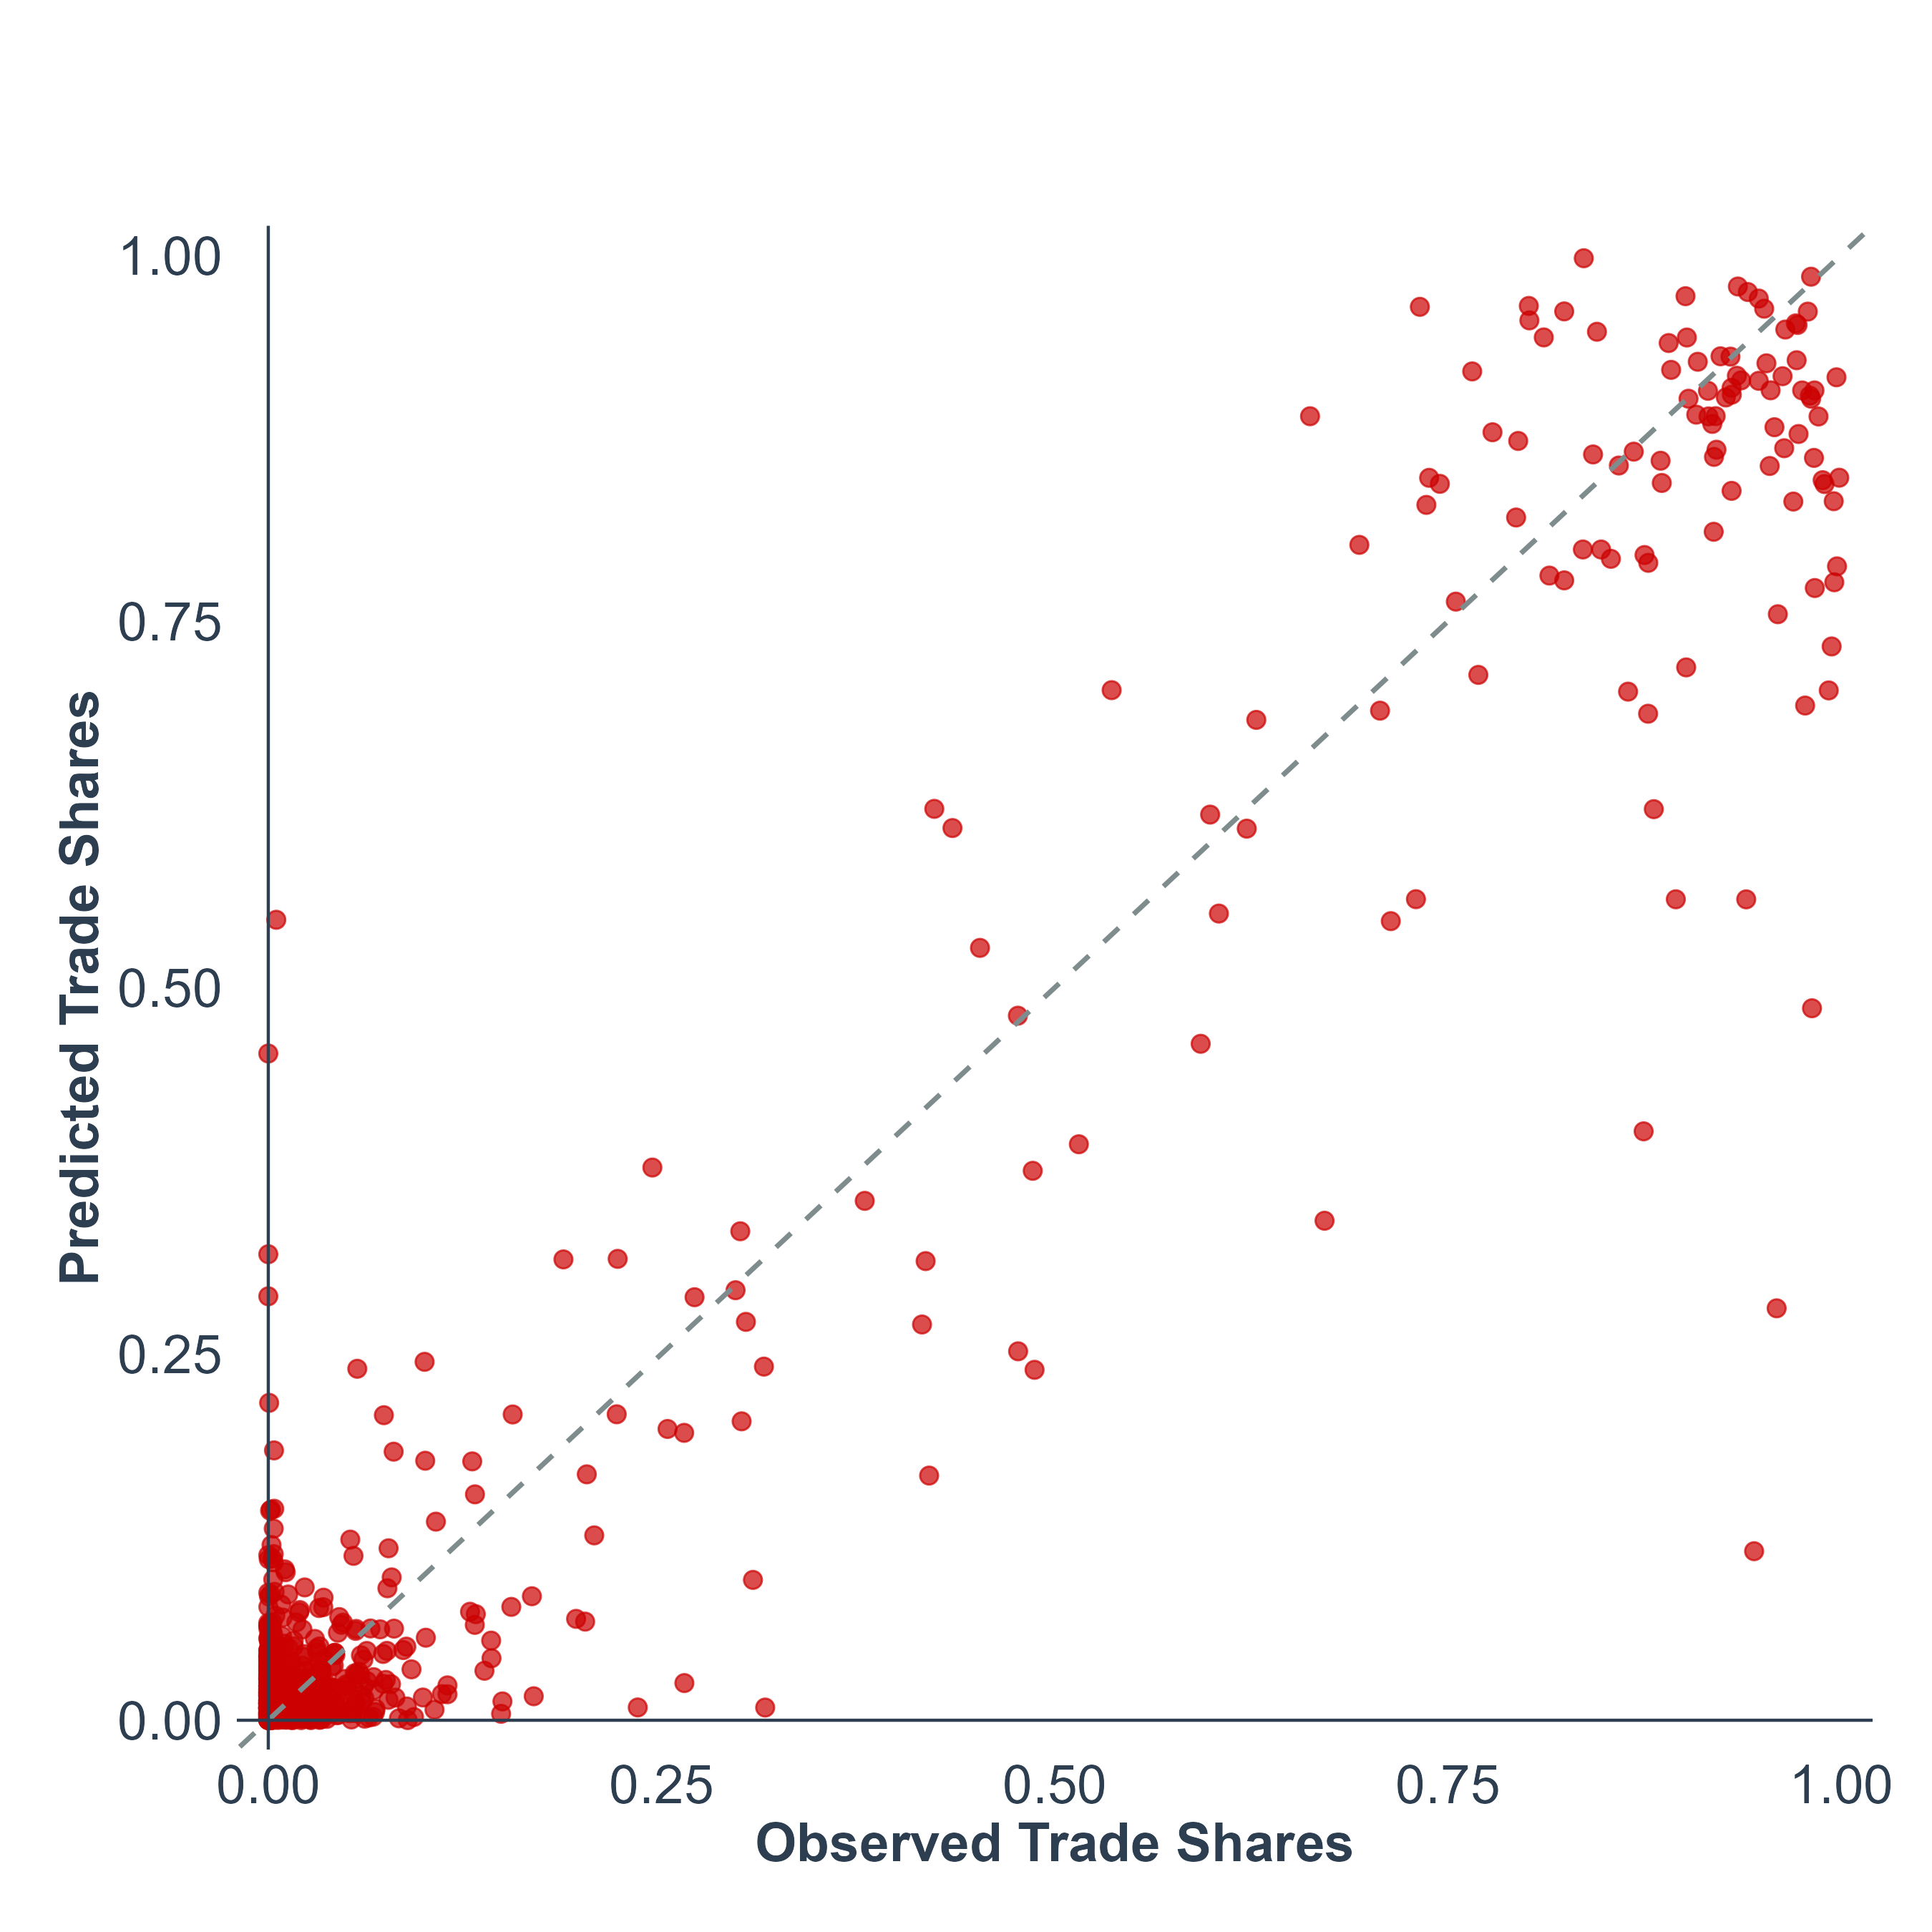
\includegraphics[width=\textwidth]{code/figures/trade_flows_fit_mobile.png}
        \caption{Mobile Sectors}
        \label{fig:trade_flows_fit_mobile}
    \end{subfigure}
    \hfill
    \begin{subfigure}{0.48\textwidth}
        \centering
        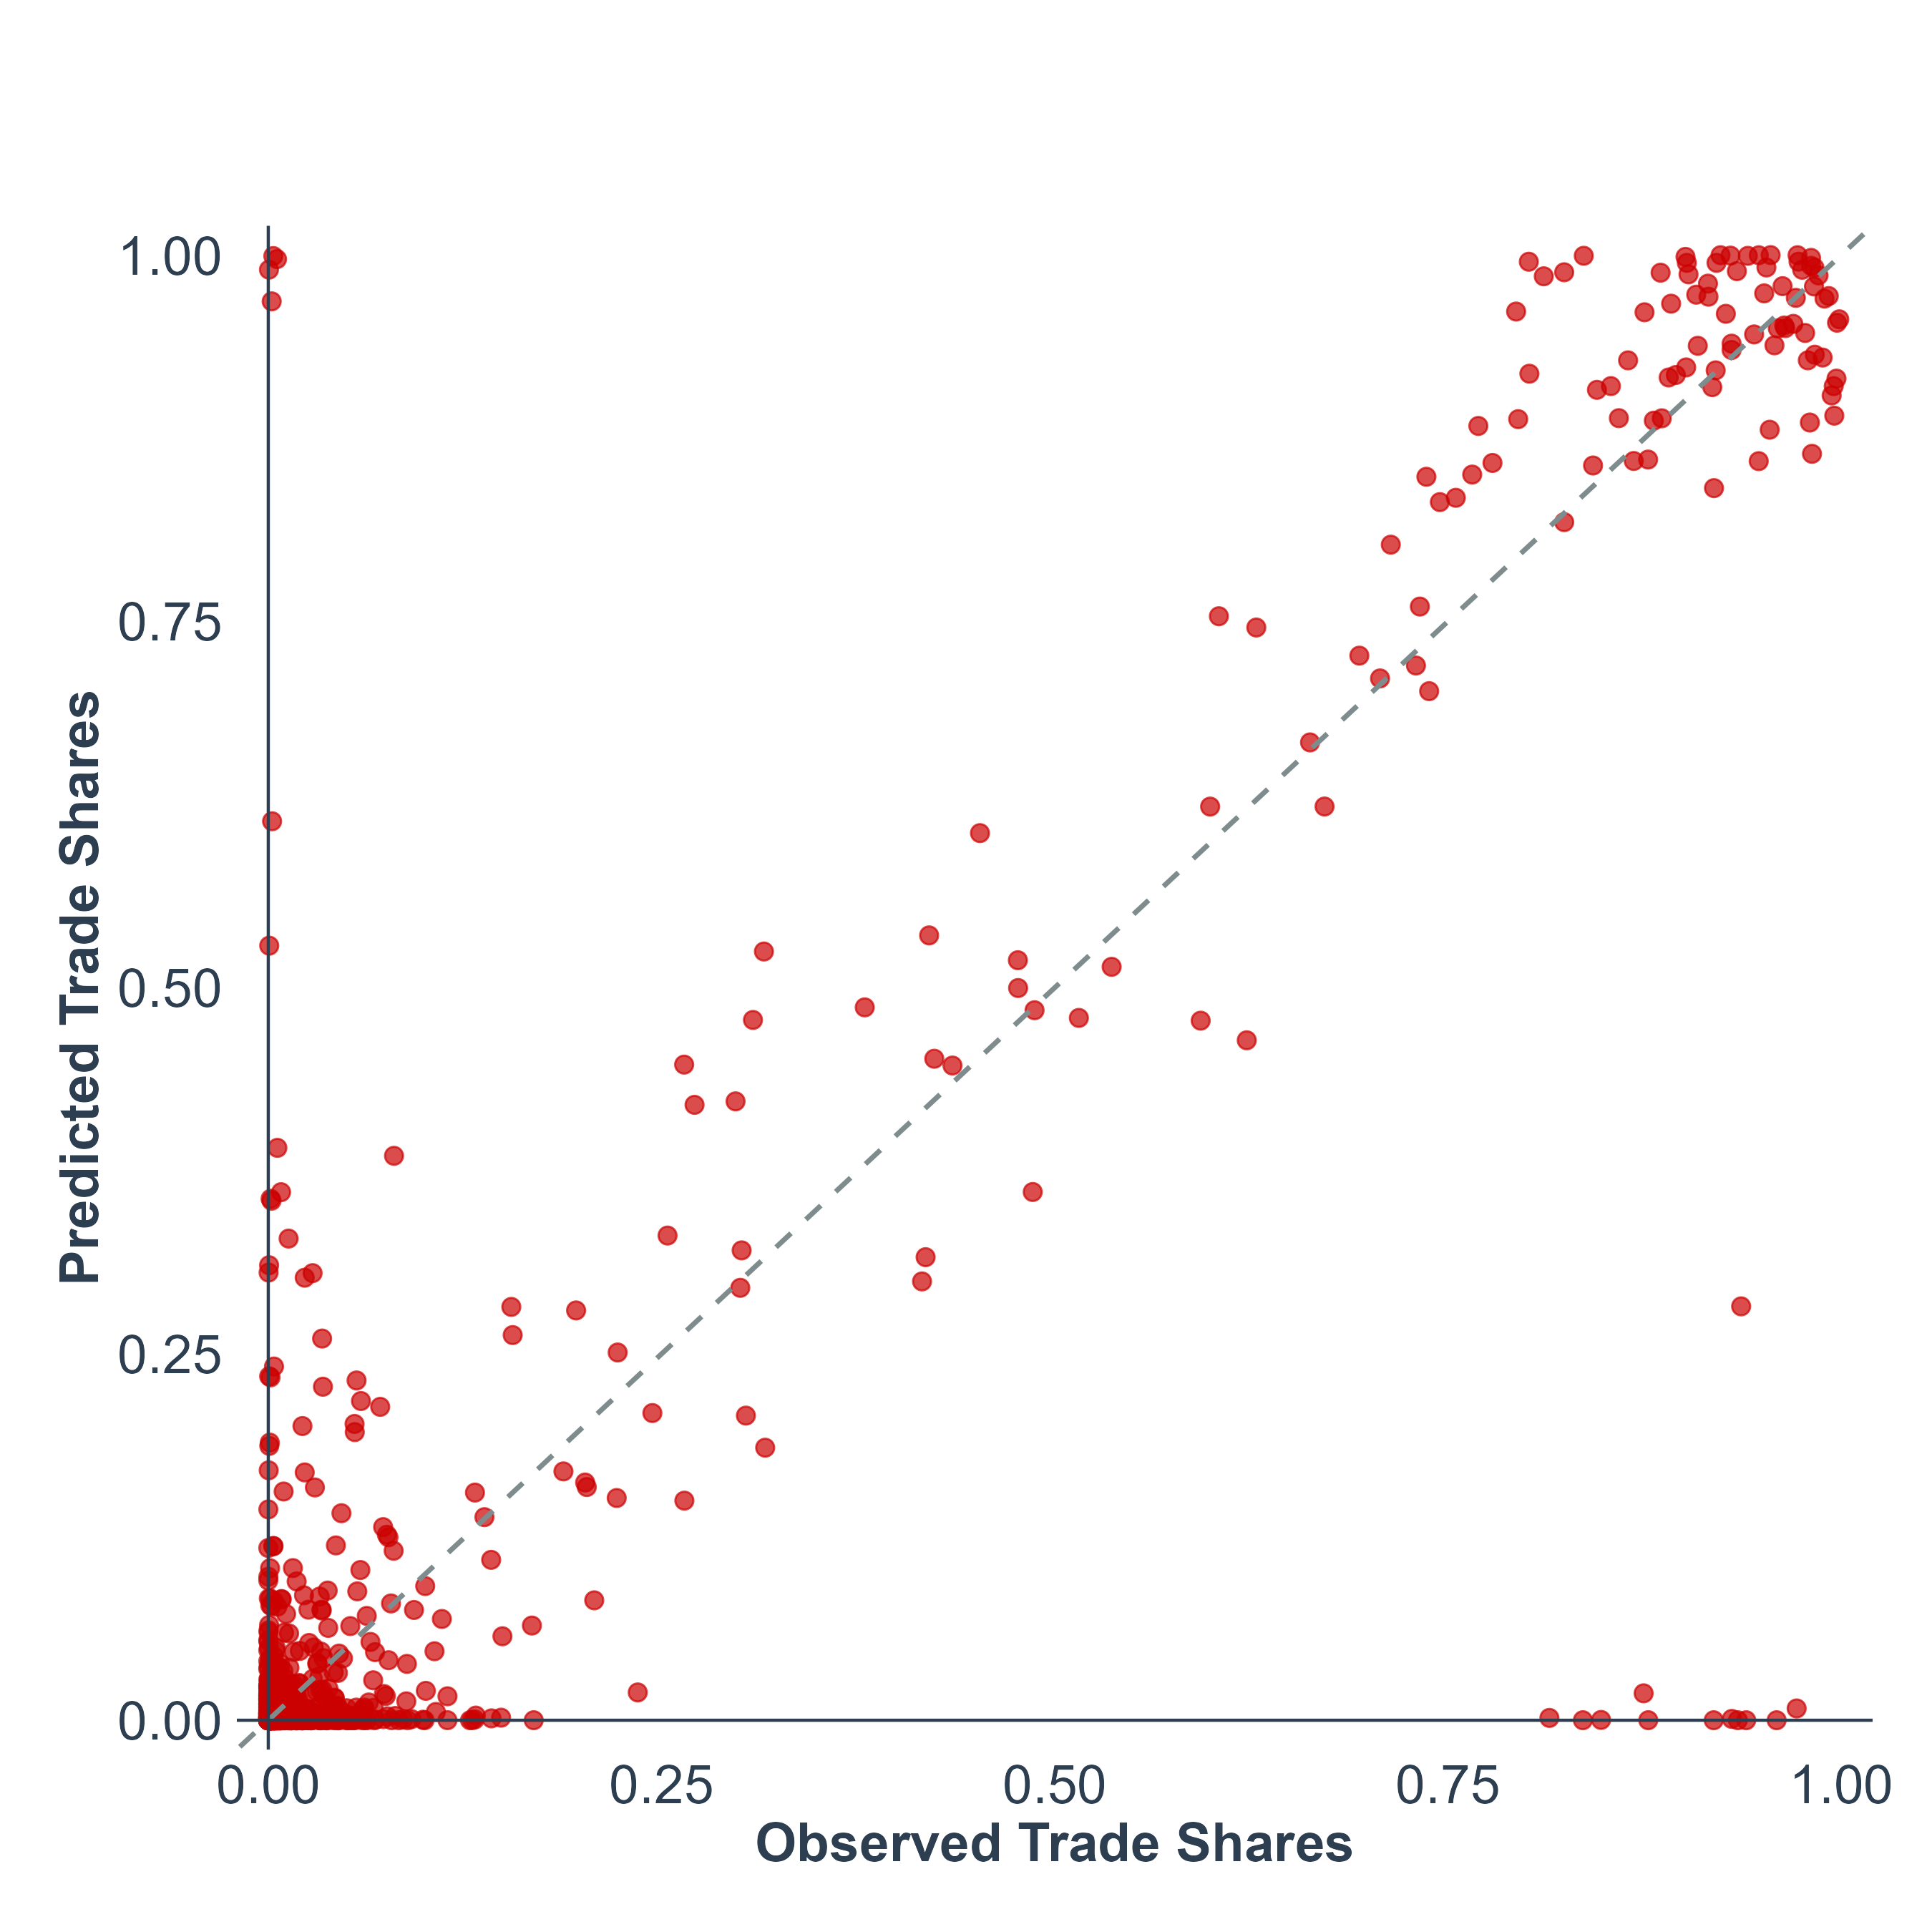
\includegraphics[width=\textwidth]{code/figures/trade_flows_fit_immobile.png}
        \caption{Immobile Sectors}
        \label{fig:trade_flows_fit_immobile}
    \end{subfigure}
    \caption{Model Fit: Predicted vs. Observed Bilateral Trade Shares}
    \label{fig:trade_flows_fit}
\end{figure}

However, when we look at GDP shares, the fit is very poor, as shown in Figure \ref{fig:gdp_fit}. This is likely due to the fact that we are not targeting GDP shares in our calibration, and the model is not flexible enough to match both trade shares and GDP shares simultaneously given the limited number of parameters. This suggests that future work could explore alternative parameterizations or additional data sources to improve the model's ability to replicate observed production patterns while maintaining trade flow accuracy.

\begin{figure}[H]
    \centering
    \begin{subfigure}{0.48\textwidth}
        \centering
        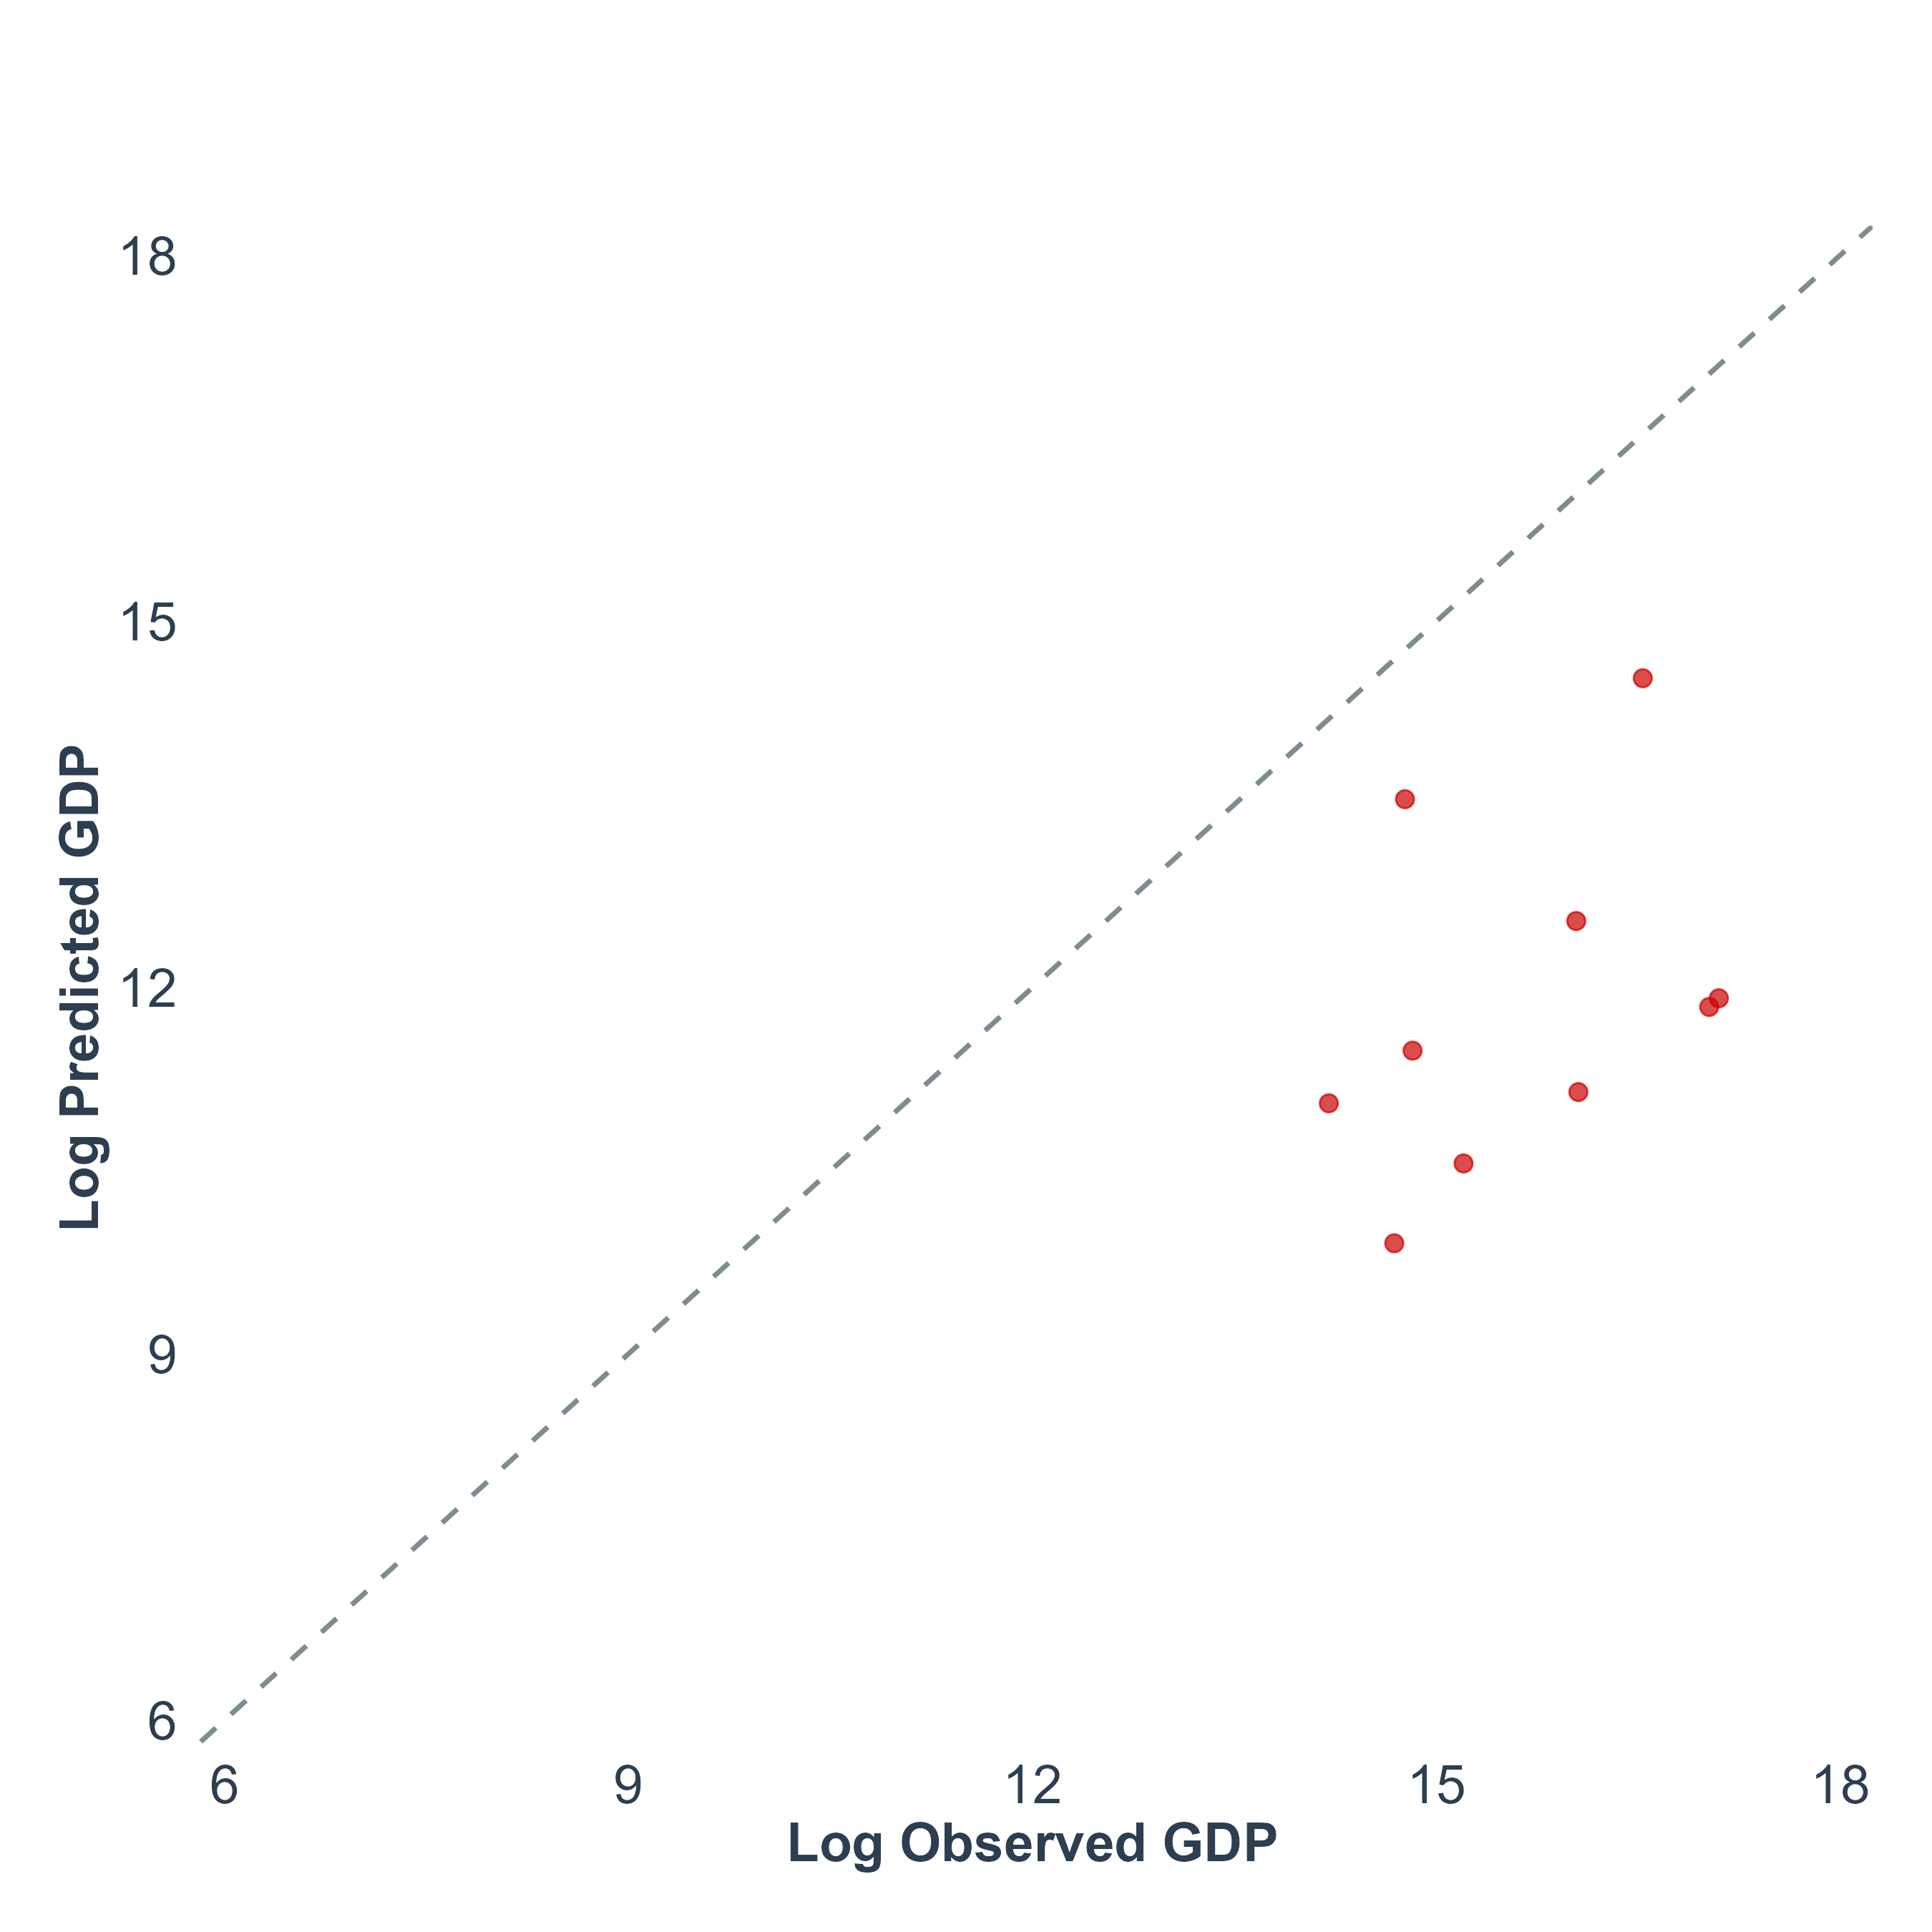
\includegraphics[width=\textwidth]{code/figures/gdp_fit_mobile.png}
        \caption{Mobile Sectors}
        \label{fig:gdp_fit_mobile}
    \end{subfigure}
    \hfill
    \begin{subfigure}{0.48\textwidth}
        \centering
        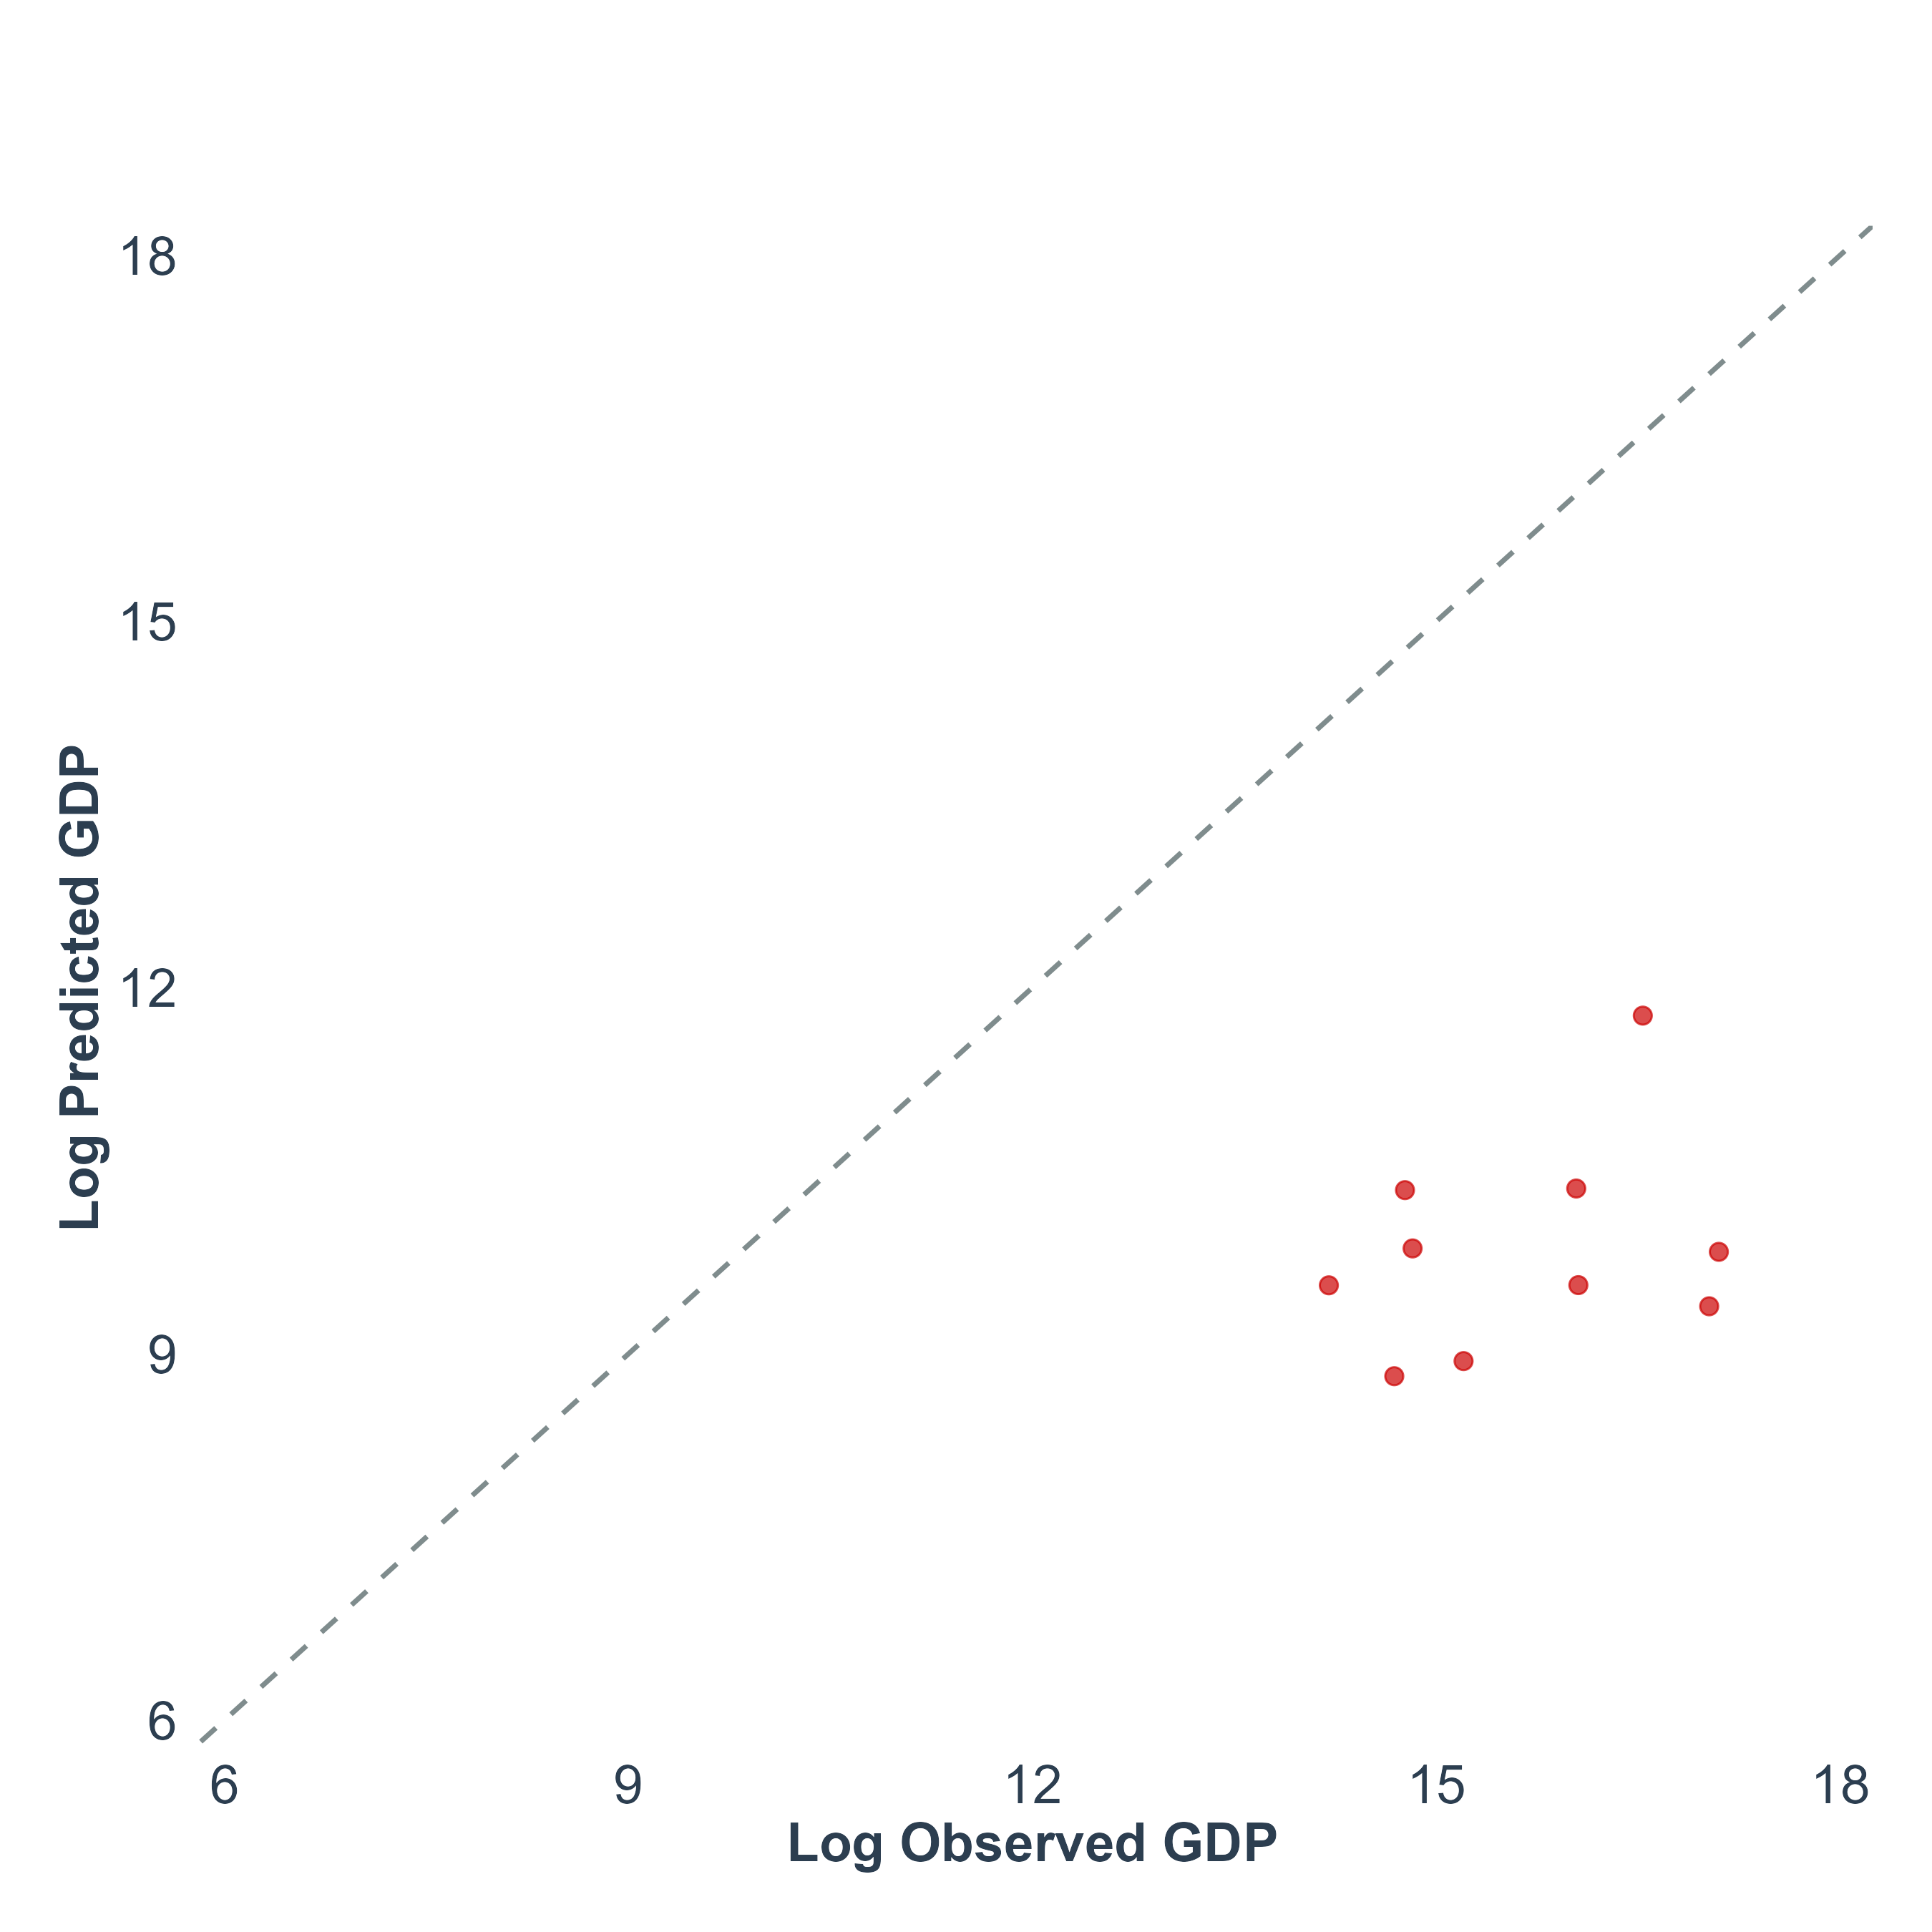
\includegraphics[width=\textwidth]{code/figures/gdp_fit_immobile.png}
        \caption{Immobile Sectors}
        \label{fig:gdp_fit_immobile}
    \end{subfigure}
    \caption{Model Fit: Predicted vs. Observed GDP Shares}
    \label{fig:gdp_fit}
\end{figure}


% The calibrated model satisfies all equilibrium conditions within numerical tolerance. Trade balance is achieved: $\sum_{i,k} \pi_{ink} X_{ik} - \sum_{i,k} \pi_{nik} X_{nk} = 0$ for all countries, and price consistency relationships are verified: the sectoral price indices $p_{nk} = \left[\sum_{i} \left(\frac{c_{ik}(1+\tau_{nik})d_{nik}}{T_{ik}^{1/\theta}}\right)^{-\theta}\right]^{-1/\theta}$ match computed values. \newpage
\section{Counterfactual Analysis}

This section evaluates the economic effects of alternative tariff policies using our calibrated multi-sector model. We analyze three contemporary scenarios based on 2025 US trade data: Last Twelve Months (LTM), Year-to-Date (YTD), and Most Recent Quarter (3M) tariff rates. Each scenario is evaluated under both mobile and immobile labor assumptions to capture short-run versus long-run adjustment mechanisms.

\subsection{Policy Scenarios}

Our counterfactual experiments replace the baseline 2024 tariff structure with contemporary rates derived from HTS-level US import data. The three scenarios capture different temporal perspectives on recent trade policy:
\textbf{LTM Scenario (Last Twelve Months):} Uses contemporary tariff rates based on recent US trade policy implementation. This scenario captures the current protective stance across sectors.

\textbf{YTD Scenario (Year-to-Date):} Employs tariff rates reflecting policy changes implemented during 2025. This scenario provides the baseline for our main counterfactual analysis.

\textbf{3M Scenario (Recent Quarter):} Focuses on the most recent policy adjustments, highlighting short-term trade impacts and immediate policy effects.

These scenarios are compared against the 2024 baseline to quantify the welfare and structural adjustment effects of contemporary trade policy. The temporal variation allows analysis of policy evolution and helps identify which time horizon best captures steady-state effects.

Under the mobile labor assumption, workers can reallocate across sectors within each country in response to tariff changes. This represents the long-run equilibrium where factor markets have fully adjusted to policy changes.

The YTD tariff scenario results (Table \ref{tab:welfare_tariff_rate25_YTD_mobile}) show welfare effects that appear implausibly large in magnitude, similar to the immobile labor case. The EU shows gains of 19.58\%, USA 14.37\%, China 7.50\%, Brazil 5.21\%, and Japan 4.76\%, while Mexico faces losses of -4.91\% and Canada -1.28\%.

While the absolute magnitudes are unrealistic and suggest model specification or computational issues, the relative ordering of countries provides meaningful insights. The results indicate that Canada and Mexico are the countries most vulnerable to contemporary US tariff policies, consistent with their deep integration with US supply chains and NAFTA/USMCA trade relationships. Similarly, the model identifies India, China, and Brazil as potentially significant losers from protectionist policies, reflecting their substantial trade exposure to developed markets.

\begin{landscape}
    \vspace*{\fill}
    % latex table generated in R 4.4.3 by xtable 1.8-4 package
% Tue Oct  7 02:00:25 2025
\begin{table}[htbp]
\centering
\caption{Welfare Effects by Country - 2025 YTD Tariffs: with Labor Mobility} 
\label{tab:welfare_tariff_rate25_YTD_mobile}
\begin{tabular}{lccccc}
  \hline
 & Baseline Tariff (p.p.) & Counterfactual Tariff (p.p.) & Welfare Change (\%) & Income Change (\%) & Tariff Revenue Change (\%) \\ 
  \hline
BRA & \textcolor[RGB]{102,66,153}{2.870} & \textcolor[RGB]{92,59,163}{3.080} & \textcolor[RGB]{56,36,199}{5.210} & \textcolor[RGB]{51,33,204}{5.270} & \textcolor[RGB]{240,155,15}{-5.490} \\ 
  CAN & \textcolor[RGB]{133,86,122}{2.260} & \textcolor[RGB]{138,89,117}{2.110} & \textcolor[RGB]{219,142,36}{-1.280} & \textcolor[RGB]{224,145,31}{-1.300} & \textcolor[RGB]{77,50,178}{4.290} \\ 
  CHN & \textcolor[RGB]{189,122,66}{0.540} & \textcolor[RGB]{194,125,61}{0.490} & \textcolor[RGB]{41,26,214}{7.500} & \textcolor[RGB]{46,30,209}{7.450} & \textcolor[RGB]{5,3,250}{42.660} \\ 
  EU & \textcolor[RGB]{168,109,87}{1.630} & \textcolor[RGB]{148,96,107}{1.800} & \textcolor[RGB]{10,7,245}{19.580} & \textcolor[RGB]{10,7,245}{19.580} & \textcolor[RGB]{0,0,255}{44.660} \\ 
  GBR & \textcolor[RGB]{143,92,112}{1.830} & \textcolor[RGB]{158,102,97}{1.770} & \textcolor[RGB]{112,73,143}{2.730} & \textcolor[RGB]{117,76,138}{2.720} & \textcolor[RGB]{20,13,235}{14.690} \\ 
  IND & \textcolor[RGB]{199,129,56}{0.290} & \textcolor[RGB]{199,129,56}{0.290} & \textcolor[RGB]{122,79,133}{2.650} & \textcolor[RGB]{128,82,128}{2.600} & \textcolor[RGB]{36,23,219}{9.150} \\ 
  JPN & \textcolor[RGB]{107,69,148}{2.810} & \textcolor[RGB]{97,63,158}{2.940} & \textcolor[RGB]{71,46,184}{4.760} & \textcolor[RGB]{66,43,189}{4.770} & \textcolor[RGB]{245,158,10}{-5.860} \\ 
  MEX & \textcolor[RGB]{173,112,82}{1.430} & \textcolor[RGB]{178,115,76}{1.340} & \textcolor[RGB]{230,148,26}{-4.910} & \textcolor[RGB]{235,152,20}{-4.940} & \textcolor[RGB]{184,119,71}{0.730} \\ 
  RoW & \textcolor[RGB]{61,40,194}{4.990} & \textcolor[RGB]{87,56,168}{3.680} & \textcolor[RGB]{163,106,92}{1.760} & \textcolor[RGB]{153,99,102}{1.780} & \textcolor[RGB]{250,162,5}{-6.140} \\ 
  USA & \textcolor[RGB]{255,165,0}{0.000} & \textcolor[RGB]{255,165,0}{0.000} & \textcolor[RGB]{31,20,224}{14.370} & \textcolor[RGB]{25,16,230}{14.410} & \textcolor[RGB]{82,53,173}{3.770} \\ 
   \hline
\end{tabular}
\end{table}

    \vspace*{\fill}
\end{landscape}
The pattern where North American trading partners (Canada, Mexico) show the largest relative welfare losses aligns with expectations that geographically proximate and economically integrated countries face the greatest adjustment costs from trade disruptions. This ordering effect, rather than the specific numerical values, represents the most reliable insight from this counterfactual exercise.

Tariff revenue changes also show implausibly large magnitudes, with EU increasing 44.66\% and China 42.66\%, while Brazil (-5.49\%), Japan (-5.86\%), and Rest of World (-6.14\%) experience decreases. Again, the levels are unrealistic, but the pattern suggests differential impacts across trading partners that merit further investigation with improved model specifications. We don't believe that these are just general equilibrium effects, but rather numerical issues with the immobile labor specification.

The immobile labor specification assumes workers cannot move between sectors, representing short-run adjustment where sectoral employment remains fixed at baseline levels. This scenario captures immediate policy impacts before factor reallocation occurs.

The immobile labor results (Table \ref{tab:welfare_tariff_rate25_YTD_immobile}) exhibit extremely large welfare effects that appear unrealistic. Canada shows welfare gains of 14,773\%, GBR 7,030\%, and Japan 5,839\%, while even the smallest effects (USA: 112.76\%, China: 94.82\%) are implausibly large. These results suggest numerical instability or specification issues in the immobile labor model.

The magnitude of these welfare changes indicates that the immobile labor constraint may be creating artificial rigidities that generate unrealistic general equilibrium responses. When labor cannot reallocate across sectors, the model appears to compensate through extreme price and wage adjustments that violate economic intuition.

Tariff revenue changes under immobile labor are similarly extreme, with most countries showing increases in the thousands of percent. These results suggest fundamental problems with the immobile labor specification, making the mobile labor scenario more credible for policy analysis.

The implausible welfare effects under labor immobility highlight the importance of factor mobility assumptions in quantitative trade models. The excessive gains may reflect computational difficulties in solving the general equilibrium system under binding employment constraints, indicating that the mobile labor specification provides more reliable counterfactual predictions.
\begin{landscape}
    \vspace*{\fill}
    % latex table generated in R 4.4.3 by xtable 1.8-4 package
% Tue Oct  7 02:12:32 2025
\begin{table}[htbp]
\centering
\caption{Welfare Effects by Country - 2025 YTD Tariffs: without Labor Mobility} 
\label{tab:welfare_tariff_rate25_YTD_immobile}
\begin{tabular}{lccccc}
  \hline
 & Baseline Tariff (p.p.) & Counterfactual Tariff (p.p.) & Welfare Change (\%) & Income Change (\%) & Tariff Revenue Change (\%) \\ 
  \hline
BRA & \textcolor[RGB]{199,129,56}{2.840} & \textcolor[RGB]{163,106,92}{8.400} & \textcolor[RGB]{46,30,209}{4359.050} & \textcolor[RGB]{51,33,204}{4268.170} & \textcolor[RGB]{15,10,240}{9960.980} \\ 
  CAN & \textcolor[RGB]{214,139,41}{2.110} & \textcolor[RGB]{189,122,66}{3.530} & \textcolor[RGB]{5,3,250}{14773.460} & \textcolor[RGB]{10,7,245}{14731.570} & \textcolor[RGB]{0,0,255}{24494.880} \\ 
  CHN & \textcolor[RGB]{158,102,97}{8.780} & \textcolor[RGB]{153,99,102}{13.790} & \textcolor[RGB]{133,86,122}{94.820} & \textcolor[RGB]{138,89,117}{94.780} & \textcolor[RGB]{102,66,153}{230.300} \\ 
  EU & \textcolor[RGB]{173,112,82}{5.280} & \textcolor[RGB]{194,125,61}{3.040} & \textcolor[RGB]{143,92,112}{28.300} & \textcolor[RGB]{143,92,112}{28.300} & \textcolor[RGB]{112,73,143}{206.330} \\ 
  GBR & \textcolor[RGB]{230,148,26}{0.540} & \textcolor[RGB]{178,115,76}{4.670} & \textcolor[RGB]{25,16,230}{7030.070} & \textcolor[RGB]{20,13,235}{7042.520} & \textcolor[RGB]{56,36,199}{3122.370} \\ 
  IND & \textcolor[RGB]{240,155,15}{0.030} & \textcolor[RGB]{209,135,46}{2.430} & \textcolor[RGB]{61,40,194}{2669.430} & \textcolor[RGB]{66,43,189}{2595.920} & \textcolor[RGB]{41,26,214}{4433.030} \\ 
  JPN & \textcolor[RGB]{224,145,31}{0.680} & \textcolor[RGB]{168,109,87}{8.000} & \textcolor[RGB]{36,23,219}{5838.970} & \textcolor[RGB]{31,20,224}{5865.050} & \textcolor[RGB]{82,53,173}{1632.200} \\ 
  MEX & \textcolor[RGB]{235,152,20}{0.430} & \textcolor[RGB]{204,132,51}{2.590} & \textcolor[RGB]{87,56,168}{1631.290} & \textcolor[RGB]{77,50,178}{1646.680} & \textcolor[RGB]{92,59,163}{619.100} \\ 
  RoW & \textcolor[RGB]{184,119,71}{4.290} & \textcolor[RGB]{219,142,36}{1.190} & \textcolor[RGB]{107,69,148}{209.960} & \textcolor[RGB]{117,76,138}{205.550} & \textcolor[RGB]{71,46,184}{2374.150} \\ 
  USA & \textcolor[RGB]{255,165,0}{0.000} & \textcolor[RGB]{255,165,0}{0.000} & \textcolor[RGB]{122,79,133}{112.760} & \textcolor[RGB]{128,82,128}{109.150} & \textcolor[RGB]{97,63,158}{418.400} \\ 
   \hline
\end{tabular}
\end{table}

    \vspace*{\fill}
\end{landscape}


\subsection{Policy Implications}

The YTD scenario analysis reveals several key policy insights. The asymmetric welfare distribution suggests that contemporary trade policies generate significant redistributive effects across countries. The main source of welfare gains appears to be trade diversion, where protected domestic industries benefit at the expense of foreign competitors. By imposing tariffs, the US may be redirecting trade flows towards its own producers, thereby improving its terms of trade. However, this comes at the cost of efficiency losses in global supply chains, particularly affecting countries like Canada and Mexico that are closely integrated with the US economy.

The contrast between mobile and immobile labor scenarios highlights the critical importance of labor market flexibility in determining adjustment costs. While the mobile labor results suggest manageable welfare effects ranging from -4.91\% to +19.58\%, the implausible immobile labor results indicate that rigid labor markets could generate severe adjustment problems.

\newpage
\section{Conclusion}

This study applies the \cite{costinot2012TheReviewofEconomicStudies} multi-sector Ricardian trade model to examine U.S. tariff policies using WIOD input-output data and U.S. tariff information. The analysis covers 10 countries and 12 sectors, revealing asymmetric welfare effects under the 2025 YTD tariff scenario. With mobile labor, the model predicts welfare gains of 19.58\% for the European Union and 14.37\% for the United States, while showing losses of 4.91\% for Mexico and 1.28\% for Canada. These results suggest that trade policies redistribute welfare across countries, with larger economies potentially benefiting at the expense of smaller, trade-dependent partners.

The calibration strategy combines input-output data with trade policy information, achieving reasonable fit to bilateral trade patterns ($R^2 = 0.933$). However, the model struggles to match GDP shares simultaneously, indicating trade-offs between trade flow accuracy and production pattern replication. The immobile labor specification produces implausibly large welfare changes, suggesting numerical issues and highlighting the importance of labor mobility assumptions in these models.

The results indicate that the examined tariff policies function more as redistributive mechanisms than efficiency improvements. While the welfare effects are substantial, ranging from losses of nearly 5\% to gains exceeding 19\%, these findings should be interpreted cautiously given the model's limitations. The contrast between mobile and immobile labor results emphasizes the role of labor market assumptions in determining policy impacts. Future work could address computational challenges in solving constrained equilibrium models and estimate more precisely what are the policy shocks driving these welfare changes.

% --- Bibliography ---
\newpage
\bibliography{references}
\bibliographystyle{chicago}

% % --- Appendix ---
\newpage
\section*{Appendix}

This appendix contains the estimated parameters and data tables used in the analysis.

\paragraph{Estimated Parameters}
Tables~\ref{tab:alpha} and~\ref{tab:beta} present the estimated preference parameters and labor share parameters for each country and sector.

\paragraph{Technology Parameters}
Tables~\ref{tab:gamma_BRA} through~\ref{tab:gamma_USA} show the intermediate input coefficients for each country.

\paragraph{Productivity Parameters}
Table~\ref{tab:technology} presents the productivity parameters used in the model calibration.

\paragraph{Tariff Data}
Tables~\ref{tab:tariff_BRA} through~\ref{tab:tariff_USA} contain the tariff rates applied by each country across different sectors.

\paragraph{Trade Cost Decomposition}
Tables~\ref{tab:bilateral_costs}, \ref{tab:exporter_effects}, and \ref{tab:importer_effects} provide the decomposition of iceberg trade costs into bilateral, exporter, and importer components. Tables~\ref{tab:iceberg_Chemical} through~\ref{tab:iceberg_Transport} present the final estimated iceberg trade costs for each sector.

\paragraph{Welfare Effects}
Tables~\ref{tab:welfare_tariff_rate25_3M_mobile} through~\ref{tab:welfare_tariff_rate25_LTM_immobile} summarize the welfare effects of other tariff scenarios under both mobile and immobile labor assumptions.

\begin{landscape}
\vspace*{\fill}
% latex table generated in R 4.4.3 by xtable 1.8-4 package
% Tue Oct  7 01:55:00 2025
\begin{table}[htbp]
\centering
\caption{Expenditure Shares ($\alpha$)} 
\label{tab:alpha}
\begin{tabular}{lcccccccccccc}
  \hline
 & Chemical & Construction & Energy & Food & Manufacture & Metal & Mining & Paper & Retail & Services & Textiles & Transport \\ 
  \hline
BRA & \textcolor[RGB]{94,61,162}{0.082} & \textcolor[RGB]{174,113,81}{0.047} & \textcolor[RGB]{74,48,181}{0.096} & \textcolor[RGB]{32,21,223}{0.117} & \textcolor[RGB]{110,72,144}{0.075} & \textcolor[RGB]{100,65,155}{0.079} & \textcolor[RGB]{178,115,76}{0.046} & \textcolor[RGB]{225,146,30}{0.030} & \textcolor[RGB]{55,36,200}{0.105} & \textcolor[RGB]{11,7,244}{0.245} & \textcolor[RGB]{238,154,17}{0.015} & \textcolor[RGB]{132,85,123}{0.063} \\ 
  CAN & \textcolor[RGB]{151,98,104}{0.055} & \textcolor[RGB]{140,91,115}{0.059} & \textcolor[RGB]{176,114,79}{0.047} & \textcolor[RGB]{142,92,113}{0.059} & \textcolor[RGB]{89,58,166}{0.086} & \textcolor[RGB]{108,70,147}{0.077} & \textcolor[RGB]{104,67,151}{0.078} & \textcolor[RGB]{164,106,91}{0.052} & \textcolor[RGB]{23,15,232}{0.137} & \textcolor[RGB]{8,5,246}{0.289} & \textcolor[RGB]{249,161,6}{0.006} & \textcolor[RGB]{147,95,108}{0.056} \\ 
  CHN & \textcolor[RGB]{40,26,215}{0.112} & \textcolor[RGB]{240,155,15}{0.014} & \textcolor[RGB]{121,78,134}{0.072} & \textcolor[RGB]{53,34,202}{0.107} & \textcolor[RGB]{17,11,238}{0.172} & \textcolor[RGB]{19,12,236}{0.166} & \textcolor[RGB]{134,87,121}{0.061} & \textcolor[RGB]{200,129,55}{0.041} & \textcolor[RGB]{189,122,66}{0.042} & \textcolor[RGB]{28,18,227}{0.123} & \textcolor[RGB]{170,110,85}{0.049} & \textcolor[RGB]{185,120,70}{0.043} \\ 
  EU & \textcolor[RGB]{168,109,87}{0.050} & \textcolor[RGB]{68,44,187}{0.097} & \textcolor[RGB]{130,84,125}{0.063} & \textcolor[RGB]{153,99,102}{0.055} & \textcolor[RGB]{83,54,172}{0.090} & \textcolor[RGB]{102,66,153}{0.078} & \textcolor[RGB]{230,148,26}{0.028} & \textcolor[RGB]{223,144,32}{0.031} & \textcolor[RGB]{45,29,210}{0.109} & \textcolor[RGB]{4,3,251}{0.318} & \textcolor[RGB]{244,158,11}{0.008} & \textcolor[RGB]{117,76,138}{0.073} \\ 
  GBR & \textcolor[RGB]{221,143,34}{0.034} & \textcolor[RGB]{57,37,198}{0.105} & \textcolor[RGB]{183,118,72}{0.043} & \textcolor[RGB]{208,135,47}{0.037} & \textcolor[RGB]{144,94,110}{0.057} & \textcolor[RGB]{206,133,49}{0.038} & \textcolor[RGB]{215,139,40}{0.036} & \textcolor[RGB]{227,147,28}{0.030} & \textcolor[RGB]{62,40,193}{0.100} & \textcolor[RGB]{2,1,253}{0.451} & \textcolor[RGB]{253,164,2}{0.003} & \textcolor[RGB]{128,82,128}{0.066} \\ 
  IND & \textcolor[RGB]{113,73,142}{0.073} & \textcolor[RGB]{195,126,60}{0.041} & \textcolor[RGB]{38,25,217}{0.114} & \textcolor[RGB]{49,32,206}{0.109} & \textcolor[RGB]{51,33,204}{0.108} & \textcolor[RGB]{21,14,234}{0.146} & \textcolor[RGB]{166,107,89}{0.052} & \textcolor[RGB]{234,151,21}{0.021} & \textcolor[RGB]{59,38,196}{0.101} & \textcolor[RGB]{34,22,221}{0.116} & \textcolor[RGB]{232,150,23}{0.025} & \textcolor[RGB]{70,45,185}{0.096} \\ 
  JPN & \textcolor[RGB]{98,63,157}{0.080} & \textcolor[RGB]{187,121,68}{0.042} & \textcolor[RGB]{123,80,132}{0.069} & \textcolor[RGB]{138,89,117}{0.060} & \textcolor[RGB]{42,27,212}{0.109} & \textcolor[RGB]{47,30,208}{0.109} & \textcolor[RGB]{204,132,51}{0.039} & \textcolor[RGB]{210,136,45}{0.037} & \textcolor[RGB]{81,52,174}{0.092} & \textcolor[RGB]{6,4,249}{0.303} & \textcolor[RGB]{246,160,8}{0.007} & \textcolor[RGB]{159,103,96}{0.053} \\ 
  MEX & \textcolor[RGB]{77,50,178}{0.095} & \textcolor[RGB]{193,125,62}{0.042} & \textcolor[RGB]{115,74,140}{0.073} & \textcolor[RGB]{85,55,170}{0.088} & \textcolor[RGB]{30,19,225}{0.122} & \textcolor[RGB]{72,47,183}{0.096} & \textcolor[RGB]{119,77,136}{0.073} & \textcolor[RGB]{217,140,38}{0.034} & \textcolor[RGB]{36,23,219}{0.116} & \textcolor[RGB]{13,8,242}{0.204} & \textcolor[RGB]{236,153,19}{0.016} & \textcolor[RGB]{191,124,64}{0.042} \\ 
  RoW & \textcolor[RGB]{157,102,98}{0.053} & \textcolor[RGB]{181,117,74}{0.044} & \textcolor[RGB]{106,69,149}{0.077} & \textcolor[RGB]{79,51,176}{0.092} & \textcolor[RGB]{66,43,189}{0.098} & \textcolor[RGB]{87,56,168}{0.086} & \textcolor[RGB]{25,16,230}{0.135} & \textcolor[RGB]{212,138,42}{0.036} & \textcolor[RGB]{64,41,191}{0.099} & \textcolor[RGB]{15,10,240}{0.187} & \textcolor[RGB]{242,157,13}{0.012} & \textcolor[RGB]{96,62,159}{0.082} \\ 
  USA & \textcolor[RGB]{155,100,100}{0.053} & \textcolor[RGB]{91,59,164}{0.082} & \textcolor[RGB]{172,111,83}{0.047} & \textcolor[RGB]{162,104,94}{0.052} & \textcolor[RGB]{125,81,130}{0.068} & \textcolor[RGB]{149,96,106}{0.055} & \textcolor[RGB]{198,128,57}{0.041} & \textcolor[RGB]{219,142,36}{0.034} & \textcolor[RGB]{136,88,119}{0.060} & \textcolor[RGB]{0,0,255}{0.464} & \textcolor[RGB]{251,162,4}{0.004} & \textcolor[RGB]{202,131,53}{0.040} \\ 
   \hline
\end{tabular}
\end{table}

\vspace*{\fill}
\end{landscape}
\begin{landscape}
\vspace*{\fill}
% latex table generated in R 4.4.3 by xtable 1.8-4 package
% Tue Oct  7 01:55:00 2025
\begin{table}[htbp]
\centering
\caption{Labor Shares ($\beta$)} 
\label{tab:beta}
\begin{tabular}{lcccccccccccc}
  \hline
 & Chemical & Construction & Energy & Food & Manufacture & Metal & Mining & Paper & Retail & Services & Textiles & Transport \\ 
  \hline
BRA & \textcolor[RGB]{162,104,94}{0.166} & \textcolor[RGB]{106,69,149}{0.220} & \textcolor[RGB]{219,142,36}{0.093} & \textcolor[RGB]{153,99,102}{0.170} & \textcolor[RGB]{121,78,134}{0.206} & \textcolor[RGB]{115,74,140}{0.213} & \textcolor[RGB]{170,110,85}{0.153} & \textcolor[RGB]{81,52,174}{0.258} & \textcolor[RGB]{13,8,242}{0.443} & \textcolor[RGB]{8,5,246}{0.447} & \textcolor[RGB]{74,48,181}{0.276} & \textcolor[RGB]{51,33,204}{0.366} \\ 
  CAN & \textcolor[RGB]{140,91,115}{0.184} & \textcolor[RGB]{144,94,110}{0.174} & \textcolor[RGB]{215,139,40}{0.096} & \textcolor[RGB]{185,120,70}{0.133} & \textcolor[RGB]{128,82,128}{0.203} & \textcolor[RGB]{138,89,117}{0.192} & \textcolor[RGB]{202,131,53}{0.112} & \textcolor[RGB]{77,50,178}{0.267} & \textcolor[RGB]{21,14,234}{0.418} & \textcolor[RGB]{15,10,240}{0.440} & \textcolor[RGB]{38,25,217}{0.391} & \textcolor[RGB]{62,40,193}{0.329} \\ 
  CHN & \textcolor[RGB]{249,161,6}{0.060} & \textcolor[RGB]{200,129,55}{0.113} & \textcolor[RGB]{238,154,17}{0.065} & \textcolor[RGB]{59,38,196}{0.329} & \textcolor[RGB]{236,153,19}{0.067} & \textcolor[RGB]{240,155,15}{0.065} & \textcolor[RGB]{164,106,91}{0.164} & \textcolor[RGB]{227,147,28}{0.081} & \textcolor[RGB]{181,117,74}{0.145} & \textcolor[RGB]{94,61,162}{0.239} & \textcolor[RGB]{221,143,34}{0.085} & \textcolor[RGB]{191,124,64}{0.123} \\ 
  EU & \textcolor[RGB]{159,103,96}{0.166} & \textcolor[RGB]{151,98,104}{0.172} & \textcolor[RGB]{223,144,32}{0.085} & \textcolor[RGB]{85,55,170}{0.250} & \textcolor[RGB]{98,63,157}{0.229} & \textcolor[RGB]{100,65,155}{0.224} & \textcolor[RGB]{119,77,136}{0.211} & \textcolor[RGB]{108,70,147}{0.220} & \textcolor[RGB]{32,21,223}{0.402} & \textcolor[RGB]{4,3,251}{0.451} & \textcolor[RGB]{91,59,164}{0.240} & \textcolor[RGB]{72,47,183}{0.276} \\ 
  GBR & \textcolor[RGB]{70,45,185}{0.296} & \textcolor[RGB]{55,36,200}{0.344} & \textcolor[RGB]{210,136,45}{0.100} & \textcolor[RGB]{68,44,187}{0.310} & \textcolor[RGB]{64,41,191}{0.323} & \textcolor[RGB]{53,34,202}{0.363} & \textcolor[RGB]{204,132,51}{0.106} & \textcolor[RGB]{49,32,206}{0.376} & \textcolor[RGB]{28,18,227}{0.407} & \textcolor[RGB]{47,30,208}{0.377} & \textcolor[RGB]{40,26,215}{0.382} & \textcolor[RGB]{34,22,221}{0.398} \\ 
  IND & \textcolor[RGB]{244,158,11}{0.062} & \textcolor[RGB]{89,58,166}{0.248} & \textcolor[RGB]{251,162,4}{0.059} & \textcolor[RGB]{66,43,189}{0.313} & \textcolor[RGB]{230,148,26}{0.079} & \textcolor[RGB]{232,150,23}{0.069} & \textcolor[RGB]{110,72,144}{0.217} & \textcolor[RGB]{130,84,125}{0.199} & \textcolor[RGB]{0,0,255}{0.555} & \textcolor[RGB]{25,16,230}{0.407} & \textcolor[RGB]{142,92,113}{0.175} & \textcolor[RGB]{166,107,89}{0.155} \\ 
  JPN & \textcolor[RGB]{178,115,76}{0.145} & \textcolor[RGB]{125,81,130}{0.204} & \textcolor[RGB]{242,157,13}{0.063} & \textcolor[RGB]{136,88,119}{0.195} & \textcolor[RGB]{155,100,100}{0.169} & \textcolor[RGB]{176,114,79}{0.148} & \textcolor[RGB]{208,135,47}{0.102} & \textcolor[RGB]{79,51,176}{0.267} & \textcolor[RGB]{23,15,232}{0.411} & \textcolor[RGB]{30,19,225}{0.405} & \textcolor[RGB]{2,1,253}{0.458} & \textcolor[RGB]{11,7,244}{0.443} \\ 
  MEX & \textcolor[RGB]{212,138,42}{0.096} & \textcolor[RGB]{195,126,60}{0.121} & \textcolor[RGB]{246,160,8}{0.061} & \textcolor[RGB]{193,125,62}{0.121} & \textcolor[RGB]{217,140,38}{0.094} & \textcolor[RGB]{225,146,30}{0.084} & \textcolor[RGB]{253,164,2}{0.039} & \textcolor[RGB]{187,121,68}{0.131} & \textcolor[RGB]{132,85,123}{0.195} & \textcolor[RGB]{42,27,212}{0.380} & \textcolor[RGB]{157,102,98}{0.166} & \textcolor[RGB]{117,76,138}{0.211} \\ 
  RoW & \textcolor[RGB]{189,122,66}{0.123} & \textcolor[RGB]{149,96,106}{0.173} & \textcolor[RGB]{234,151,21}{0.068} & \textcolor[RGB]{83,54,172}{0.255} & \textcolor[RGB]{168,109,87}{0.155} & \textcolor[RGB]{198,128,57}{0.119} & \textcolor[RGB]{123,80,132}{0.206} & \textcolor[RGB]{113,73,142}{0.217} & \textcolor[RGB]{45,29,210}{0.378} & \textcolor[RGB]{17,11,238}{0.432} & \textcolor[RGB]{183,118,72}{0.144} & \textcolor[RGB]{96,62,159}{0.230} \\ 
  USA & \textcolor[RGB]{172,111,83}{0.152} & \textcolor[RGB]{147,95,108}{0.173} & \textcolor[RGB]{206,133,49}{0.102} & \textcolor[RGB]{174,113,81}{0.151} & \textcolor[RGB]{87,56,168}{0.250} & \textcolor[RGB]{102,66,153}{0.224} & \textcolor[RGB]{134,87,121}{0.195} & \textcolor[RGB]{104,67,151}{0.221} & \textcolor[RGB]{6,4,249}{0.448} & \textcolor[RGB]{19,12,236}{0.422} & \textcolor[RGB]{57,37,198}{0.338} & \textcolor[RGB]{36,23,219}{0.393} \\ 
   \hline
\end{tabular}
\end{table}

\vspace*{\fill}
\end{landscape}

\begin{landscape}
\vspace*{\fill}
% latex table generated in R 4.4.3 by xtable 1.8-4 package
% Tue Oct  7 01:55:00 2025
\begin{table}[htbp]
\centering
\caption{Intermediate Input Shares ($\gamma$) - BRA} 
\label{tab:gamma_BRA}
\begin{tabular}{lcccccccccccc}
  \hline
 & Chemical & Construction & Energy & Food & Manufacture & Metal & Mining & Paper & Retail & Services & Textiles & Transport \\ 
  \hline
Chemical & \textcolor[RGB]{11,7,244}{0.362} & \textcolor[RGB]{189,123,66}{0.012} & \textcolor[RGB]{42,27,212}{0.126} & \textcolor[RGB]{161,104,94}{0.027} & \textcolor[RGB]{172,111,83}{0.023} & \textcolor[RGB]{147,95,108}{0.033} & \textcolor[RGB]{138,89,117}{0.036} & \textcolor[RGB]{165,107,90}{0.025} & \textcolor[RGB]{37,24,218}{0.138} & \textcolor[RGB]{25,16,230}{0.173} & \textcolor[RGB]{221,143,34}{0.006} & \textcolor[RGB]{131,85,124}{0.039} \\ 
  Construction & \textcolor[RGB]{87,56,168}{0.087} & \textcolor[RGB]{57,37,198}{0.110} & \textcolor[RGB]{149,96,106}{0.033} & \textcolor[RGB]{237,154,18}{0.002} & \textcolor[RGB]{113,73,142}{0.058} & \textcolor[RGB]{12,8,243}{0.362} & \textcolor[RGB]{158,102,97}{0.029} & \textcolor[RGB]{128,82,128}{0.042} & \textcolor[RGB]{46,30,209}{0.123} & \textcolor[RGB]{50,32,205}{0.121} & \textcolor[RGB]{241,156,14}{0.002} & \textcolor[RGB]{154,100,101}{0.031} \\ 
  Energy & \textcolor[RGB]{179,116,76}{0.017} & \textcolor[RGB]{204,132,51}{0.007} & \textcolor[RGB]{18,11,237}{0.311} & \textcolor[RGB]{120,78,135}{0.051} & \textcolor[RGB]{152,99,103}{0.031} & \textcolor[RGB]{202,131,53}{0.008} & \textcolor[RGB]{9,6,246}{0.382} & \textcolor[RGB]{243,157,12}{0.002} & \textcolor[RGB]{110,71,145}{0.060} & \textcolor[RGB]{80,52,175}{0.096} & \textcolor[RGB]{253,164,2}{0.000} & \textcolor[RGB]{140,91,115}{0.034} \\ 
  Food & \textcolor[RGB]{78,50,177}{0.097} & \textcolor[RGB]{211,136,44}{0.007} & \textcolor[RGB]{122,79,133}{0.045} & \textcolor[RGB]{0,0,255}{0.537} & \textcolor[RGB]{197,127,58}{0.010} & \textcolor[RGB]{177,115,78}{0.017} & \textcolor[RGB]{223,144,32}{0.005} & \textcolor[RGB]{198,128,57}{0.009} & \textcolor[RGB]{35,23,220}{0.141} & \textcolor[RGB]{71,46,184}{0.102} & \textcolor[RGB]{234,151,21}{0.002} & \textcolor[RGB]{156,101,99}{0.029} \\ 
  Manufacture & \textcolor[RGB]{90,58,165}{0.084} & \textcolor[RGB]{193,125,62}{0.010} & \textcolor[RGB]{136,88,119}{0.038} & \textcolor[RGB]{239,155,16}{0.002} & \textcolor[RGB]{16,10,239}{0.331} & \textcolor[RGB]{23,15,232}{0.216} & \textcolor[RGB]{236,152,19}{0.002} & \textcolor[RGB]{168,109,87}{0.024} & \textcolor[RGB]{58,38,197}{0.110} & \textcolor[RGB]{34,22,221}{0.146} & \textcolor[RGB]{227,147,28}{0.004} & \textcolor[RGB]{151,97,104}{0.032} \\ 
  Metal & \textcolor[RGB]{97,63,158}{0.078} & \textcolor[RGB]{195,126,60}{0.010} & \textcolor[RGB]{73,47,182}{0.101} & \textcolor[RGB]{232,150,23}{0.003} & \textcolor[RGB]{133,86,122}{0.039} & \textcolor[RGB]{14,9,241}{0.339} & \textcolor[RGB]{53,34,202}{0.120} & \textcolor[RGB]{181,117,74}{0.016} & \textcolor[RGB]{62,40,193}{0.109} & \textcolor[RGB]{32,21,223}{0.150} & \textcolor[RGB]{230,149,25}{0.003} & \textcolor[RGB]{145,94,110}{0.033} \\ 
  Mining & \textcolor[RGB]{143,93,112}{0.034} & \textcolor[RGB]{27,17,228}{0.168} & \textcolor[RGB]{99,64,156}{0.077} & \textcolor[RGB]{244,158,11}{0.002} & \textcolor[RGB]{104,68,151}{0.071} & \textcolor[RGB]{96,62,159}{0.078} & \textcolor[RGB]{81,53,174}{0.095} & \textcolor[RGB]{220,142,35}{0.006} & \textcolor[RGB]{108,70,147}{0.062} & \textcolor[RGB]{21,14,234}{0.303} & \textcolor[RGB]{218,141,37}{0.006} & \textcolor[RGB]{76,49,179}{0.099} \\ 
  Paper & \textcolor[RGB]{51,33,204}{0.121} & \textcolor[RGB]{182,118,73}{0.015} & \textcolor[RGB]{106,69,149}{0.064} & \textcolor[RGB]{39,25,216}{0.136} & \textcolor[RGB]{166,108,89}{0.024} & \textcolor[RGB]{159,103,96}{0.028} & \textcolor[RGB]{228,148,27}{0.004} & \textcolor[RGB]{19,13,236}{0.304} & \textcolor[RGB]{74,48,181}{0.101} & \textcolor[RGB]{30,19,225}{0.158} & \textcolor[RGB]{209,135,46}{0.007} & \textcolor[RGB]{135,87,120}{0.038} \\ 
  Retail & \textcolor[RGB]{174,112,81}{0.021} & \textcolor[RGB]{67,44,188}{0.103} & \textcolor[RGB]{44,29,211}{0.125} & \textcolor[RGB]{225,146,30}{0.004} & \textcolor[RGB]{112,72,143}{0.059} & \textcolor[RGB]{207,134,48}{0.007} & \textcolor[RGB]{250,162,5}{0.001} & \textcolor[RGB]{170,110,85}{0.023} & \textcolor[RGB]{64,41,191}{0.107} & \textcolor[RGB]{5,3,250}{0.420} & \textcolor[RGB]{214,139,41}{0.006} & \textcolor[RGB]{48,31,207}{0.123} \\ 
  Services & \textcolor[RGB]{124,80,131}{0.044} & \textcolor[RGB]{92,60,163}{0.082} & \textcolor[RGB]{83,54,172}{0.088} & \textcolor[RGB]{101,65,154}{0.072} & \textcolor[RGB]{126,81,129}{0.043} & \textcolor[RGB]{200,129,55}{0.008} & \textcolor[RGB]{251,163,4}{0.001} & \textcolor[RGB]{142,92,113}{0.034} & \textcolor[RGB]{89,57,166}{0.084} & \textcolor[RGB]{4,2,251}{0.435} & \textcolor[RGB]{212,138,42}{0.006} & \textcolor[RGB]{69,45,186}{0.102} \\ 
  Textiles & \textcolor[RGB]{85,55,170}{0.088} & \textcolor[RGB]{188,121,67}{0.013} & \textcolor[RGB]{115,74,140}{0.055} & \textcolor[RGB]{103,66,152}{0.072} & \textcolor[RGB]{175,113,80}{0.019} & \textcolor[RGB]{205,133,50}{0.007} & \textcolor[RGB]{248,160,7}{0.001} & \textcolor[RGB]{186,120,69}{0.013} & \textcolor[RGB]{28,18,227}{0.161} & \textcolor[RGB]{60,39,195}{0.109} & \textcolor[RGB]{2,1,253}{0.436} & \textcolor[RGB]{163,105,92}{0.026} \\ 
  Transport & \textcolor[RGB]{129,84,126}{0.040} & \textcolor[RGB]{119,77,136}{0.051} & \textcolor[RGB]{41,26,214}{0.134} & \textcolor[RGB]{184,119,71}{0.015} & \textcolor[RGB]{94,61,161}{0.081} & \textcolor[RGB]{216,140,39}{0.006} & \textcolor[RGB]{246,159,9}{0.001} & \textcolor[RGB]{117,76,138}{0.052} & \textcolor[RGB]{66,42,189}{0.105} & \textcolor[RGB]{7,5,248}{0.385} & \textcolor[RGB]{191,124,64}{0.011} & \textcolor[RGB]{55,36,200}{0.120} \\ 
   \hline
\end{tabular}
\end{table}

\vspace*{\fill}
\newpage
\vspace*{\fill}
% latex table generated in R 4.4.3 by xtable 1.8-4 package
% Tue Oct  7 01:55:00 2025
\begin{table}[htbp]
\centering
\caption{Intermediate Input Shares ($\gamma$) - CAN} 
\label{tab:gamma_CAN}
\begin{tabular}{lcccccccccccc}
  \hline
 & Chemical & Construction & Energy & Food & Manufacture & Metal & Mining & Paper & Retail & Services & Textiles & Transport \\ 
  \hline
Chemical & \textcolor[RGB]{12,8,243}{0.407} & \textcolor[RGB]{168,109,87}{0.020} & \textcolor[RGB]{55,36,200}{0.123} & \textcolor[RGB]{195,126,60}{0.013} & \textcolor[RGB]{188,121,67}{0.014} & \textcolor[RGB]{163,105,92}{0.021} & \textcolor[RGB]{92,60,163}{0.058} & \textcolor[RGB]{166,108,89}{0.020} & \textcolor[RGB]{37,24,218}{0.157} & \textcolor[RGB]{53,34,202}{0.128} & \textcolor[RGB]{221,143,34}{0.007} & \textcolor[RGB]{131,85,124}{0.032} \\ 
  Construction & \textcolor[RGB]{113,73,142}{0.043} & \textcolor[RGB]{58,38,197}{0.117} & \textcolor[RGB]{122,79,133}{0.036} & \textcolor[RGB]{204,132,51}{0.010} & \textcolor[RGB]{83,54,172}{0.071} & \textcolor[RGB]{28,18,227}{0.188} & \textcolor[RGB]{74,48,181}{0.079} & \textcolor[RGB]{62,40,193}{0.106} & \textcolor[RGB]{64,41,191}{0.104} & \textcolor[RGB]{21,14,234}{0.221} & \textcolor[RGB]{223,144,32}{0.006} & \textcolor[RGB]{174,112,81}{0.019} \\ 
  Energy & \textcolor[RGB]{152,99,103}{0.023} & \textcolor[RGB]{128,82,128}{0.033} & \textcolor[RGB]{110,71,145}{0.046} & \textcolor[RGB]{241,156,14}{0.003} & \textcolor[RGB]{202,131,53}{0.011} & \textcolor[RGB]{209,135,46}{0.009} & \textcolor[RGB]{0,0,255}{0.670} & \textcolor[RGB]{228,148,27}{0.005} & \textcolor[RGB]{71,46,184}{0.087} & \textcolor[RGB]{90,58,165}{0.060} & \textcolor[RGB]{253,164,2}{0.000} & \textcolor[RGB]{96,62,159}{0.054} \\ 
  Food & \textcolor[RGB]{94,61,161}{0.058} & \textcolor[RGB]{142,92,113}{0.028} & \textcolor[RGB]{115,74,140}{0.040} & \textcolor[RGB]{11,7,244}{0.430} & \textcolor[RGB]{189,123,66}{0.014} & \textcolor[RGB]{181,117,74}{0.017} & \textcolor[RGB]{191,124,64}{0.014} & \textcolor[RGB]{136,88,119}{0.030} & \textcolor[RGB]{30,19,225}{0.182} & \textcolor[RGB]{50,32,205}{0.136} & \textcolor[RGB]{244,158,11}{0.003} & \textcolor[RGB]{104,68,151}{0.048} \\ 
  Manufacture & \textcolor[RGB]{112,72,143}{0.045} & \textcolor[RGB]{172,111,83}{0.019} & \textcolor[RGB]{200,129,55}{0.011} & \textcolor[RGB]{237,154,18}{0.004} & \textcolor[RGB]{9,6,246}{0.443} & \textcolor[RGB]{39,25,216}{0.156} & \textcolor[RGB]{211,136,44}{0.009} & \textcolor[RGB]{149,96,106}{0.026} & \textcolor[RGB]{44,29,211}{0.143} & \textcolor[RGB]{60,39,195}{0.115} & \textcolor[RGB]{220,142,35}{0.007} & \textcolor[RGB]{165,107,90}{0.021} \\ 
  Metal & \textcolor[RGB]{154,100,101}{0.023} & \textcolor[RGB]{182,118,73}{0.017} & \textcolor[RGB]{108,70,147}{0.046} & \textcolor[RGB]{243,157,12}{0.003} & \textcolor[RGB]{175,113,80}{0.018} & \textcolor[RGB]{5,3,250}{0.451} & \textcolor[RGB]{32,21,223}{0.179} & \textcolor[RGB]{207,134,48}{0.010} & \textcolor[RGB]{42,27,212}{0.151} & \textcolor[RGB]{78,50,177}{0.075} & \textcolor[RGB]{251,163,4}{0.001} & \textcolor[RGB]{145,94,110}{0.027} \\ 
  Mining & \textcolor[RGB]{170,110,85}{0.020} & \textcolor[RGB]{85,55,170}{0.071} & \textcolor[RGB]{80,52,175}{0.074} & \textcolor[RGB]{225,146,30}{0.006} & \textcolor[RGB]{101,65,154}{0.050} & \textcolor[RGB]{138,89,117}{0.029} & \textcolor[RGB]{18,11,237}{0.253} & \textcolor[RGB]{205,133,50}{0.010} & \textcolor[RGB]{23,15,232}{0.214} & \textcolor[RGB]{19,13,236}{0.238} & \textcolor[RGB]{248,160,7}{0.001} & \textcolor[RGB]{129,84,126}{0.033} \\ 
  Paper & \textcolor[RGB]{99,64,156}{0.051} & \textcolor[RGB]{151,97,104}{0.024} & \textcolor[RGB]{97,63,158}{0.053} & \textcolor[RGB]{27,17,228}{0.191} & \textcolor[RGB]{161,104,94}{0.021} & \textcolor[RGB]{214,139,41}{0.008} & \textcolor[RGB]{179,116,76}{0.017} & \textcolor[RGB]{16,10,239}{0.296} & \textcolor[RGB]{35,23,220}{0.166} & \textcolor[RGB]{41,26,214}{0.153} & \textcolor[RGB]{246,159,9}{0.002} & \textcolor[RGB]{177,115,78}{0.017} \\ 
  Retail & \textcolor[RGB]{87,56,168}{0.066} & \textcolor[RGB]{73,47,182}{0.080} & \textcolor[RGB]{106,69,149}{0.047} & \textcolor[RGB]{186,120,69}{0.016} & \textcolor[RGB]{69,45,186}{0.087} & \textcolor[RGB]{124,80,131}{0.036} & \textcolor[RGB]{193,125,62}{0.013} & \textcolor[RGB]{81,53,174}{0.073} & \textcolor[RGB]{67,44,188}{0.093} & \textcolor[RGB]{7,5,248}{0.450} & \textcolor[RGB]{218,141,37}{0.007} & \textcolor[RGB]{133,86,122}{0.032} \\ 
  Services & \textcolor[RGB]{135,87,120}{0.031} & \textcolor[RGB]{76,49,179}{0.076} & \textcolor[RGB]{117,76,138}{0.039} & \textcolor[RGB]{120,78,135}{0.036} & \textcolor[RGB]{126,81,129}{0.035} & \textcolor[RGB]{230,149,25}{0.005} & \textcolor[RGB]{198,128,57}{0.012} & \textcolor[RGB]{119,77,136}{0.038} & \textcolor[RGB]{48,31,207}{0.140} & \textcolor[RGB]{2,1,253}{0.523} & \textcolor[RGB]{239,155,16}{0.003} & \textcolor[RGB]{89,57,166}{0.063} \\ 
  Textiles & \textcolor[RGB]{66,42,189}{0.095} & \textcolor[RGB]{159,103,96}{0.023} & \textcolor[RGB]{143,93,112}{0.028} & \textcolor[RGB]{216,140,39}{0.008} & \textcolor[RGB]{184,119,71}{0.016} & \textcolor[RGB]{232,150,23}{0.004} & \textcolor[RGB]{212,138,42}{0.009} & \textcolor[RGB]{158,102,97}{0.023} & \textcolor[RGB]{34,22,221}{0.178} & \textcolor[RGB]{57,37,198}{0.121} & \textcolor[RGB]{4,2,251}{0.472} & \textcolor[RGB]{156,101,99}{0.023} \\ 
  Transport & \textcolor[RGB]{197,127,58}{0.013} & \textcolor[RGB]{103,66,152}{0.049} & \textcolor[RGB]{46,30,209}{0.140} & \textcolor[RGB]{236,152,19}{0.004} & \textcolor[RGB]{140,91,115}{0.028} & \textcolor[RGB]{234,151,21}{0.004} & \textcolor[RGB]{147,95,108}{0.027} & \textcolor[RGB]{227,147,28}{0.006} & \textcolor[RGB]{51,33,204}{0.129} & \textcolor[RGB]{25,16,230}{0.202} & \textcolor[RGB]{250,162,5}{0.001} & \textcolor[RGB]{14,9,241}{0.398} \\ 
   \hline
\end{tabular}
\end{table}

\vspace*{\fill}
\newpage
\vspace*{\fill}
% latex table generated in R 4.4.3 by xtable 1.8-4 package
% Tue Oct  7 01:55:00 2025
\begin{table}[htbp]
\centering
\caption{Intermediate Input Shares ($\gamma$) - CHN} 
\label{tab:gamma_CHN}
\begin{tabular}{lcccccccccccc}
  \hline
 & Chemical & Construction & Energy & Food & Manufacture & Metal & Mining & Paper & Retail & Services & Textiles & Transport \\ 
  \hline
Chemical & \textcolor[RGB]{4,2,251}{0.508} & \textcolor[RGB]{243,157,12}{0.004} & \textcolor[RGB]{50,32,205}{0.113} & \textcolor[RGB]{89,57,166}{0.061} & \textcolor[RGB]{128,82,128}{0.036} & \textcolor[RGB]{138,89,117}{0.032} & \textcolor[RGB]{76,49,179}{0.074} & \textcolor[RGB]{166,108,89}{0.021} & \textcolor[RGB]{133,86,122}{0.033} & \textcolor[RGB]{81,53,174}{0.071} & \textcolor[RGB]{177,115,78}{0.018} & \textcolor[RGB]{142,92,113}{0.030} \\ 
  Construction & \textcolor[RGB]{92,60,163}{0.057} & \textcolor[RGB]{161,104,94}{0.021} & \textcolor[RGB]{120,78,135}{0.037} & \textcolor[RGB]{200,129,55}{0.013} & \textcolor[RGB]{51,33,204}{0.111} & \textcolor[RGB]{11,7,244}{0.451} & \textcolor[RGB]{170,110,85}{0.020} & \textcolor[RGB]{117,76,138}{0.038} & \textcolor[RGB]{101,65,154}{0.048} & \textcolor[RGB]{53,34,202}{0.106} & \textcolor[RGB]{214,139,41}{0.009} & \textcolor[RGB]{64,41,191}{0.087} \\ 
  Energy & \textcolor[RGB]{181,117,74}{0.018} & \textcolor[RGB]{251,163,4}{0.001} & \textcolor[RGB]{18,11,237}{0.313} & \textcolor[RGB]{223,144,32}{0.007} & \textcolor[RGB]{62,40,193}{0.091} & \textcolor[RGB]{202,131,53}{0.013} & \textcolor[RGB]{14,9,241}{0.403} & \textcolor[RGB]{237,154,18}{0.004} & \textcolor[RGB]{151,97,104}{0.026} & \textcolor[RGB]{60,39,195}{0.091} & \textcolor[RGB]{227,147,28}{0.006} & \textcolor[RGB]{149,96,106}{0.026} \\ 
  Food & \textcolor[RGB]{66,42,189}{0.081} & \textcolor[RGB]{250,162,5}{0.002} & \textcolor[RGB]{165,107,90}{0.021} & \textcolor[RGB]{0,0,255}{0.701} & \textcolor[RGB]{195,126,60}{0.015} & \textcolor[RGB]{209,135,46}{0.012} & \textcolor[RGB]{244,158,11}{0.004} & \textcolor[RGB]{188,121,67}{0.017} & \textcolor[RGB]{108,70,147}{0.045} & \textcolor[RGB]{83,54,172}{0.071} & \textcolor[RGB]{246,159,9}{0.003} & \textcolor[RGB]{145,94,110}{0.029} \\ 
  Manufacture & \textcolor[RGB]{67,44,188}{0.081} & \textcolor[RGB]{239,155,16}{0.004} & \textcolor[RGB]{156,101,99}{0.022} & \textcolor[RGB]{218,141,37}{0.008} & \textcolor[RGB]{5,3,250}{0.495} & \textcolor[RGB]{23,15,232}{0.209} & \textcolor[RGB]{228,148,27}{0.006} & \textcolor[RGB]{175,113,80}{0.019} & \textcolor[RGB]{96,62,159}{0.050} & \textcolor[RGB]{78,50,177}{0.073} & \textcolor[RGB]{207,134,48}{0.012} & \textcolor[RGB]{159,103,96}{0.021} \\ 
  Metal & \textcolor[RGB]{103,66,152}{0.048} & \textcolor[RGB]{248,160,7}{0.003} & \textcolor[RGB]{58,38,197}{0.097} & \textcolor[RGB]{225,146,30}{0.007} & \textcolor[RGB]{80,52,175}{0.072} & \textcolor[RGB]{12,8,243}{0.431} & \textcolor[RGB]{30,19,225}{0.175} & \textcolor[RGB]{163,105,92}{0.021} & \textcolor[RGB]{119,77,136}{0.038} & \textcolor[RGB]{85,55,170}{0.069} & \textcolor[RGB]{221,143,34}{0.007} & \textcolor[RGB]{135,87,120}{0.033} \\ 
  Mining & \textcolor[RGB]{69,45,186}{0.080} & \textcolor[RGB]{236,152,19}{0.004} & \textcolor[RGB]{25,16,230}{0.185} & \textcolor[RGB]{211,136,44}{0.011} & \textcolor[RGB]{28,18,227}{0.177} & \textcolor[RGB]{48,31,207}{0.118} & \textcolor[RGB]{37,24,218}{0.145} & \textcolor[RGB]{191,124,64}{0.016} & \textcolor[RGB]{129,84,126}{0.034} & \textcolor[RGB]{39,25,216}{0.141} & \textcolor[RGB]{204,132,51}{0.013} & \textcolor[RGB]{74,48,181}{0.076} \\ 
  Paper & \textcolor[RGB]{42,27,212}{0.128} & \textcolor[RGB]{230,149,25}{0.006} & \textcolor[RGB]{124,80,131}{0.036} & \textcolor[RGB]{44,29,211}{0.125} & \textcolor[RGB]{110,71,145}{0.043} & \textcolor[RGB]{158,102,97}{0.022} & \textcolor[RGB]{212,138,42}{0.010} & \textcolor[RGB]{7,5,248}{0.486} & \textcolor[RGB]{113,73,142}{0.040} & \textcolor[RGB]{90,58,165}{0.059} & \textcolor[RGB]{189,123,66}{0.016} & \textcolor[RGB]{143,93,112}{0.030} \\ 
  Retail & \textcolor[RGB]{147,95,108}{0.027} & \textcolor[RGB]{73,47,182}{0.079} & \textcolor[RGB]{122,79,133}{0.037} & \textcolor[RGB]{174,112,81}{0.019} & \textcolor[RGB]{71,46,184}{0.079} & \textcolor[RGB]{241,156,14}{0.004} & \textcolor[RGB]{253,164,2}{0.001} & \textcolor[RGB]{126,81,129}{0.036} & \textcolor[RGB]{154,100,101}{0.023} & \textcolor[RGB]{9,6,246}{0.480} & \textcolor[RGB]{131,85,124}{0.034} & \textcolor[RGB]{27,17,228}{0.183} \\ 
  Services & \textcolor[RGB]{55,36,200}{0.101} & \textcolor[RGB]{97,63,158}{0.049} & \textcolor[RGB]{106,69,149}{0.046} & \textcolor[RGB]{46,30,209}{0.124} & \textcolor[RGB]{35,23,220}{0.149} & \textcolor[RGB]{179,116,76}{0.018} & \textcolor[RGB]{232,150,23}{0.005} & \textcolor[RGB]{87,56,168}{0.066} & \textcolor[RGB]{94,61,161}{0.053} & \textcolor[RGB]{16,10,239}{0.320} & \textcolor[RGB]{140,91,115}{0.030} & \textcolor[RGB]{115,74,140}{0.039} \\ 
  Textiles & \textcolor[RGB]{57,37,198}{0.097} & \textcolor[RGB]{220,142,35}{0.007} & \textcolor[RGB]{168,109,87}{0.020} & \textcolor[RGB]{32,21,223}{0.159} & \textcolor[RGB]{182,118,73}{0.018} & \textcolor[RGB]{216,140,39}{0.008} & \textcolor[RGB]{234,151,21}{0.005} & \textcolor[RGB]{198,128,57}{0.013} & \textcolor[RGB]{152,99,103}{0.025} & \textcolor[RGB]{99,64,156}{0.048} & \textcolor[RGB]{2,1,253}{0.581} & \textcolor[RGB]{186,120,69}{0.018} \\ 
  Transport & \textcolor[RGB]{104,68,151}{0.048} & \textcolor[RGB]{197,127,58}{0.014} & \textcolor[RGB]{21,14,234}{0.244} & \textcolor[RGB]{112,72,143}{0.042} & \textcolor[RGB]{34,22,221}{0.157} & \textcolor[RGB]{172,111,83}{0.020} & \textcolor[RGB]{193,125,62}{0.015} & \textcolor[RGB]{205,133,50}{0.012} & \textcolor[RGB]{136,88,119}{0.033} & \textcolor[RGB]{19,13,236}{0.262} & \textcolor[RGB]{184,119,71}{0.018} & \textcolor[RGB]{41,26,214}{0.135} \\ 
   \hline
\end{tabular}
\end{table}

\vspace*{\fill}
\newpage
\vspace*{\fill}
% latex table generated in R 4.4.3 by xtable 1.8-4 package
% Tue Oct  7 01:55:00 2025
\begin{table}[htbp]
\centering
\caption{Intermediate Input Shares ($\gamma$) - EU} 
\label{tab:gamma_EU}
\begin{tabular}{lcccccccccccc}
  \hline
 & Chemical & Construction & Energy & Food & Manufacture & Metal & Mining & Paper & Retail & Services & Textiles & Transport \\ 
  \hline
Chemical & \textcolor[RGB]{12,8,243}{0.327} & \textcolor[RGB]{181,117,74}{0.021} & \textcolor[RGB]{73,47,182}{0.089} & \textcolor[RGB]{188,121,67}{0.019} & \textcolor[RGB]{138,89,117}{0.035} & \textcolor[RGB]{133,86,122}{0.037} & \textcolor[RGB]{195,126,60}{0.015} & \textcolor[RGB]{182,118,73}{0.021} & \textcolor[RGB]{35,23,220}{0.161} & \textcolor[RGB]{25,16,230}{0.220} & \textcolor[RGB]{214,139,41}{0.006} & \textcolor[RGB]{113,73,142}{0.049} \\ 
  Construction & \textcolor[RGB]{140,91,115}{0.032} & \textcolor[RGB]{11,7,244}{0.356} & \textcolor[RGB]{151,97,104}{0.030} & \textcolor[RGB]{220,142,35}{0.005} & \textcolor[RGB]{94,61,161}{0.057} & \textcolor[RGB]{42,27,212}{0.147} & \textcolor[RGB]{209,135,46}{0.010} & \textcolor[RGB]{156,101,99}{0.029} & \textcolor[RGB]{78,50,177}{0.084} & \textcolor[RGB]{23,15,232}{0.227} & \textcolor[RGB]{243,157,12}{0.002} & \textcolor[RGB]{179,116,76}{0.022} \\ 
  Energy & \textcolor[RGB]{163,105,92}{0.025} & \textcolor[RGB]{131,85,124}{0.038} & \textcolor[RGB]{19,13,236}{0.271} & \textcolor[RGB]{228,148,27}{0.003} & \textcolor[RGB]{142,92,113}{0.032} & \textcolor[RGB]{191,124,64}{0.017} & \textcolor[RGB]{16,10,239}{0.322} & \textcolor[RGB]{221,143,34}{0.005} & \textcolor[RGB]{71,46,184}{0.094} & \textcolor[RGB]{55,36,200}{0.130} & \textcolor[RGB]{253,164,2}{0.001} & \textcolor[RGB]{90,58,165}{0.062} \\ 
  Food & \textcolor[RGB]{120,78,135}{0.046} & \textcolor[RGB]{186,120,69}{0.020} & \textcolor[RGB]{104,68,151}{0.052} & \textcolor[RGB]{2,1,253}{0.434} & \textcolor[RGB]{177,115,78}{0.022} & \textcolor[RGB]{166,108,89}{0.024} & \textcolor[RGB]{232,150,23}{0.003} & \textcolor[RGB]{184,119,71}{0.021} & \textcolor[RGB]{32,21,223}{0.177} & \textcolor[RGB]{41,26,214}{0.150} & \textcolor[RGB]{239,155,16}{0.002} & \textcolor[RGB]{117,76,138}{0.048} \\ 
  Manufacture & \textcolor[RGB]{97,63,158}{0.055} & \textcolor[RGB]{168,109,87}{0.023} & \textcolor[RGB]{175,113,80}{0.023} & \textcolor[RGB]{230,149,25}{0.003} & \textcolor[RGB]{9,6,246}{0.364} & \textcolor[RGB]{34,22,221}{0.166} & \textcolor[RGB]{236,152,19}{0.002} & \textcolor[RGB]{172,111,83}{0.023} & \textcolor[RGB]{50,32,205}{0.138} & \textcolor[RGB]{37,24,218}{0.159} & \textcolor[RGB]{212,138,42}{0.006} & \textcolor[RGB]{135,87,120}{0.037} \\ 
  Metal & \textcolor[RGB]{129,84,126}{0.039} & \textcolor[RGB]{159,103,96}{0.026} & \textcolor[RGB]{87,56,168}{0.063} & \textcolor[RGB]{234,151,21}{0.003} & \textcolor[RGB]{81,53,174}{0.074} & \textcolor[RGB]{5,3,250}{0.418} & \textcolor[RGB]{106,69,149}{0.052} & \textcolor[RGB]{202,131,53}{0.013} & \textcolor[RGB]{57,37,198}{0.128} & \textcolor[RGB]{53,34,202}{0.130} & \textcolor[RGB]{241,156,14}{0.002} & \textcolor[RGB]{108,70,147}{0.051} \\ 
  Mining & \textcolor[RGB]{128,82,128}{0.042} & \textcolor[RGB]{112,72,143}{0.049} & \textcolor[RGB]{39,25,216}{0.158} & \textcolor[RGB]{216,140,39}{0.006} & \textcolor[RGB]{69,45,186}{0.094} & \textcolor[RGB]{74,48,181}{0.088} & \textcolor[RGB]{62,40,193}{0.122} & \textcolor[RGB]{200,129,55}{0.013} & \textcolor[RGB]{64,41,191}{0.108} & \textcolor[RGB]{30,19,225}{0.195} & \textcolor[RGB]{244,158,11}{0.002} & \textcolor[RGB]{60,39,195}{0.123} \\ 
  Paper & \textcolor[RGB]{92,60,163}{0.059} & \textcolor[RGB]{152,99,103}{0.030} & \textcolor[RGB]{103,66,152}{0.052} & \textcolor[RGB]{85,55,170}{0.067} & \textcolor[RGB]{149,96,106}{0.030} & \textcolor[RGB]{170,110,85}{0.023} & \textcolor[RGB]{223,144,32}{0.005} & \textcolor[RGB]{18,11,237}{0.306} & \textcolor[RGB]{46,30,209}{0.144} & \textcolor[RGB]{28,18,227}{0.217} & \textcolor[RGB]{225,146,30}{0.004} & \textcolor[RGB]{89,57,166}{0.063} \\ 
  Retail & \textcolor[RGB]{165,107,90}{0.024} & \textcolor[RGB]{51,33,204}{0.131} & \textcolor[RGB]{101,65,154}{0.054} & \textcolor[RGB]{174,112,81}{0.023} & \textcolor[RGB]{96,62,159}{0.055} & \textcolor[RGB]{189,123,66}{0.018} & \textcolor[RGB]{246,159,9}{0.002} & \textcolor[RGB]{154,100,101}{0.029} & \textcolor[RGB]{58,38,197}{0.126} & \textcolor[RGB]{7,5,248}{0.390} & \textcolor[RGB]{211,136,44}{0.007} & \textcolor[RGB]{48,31,207}{0.140} \\ 
  Services & \textcolor[RGB]{161,104,94}{0.026} & \textcolor[RGB]{67,44,188}{0.097} & \textcolor[RGB]{126,81,129}{0.042} & \textcolor[RGB]{124,80,131}{0.044} & \textcolor[RGB]{122,79,133}{0.045} & \textcolor[RGB]{204,132,51}{0.010} & \textcolor[RGB]{251,163,4}{0.001} & \textcolor[RGB]{147,95,108}{0.030} & \textcolor[RGB]{83,54,172}{0.067} & \textcolor[RGB]{0,0,255}{0.603} & \textcolor[RGB]{227,147,28}{0.003} & \textcolor[RGB]{143,93,112}{0.031} \\ 
  Textiles & \textcolor[RGB]{76,49,179}{0.085} & \textcolor[RGB]{145,94,110}{0.031} & \textcolor[RGB]{119,77,136}{0.046} & \textcolor[RGB]{136,88,119}{0.036} & \textcolor[RGB]{158,102,97}{0.028} & \textcolor[RGB]{193,125,62}{0.016} & \textcolor[RGB]{237,154,18}{0.002} & \textcolor[RGB]{197,127,58}{0.015} & \textcolor[RGB]{27,17,228}{0.218} & \textcolor[RGB]{44,29,211}{0.146} & \textcolor[RGB]{14,9,241}{0.323} & \textcolor[RGB]{99,64,156}{0.054} \\ 
  Transport & \textcolor[RGB]{198,128,57}{0.013} & \textcolor[RGB]{115,74,140}{0.048} & \textcolor[RGB]{66,42,189}{0.103} & \textcolor[RGB]{218,141,37}{0.005} & \textcolor[RGB]{110,71,145}{0.051} & \textcolor[RGB]{205,133,50}{0.010} & \textcolor[RGB]{250,162,5}{0.001} & \textcolor[RGB]{207,134,48}{0.010} & \textcolor[RGB]{80,52,175}{0.079} & \textcolor[RGB]{21,14,234}{0.244} & \textcolor[RGB]{248,160,7}{0.001} & \textcolor[RGB]{4,2,251}{0.434} \\ 
   \hline
\end{tabular}
\end{table}

\vspace*{\fill}
\newpage
\vspace*{\fill}
% latex table generated in R 4.4.3 by xtable 1.8-4 package
% Tue Oct  7 01:55:00 2025
\begin{table}[htbp]
\centering
\caption{Intermediate Input Shares ($\gamma$) - GBR} 
\label{tab:gamma_GBR}
\begin{tabular}{lcccccccccccc}
  \hline
 & Chemical & Construction & Energy & Food & Manufacture & Metal & Mining & Paper & Retail & Services & Textiles & Transport \\ 
  \hline
Chemical & \textcolor[RGB]{27,17,228}{0.277} & \textcolor[RGB]{188,121,67}{0.012} & \textcolor[RGB]{73,47,182}{0.067} & \textcolor[RGB]{181,117,74}{0.014} & \textcolor[RGB]{135,87,120}{0.029} & \textcolor[RGB]{110,71,145}{0.042} & \textcolor[RGB]{198,128,57}{0.010} & \textcolor[RGB]{131,85,124}{0.031} & \textcolor[RGB]{28,18,227}{0.269} & \textcolor[RGB]{39,25,216}{0.195} & \textcolor[RGB]{216,140,39}{0.004} & \textcolor[RGB]{90,58,165}{0.051} \\ 
  Construction & \textcolor[RGB]{151,97,104}{0.024} & \textcolor[RGB]{4,2,251}{0.411} & \textcolor[RGB]{202,131,53}{0.007} & \textcolor[RGB]{223,144,32}{0.003} & \textcolor[RGB]{156,101,99}{0.022} & \textcolor[RGB]{80,52,175}{0.062} & \textcolor[RGB]{184,119,71}{0.013} & \textcolor[RGB]{152,99,103}{0.023} & \textcolor[RGB]{96,62,159}{0.048} & \textcolor[RGB]{9,6,246}{0.375} & \textcolor[RGB]{250,162,5}{0.001} & \textcolor[RGB]{195,126,60}{0.011} \\ 
  Energy & \textcolor[RGB]{225,146,30}{0.002} & \textcolor[RGB]{175,113,80}{0.015} & \textcolor[RGB]{18,11,237}{0.307} & \textcolor[RGB]{243,157,12}{0.001} & \textcolor[RGB]{186,120,69}{0.012} & \textcolor[RGB]{200,129,55}{0.009} & \textcolor[RGB]{2,1,253}{0.526} & \textcolor[RGB]{221,143,34}{0.003} & \textcolor[RGB]{120,78,135}{0.035} & \textcolor[RGB]{64,41,191}{0.071} & \textcolor[RGB]{253,164,2}{0.000} & \textcolor[RGB]{163,105,92}{0.018} \\ 
  Food & \textcolor[RGB]{94,61,161}{0.049} & \textcolor[RGB]{161,104,94}{0.020} & \textcolor[RGB]{87,56,168}{0.054} & \textcolor[RGB]{11,7,244}{0.375} & \textcolor[RGB]{154,100,101}{0.022} & \textcolor[RGB]{140,91,115}{0.028} & \textcolor[RGB]{239,155,16}{0.002} & \textcolor[RGB]{124,80,131}{0.032} & \textcolor[RGB]{41,26,214}{0.191} & \textcolor[RGB]{46,30,209}{0.182} & \textcolor[RGB]{236,152,19}{0.002} & \textcolor[RGB]{106,69,149}{0.044} \\ 
  Manufacture & \textcolor[RGB]{85,55,170}{0.054} & \textcolor[RGB]{179,116,76}{0.014} & \textcolor[RGB]{133,86,122}{0.030} & \textcolor[RGB]{218,141,37}{0.003} & \textcolor[RGB]{21,14,234}{0.297} & \textcolor[RGB]{42,27,212}{0.187} & \textcolor[RGB]{232,150,23}{0.002} & \textcolor[RGB]{142,92,113}{0.026} & \textcolor[RGB]{37,24,218}{0.197} & \textcolor[RGB]{51,33,204}{0.152} & \textcolor[RGB]{209,135,46}{0.005} & \textcolor[RGB]{128,82,128}{0.032} \\ 
  Metal & \textcolor[RGB]{136,88,119}{0.029} & \textcolor[RGB]{177,115,78}{0.014} & \textcolor[RGB]{55,36,200}{0.086} & \textcolor[RGB]{214,139,41}{0.004} & \textcolor[RGB]{76,49,179}{0.066} & \textcolor[RGB]{16,10,239}{0.350} & \textcolor[RGB]{117,76,138}{0.038} & \textcolor[RGB]{170,110,85}{0.017} & \textcolor[RGB]{35,23,220}{0.204} & \textcolor[RGB]{53,34,202}{0.122} & \textcolor[RGB]{244,158,11}{0.001} & \textcolor[RGB]{67,44,188}{0.070} \\ 
  Mining & \textcolor[RGB]{197,127,58}{0.011} & \textcolor[RGB]{89,57,166}{0.052} & \textcolor[RGB]{62,40,193}{0.075} & \textcolor[RGB]{220,142,35}{0.003} & \textcolor[RGB]{99,64,156}{0.048} & \textcolor[RGB]{78,50,177}{0.064} & \textcolor[RGB]{19,13,236}{0.306} & \textcolor[RGB]{204,132,51}{0.006} & \textcolor[RGB]{71,46,184}{0.067} & \textcolor[RGB]{25,16,230}{0.288} & \textcolor[RGB]{246,159,9}{0.001} & \textcolor[RGB]{60,39,195}{0.079} \\ 
  Paper & \textcolor[RGB]{112,72,143}{0.041} & \textcolor[RGB]{147,95,108}{0.025} & \textcolor[RGB]{92,60,163}{0.049} & \textcolor[RGB]{189,123,66}{0.012} & \textcolor[RGB]{145,94,110}{0.025} & \textcolor[RGB]{174,112,81}{0.015} & \textcolor[RGB]{230,149,25}{0.002} & \textcolor[RGB]{12,8,243}{0.364} & \textcolor[RGB]{50,32,205}{0.164} & \textcolor[RGB]{30,19,225}{0.234} & \textcolor[RGB]{237,154,18}{0.002} & \textcolor[RGB]{74,48,181}{0.066} \\ 
  Retail & \textcolor[RGB]{165,107,90}{0.018} & \textcolor[RGB]{48,31,207}{0.167} & \textcolor[RGB]{129,84,126}{0.031} & \textcolor[RGB]{126,81,129}{0.032} & \textcolor[RGB]{108,70,147}{0.043} & \textcolor[RGB]{193,125,62}{0.011} & \textcolor[RGB]{228,148,27}{0.002} & \textcolor[RGB]{166,108,89}{0.018} & \textcolor[RGB]{58,38,197}{0.084} & \textcolor[RGB]{5,3,250}{0.405} & \textcolor[RGB]{211,136,44}{0.004} & \textcolor[RGB]{44,29,211}{0.183} \\ 
  Services & \textcolor[RGB]{149,96,106}{0.024} & \textcolor[RGB]{83,54,172}{0.055} & \textcolor[RGB]{158,102,97}{0.022} & \textcolor[RGB]{119,77,136}{0.037} & \textcolor[RGB]{103,66,152}{0.047} & \textcolor[RGB]{212,138,42}{0.004} & \textcolor[RGB]{248,160,7}{0.001} & \textcolor[RGB]{143,93,112}{0.025} & \textcolor[RGB]{57,37,198}{0.086} & \textcolor[RGB]{0,0,255}{0.656} & \textcolor[RGB]{227,147,28}{0.002} & \textcolor[RGB]{113,73,142}{0.040} \\ 
  Textiles & \textcolor[RGB]{81,53,174}{0.059} & \textcolor[RGB]{159,103,96}{0.020} & \textcolor[RGB]{104,68,151}{0.047} & \textcolor[RGB]{182,118,73}{0.013} & \textcolor[RGB]{122,79,133}{0.033} & \textcolor[RGB]{168,109,87}{0.017} & \textcolor[RGB]{241,156,14}{0.002} & \textcolor[RGB]{138,89,117}{0.029} & \textcolor[RGB]{23,15,232}{0.295} & \textcolor[RGB]{34,22,221}{0.206} & \textcolor[RGB]{32,21,223}{0.210} & \textcolor[RGB]{69,45,186}{0.069} \\ 
  Transport & \textcolor[RGB]{172,111,83}{0.016} & \textcolor[RGB]{97,63,158}{0.048} & \textcolor[RGB]{101,65,154}{0.047} & \textcolor[RGB]{205,133,50}{0.005} & \textcolor[RGB]{115,74,140}{0.039} & \textcolor[RGB]{207,134,48}{0.005} & \textcolor[RGB]{234,151,21}{0.002} & \textcolor[RGB]{191,124,64}{0.012} & \textcolor[RGB]{66,42,189}{0.070} & \textcolor[RGB]{7,5,248}{0.391} & \textcolor[RGB]{251,163,4}{0.001} & \textcolor[RGB]{14,9,241}{0.362} \\ 
   \hline
\end{tabular}
\end{table}

\vspace*{\fill}
\newpage
\vspace*{\fill}
% latex table generated in R 4.4.3 by xtable 1.8-4 package
% Tue Oct  7 01:55:00 2025
\begin{table}[htbp]
\centering
\caption{Intermediate Input Shares ($\gamma$) - IND} 
\label{tab:gamma_IND}
\begin{tabular}{lcccccccccccc}
  \hline
 & Chemical & Construction & Energy & Food & Manufacture & Metal & Mining & Paper & Retail & Services & Textiles & Transport \\ 
  \hline
Chemical & \textcolor[RGB]{2,1,253}{0.454} & \textcolor[RGB]{205,133,50}{0.009} & \textcolor[RGB]{66,42,189}{0.099} & \textcolor[RGB]{122,79,133}{0.059} & \textcolor[RGB]{145,94,110}{0.037} & \textcolor[RGB]{175,113,80}{0.018} & \textcolor[RGB]{195,126,60}{0.013} & \textcolor[RGB]{172,111,83}{0.021} & \textcolor[RGB]{51,33,204}{0.118} & \textcolor[RGB]{126,81,129}{0.054} & \textcolor[RGB]{179,116,76}{0.018} & \textcolor[RGB]{62,40,193}{0.100} \\ 
  Construction & \textcolor[RGB]{174,112,81}{0.020} & \textcolor[RGB]{67,44,188}{0.099} & \textcolor[RGB]{90,58,165}{0.080} & \textcolor[RGB]{147,95,108}{0.032} & \textcolor[RGB]{117,76,138}{0.063} & \textcolor[RGB]{7,5,248}{0.402} & \textcolor[RGB]{156,101,99}{0.025} & \textcolor[RGB]{161,104,94}{0.024} & \textcolor[RGB]{71,46,184}{0.098} & \textcolor[RGB]{124,80,131}{0.057} & \textcolor[RGB]{234,151,21}{0.003} & \textcolor[RGB]{73,47,182}{0.097} \\ 
  Energy & \textcolor[RGB]{166,108,89}{0.022} & \textcolor[RGB]{158,102,97}{0.025} & \textcolor[RGB]{23,15,232}{0.210} & \textcolor[RGB]{241,156,14}{0.002} & \textcolor[RGB]{142,92,113}{0.040} & \textcolor[RGB]{225,146,30}{0.006} & \textcolor[RGB]{16,10,239}{0.320} & \textcolor[RGB]{232,150,23}{0.003} & \textcolor[RGB]{25,16,230}{0.173} & \textcolor[RGB]{108,70,147}{0.065} & \textcolor[RGB]{244,158,11}{0.002} & \textcolor[RGB]{42,27,212}{0.133} \\ 
  Food & \textcolor[RGB]{113,73,142}{0.063} & \textcolor[RGB]{165,107,90}{0.022} & \textcolor[RGB]{129,84,126}{0.052} & \textcolor[RGB]{0,0,255}{0.545} & \textcolor[RGB]{181,117,74}{0.017} & \textcolor[RGB]{228,148,27}{0.004} & \textcolor[RGB]{246,159,9}{0.001} & \textcolor[RGB]{188,121,67}{0.016} & \textcolor[RGB]{50,32,205}{0.120} & \textcolor[RGB]{138,89,117}{0.045} & \textcolor[RGB]{212,138,42}{0.008} & \textcolor[RGB]{58,38,197}{0.107} \\ 
  Manufacture & \textcolor[RGB]{128,82,128}{0.053} & \textcolor[RGB]{177,115,78}{0.018} & \textcolor[RGB]{151,97,104}{0.029} & \textcolor[RGB]{230,149,25}{0.004} & \textcolor[RGB]{12,8,243}{0.357} & \textcolor[RGB]{21,14,234}{0.217} & \textcolor[RGB]{223,144,32}{0.007} & \textcolor[RGB]{197,127,58}{0.013} & \textcolor[RGB]{92,60,163}{0.077} & \textcolor[RGB]{37,24,218}{0.150} & \textcolor[RGB]{200,129,55}{0.010} & \textcolor[RGB]{112,72,143}{0.065} \\ 
  Metal & \textcolor[RGB]{149,96,106}{0.030} & \textcolor[RGB]{154,100,101}{0.026} & \textcolor[RGB]{44,29,211}{0.127} & \textcolor[RGB]{239,155,16}{0.003} & \textcolor[RGB]{143,93,112}{0.039} & \textcolor[RGB]{4,2,251}{0.421} & \textcolor[RGB]{60,39,195}{0.102} & \textcolor[RGB]{207,134,48}{0.009} & \textcolor[RGB]{69,45,186}{0.099} & \textcolor[RGB]{131,85,124}{0.050} & \textcolor[RGB]{237,154,18}{0.003} & \textcolor[RGB]{80,52,175}{0.092} \\ 
  Mining & \textcolor[RGB]{46,30,209}{0.123} & \textcolor[RGB]{39,25,216}{0.142} & \textcolor[RGB]{34,22,221}{0.151} & \textcolor[RGB]{214,139,41}{0.008} & \textcolor[RGB]{30,19,225}{0.160} & \textcolor[RGB]{74,48,181}{0.097} & \textcolor[RGB]{211,136,44}{0.008} & \textcolor[RGB]{182,118,73}{0.017} & \textcolor[RGB]{99,64,156}{0.070} & \textcolor[RGB]{41,26,214}{0.136} & \textcolor[RGB]{236,152,19}{0.003} & \textcolor[RGB]{85,55,170}{0.084} \\ 
  Paper & \textcolor[RGB]{76,49,179}{0.096} & \textcolor[RGB]{191,124,64}{0.013} & \textcolor[RGB]{104,68,151}{0.066} & \textcolor[RGB]{27,17,228}{0.171} & \textcolor[RGB]{152,99,103}{0.027} & \textcolor[RGB]{189,123,66}{0.015} & \textcolor[RGB]{204,132,51}{0.009} & \textcolor[RGB]{18,11,237}{0.297} & \textcolor[RGB]{57,37,198}{0.108} & \textcolor[RGB]{96,62,159}{0.075} & \textcolor[RGB]{216,140,39}{0.008} & \textcolor[RGB]{53,34,202}{0.114} \\ 
  Retail & \textcolor[RGB]{218,141,37}{0.007} & \textcolor[RGB]{136,88,119}{0.045} & \textcolor[RGB]{110,71,145}{0.065} & \textcolor[RGB]{251,163,4}{0.000} & \textcolor[RGB]{103,66,152}{0.067} & \textcolor[RGB]{209,135,46}{0.009} & \textcolor[RGB]{253,164,2}{0.000} & \textcolor[RGB]{106,69,149}{0.066} & \textcolor[RGB]{163,105,92}{0.022} & \textcolor[RGB]{5,3,250}{0.420} & \textcolor[RGB]{202,131,53}{0.010} & \textcolor[RGB]{19,13,236}{0.289} \\ 
  Services & \textcolor[RGB]{133,86,122}{0.050} & \textcolor[RGB]{87,56,168}{0.081} & \textcolor[RGB]{140,91,115}{0.044} & \textcolor[RGB]{28,18,227}{0.169} & \textcolor[RGB]{55,36,200}{0.110} & \textcolor[RGB]{221,143,34}{0.007} & \textcolor[RGB]{250,162,5}{0.000} & \textcolor[RGB]{170,110,85}{0.021} & \textcolor[RGB]{115,74,140}{0.063} & \textcolor[RGB]{9,6,246}{0.382} & \textcolor[RGB]{227,147,28}{0.005} & \textcolor[RGB]{101,65,154}{0.068} \\ 
  Textiles & \textcolor[RGB]{83,54,172}{0.086} & \textcolor[RGB]{168,109,87}{0.021} & \textcolor[RGB]{120,78,135}{0.060} & \textcolor[RGB]{48,31,207}{0.123} & \textcolor[RGB]{94,61,161}{0.075} & \textcolor[RGB]{198,128,57}{0.011} & \textcolor[RGB]{243,157,12}{0.002} & \textcolor[RGB]{193,125,62}{0.013} & \textcolor[RGB]{81,53,174}{0.091} & \textcolor[RGB]{78,50,177}{0.094} & \textcolor[RGB]{14,9,241}{0.325} & \textcolor[RGB]{64,41,191}{0.100} \\ 
  Transport & \textcolor[RGB]{119,77,136}{0.062} & \textcolor[RGB]{135,87,120}{0.047} & \textcolor[RGB]{11,7,244}{0.368} & \textcolor[RGB]{159,103,96}{0.024} & \textcolor[RGB]{32,21,223}{0.156} & \textcolor[RGB]{184,119,71}{0.016} & \textcolor[RGB]{248,160,7}{0.000} & \textcolor[RGB]{186,120,69}{0.016} & \textcolor[RGB]{89,57,166}{0.080} & \textcolor[RGB]{35,23,220}{0.150} & \textcolor[RGB]{220,142,35}{0.007} & \textcolor[RGB]{97,63,158}{0.072} \\ 
   \hline
\end{tabular}
\end{table}

\vspace*{\fill}
\newpage
\vspace*{\fill}
% latex table generated in R 4.4.3 by xtable 1.8-4 package
% Tue Oct  7 01:55:00 2025
\begin{table}[htbp]
\centering
\caption{Intermediate Input Shares ($\gamma$) - JPN} 
\label{tab:gamma_JPN}
\begin{tabular}{lcccccccccccc}
  \hline
 & Chemical & Construction & Energy & Food & Manufacture & Metal & Mining & Paper & Retail & Services & Textiles & Transport \\ 
  \hline
Chemical & \textcolor[RGB]{5,3,250}{0.500} & \textcolor[RGB]{175,113,80}{0.016} & \textcolor[RGB]{46,30,209}{0.127} & \textcolor[RGB]{174,112,81}{0.017} & \textcolor[RGB]{189,123,66}{0.012} & \textcolor[RGB]{138,89,117}{0.031} & \textcolor[RGB]{212,138,42}{0.007} & \textcolor[RGB]{161,104,94}{0.023} & \textcolor[RGB]{73,47,182}{0.082} & \textcolor[RGB]{34,22,221}{0.146} & \textcolor[RGB]{227,147,28}{0.004} & \textcolor[RGB]{129,84,126}{0.034} \\ 
  Construction & \textcolor[RGB]{136,88,119}{0.031} & \textcolor[RGB]{69,45,186}{0.085} & \textcolor[RGB]{122,79,133}{0.039} & \textcolor[RGB]{223,144,32}{0.004} & \textcolor[RGB]{131,85,124}{0.034} & \textcolor[RGB]{23,15,232}{0.234} & \textcolor[RGB]{163,105,92}{0.022} & \textcolor[RGB]{106,69,149}{0.055} & \textcolor[RGB]{55,36,200}{0.107} & \textcolor[RGB]{18,11,237}{0.341} & \textcolor[RGB]{220,142,35}{0.005} & \textcolor[RGB]{117,76,138}{0.044} \\ 
  Energy & \textcolor[RGB]{188,121,67}{0.012} & \textcolor[RGB]{83,54,172}{0.072} & \textcolor[RGB]{41,26,214}{0.135} & \textcolor[RGB]{243,157,12}{0.001} & \textcolor[RGB]{205,133,50}{0.008} & \textcolor[RGB]{181,117,74}{0.014} & \textcolor[RGB]{11,7,244}{0.455} & \textcolor[RGB]{211,136,44}{0.007} & \textcolor[RGB]{76,49,179}{0.080} & \textcolor[RGB]{35,23,220}{0.143} & \textcolor[RGB]{244,158,11}{0.001} & \textcolor[RGB]{89,57,166}{0.071} \\ 
  Food & \textcolor[RGB]{99,64,156}{0.060} & \textcolor[RGB]{207,134,48}{0.007} & \textcolor[RGB]{115,74,140}{0.045} & \textcolor[RGB]{0,0,255}{0.544} & \textcolor[RGB]{197,127,58}{0.009} & \textcolor[RGB]{149,96,106}{0.027} & \textcolor[RGB]{253,164,2}{0.000} & \textcolor[RGB]{126,81,129}{0.035} & \textcolor[RGB]{48,31,207}{0.127} & \textcolor[RGB]{60,39,195}{0.101} & \textcolor[RGB]{228,148,27}{0.004} & \textcolor[RGB]{120,78,135}{0.040} \\ 
  Manufacture & \textcolor[RGB]{87,56,168}{0.071} & \textcolor[RGB]{198,128,57}{0.009} & \textcolor[RGB]{154,100,101}{0.026} & \textcolor[RGB]{234,151,21}{0.003} & \textcolor[RGB]{7,5,248}{0.490} & \textcolor[RGB]{32,21,223}{0.147} & \textcolor[RGB]{241,156,14}{0.001} & \textcolor[RGB]{179,116,76}{0.015} & \textcolor[RGB]{71,46,184}{0.084} & \textcolor[RGB]{51,33,204}{0.123} & \textcolor[RGB]{221,143,34}{0.004} & \textcolor[RGB]{152,99,103}{0.027} \\ 
  Metal & \textcolor[RGB]{156,101,99}{0.025} & \textcolor[RGB]{170,110,85}{0.018} & \textcolor[RGB]{103,66,152}{0.057} & \textcolor[RGB]{239,155,16}{0.002} & \textcolor[RGB]{142,92,113}{0.029} & \textcolor[RGB]{2,1,253}{0.539} & \textcolor[RGB]{81,53,174}{0.074} & \textcolor[RGB]{191,124,64}{0.010} & \textcolor[RGB]{67,44,188}{0.087} & \textcolor[RGB]{58,38,197}{0.104} & \textcolor[RGB]{237,154,18}{0.002} & \textcolor[RGB]{108,70,147}{0.052} \\ 
  Mining & \textcolor[RGB]{165,107,90}{0.022} & \textcolor[RGB]{172,111,83}{0.017} & \textcolor[RGB]{28,18,227}{0.147} & \textcolor[RGB]{230,149,25}{0.003} & \textcolor[RGB]{184,119,71}{0.013} & \textcolor[RGB]{143,93,112}{0.029} & \textcolor[RGB]{12,8,243}{0.395} & \textcolor[RGB]{236,152,19}{0.003} & \textcolor[RGB]{44,29,211}{0.130} & \textcolor[RGB]{39,25,216}{0.142} & \textcolor[RGB]{214,139,41}{0.006} & \textcolor[RGB]{62,40,193}{0.092} \\ 
  Paper & \textcolor[RGB]{57,37,198}{0.106} & \textcolor[RGB]{168,109,87}{0.018} & \textcolor[RGB]{94,61,161}{0.065} & \textcolor[RGB]{92,60,163}{0.069} & \textcolor[RGB]{177,115,78}{0.015} & \textcolor[RGB]{128,82,128}{0.035} & \textcolor[RGB]{216,140,39}{0.005} & \textcolor[RGB]{16,10,239}{0.346} & \textcolor[RGB]{42,27,212}{0.132} & \textcolor[RGB]{37,24,218}{0.143} & \textcolor[RGB]{193,125,62}{0.009} & \textcolor[RGB]{104,68,151}{0.055} \\ 
  Retail & \textcolor[RGB]{151,97,104}{0.027} & \textcolor[RGB]{66,42,189}{0.088} & \textcolor[RGB]{80,52,175}{0.076} & \textcolor[RGB]{225,146,30}{0.004} & \textcolor[RGB]{53,34,202}{0.117} & \textcolor[RGB]{145,94,110}{0.028} & \textcolor[RGB]{250,162,5}{0.000} & \textcolor[RGB]{140,91,115}{0.031} & \textcolor[RGB]{74,48,181}{0.082} & \textcolor[RGB]{9,6,246}{0.476} & \textcolor[RGB]{204,132,51}{0.008} & \textcolor[RGB]{96,62,159}{0.062} \\ 
  Services & \textcolor[RGB]{97,63,158}{0.061} & \textcolor[RGB]{112,72,143}{0.048} & \textcolor[RGB]{85,55,170}{0.072} & \textcolor[RGB]{101,65,154}{0.059} & \textcolor[RGB]{133,86,122}{0.033} & \textcolor[RGB]{200,129,55}{0.009} & \textcolor[RGB]{246,159,9}{0.000} & \textcolor[RGB]{119,77,136}{0.043} & \textcolor[RGB]{64,41,191}{0.090} & \textcolor[RGB]{4,2,251}{0.538} & \textcolor[RGB]{209,135,46}{0.007} & \textcolor[RGB]{124,80,131}{0.039} \\ 
  Textiles & \textcolor[RGB]{30,19,225}{0.147} & \textcolor[RGB]{186,120,69}{0.013} & \textcolor[RGB]{110,71,145}{0.050} & \textcolor[RGB]{147,95,108}{0.028} & \textcolor[RGB]{159,103,96}{0.025} & \textcolor[RGB]{202,131,53}{0.009} & \textcolor[RGB]{248,160,7}{0.000} & \textcolor[RGB]{166,108,89}{0.021} & \textcolor[RGB]{50,32,205}{0.124} & \textcolor[RGB]{25,16,230}{0.168} & \textcolor[RGB]{14,9,241}{0.384} & \textcolor[RGB]{135,87,120}{0.031} \\ 
  Transport & \textcolor[RGB]{182,118,73}{0.014} & \textcolor[RGB]{78,50,177}{0.077} & \textcolor[RGB]{27,17,228}{0.148} & \textcolor[RGB]{232,150,23}{0.003} & \textcolor[RGB]{113,73,142}{0.046} & \textcolor[RGB]{195,126,60}{0.009} & \textcolor[RGB]{251,163,4}{0.000} & \textcolor[RGB]{158,102,97}{0.025} & \textcolor[RGB]{90,58,165}{0.070} & \textcolor[RGB]{19,13,236}{0.316} & \textcolor[RGB]{218,141,37}{0.005} & \textcolor[RGB]{21,14,234}{0.286} \\ 
   \hline
\end{tabular}
\end{table}

\vspace*{\fill}
\newpage
\vspace*{\fill}
% latex table generated in R 4.4.3 by xtable 1.8-4 package
% Tue Oct  7 01:55:00 2025
\begin{table}[htbp]
\centering
\caption{Intermediate Input Shares ($\gamma$) - MEX} 
\label{tab:gamma_MEX}
\begin{tabular}{lcccccccccccc}
  \hline
 & Chemical & Construction & Energy & Food & Manufacture & Metal & Mining & Paper & Retail & Services & Textiles & Transport \\ 
  \hline
Chemical & \textcolor[RGB]{14,9,241}{0.318} & \textcolor[RGB]{197,127,58}{0.012} & \textcolor[RGB]{119,77,136}{0.050} & \textcolor[RGB]{195,126,60}{0.013} & \textcolor[RGB]{188,121,67}{0.016} & \textcolor[RGB]{177,115,78}{0.018} & \textcolor[RGB]{23,15,232}{0.281} & \textcolor[RGB]{152,99,103}{0.029} & \textcolor[RGB]{62,40,193}{0.103} & \textcolor[RGB]{51,33,204}{0.114} & \textcolor[RGB]{216,140,39}{0.006} & \textcolor[RGB]{135,87,120}{0.040} \\ 
  Construction & \textcolor[RGB]{99,64,156}{0.068} & \textcolor[RGB]{48,31,207}{0.129} & \textcolor[RGB]{128,82,128}{0.044} & \textcolor[RGB]{218,141,37}{0.005} & \textcolor[RGB]{112,72,143}{0.053} & \textcolor[RGB]{18,11,237}{0.297} & \textcolor[RGB]{154,100,101}{0.026} & \textcolor[RGB]{159,103,96}{0.024} & \textcolor[RGB]{39,25,216}{0.141} & \textcolor[RGB]{27,17,228}{0.165} & \textcolor[RGB]{243,157,12}{0.001} & \textcolor[RGB]{124,80,131}{0.048} \\ 
  Energy & \textcolor[RGB]{46,30,209}{0.133} & \textcolor[RGB]{225,146,30}{0.004} & \textcolor[RGB]{30,19,225}{0.151} & \textcolor[RGB]{241,156,14}{0.002} & \textcolor[RGB]{200,129,55}{0.011} & \textcolor[RGB]{198,128,57}{0.011} & \textcolor[RGB]{4,2,251}{0.500} & \textcolor[RGB]{232,150,23}{0.003} & \textcolor[RGB]{89,57,166}{0.073} & \textcolor[RGB]{74,48,181}{0.090} & \textcolor[RGB]{246,159,9}{0.001} & \textcolor[RGB]{168,109,87}{0.022} \\ 
  Food & \textcolor[RGB]{90,58,165}{0.073} & \textcolor[RGB]{202,131,53}{0.011} & \textcolor[RGB]{108,70,147}{0.055} & \textcolor[RGB]{2,1,253}{0.516} & \textcolor[RGB]{209,135,46}{0.010} & \textcolor[RGB]{189,123,66}{0.016} & \textcolor[RGB]{234,151,21}{0.002} & \textcolor[RGB]{170,110,85}{0.021} & \textcolor[RGB]{32,21,223}{0.149} & \textcolor[RGB]{73,47,182}{0.095} & \textcolor[RGB]{230,149,25}{0.003} & \textcolor[RGB]{120,78,135}{0.050} \\ 
  Manufacture & \textcolor[RGB]{71,46,184}{0.095} & \textcolor[RGB]{205,133,50}{0.010} & \textcolor[RGB]{181,117,74}{0.018} & \textcolor[RGB]{239,155,16}{0.002} & \textcolor[RGB]{5,3,250}{0.479} & \textcolor[RGB]{42,27,212}{0.133} & \textcolor[RGB]{236,152,19}{0.002} & \textcolor[RGB]{151,97,104}{0.030} & \textcolor[RGB]{66,42,189}{0.100} & \textcolor[RGB]{85,55,170}{0.076} & \textcolor[RGB]{165,107,90}{0.022} & \textcolor[RGB]{149,96,106}{0.032} \\ 
  Metal & \textcolor[RGB]{126,81,129}{0.045} & \textcolor[RGB]{204,132,51}{0.011} & \textcolor[RGB]{60,39,195}{0.104} & \textcolor[RGB]{227,147,28}{0.004} & \textcolor[RGB]{133,86,122}{0.042} & \textcolor[RGB]{9,6,246}{0.390} & \textcolor[RGB]{53,34,202}{0.111} & \textcolor[RGB]{179,116,76}{0.018} & \textcolor[RGB]{35,23,220}{0.147} & \textcolor[RGB]{76,49,179}{0.086} & \textcolor[RGB]{221,143,34}{0.005} & \textcolor[RGB]{142,92,113}{0.038} \\ 
  Mining & \textcolor[RGB]{25,16,230}{0.225} & \textcolor[RGB]{212,138,42}{0.006} & \textcolor[RGB]{67,44,188}{0.097} & \textcolor[RGB]{223,144,32}{0.004} & \textcolor[RGB]{175,113,80}{0.020} & \textcolor[RGB]{97,63,158}{0.068} & \textcolor[RGB]{83,54,172}{0.078} & \textcolor[RGB]{211,136,44}{0.006} & \textcolor[RGB]{34,22,221}{0.148} & \textcolor[RGB]{19,13,236}{0.294} & \textcolor[RGB]{250,162,5}{0.001} & \textcolor[RGB]{113,73,142}{0.052} \\ 
  Paper & \textcolor[RGB]{69,45,186}{0.096} & \textcolor[RGB]{174,112,81}{0.021} & \textcolor[RGB]{104,68,151}{0.060} & \textcolor[RGB]{78,50,177}{0.084} & \textcolor[RGB]{166,108,89}{0.022} & \textcolor[RGB]{156,101,99}{0.025} & \textcolor[RGB]{244,158,11}{0.001} & \textcolor[RGB]{12,8,243}{0.326} & \textcolor[RGB]{37,24,218}{0.141} & \textcolor[RGB]{41,26,214}{0.140} & \textcolor[RGB]{161,104,94}{0.023} & \textcolor[RGB]{103,66,152}{0.061} \\ 
  Retail & \textcolor[RGB]{131,85,124}{0.043} & \textcolor[RGB]{58,38,197}{0.107} & \textcolor[RGB]{110,71,145}{0.054} & \textcolor[RGB]{147,95,108}{0.032} & \textcolor[RGB]{44,29,211}{0.133} & \textcolor[RGB]{129,84,126}{0.043} & \textcolor[RGB]{251,163,4}{0.001} & \textcolor[RGB]{106,69,149}{0.057} & \textcolor[RGB]{55,36,200}{0.111} & \textcolor[RGB]{11,7,244}{0.366} & \textcolor[RGB]{186,120,69}{0.016} & \textcolor[RGB]{145,94,110}{0.036} \\ 
  Services & \textcolor[RGB]{94,61,161}{0.071} & \textcolor[RGB]{87,56,168}{0.075} & \textcolor[RGB]{92,60,163}{0.071} & \textcolor[RGB]{207,134,48}{0.010} & \textcolor[RGB]{117,76,138}{0.051} & \textcolor[RGB]{172,111,83}{0.021} & \textcolor[RGB]{253,164,2}{0.000} & \textcolor[RGB]{115,74,140}{0.051} & \textcolor[RGB]{81,53,174}{0.080} & \textcolor[RGB]{0,0,255}{0.525} & \textcolor[RGB]{214,139,41}{0.006} & \textcolor[RGB]{138,89,117}{0.039} \\ 
  Textiles & \textcolor[RGB]{96,62,159}{0.070} & \textcolor[RGB]{182,118,73}{0.017} & \textcolor[RGB]{140,91,115}{0.039} & \textcolor[RGB]{57,37,198}{0.110} & \textcolor[RGB]{122,79,133}{0.048} & \textcolor[RGB]{193,125,62}{0.013} & \textcolor[RGB]{248,160,7}{0.001} & \textcolor[RGB]{158,102,97}{0.025} & \textcolor[RGB]{50,32,205}{0.115} & \textcolor[RGB]{64,41,191}{0.102} & \textcolor[RGB]{7,5,248}{0.420} & \textcolor[RGB]{136,88,119}{0.039} \\ 
  Transport & \textcolor[RGB]{143,93,112}{0.037} & \textcolor[RGB]{163,105,92}{0.023} & \textcolor[RGB]{21,14,234}{0.290} & \textcolor[RGB]{228,148,27}{0.004} & \textcolor[RGB]{101,65,154}{0.066} & \textcolor[RGB]{191,124,64}{0.015} & \textcolor[RGB]{237,154,18}{0.002} & \textcolor[RGB]{184,119,71}{0.017} & \textcolor[RGB]{28,18,227}{0.153} & \textcolor[RGB]{16,10,239}{0.305} & \textcolor[RGB]{220,142,35}{0.005} & \textcolor[RGB]{80,52,175}{0.083} \\ 
   \hline
\end{tabular}
\end{table}

\vspace*{\fill}
\newpage
\vspace*{\fill}
% latex table generated in R 4.4.3 by xtable 1.8-4 package
% Tue Oct  7 01:55:00 2025
\begin{table}[htbp]
\centering
\caption{Intermediate Input Shares ($\gamma$) - RoW} 
\label{tab:gamma_RoW}
\begin{tabular}{lcccccccccccc}
  \hline
 & Chemical & Construction & Energy & Food & Manufacture & Metal & Mining & Paper & Retail & Services & Textiles & Transport \\ 
  \hline
Chemical & \textcolor[RGB]{14,9,241}{0.378} & \textcolor[RGB]{234,151,21}{0.005} & \textcolor[RGB]{41,26,214}{0.120} & \textcolor[RGB]{154,100,101}{0.027} & \textcolor[RGB]{168,109,87}{0.024} & \textcolor[RGB]{163,105,92}{0.026} & \textcolor[RGB]{32,21,223}{0.159} & \textcolor[RGB]{181,117,74}{0.019} & \textcolor[RGB]{64,41,191}{0.094} & \textcolor[RGB]{80,52,175}{0.082} & \textcolor[RGB]{220,142,35}{0.009} & \textcolor[RGB]{110,71,145}{0.058} \\ 
  Construction & \textcolor[RGB]{152,99,103}{0.032} & \textcolor[RGB]{57,37,198}{0.098} & \textcolor[RGB]{124,80,131}{0.046} & \textcolor[RGB]{209,135,46}{0.011} & \textcolor[RGB]{103,66,152}{0.065} & \textcolor[RGB]{19,13,236}{0.242} & \textcolor[RGB]{37,24,218}{0.136} & \textcolor[RGB]{149,96,106}{0.035} & \textcolor[RGB]{50,32,205}{0.105} & \textcolor[RGB]{35,23,220}{0.137} & \textcolor[RGB]{246,159,9}{0.002} & \textcolor[RGB]{71,46,184}{0.091} \\ 
  Energy & \textcolor[RGB]{188,121,67}{0.017} & \textcolor[RGB]{214,139,41}{0.010} & \textcolor[RGB]{23,15,232}{0.203} & \textcolor[RGB]{250,162,5}{0.002} & \textcolor[RGB]{151,97,104}{0.033} & \textcolor[RGB]{212,138,42}{0.010} & \textcolor[RGB]{4,2,251}{0.510} & \textcolor[RGB]{241,156,14}{0.003} & \textcolor[RGB]{60,39,195}{0.096} & \textcolor[RGB]{119,77,136}{0.053} & \textcolor[RGB]{253,164,2}{0.001} & \textcolor[RGB]{108,70,147}{0.061} \\ 
  Food & \textcolor[RGB]{128,82,128}{0.044} & \textcolor[RGB]{218,141,37}{0.010} & \textcolor[RGB]{140,91,115}{0.039} & \textcolor[RGB]{0,0,255}{0.553} & \textcolor[RGB]{197,127,58}{0.013} & \textcolor[RGB]{204,132,51}{0.011} & \textcolor[RGB]{179,116,76}{0.019} & \textcolor[RGB]{177,115,78}{0.019} & \textcolor[RGB]{34,22,221}{0.141} & \textcolor[RGB]{78,50,177}{0.084} & \textcolor[RGB]{244,158,11}{0.002} & \textcolor[RGB]{101,65,154}{0.065} \\ 
  Manufacture & \textcolor[RGB]{90,58,165}{0.071} & \textcolor[RGB]{221,143,34}{0.008} & \textcolor[RGB]{166,108,89}{0.025} & \textcolor[RGB]{236,152,19}{0.005} & \textcolor[RGB]{5,3,250}{0.466} & \textcolor[RGB]{30,19,225}{0.160} & \textcolor[RGB]{193,125,62}{0.015} & \textcolor[RGB]{170,110,85}{0.022} & \textcolor[RGB]{74,48,181}{0.090} & \textcolor[RGB]{76,49,179}{0.088} & \textcolor[RGB]{223,144,32}{0.007} & \textcolor[RGB]{135,87,120}{0.042} \\ 
  Metal & \textcolor[RGB]{161,104,94}{0.026} & \textcolor[RGB]{225,146,30}{0.007} & \textcolor[RGB]{92,60,163}{0.070} & \textcolor[RGB]{248,160,7}{0.002} & \textcolor[RGB]{145,94,110}{0.036} & \textcolor[RGB]{11,7,244}{0.393} & \textcolor[RGB]{18,11,237}{0.266} & \textcolor[RGB]{207,134,48}{0.011} & \textcolor[RGB]{83,54,172}{0.079} & \textcolor[RGB]{113,73,142}{0.055} & \textcolor[RGB]{243,157,12}{0.002} & \textcolor[RGB]{115,74,140}{0.053} \\ 
  Mining & \textcolor[RGB]{174,112,81}{0.021} & \textcolor[RGB]{175,113,80}{0.021} & \textcolor[RGB]{51,33,204}{0.105} & \textcolor[RGB]{239,155,16}{0.003} & \textcolor[RGB]{136,88,119}{0.041} & \textcolor[RGB]{142,92,113}{0.038} & \textcolor[RGB]{2,1,253}{0.527} & \textcolor[RGB]{228,148,27}{0.006} & \textcolor[RGB]{122,79,133}{0.050} & \textcolor[RGB]{44,29,211}{0.111} & \textcolor[RGB]{251,163,4}{0.001} & \textcolor[RGB]{87,56,168}{0.074} \\ 
  Paper & \textcolor[RGB]{99,64,156}{0.067} & \textcolor[RGB]{202,131,53}{0.011} & \textcolor[RGB]{117,76,138}{0.053} & \textcolor[RGB]{69,45,186}{0.092} & \textcolor[RGB]{159,103,96}{0.027} & \textcolor[RGB]{186,120,69}{0.018} & \textcolor[RGB]{129,84,126}{0.044} & \textcolor[RGB]{7,5,248}{0.413} & \textcolor[RGB]{48,31,207}{0.108} & \textcolor[RGB]{66,42,189}{0.093} & \textcolor[RGB]{232,150,23}{0.006} & \textcolor[RGB]{96,62,159}{0.070} \\ 
  Retail & \textcolor[RGB]{182,118,73}{0.019} & \textcolor[RGB]{58,38,197}{0.097} & \textcolor[RGB]{97,63,158}{0.068} & \textcolor[RGB]{143,93,112}{0.038} & \textcolor[RGB]{112,72,143}{0.056} & \textcolor[RGB]{205,133,50}{0.011} & \textcolor[RGB]{198,128,57}{0.012} & \textcolor[RGB]{138,89,117}{0.039} & \textcolor[RGB]{55,36,200}{0.100} & \textcolor[RGB]{16,10,239}{0.374} & \textcolor[RGB]{227,147,28}{0.006} & \textcolor[RGB]{28,18,227}{0.180} \\ 
  Services & \textcolor[RGB]{147,95,108}{0.036} & \textcolor[RGB]{81,53,174}{0.080} & \textcolor[RGB]{104,68,151}{0.064} & \textcolor[RGB]{85,55,170}{0.078} & \textcolor[RGB]{89,57,166}{0.072} & \textcolor[RGB]{200,129,55}{0.012} & \textcolor[RGB]{158,102,97}{0.027} & \textcolor[RGB]{120,78,135}{0.050} & \textcolor[RGB]{62,40,193}{0.095} & \textcolor[RGB]{9,6,246}{0.412} & \textcolor[RGB]{230,149,25}{0.006} & \textcolor[RGB]{94,61,161}{0.070} \\ 
  Textiles & \textcolor[RGB]{67,44,188}{0.092} & \textcolor[RGB]{211,136,44}{0.011} & \textcolor[RGB]{133,86,122}{0.042} & \textcolor[RGB]{42,27,212}{0.117} & \textcolor[RGB]{172,111,83}{0.022} & \textcolor[RGB]{216,140,39}{0.010} & \textcolor[RGB]{165,107,90}{0.025} & \textcolor[RGB]{184,119,71}{0.018} & \textcolor[RGB]{39,25,216}{0.121} & \textcolor[RGB]{73,47,182}{0.091} & \textcolor[RGB]{12,8,243}{0.388} & \textcolor[RGB]{106,69,149}{0.064} \\ 
  Transport & \textcolor[RGB]{156,101,99}{0.027} & \textcolor[RGB]{131,85,124}{0.042} & \textcolor[RGB]{27,17,228}{0.187} & \textcolor[RGB]{195,126,60}{0.014} & \textcolor[RGB]{53,34,202}{0.104} & \textcolor[RGB]{189,123,66}{0.017} & \textcolor[RGB]{126,81,129}{0.046} & \textcolor[RGB]{191,124,64}{0.016} & \textcolor[RGB]{46,30,209}{0.109} & \textcolor[RGB]{21,14,234}{0.242} & \textcolor[RGB]{237,154,18}{0.004} & \textcolor[RGB]{25,16,230}{0.190} \\ 
   \hline
\end{tabular}
\end{table}

\vspace*{\fill}
\newpage
\vspace*{\fill}
% latex table generated in R 4.4.3 by xtable 1.8-4 package
% Tue Oct  7 01:55:00 2025
\begin{table}[htbp]
\centering
\caption{Intermediate Input Shares ($\gamma$) - USA} 
\label{tab:gamma_USA}
\begin{tabular}{lcccccccccccc}
  \hline
 & Chemical & Construction & Energy & Food & Manufacture & Metal & Mining & Paper & Retail & Services & Textiles & Transport \\ 
  \hline
Chemical & \textcolor[RGB]{9,6,246}{0.465} & \textcolor[RGB]{198,128,57}{0.012} & \textcolor[RGB]{55,36,200}{0.088} & \textcolor[RGB]{181,117,74}{0.017} & \textcolor[RGB]{140,91,115}{0.029} & \textcolor[RGB]{147,95,108}{0.028} & \textcolor[RGB]{166,108,89}{0.023} & \textcolor[RGB]{170,110,85}{0.023} & \textcolor[RGB]{67,44,188}{0.071} & \textcolor[RGB]{30,19,225}{0.210} & \textcolor[RGB]{212,138,42}{0.006} & \textcolor[RGB]{143,93,112}{0.028} \\ 
  Construction & \textcolor[RGB]{152,99,103}{0.027} & \textcolor[RGB]{37,24,218}{0.145} & \textcolor[RGB]{106,69,149}{0.047} & \textcolor[RGB]{236,152,19}{0.001} & \textcolor[RGB]{80,52,175}{0.060} & \textcolor[RGB]{46,30,209}{0.102} & \textcolor[RGB]{204,132,51}{0.010} & \textcolor[RGB]{129,84,126}{0.036} & \textcolor[RGB]{60,39,195}{0.080} & \textcolor[RGB]{7,5,248}{0.476} & \textcolor[RGB]{232,150,23}{0.001} & \textcolor[RGB]{189,123,66}{0.015} \\ 
  Energy & \textcolor[RGB]{209,135,46}{0.009} & \textcolor[RGB]{172,111,83}{0.022} & \textcolor[RGB]{73,47,182}{0.065} & \textcolor[RGB]{251,163,4}{0.000} & \textcolor[RGB]{220,142,35}{0.004} & \textcolor[RGB]{214,139,41}{0.005} & \textcolor[RGB]{0,0,255}{0.715} & \textcolor[RGB]{225,146,30}{0.002} & \textcolor[RGB]{103,66,152}{0.048} & \textcolor[RGB]{81,53,174}{0.058} & \textcolor[RGB]{253,164,2}{0.000} & \textcolor[RGB]{69,45,186}{0.070} \\ 
  Food & \textcolor[RGB]{83,54,172}{0.057} & \textcolor[RGB]{175,113,80}{0.020} & \textcolor[RGB]{96,62,159}{0.050} & \textcolor[RGB]{4,2,251}{0.520} & \textcolor[RGB]{186,120,69}{0.015} & \textcolor[RGB]{151,97,104}{0.027} & \textcolor[RGB]{223,144,32}{0.004} & \textcolor[RGB]{128,82,128}{0.037} & \textcolor[RGB]{57,37,198}{0.086} & \textcolor[RGB]{39,25,216}{0.143} & \textcolor[RGB]{237,154,18}{0.001} & \textcolor[RGB]{120,78,135}{0.040} \\ 
  Manufacture & \textcolor[RGB]{76,49,179}{0.064} & \textcolor[RGB]{197,127,58}{0.013} & \textcolor[RGB]{182,118,73}{0.016} & \textcolor[RGB]{243,157,12}{0.001} & \textcolor[RGB]{16,10,239}{0.347} & \textcolor[RGB]{32,21,223}{0.202} & \textcolor[RGB]{221,143,34}{0.004} & \textcolor[RGB]{149,96,106}{0.027} & \textcolor[RGB]{58,38,197}{0.084} & \textcolor[RGB]{27,17,228}{0.210} & \textcolor[RGB]{207,134,48}{0.009} & \textcolor[RGB]{165,107,90}{0.023} \\ 
  Metal & \textcolor[RGB]{122,79,133}{0.039} & \textcolor[RGB]{168,109,87}{0.023} & \textcolor[RGB]{99,64,156}{0.049} & \textcolor[RGB]{244,158,11}{0.001} & \textcolor[RGB]{89,57,166}{0.055} & \textcolor[RGB]{11,7,244}{0.442} & \textcolor[RGB]{113,73,142}{0.045} & \textcolor[RGB]{177,115,78}{0.020} & \textcolor[RGB]{74,48,181}{0.064} & \textcolor[RGB]{28,18,227}{0.210} & \textcolor[RGB]{239,155,16}{0.001} & \textcolor[RGB]{94,61,161}{0.052} \\ 
  Mining & \textcolor[RGB]{87,56,168}{0.056} & \textcolor[RGB]{62,40,193}{0.079} & \textcolor[RGB]{85,55,170}{0.057} & \textcolor[RGB]{241,156,14}{0.001} & \textcolor[RGB]{92,60,163}{0.053} & \textcolor[RGB]{48,31,207}{0.091} & \textcolor[RGB]{34,22,221}{0.197} & \textcolor[RGB]{188,121,67}{0.015} & \textcolor[RGB]{124,80,131}{0.039} & \textcolor[RGB]{14,9,241}{0.348} & \textcolor[RGB]{246,159,9}{0.000} & \textcolor[RGB]{78,50,177}{0.063} \\ 
  Paper & \textcolor[RGB]{71,46,184}{0.068} & \textcolor[RGB]{131,85,124}{0.035} & \textcolor[RGB]{108,70,147}{0.047} & \textcolor[RGB]{110,71,145}{0.046} & \textcolor[RGB]{133,86,122}{0.034} & \textcolor[RGB]{136,88,119}{0.032} & \textcolor[RGB]{218,141,37}{0.005} & \textcolor[RGB]{23,15,232}{0.253} & \textcolor[RGB]{64,41,191}{0.077} & \textcolor[RGB]{18,11,237}{0.336} & \textcolor[RGB]{191,124,64}{0.013} & \textcolor[RGB]{90,58,165}{0.055} \\ 
  Retail & \textcolor[RGB]{159,103,96}{0.024} & \textcolor[RGB]{42,27,212}{0.122} & \textcolor[RGB]{138,89,117}{0.030} & \textcolor[RGB]{230,149,25}{0.002} & \textcolor[RGB]{66,42,189}{0.076} & \textcolor[RGB]{184,119,71}{0.015} & \textcolor[RGB]{234,151,21}{0.001} & \textcolor[RGB]{154,100,101}{0.027} & \textcolor[RGB]{50,32,205}{0.090} & \textcolor[RGB]{5,3,250}{0.518} & \textcolor[RGB]{211,136,44}{0.006} & \textcolor[RGB]{53,34,202}{0.088} \\ 
  Services & \textcolor[RGB]{161,104,94}{0.024} & \textcolor[RGB]{44,29,211}{0.106} & \textcolor[RGB]{126,81,129}{0.037} & \textcolor[RGB]{156,101,99}{0.025} & \textcolor[RGB]{117,76,138}{0.043} & \textcolor[RGB]{202,131,53}{0.011} & \textcolor[RGB]{216,140,39}{0.005} & \textcolor[RGB]{145,94,110}{0.028} & \textcolor[RGB]{119,77,136}{0.043} & \textcolor[RGB]{2,1,253}{0.648} & \textcolor[RGB]{227,147,28}{0.002} & \textcolor[RGB]{142,92,113}{0.029} \\ 
  Textiles & \textcolor[RGB]{21,14,234}{0.277} & \textcolor[RGB]{195,126,60}{0.013} & \textcolor[RGB]{115,74,140}{0.044} & \textcolor[RGB]{112,72,143}{0.045} & \textcolor[RGB]{158,102,97}{0.024} & \textcolor[RGB]{179,116,76}{0.018} & \textcolor[RGB]{228,148,27}{0.002} & \textcolor[RGB]{174,112,81}{0.021} & \textcolor[RGB]{51,33,204}{0.089} & \textcolor[RGB]{41,26,214}{0.131} & \textcolor[RGB]{19,13,236}{0.303} & \textcolor[RGB]{135,87,120}{0.033} \\ 
  Transport & \textcolor[RGB]{193,125,62}{0.013} & \textcolor[RGB]{101,65,154}{0.049} & \textcolor[RGB]{25,16,230}{0.226} & \textcolor[RGB]{248,160,7}{0.000} & \textcolor[RGB]{97,63,158}{0.050} & \textcolor[RGB]{163,105,92}{0.024} & \textcolor[RGB]{200,129,55}{0.012} & \textcolor[RGB]{205,133,50}{0.010} & \textcolor[RGB]{104,68,151}{0.047} & \textcolor[RGB]{12,8,243}{0.379} & \textcolor[RGB]{250,162,5}{0.000} & \textcolor[RGB]{35,23,220}{0.190} \\ 
   \hline
\end{tabular}
\end{table}

\vspace*{\fill}
\end{landscape}


\begin{landscape}
\vspace*{\fill}
% latex table generated in R 4.4.3 by xtable 1.8-4 package
% Tue Oct  7 01:55:00 2025
\begin{table}[htbp]
\centering
\caption{Technology Parameters} 
\label{tab:technology}
\begin{tabular}{lcccccccccccc}
  \hline
 & Chemical & Construction & Energy & Food & Manufacture & Metal & Mining & Paper & Retail & Services & Textiles & Transport \\ 
  \hline
BRA & \textcolor[RGB]{157,102,98}{0.431} & \textcolor[RGB]{249,161,6}{0.111} & \textcolor[RGB]{204,132,51}{0.372} & \textcolor[RGB]{91,59,164}{0.526} & \textcolor[RGB]{183,118,72}{0.411} & \textcolor[RGB]{115,74,140}{0.477} & \textcolor[RGB]{147,95,108}{0.446} & \textcolor[RGB]{117,76,138}{0.472} & \textcolor[RGB]{238,154,17}{0.277} & \textcolor[RGB]{236,153,19}{0.282} & \textcolor[RGB]{130,84,125}{0.454} & \textcolor[RGB]{240,155,15}{0.267} \\ 
  CAN & \textcolor[RGB]{123,80,132}{0.461} & \textcolor[RGB]{227,147,28}{0.300} & \textcolor[RGB]{155,100,100}{0.432} & \textcolor[RGB]{119,77,136}{0.468} & \textcolor[RGB]{106,69,149}{0.481} & \textcolor[RGB]{108,70,147}{0.480} & \textcolor[RGB]{81,52,174}{0.540} & \textcolor[RGB]{87,56,168}{0.530} & \textcolor[RGB]{153,99,102}{0.435} & \textcolor[RGB]{181,117,74}{0.412} & \textcolor[RGB]{193,125,62}{0.392} & \textcolor[RGB]{185,120,70}{0.407} \\ 
  CHN & \textcolor[RGB]{53,34,202}{0.623} & \textcolor[RGB]{144,94,110}{0.447} & \textcolor[RGB]{125,81,130}{0.460} & \textcolor[RGB]{121,78,134}{0.462} & \textcolor[RGB]{11,7,244}{0.721} & \textcolor[RGB]{57,37,198}{0.621} & \textcolor[RGB]{208,135,47}{0.361} & \textcolor[RGB]{89,58,166}{0.526} & \textcolor[RGB]{70,45,185}{0.577} & \textcolor[RGB]{178,115,76}{0.413} & \textcolor[RGB]{2,1,253}{0.780} & \textcolor[RGB]{74,48,181}{0.563} \\ 
  EU & \textcolor[RGB]{21,14,234}{0.697} & \textcolor[RGB]{162,104,94}{0.427} & \textcolor[RGB]{42,27,212}{0.641} & \textcolor[RGB]{83,54,172}{0.539} & \textcolor[RGB]{17,11,238}{0.711} & \textcolor[RGB]{32,21,223}{0.667} & \textcolor[RGB]{195,126,60}{0.390} & \textcolor[RGB]{40,26,215}{0.646} & \textcolor[RGB]{49,32,206}{0.626} & \textcolor[RGB]{59,38,196}{0.606} & \textcolor[RGB]{55,36,200}{0.623} & \textcolor[RGB]{30,19,225}{0.668} \\ 
  GBR & \textcolor[RGB]{100,65,155}{0.511} & \textcolor[RGB]{242,157,13}{0.250} & \textcolor[RGB]{136,88,119}{0.452} & \textcolor[RGB]{202,131,53}{0.372} & \textcolor[RGB]{98,63,157}{0.512} & \textcolor[RGB]{104,67,151}{0.491} & \textcolor[RGB]{210,136,45}{0.354} & \textcolor[RGB]{142,92,113}{0.450} & \textcolor[RGB]{164,106,91}{0.427} & \textcolor[RGB]{96,62,159}{0.512} & \textcolor[RGB]{166,107,89}{0.426} & \textcolor[RGB]{113,73,142}{0.478} \\ 
  IND & \textcolor[RGB]{138,89,117}{0.451} & \textcolor[RGB]{0,0,255}{1.407} & \textcolor[RGB]{191,124,64}{0.397} & \textcolor[RGB]{151,98,104}{0.436} & \textcolor[RGB]{110,72,144}{0.479} & \textcolor[RGB]{134,87,121}{0.452} & \textcolor[RGB]{225,146,30}{0.304} & \textcolor[RGB]{212,138,42}{0.348} & \textcolor[RGB]{230,148,26}{0.297} & \textcolor[RGB]{168,109,87}{0.422} & \textcolor[RGB]{102,66,153}{0.508} & \textcolor[RGB]{172,111,83}{0.422} \\ 
  JPN & \textcolor[RGB]{79,51,176}{0.548} & \textcolor[RGB]{251,162,4}{0.106} & \textcolor[RGB]{132,85,123}{0.454} & \textcolor[RGB]{221,143,34}{0.321} & \textcolor[RGB]{51,33,204}{0.624} & \textcolor[RGB]{68,44,187}{0.583} & \textcolor[RGB]{234,151,21}{0.289} & \textcolor[RGB]{174,113,81}{0.419} & \textcolor[RGB]{206,133,49}{0.371} & \textcolor[RGB]{189,122,66}{0.398} & \textcolor[RGB]{128,82,128}{0.459} & \textcolor[RGB]{94,61,162}{0.524} \\ 
  MEX & \textcolor[RGB]{187,121,68}{0.405} & \textcolor[RGB]{253,164,2}{0.105} & \textcolor[RGB]{217,140,38}{0.337} & \textcolor[RGB]{215,139,40}{0.340} & \textcolor[RGB]{140,91,115}{0.451} & \textcolor[RGB]{159,103,96}{0.429} & \textcolor[RGB]{219,142,36}{0.332} & \textcolor[RGB]{223,144,32}{0.308} & \textcolor[RGB]{170,110,85}{0.422} & \textcolor[RGB]{244,158,11}{0.230} & \textcolor[RGB]{200,129,55}{0.374} & \textcolor[RGB]{232,150,23}{0.291} \\ 
  RoW & \textcolor[RGB]{15,10,240}{0.714} & \textcolor[RGB]{176,114,79}{0.415} & \textcolor[RGB]{6,4,249}{0.751} & \textcolor[RGB]{23,15,232}{0.688} & \textcolor[RGB]{8,5,246}{0.723} & \textcolor[RGB]{13,8,242}{0.720} & \textcolor[RGB]{4,3,251}{0.751} & \textcolor[RGB]{45,29,210}{0.633} & \textcolor[RGB]{34,22,221}{0.662} & \textcolor[RGB]{85,55,170}{0.536} & \textcolor[RGB]{38,25,217}{0.652} & \textcolor[RGB]{28,18,227}{0.670} \\ 
  USA & \textcolor[RGB]{36,23,219}{0.662} & \textcolor[RGB]{246,160,8}{0.138} & \textcolor[RGB]{64,41,191}{0.597} & \textcolor[RGB]{72,47,183}{0.574} & \textcolor[RGB]{19,12,236}{0.707} & \textcolor[RGB]{62,40,193}{0.605} & \textcolor[RGB]{149,96,106}{0.437} & \textcolor[RGB]{47,30,208}{0.632} & \textcolor[RGB]{198,128,57}{0.377} & \textcolor[RGB]{66,43,189}{0.594} & \textcolor[RGB]{77,50,178}{0.561} & \textcolor[RGB]{25,16,230}{0.675} \\ 
   \hline
\end{tabular}
\end{table}

\vspace*{\fill}
\end{landscape}

\begin{landscape}
\vspace*{\fill}
% latex table generated in R 4.4.3 by xtable 1.8-4 package
% Tue Oct  7 01:55:00 2025
\begin{table}[htbp]
\centering
\caption{Tariff Rates - BRA} 
\label{tab:tariff_BRA}
\begin{tabular}{lcccccccccccc}
  \hline
 & Chemical & Construction & Energy & Food & Manufacture & Metal & Mining & Paper & Retail & Services & Textiles & Transport \\ 
  \hline
BRA & \textcolor[RGB]{255,165,0}{0.000} & \textcolor[RGB]{255,165,0}{0.000} & \textcolor[RGB]{255,165,0}{0.000} & \textcolor[RGB]{255,165,0}{0.000} & \textcolor[RGB]{255,165,0}{0.000} & \textcolor[RGB]{255,165,0}{0.000} & \textcolor[RGB]{255,165,0}{0.000} & \textcolor[RGB]{255,165,0}{0.000} & \textcolor[RGB]{255,165,0}{0.000} & \textcolor[RGB]{255,165,0}{0.000} & \textcolor[RGB]{255,165,0}{0.000} & \textcolor[RGB]{255,165,0}{0.000} \\ 
  CAN & \textcolor[RGB]{142,92,113}{0.001} & \textcolor[RGB]{98,63,157}{0.016} & \textcolor[RGB]{255,165,0}{0.000} & \textcolor[RGB]{51,33,204}{0.057} & \textcolor[RGB]{125,81,130}{0.003} & \textcolor[RGB]{147,95,108}{0.000} & \textcolor[RGB]{255,165,0}{0.000} & \textcolor[RGB]{136,88,119}{0.001} & \textcolor[RGB]{255,165,0}{0.000} & \textcolor[RGB]{255,165,0}{0.000} & \textcolor[RGB]{40,26,215}{0.068} & \textcolor[RGB]{255,165,0}{0.000} \\ 
  CHN & \textcolor[RGB]{36,23,219}{0.069} & \textcolor[RGB]{83,54,172}{0.031} & \textcolor[RGB]{132,85,123}{0.002} & \textcolor[RGB]{32,21,223}{0.074} & \textcolor[RGB]{53,34,202}{0.055} & \textcolor[RGB]{94,61,162}{0.021} & \textcolor[RGB]{255,165,0}{0.000} & \textcolor[RGB]{149,96,106}{0.000} & \textcolor[RGB]{255,165,0}{0.000} & \textcolor[RGB]{255,165,0}{0.000} & \textcolor[RGB]{11,7,244}{0.134} & \textcolor[RGB]{255,165,0}{0.000} \\ 
  EU & \textcolor[RGB]{72,47,183}{0.038} & \textcolor[RGB]{121,78,134}{0.004} & \textcolor[RGB]{125,81,130}{0.003} & \textcolor[RGB]{25,16,230}{0.082} & \textcolor[RGB]{81,52,174}{0.033} & \textcolor[RGB]{108,70,147}{0.009} & \textcolor[RGB]{255,165,0}{0.000} & \textcolor[RGB]{117,76,138}{0.006} & \textcolor[RGB]{255,165,0}{0.000} & \textcolor[RGB]{255,165,0}{0.000} & \textcolor[RGB]{57,37,198}{0.048} & \textcolor[RGB]{255,165,0}{0.000} \\ 
  GBR & \textcolor[RGB]{113,73,142}{0.007} & \textcolor[RGB]{255,165,0}{0.000} & \textcolor[RGB]{113,73,142}{0.007} & \textcolor[RGB]{4,3,251}{0.180} & \textcolor[RGB]{119,77,136}{0.004} & \textcolor[RGB]{130,84,125}{0.002} & \textcolor[RGB]{255,165,0}{0.000} & \textcolor[RGB]{106,69,149}{0.013} & \textcolor[RGB]{255,165,0}{0.000} & \textcolor[RGB]{255,165,0}{0.000} & \textcolor[RGB]{30,19,225}{0.075} & \textcolor[RGB]{255,165,0}{0.000} \\ 
  IND & \textcolor[RGB]{23,15,232}{0.088} & \textcolor[RGB]{17,11,238}{0.104} & \textcolor[RGB]{110,72,144}{0.007} & \textcolor[RGB]{2,1,253}{0.448} & \textcolor[RGB]{15,10,240}{0.114} & \textcolor[RGB]{89,58,166}{0.025} & \textcolor[RGB]{87,56,168}{0.025} & \textcolor[RGB]{34,22,221}{0.070} & \textcolor[RGB]{255,165,0}{0.000} & \textcolor[RGB]{255,165,0}{0.000} & \textcolor[RGB]{45,29,210}{0.059} & \textcolor[RGB]{255,165,0}{0.000} \\ 
  JPN & \textcolor[RGB]{96,62,159}{0.017} & \textcolor[RGB]{144,94,110}{0.001} & \textcolor[RGB]{151,98,104}{0.000} & \textcolor[RGB]{38,25,217}{0.068} & \textcolor[RGB]{104,67,151}{0.014} & \textcolor[RGB]{138,89,117}{0.001} & \textcolor[RGB]{255,165,0}{0.000} & \textcolor[RGB]{138,89,117}{0.001} & \textcolor[RGB]{255,165,0}{0.000} & \textcolor[RGB]{255,165,0}{0.000} & \textcolor[RGB]{13,8,242}{0.134} & \textcolor[RGB]{255,165,0}{0.000} \\ 
  MEX & \textcolor[RGB]{66,43,189}{0.040} & \textcolor[RGB]{91,59,164}{0.021} & \textcolor[RGB]{102,66,153}{0.015} & \textcolor[RGB]{6,4,249}{0.178} & \textcolor[RGB]{8,5,246}{0.152} & \textcolor[RGB]{64,41,191}{0.042} & \textcolor[RGB]{255,165,0}{0.000} & \textcolor[RGB]{100,65,155}{0.016} & \textcolor[RGB]{255,165,0}{0.000} & \textcolor[RGB]{255,165,0}{0.000} & \textcolor[RGB]{21,14,234}{0.092} & \textcolor[RGB]{255,165,0}{0.000} \\ 
  RoW & \textcolor[RGB]{68,44,187}{0.038} & \textcolor[RGB]{59,38,196}{0.045} & \textcolor[RGB]{85,55,170}{0.030} & \textcolor[RGB]{0,0,255}{0.585} & \textcolor[RGB]{62,40,193}{0.043} & \textcolor[RGB]{77,50,178}{0.033} & \textcolor[RGB]{255,165,0}{0.000} & \textcolor[RGB]{123,80,132}{0.004} & \textcolor[RGB]{255,165,0}{0.000} & \textcolor[RGB]{255,165,0}{0.000} & \textcolor[RGB]{134,87,121}{0.002} & \textcolor[RGB]{255,165,0}{0.000} \\ 
  USA & \textcolor[RGB]{70,45,185}{0.038} & \textcolor[RGB]{19,12,236}{0.103} & \textcolor[RGB]{74,48,181}{0.037} & \textcolor[RGB]{55,36,200}{0.052} & \textcolor[RGB]{79,51,176}{0.033} & \textcolor[RGB]{47,30,208}{0.058} & \textcolor[RGB]{28,18,227}{0.082} & \textcolor[RGB]{42,27,212}{0.063} & \textcolor[RGB]{255,165,0}{0.000} & \textcolor[RGB]{255,165,0}{0.000} & \textcolor[RGB]{49,32,206}{0.058} & \textcolor[RGB]{255,165,0}{0.000} \\ 
   \hline
\end{tabular}
\end{table}

\vspace*{\fill}
\end{landscape}

\begin{landscape}
\vspace*{\fill}
% latex table generated in R 4.4.3 by xtable 1.8-4 package
% Tue Oct  7 01:55:00 2025
\begin{table}[htbp]
\centering
\caption{Tariff Rates - CAN} 
\label{tab:tariff_CAN}
\begin{tabular}{lcccccccccccc}
  \hline
 & Chemical & Construction & Energy & Food & Manufacture & Metal & Mining & Paper & Retail & Services & Textiles & Transport \\ 
  \hline
BRA & \textcolor[RGB]{66,43,189}{0.014} & \textcolor[RGB]{34,22,221}{0.047} & \textcolor[RGB]{32,21,223}{0.055} & \textcolor[RGB]{15,10,240}{0.081} & \textcolor[RGB]{30,19,225}{0.067} & \textcolor[RGB]{23,15,232}{0.077} & \textcolor[RGB]{55,36,200}{0.020} & \textcolor[RGB]{6,4,249}{0.114} & \textcolor[RGB]{255,165,0}{0.000} & \textcolor[RGB]{255,165,0}{0.000} & \textcolor[RGB]{0,0,255}{0.254} & \textcolor[RGB]{255,165,0}{0.000} \\ 
  CAN & \textcolor[RGB]{255,165,0}{0.000} & \textcolor[RGB]{255,165,0}{0.000} & \textcolor[RGB]{255,165,0}{0.000} & \textcolor[RGB]{255,165,0}{0.000} & \textcolor[RGB]{255,165,0}{0.000} & \textcolor[RGB]{255,165,0}{0.000} & \textcolor[RGB]{255,165,0}{0.000} & \textcolor[RGB]{255,165,0}{0.000} & \textcolor[RGB]{255,165,0}{0.000} & \textcolor[RGB]{255,165,0}{0.000} & \textcolor[RGB]{255,165,0}{0.000} & \textcolor[RGB]{255,165,0}{0.000} \\ 
  CHN & \textcolor[RGB]{40,26,215}{0.038} & \textcolor[RGB]{49,32,206}{0.029} & \textcolor[RGB]{57,37,198}{0.019} & \textcolor[RGB]{21,14,234}{0.079} & \textcolor[RGB]{91,59,164}{0.003} & \textcolor[RGB]{51,33,204}{0.026} & \textcolor[RGB]{255,165,0}{0.000} & \textcolor[RGB]{100,65,155}{0.001} & \textcolor[RGB]{255,165,0}{0.000} & \textcolor[RGB]{255,165,0}{0.000} & \textcolor[RGB]{17,11,238}{0.081} & \textcolor[RGB]{255,165,0}{0.000} \\ 
  EU & \textcolor[RGB]{255,165,0}{0.000} & \textcolor[RGB]{255,165,0}{0.000} & \textcolor[RGB]{255,165,0}{0.000} & \textcolor[RGB]{87,56,168}{0.006} & \textcolor[RGB]{108,70,147}{0.000} & \textcolor[RGB]{255,165,0}{0.000} & \textcolor[RGB]{255,165,0}{0.000} & \textcolor[RGB]{255,165,0}{0.000} & \textcolor[RGB]{255,165,0}{0.000} & \textcolor[RGB]{255,165,0}{0.000} & \textcolor[RGB]{255,165,0}{0.000} & \textcolor[RGB]{255,165,0}{0.000} \\ 
  GBR & \textcolor[RGB]{255,165,0}{0.000} & \textcolor[RGB]{255,165,0}{0.000} & \textcolor[RGB]{255,165,0}{0.000} & \textcolor[RGB]{45,29,210}{0.034} & \textcolor[RGB]{255,165,0}{0.000} & \textcolor[RGB]{255,165,0}{0.000} & \textcolor[RGB]{255,165,0}{0.000} & \textcolor[RGB]{255,165,0}{0.000} & \textcolor[RGB]{255,165,0}{0.000} & \textcolor[RGB]{255,165,0}{0.000} & \textcolor[RGB]{255,165,0}{0.000} & \textcolor[RGB]{255,165,0}{0.000} \\ 
  IND & \textcolor[RGB]{19,12,236}{0.080} & \textcolor[RGB]{11,7,244}{0.094} & \textcolor[RGB]{68,44,187}{0.014} & \textcolor[RGB]{72,47,183}{0.010} & \textcolor[RGB]{13,8,242}{0.093} & \textcolor[RGB]{64,41,191}{0.014} & \textcolor[RGB]{53,34,202}{0.025} & \textcolor[RGB]{25,16,230}{0.068} & \textcolor[RGB]{255,165,0}{0.000} & \textcolor[RGB]{255,165,0}{0.000} & \textcolor[RGB]{4,3,251}{0.175} & \textcolor[RGB]{255,165,0}{0.000} \\ 
  JPN & \textcolor[RGB]{106,69,149}{0.001} & \textcolor[RGB]{255,165,0}{0.000} & \textcolor[RGB]{255,165,0}{0.000} & \textcolor[RGB]{2,1,253}{0.191} & \textcolor[RGB]{104,67,151}{0.001} & \textcolor[RGB]{255,165,0}{0.000} & \textcolor[RGB]{255,165,0}{0.000} & \textcolor[RGB]{96,62,159}{0.002} & \textcolor[RGB]{255,165,0}{0.000} & \textcolor[RGB]{255,165,0}{0.000} & \textcolor[RGB]{81,52,174}{0.008} & \textcolor[RGB]{255,165,0}{0.000} \\ 
  MEX & \textcolor[RGB]{255,165,0}{0.000} & \textcolor[RGB]{255,165,0}{0.000} & \textcolor[RGB]{255,165,0}{0.000} & \textcolor[RGB]{102,66,153}{0.001} & \textcolor[RGB]{255,165,0}{0.000} & \textcolor[RGB]{255,165,0}{0.000} & \textcolor[RGB]{255,165,0}{0.000} & \textcolor[RGB]{255,165,0}{0.000} & \textcolor[RGB]{255,165,0}{0.000} & \textcolor[RGB]{255,165,0}{0.000} & \textcolor[RGB]{255,165,0}{0.000} & \textcolor[RGB]{255,165,0}{0.000} \\ 
  RoW & \textcolor[RGB]{70,45,185}{0.011} & \textcolor[RGB]{94,61,162}{0.002} & \textcolor[RGB]{89,58,166}{0.004} & \textcolor[RGB]{8,5,246}{0.110} & \textcolor[RGB]{79,51,176}{0.009} & \textcolor[RGB]{83,54,172}{0.007} & \textcolor[RGB]{255,165,0}{0.000} & \textcolor[RGB]{98,63,157}{0.001} & \textcolor[RGB]{255,165,0}{0.000} & \textcolor[RGB]{255,165,0}{0.000} & \textcolor[RGB]{47,30,208}{0.030} & \textcolor[RGB]{255,165,0}{0.000} \\ 
  USA & \textcolor[RGB]{59,38,196}{0.017} & \textcolor[RGB]{28,18,227}{0.067} & \textcolor[RGB]{38,25,217}{0.040} & \textcolor[RGB]{74,48,181}{0.010} & \textcolor[RGB]{85,55,170}{0.007} & \textcolor[RGB]{77,50,178}{0.010} & \textcolor[RGB]{36,23,219}{0.046} & \textcolor[RGB]{42,27,212}{0.037} & \textcolor[RGB]{255,165,0}{0.000} & \textcolor[RGB]{255,165,0}{0.000} & \textcolor[RGB]{62,40,193}{0.015} & \textcolor[RGB]{255,165,0}{0.000} \\ 
   \hline
\end{tabular}
\end{table}

\vspace*{\fill}
\end{landscape}

\begin{landscape}
\vspace*{\fill}
% latex table generated in R 4.4.3 by xtable 1.8-4 package
% Tue Oct  7 01:55:00 2025
\begin{table}[htbp]
\centering
\caption{Tariff Rates - CHN} 
\label{tab:tariff_CHN}
\begin{tabular}{lcccccccccccc}
  \hline
 & Chemical & Construction & Energy & Food & Manufacture & Metal & Mining & Paper & Retail & Services & Textiles & Transport \\ 
  \hline
BRA & \textcolor[RGB]{59,38,196}{0.072} & \textcolor[RGB]{66,43,189}{0.068} & \textcolor[RGB]{28,18,227}{0.113} & \textcolor[RGB]{42,27,212}{0.096} & \textcolor[RGB]{17,11,238}{0.133} & \textcolor[RGB]{25,16,230}{0.123} & \textcolor[RGB]{117,76,138}{0.020} & \textcolor[RGB]{21,14,234}{0.128} & \textcolor[RGB]{255,165,0}{0.000} & \textcolor[RGB]{255,165,0}{0.000} & \textcolor[RGB]{2,1,253}{0.262} & \textcolor[RGB]{255,165,0}{0.000} \\ 
  CAN & \textcolor[RGB]{104,67,151}{0.027} & \textcolor[RGB]{91,59,164}{0.036} & \textcolor[RGB]{151,98,104}{0.002} & \textcolor[RGB]{87,56,168}{0.038} & \textcolor[RGB]{106,69,149}{0.026} & \textcolor[RGB]{132,85,123}{0.012} & \textcolor[RGB]{255,165,0}{0.000} & \textcolor[RGB]{138,89,117}{0.009} & \textcolor[RGB]{255,165,0}{0.000} & \textcolor[RGB]{255,165,0}{0.000} & \textcolor[RGB]{13,8,242}{0.148} & \textcolor[RGB]{255,165,0}{0.000} \\ 
  CHN & \textcolor[RGB]{255,165,0}{0.000} & \textcolor[RGB]{255,165,0}{0.000} & \textcolor[RGB]{255,165,0}{0.000} & \textcolor[RGB]{255,165,0}{0.000} & \textcolor[RGB]{255,165,0}{0.000} & \textcolor[RGB]{255,165,0}{0.000} & \textcolor[RGB]{255,165,0}{0.000} & \textcolor[RGB]{255,165,0}{0.000} & \textcolor[RGB]{255,165,0}{0.000} & \textcolor[RGB]{255,165,0}{0.000} & \textcolor[RGB]{255,165,0}{0.000} & \textcolor[RGB]{255,165,0}{0.000} \\ 
  EU & \textcolor[RGB]{79,51,176}{0.045} & \textcolor[RGB]{140,91,115}{0.008} & \textcolor[RGB]{134,87,121}{0.011} & \textcolor[RGB]{30,19,225}{0.110} & \textcolor[RGB]{110,72,144}{0.024} & \textcolor[RGB]{102,66,153}{0.029} & \textcolor[RGB]{255,165,0}{0.000} & \textcolor[RGB]{142,92,113}{0.008} & \textcolor[RGB]{255,165,0}{0.000} & \textcolor[RGB]{255,165,0}{0.000} & \textcolor[RGB]{36,23,219}{0.104} & \textcolor[RGB]{255,165,0}{0.000} \\ 
  GBR & \textcolor[RGB]{83,54,172}{0.042} & \textcolor[RGB]{157,102,98}{0.000} & \textcolor[RGB]{149,96,106}{0.004} & \textcolor[RGB]{40,26,215}{0.098} & \textcolor[RGB]{113,73,142}{0.022} & \textcolor[RGB]{121,78,134}{0.017} & \textcolor[RGB]{255,165,0}{0.000} & \textcolor[RGB]{136,88,119}{0.011} & \textcolor[RGB]{255,165,0}{0.000} & \textcolor[RGB]{255,165,0}{0.000} & \textcolor[RGB]{34,22,221}{0.105} & \textcolor[RGB]{255,165,0}{0.000} \\ 
  IND & \textcolor[RGB]{57,37,198}{0.074} & \textcolor[RGB]{47,30,208}{0.088} & \textcolor[RGB]{72,47,183}{0.052} & \textcolor[RGB]{6,4,249}{0.260} & \textcolor[RGB]{32,21,223}{0.106} & \textcolor[RGB]{53,34,202}{0.080} & \textcolor[RGB]{128,82,128}{0.015} & \textcolor[RGB]{51,33,204}{0.080} & \textcolor[RGB]{255,165,0}{0.000} & \textcolor[RGB]{255,165,0}{0.000} & \textcolor[RGB]{23,15,232}{0.123} & \textcolor[RGB]{255,165,0}{0.000} \\ 
  JPN & \textcolor[RGB]{130,84,125}{0.014} & \textcolor[RGB]{155,100,100}{0.001} & \textcolor[RGB]{157,102,98}{0.000} & \textcolor[RGB]{38,25,217}{0.101} & \textcolor[RGB]{144,94,110}{0.007} & \textcolor[RGB]{147,95,108}{0.007} & \textcolor[RGB]{255,165,0}{0.000} & \textcolor[RGB]{123,80,132}{0.016} & \textcolor[RGB]{255,165,0}{0.000} & \textcolor[RGB]{255,165,0}{0.000} & \textcolor[RGB]{68,44,187}{0.063} & \textcolor[RGB]{255,165,0}{0.000} \\ 
  MEX & \textcolor[RGB]{74,48,181}{0.052} & \textcolor[RGB]{81,52,174}{0.044} & \textcolor[RGB]{119,77,136}{0.018} & \textcolor[RGB]{11,7,244}{0.153} & \textcolor[RGB]{70,45,185}{0.053} & \textcolor[RGB]{89,58,166}{0.038} & \textcolor[RGB]{255,165,0}{0.000} & \textcolor[RGB]{96,62,159}{0.032} & \textcolor[RGB]{255,165,0}{0.000} & \textcolor[RGB]{255,165,0}{0.000} & \textcolor[RGB]{8,5,246}{0.173} & \textcolor[RGB]{255,165,0}{0.000} \\ 
  RoW & \textcolor[RGB]{98,63,157}{0.030} & \textcolor[RGB]{94,61,162}{0.035} & \textcolor[RGB]{125,81,130}{0.016} & \textcolor[RGB]{4,3,251}{0.261} & \textcolor[RGB]{108,70,147}{0.025} & \textcolor[RGB]{100,65,155}{0.029} & \textcolor[RGB]{153,99,102}{0.002} & \textcolor[RGB]{115,74,140}{0.021} & \textcolor[RGB]{255,165,0}{0.000} & \textcolor[RGB]{255,165,0}{0.000} & \textcolor[RGB]{64,41,191}{0.069} & \textcolor[RGB]{255,165,0}{0.000} \\ 
  USA & \textcolor[RGB]{55,36,200}{0.077} & \textcolor[RGB]{15,10,240}{0.140} & \textcolor[RGB]{85,55,170}{0.038} & \textcolor[RGB]{49,32,206}{0.088} & \textcolor[RGB]{77,50,178}{0.050} & \textcolor[RGB]{45,29,210}{0.088} & \textcolor[RGB]{0,0,255}{0.512} & \textcolor[RGB]{19,12,236}{0.128} & \textcolor[RGB]{255,165,0}{0.000} & \textcolor[RGB]{255,165,0}{0.000} & \textcolor[RGB]{62,40,193}{0.071} & \textcolor[RGB]{255,165,0}{0.000} \\ 
   \hline
\end{tabular}
\end{table}

\vspace*{\fill}
\end{landscape}

\begin{landscape}
\vspace*{\fill}
% latex table generated in R 4.4.3 by xtable 1.8-4 package
% Tue Oct  7 01:55:00 2025
\begin{table}[htbp]
\centering
\caption{Tariff Rates - EU} 
\label{tab:tariff_EU}
\begin{tabular}{lcccccccccccc}
  \hline
 & Chemical & Construction & Energy & Food & Manufacture & Metal & Mining & Paper & Retail & Services & Textiles & Transport \\ 
  \hline
BRA & \textcolor[RGB]{42,27,212}{0.069} & \textcolor[RGB]{47,30,208}{0.066} & \textcolor[RGB]{25,16,230}{0.108} & \textcolor[RGB]{8,5,246}{0.133} & \textcolor[RGB]{6,4,249}{0.143} & \textcolor[RGB]{11,7,244}{0.126} & \textcolor[RGB]{89,58,166}{0.020} & \textcolor[RGB]{13,8,242}{0.121} & \textcolor[RGB]{255,165,0}{0.000} & \textcolor[RGB]{255,165,0}{0.000} & \textcolor[RGB]{2,1,253}{0.230} & \textcolor[RGB]{255,165,0}{0.000} \\ 
  CAN & \textcolor[RGB]{255,165,0}{0.000} & \textcolor[RGB]{255,165,0}{0.000} & \textcolor[RGB]{255,165,0}{0.000} & \textcolor[RGB]{15,10,240}{0.120} & \textcolor[RGB]{104,67,151}{0.001} & \textcolor[RGB]{255,165,0}{0.000} & \textcolor[RGB]{255,165,0}{0.000} & \textcolor[RGB]{255,165,0}{0.000} & \textcolor[RGB]{255,165,0}{0.000} & \textcolor[RGB]{255,165,0}{0.000} & \textcolor[RGB]{255,165,0}{0.000} & \textcolor[RGB]{255,165,0}{0.000} \\ 
  CHN & \textcolor[RGB]{74,48,181}{0.036} & \textcolor[RGB]{49,32,206}{0.065} & \textcolor[RGB]{62,40,193}{0.045} & \textcolor[RGB]{19,12,236}{0.113} & \textcolor[RGB]{51,33,204}{0.061} & \textcolor[RGB]{59,38,196}{0.046} & \textcolor[RGB]{255,165,0}{0.000} & \textcolor[RGB]{96,62,159}{0.012} & \textcolor[RGB]{255,165,0}{0.000} & \textcolor[RGB]{255,165,0}{0.000} & \textcolor[RGB]{45,29,210}{0.066} & \textcolor[RGB]{255,165,0}{0.000} \\ 
  EU & \textcolor[RGB]{255,165,0}{0.000} & \textcolor[RGB]{255,165,0}{0.000} & \textcolor[RGB]{255,165,0}{0.000} & \textcolor[RGB]{255,165,0}{0.000} & \textcolor[RGB]{255,165,0}{0.000} & \textcolor[RGB]{255,165,0}{0.000} & \textcolor[RGB]{255,165,0}{0.000} & \textcolor[RGB]{255,165,0}{0.000} & \textcolor[RGB]{255,165,0}{0.000} & \textcolor[RGB]{255,165,0}{0.000} & \textcolor[RGB]{255,165,0}{0.000} & \textcolor[RGB]{255,165,0}{0.000} \\ 
  GBR & \textcolor[RGB]{106,69,149}{0.001} & \textcolor[RGB]{255,165,0}{0.000} & \textcolor[RGB]{255,165,0}{0.000} & \textcolor[RGB]{70,45,185}{0.038} & \textcolor[RGB]{255,165,0}{0.000} & \textcolor[RGB]{255,165,0}{0.000} & \textcolor[RGB]{255,165,0}{0.000} & \textcolor[RGB]{255,165,0}{0.000} & \textcolor[RGB]{255,165,0}{0.000} & \textcolor[RGB]{255,165,0}{0.000} & \textcolor[RGB]{255,165,0}{0.000} & \textcolor[RGB]{255,165,0}{0.000} \\ 
  IND & \textcolor[RGB]{30,19,225}{0.093} & \textcolor[RGB]{4,3,251}{0.187} & \textcolor[RGB]{38,25,217}{0.074} & \textcolor[RGB]{0,0,255}{0.630} & \textcolor[RGB]{21,14,234}{0.112} & \textcolor[RGB]{55,36,200}{0.050} & \textcolor[RGB]{66,43,189}{0.041} & \textcolor[RGB]{40,26,215}{0.071} & \textcolor[RGB]{255,165,0}{0.000} & \textcolor[RGB]{255,165,0}{0.000} & \textcolor[RGB]{17,11,238}{0.114} & \textcolor[RGB]{255,165,0}{0.000} \\ 
  JPN & \textcolor[RGB]{113,73,142}{0.000} & \textcolor[RGB]{106,69,149}{0.001} & \textcolor[RGB]{255,165,0}{0.000} & \textcolor[RGB]{34,22,221}{0.078} & \textcolor[RGB]{100,65,155}{0.008} & \textcolor[RGB]{255,165,0}{0.000} & \textcolor[RGB]{255,165,0}{0.000} & \textcolor[RGB]{102,66,153}{0.004} & \textcolor[RGB]{255,165,0}{0.000} & \textcolor[RGB]{255,165,0}{0.000} & \textcolor[RGB]{255,165,0}{0.000} & \textcolor[RGB]{255,165,0}{0.000} \\ 
  MEX & \textcolor[RGB]{115,74,140}{0.000} & \textcolor[RGB]{255,165,0}{0.000} & \textcolor[RGB]{255,165,0}{0.000} & \textcolor[RGB]{57,37,198}{0.049} & \textcolor[RGB]{255,165,0}{0.000} & \textcolor[RGB]{255,165,0}{0.000} & \textcolor[RGB]{255,165,0}{0.000} & \textcolor[RGB]{115,74,140}{0.000} & \textcolor[RGB]{255,165,0}{0.000} & \textcolor[RGB]{255,165,0}{0.000} & \textcolor[RGB]{255,165,0}{0.000} & \textcolor[RGB]{255,165,0}{0.000} \\ 
  RoW & \textcolor[RGB]{87,56,168}{0.021} & \textcolor[RGB]{68,44,187}{0.041} & \textcolor[RGB]{94,61,162}{0.013} & \textcolor[RGB]{28,18,227}{0.103} & \textcolor[RGB]{79,51,176}{0.026} & \textcolor[RGB]{85,55,170}{0.022} & \textcolor[RGB]{110,72,144}{0.000} & \textcolor[RGB]{83,54,172}{0.023} & \textcolor[RGB]{255,165,0}{0.000} & \textcolor[RGB]{255,165,0}{0.000} & \textcolor[RGB]{77,50,178}{0.032} & \textcolor[RGB]{255,165,0}{0.000} \\ 
  USA & \textcolor[RGB]{98,63,157}{0.009} & \textcolor[RGB]{32,21,223}{0.087} & \textcolor[RGB]{81,52,174}{0.025} & \textcolor[RGB]{53,34,202}{0.053} & \textcolor[RGB]{91,59,164}{0.019} & \textcolor[RGB]{64,41,191}{0.044} & \textcolor[RGB]{23,15,232}{0.111} & \textcolor[RGB]{36,23,219}{0.075} & \textcolor[RGB]{255,165,0}{0.000} & \textcolor[RGB]{255,165,0}{0.000} & \textcolor[RGB]{72,47,183}{0.037} & \textcolor[RGB]{255,165,0}{0.000} \\ 
   \hline
\end{tabular}
\end{table}

\vspace*{\fill}
\end{landscape}

\begin{landscape}
\vspace*{\fill}
% latex table generated in R 4.4.3 by xtable 1.8-4 package
% Tue Oct  7 01:55:00 2025
\begin{table}[htbp]
\centering
\caption{Tariff Rates - GBR} 
\label{tab:tariff_GBR}
\begin{tabular}{lcccccccccccc}
  \hline
 & Chemical & Construction & Energy & Food & Manufacture & Metal & Mining & Paper & Retail & Services & Textiles & Transport \\ 
  \hline
BRA & \textcolor[RGB]{36,23,219}{0.084} & \textcolor[RGB]{40,26,215}{0.081} & \textcolor[RGB]{21,14,234}{0.114} & \textcolor[RGB]{8,5,246}{0.165} & \textcolor[RGB]{6,4,249}{0.165} & \textcolor[RGB]{17,11,238}{0.117} & \textcolor[RGB]{96,62,159}{0.020} & \textcolor[RGB]{15,10,240}{0.123} & \textcolor[RGB]{255,165,0}{0.000} & \textcolor[RGB]{255,165,0}{0.000} & \textcolor[RGB]{4,3,251}{0.166} & \textcolor[RGB]{255,165,0}{0.000} \\ 
  CAN & \textcolor[RGB]{106,69,149}{0.010} & \textcolor[RGB]{98,63,157}{0.016} & \textcolor[RGB]{123,80,132}{0.000} & \textcolor[RGB]{11,7,244}{0.145} & \textcolor[RGB]{94,61,162}{0.020} & \textcolor[RGB]{110,72,144}{0.005} & \textcolor[RGB]{255,165,0}{0.000} & \textcolor[RGB]{121,78,134}{0.001} & \textcolor[RGB]{255,165,0}{0.000} & \textcolor[RGB]{255,165,0}{0.000} & \textcolor[RGB]{30,19,225}{0.089} & \textcolor[RGB]{255,165,0}{0.000} \\ 
  CHN & \textcolor[RGB]{79,51,176}{0.033} & \textcolor[RGB]{28,18,227}{0.099} & \textcolor[RGB]{85,55,170}{0.027} & \textcolor[RGB]{25,16,230}{0.103} & \textcolor[RGB]{32,21,223}{0.087} & \textcolor[RGB]{81,52,174}{0.030} & \textcolor[RGB]{255,165,0}{0.000} & \textcolor[RGB]{57,37,198}{0.050} & \textcolor[RGB]{255,165,0}{0.000} & \textcolor[RGB]{255,165,0}{0.000} & \textcolor[RGB]{49,32,206}{0.066} & \textcolor[RGB]{255,165,0}{0.000} \\ 
  EU & \textcolor[RGB]{255,165,0}{0.000} & \textcolor[RGB]{255,165,0}{0.000} & \textcolor[RGB]{255,165,0}{0.000} & \textcolor[RGB]{255,165,0}{0.000} & \textcolor[RGB]{255,165,0}{0.000} & \textcolor[RGB]{255,165,0}{0.000} & \textcolor[RGB]{255,165,0}{0.000} & \textcolor[RGB]{255,165,0}{0.000} & \textcolor[RGB]{255,165,0}{0.000} & \textcolor[RGB]{255,165,0}{0.000} & \textcolor[RGB]{255,165,0}{0.000} & \textcolor[RGB]{255,165,0}{0.000} \\ 
  GBR & \textcolor[RGB]{255,165,0}{0.000} & \textcolor[RGB]{255,165,0}{0.000} & \textcolor[RGB]{255,165,0}{0.000} & \textcolor[RGB]{255,165,0}{0.000} & \textcolor[RGB]{255,165,0}{0.000} & \textcolor[RGB]{255,165,0}{0.000} & \textcolor[RGB]{255,165,0}{0.000} & \textcolor[RGB]{255,165,0}{0.000} & \textcolor[RGB]{255,165,0}{0.000} & \textcolor[RGB]{255,165,0}{0.000} & \textcolor[RGB]{255,165,0}{0.000} & \textcolor[RGB]{255,165,0}{0.000} \\ 
  IND & \textcolor[RGB]{13,8,242}{0.139} & \textcolor[RGB]{42,27,212}{0.079} & \textcolor[RGB]{34,22,221}{0.086} & \textcolor[RGB]{0,0,255}{1.411} & \textcolor[RGB]{2,1,253}{0.175} & \textcolor[RGB]{89,58,166}{0.024} & \textcolor[RGB]{64,41,191}{0.047} & \textcolor[RGB]{72,47,183}{0.038} & \textcolor[RGB]{255,165,0}{0.000} & \textcolor[RGB]{255,165,0}{0.000} & \textcolor[RGB]{19,12,236}{0.117} & \textcolor[RGB]{255,165,0}{0.000} \\ 
  JPN & \textcolor[RGB]{113,73,142}{0.005} & \textcolor[RGB]{117,76,138}{0.003} & \textcolor[RGB]{255,165,0}{0.000} & \textcolor[RGB]{51,33,204}{0.053} & \textcolor[RGB]{108,70,147}{0.008} & \textcolor[RGB]{104,67,151}{0.010} & \textcolor[RGB]{255,165,0}{0.000} & \textcolor[RGB]{115,74,140}{0.004} & \textcolor[RGB]{255,165,0}{0.000} & \textcolor[RGB]{255,165,0}{0.000} & \textcolor[RGB]{47,30,208}{0.071} & \textcolor[RGB]{255,165,0}{0.000} \\ 
  MEX & \textcolor[RGB]{255,165,0}{0.000} & \textcolor[RGB]{255,165,0}{0.000} & \textcolor[RGB]{255,165,0}{0.000} & \textcolor[RGB]{117,76,138}{0.003} & \textcolor[RGB]{125,81,130}{0.000} & \textcolor[RGB]{255,165,0}{0.000} & \textcolor[RGB]{255,165,0}{0.000} & \textcolor[RGB]{255,165,0}{0.000} & \textcolor[RGB]{255,165,0}{0.000} & \textcolor[RGB]{255,165,0}{0.000} & \textcolor[RGB]{255,165,0}{0.000} & \textcolor[RGB]{255,165,0}{0.000} \\ 
  RoW & \textcolor[RGB]{74,48,181}{0.037} & \textcolor[RGB]{83,54,172}{0.030} & \textcolor[RGB]{68,44,187}{0.040} & \textcolor[RGB]{45,29,210}{0.077} & \textcolor[RGB]{59,38,196}{0.047} & \textcolor[RGB]{66,43,189}{0.042} & \textcolor[RGB]{125,81,130}{0.000} & \textcolor[RGB]{85,55,170}{0.027} & \textcolor[RGB]{255,165,0}{0.000} & \textcolor[RGB]{255,165,0}{0.000} & \textcolor[RGB]{38,25,217}{0.083} & \textcolor[RGB]{255,165,0}{0.000} \\ 
  USA & \textcolor[RGB]{102,66,153}{0.012} & \textcolor[RGB]{53,34,202}{0.051} & \textcolor[RGB]{91,59,164}{0.021} & \textcolor[RGB]{62,40,193}{0.047} & \textcolor[RGB]{100,65,155}{0.014} & \textcolor[RGB]{70,45,185}{0.040} & \textcolor[RGB]{23,15,232}{0.113} & \textcolor[RGB]{55,36,200}{0.051} & \textcolor[RGB]{255,165,0}{0.000} & \textcolor[RGB]{255,165,0}{0.000} & \textcolor[RGB]{77,50,178}{0.033} & \textcolor[RGB]{255,165,0}{0.000} \\ 
   \hline
\end{tabular}
\end{table}

\vspace*{\fill}
\end{landscape}

\begin{landscape}
\vspace*{\fill}
% latex table generated in R 4.4.3 by xtable 1.8-4 package
% Tue Oct  7 01:55:00 2025
\begin{table}[htbp]
\centering
\caption{Tariff Rates - IND} 
\label{tab:tariff_IND}
\begin{tabular}{lcccccccccccc}
  \hline
 & Chemical & Construction & Energy & Food & Manufacture & Metal & Mining & Paper & Retail & Services & Textiles & Transport \\ 
  \hline
BRA & \textcolor[RGB]{32,21,223}{0.076} & \textcolor[RGB]{36,23,219}{0.068} & \textcolor[RGB]{19,12,236}{0.115} & \textcolor[RGB]{23,15,232}{0.102} & \textcolor[RGB]{8,5,246}{0.143} & \textcolor[RGB]{21,14,234}{0.112} & \textcolor[RGB]{100,65,155}{0.020} & \textcolor[RGB]{11,7,244}{0.141} & \textcolor[RGB]{255,165,0}{0.000} & \textcolor[RGB]{255,165,0}{0.000} & \textcolor[RGB]{0,0,255}{0.238} & \textcolor[RGB]{255,165,0}{0.000} \\ 
  CAN & \textcolor[RGB]{119,77,136}{0.004} & \textcolor[RGB]{62,40,193}{0.037} & \textcolor[RGB]{132,85,123}{0.000} & \textcolor[RGB]{87,56,168}{0.025} & \textcolor[RGB]{74,48,181}{0.030} & \textcolor[RGB]{110,72,144}{0.007} & \textcolor[RGB]{255,165,0}{0.000} & \textcolor[RGB]{106,69,149}{0.013} & \textcolor[RGB]{255,165,0}{0.000} & \textcolor[RGB]{255,165,0}{0.000} & \textcolor[RGB]{15,10,240}{0.133} & \textcolor[RGB]{255,165,0}{0.000} \\ 
  CHN & \textcolor[RGB]{45,29,210}{0.056} & \textcolor[RGB]{104,67,151}{0.016} & \textcolor[RGB]{55,36,200}{0.048} & \textcolor[RGB]{34,22,221}{0.075} & \textcolor[RGB]{85,55,170}{0.026} & \textcolor[RGB]{81,52,174}{0.027} & \textcolor[RGB]{255,165,0}{0.000} & \textcolor[RGB]{68,44,187}{0.034} & \textcolor[RGB]{255,165,0}{0.000} & \textcolor[RGB]{255,165,0}{0.000} & \textcolor[RGB]{53,34,202}{0.050} & \textcolor[RGB]{255,165,0}{0.000} \\ 
  EU & \textcolor[RGB]{115,74,140}{0.005} & \textcolor[RGB]{134,87,121}{0.000} & \textcolor[RGB]{255,165,0}{0.000} & \textcolor[RGB]{49,32,206}{0.053} & \textcolor[RGB]{113,73,142}{0.005} & \textcolor[RGB]{108,70,147}{0.008} & \textcolor[RGB]{255,165,0}{0.000} & \textcolor[RGB]{128,82,128}{0.001} & \textcolor[RGB]{255,165,0}{0.000} & \textcolor[RGB]{255,165,0}{0.000} & \textcolor[RGB]{28,18,227}{0.082} & \textcolor[RGB]{255,165,0}{0.000} \\ 
  GBR & \textcolor[RGB]{134,87,121}{0.000} & \textcolor[RGB]{255,165,0}{0.000} & \textcolor[RGB]{255,165,0}{0.000} & \textcolor[RGB]{72,47,183}{0.030} & \textcolor[RGB]{255,165,0}{0.000} & \textcolor[RGB]{121,78,134}{0.002} & \textcolor[RGB]{255,165,0}{0.000} & \textcolor[RGB]{255,165,0}{0.000} & \textcolor[RGB]{255,165,0}{0.000} & \textcolor[RGB]{255,165,0}{0.000} & \textcolor[RGB]{255,165,0}{0.000} & \textcolor[RGB]{255,165,0}{0.000} \\ 
  IND & \textcolor[RGB]{255,165,0}{0.000} & \textcolor[RGB]{255,165,0}{0.000} & \textcolor[RGB]{255,165,0}{0.000} & \textcolor[RGB]{255,165,0}{0.000} & \textcolor[RGB]{255,165,0}{0.000} & \textcolor[RGB]{255,165,0}{0.000} & \textcolor[RGB]{255,165,0}{0.000} & \textcolor[RGB]{255,165,0}{0.000} & \textcolor[RGB]{255,165,0}{0.000} & \textcolor[RGB]{255,165,0}{0.000} & \textcolor[RGB]{255,165,0}{0.000} & \textcolor[RGB]{255,165,0}{0.000} \\ 
  JPN & \textcolor[RGB]{125,81,130}{0.001} & \textcolor[RGB]{128,82,128}{0.001} & \textcolor[RGB]{255,165,0}{0.000} & \textcolor[RGB]{96,62,159}{0.021} & \textcolor[RGB]{117,76,138}{0.004} & \textcolor[RGB]{255,165,0}{0.000} & \textcolor[RGB]{255,165,0}{0.000} & \textcolor[RGB]{255,165,0}{0.000} & \textcolor[RGB]{255,165,0}{0.000} & \textcolor[RGB]{255,165,0}{0.000} & \textcolor[RGB]{255,165,0}{0.000} & \textcolor[RGB]{255,165,0}{0.000} \\ 
  MEX & \textcolor[RGB]{81,52,174}{0.027} & \textcolor[RGB]{102,66,153}{0.018} & \textcolor[RGB]{91,59,164}{0.023} & \textcolor[RGB]{4,3,251}{0.158} & \textcolor[RGB]{17,11,238}{0.123} & \textcolor[RGB]{94,61,162}{0.022} & \textcolor[RGB]{255,165,0}{0.000} & \textcolor[RGB]{47,30,208}{0.053} & \textcolor[RGB]{255,165,0}{0.000} & \textcolor[RGB]{255,165,0}{0.000} & \textcolor[RGB]{2,1,253}{0.212} & \textcolor[RGB]{255,165,0}{0.000} \\ 
  RoW & \textcolor[RGB]{66,43,189}{0.034} & \textcolor[RGB]{77,50,178}{0.029} & \textcolor[RGB]{79,51,176}{0.028} & \textcolor[RGB]{6,4,249}{0.151} & \textcolor[RGB]{57,37,198}{0.047} & \textcolor[RGB]{98,63,157}{0.021} & \textcolor[RGB]{123,80,132}{0.001} & \textcolor[RGB]{89,58,166}{0.023} & \textcolor[RGB]{255,165,0}{0.000} & \textcolor[RGB]{255,165,0}{0.000} & \textcolor[RGB]{38,25,217}{0.064} & \textcolor[RGB]{255,165,0}{0.000} \\ 
  USA & \textcolor[RGB]{70,45,185}{0.031} & \textcolor[RGB]{13,8,242}{0.134} & \textcolor[RGB]{51,33,204}{0.051} & \textcolor[RGB]{40,26,215}{0.061} & \textcolor[RGB]{64,41,191}{0.036} & \textcolor[RGB]{30,19,225}{0.077} & \textcolor[RGB]{59,38,196}{0.045} & \textcolor[RGB]{25,16,230}{0.101} & \textcolor[RGB]{255,165,0}{0.000} & \textcolor[RGB]{255,165,0}{0.000} & \textcolor[RGB]{42,27,212}{0.058} & \textcolor[RGB]{255,165,0}{0.000} \\ 
   \hline
\end{tabular}
\end{table}

\vspace*{\fill}
\end{landscape}

\begin{landscape}
\vspace*{\fill}
% latex table generated in R 4.4.3 by xtable 1.8-4 package
% Tue Oct  7 01:55:00 2025
\begin{table}[htbp]
\centering
\caption{Tariff Rates - JPN} 
\label{tab:tariff_JPN}
\begin{tabular}{lcccccccccccc}
  \hline
 & Chemical & Construction & Energy & Food & Manufacture & Metal & Mining & Paper & Retail & Services & Textiles & Transport \\ 
  \hline
BRA & \textcolor[RGB]{32,21,223}{0.061} & \textcolor[RGB]{25,16,230}{0.075} & \textcolor[RGB]{19,12,236}{0.112} & \textcolor[RGB]{13,8,242}{0.118} & \textcolor[RGB]{8,5,246}{0.126} & \textcolor[RGB]{15,10,240}{0.118} & \textcolor[RGB]{79,51,176}{0.020} & \textcolor[RGB]{11,7,244}{0.126} & \textcolor[RGB]{255,165,0}{0.000} & \textcolor[RGB]{255,165,0}{0.000} & \textcolor[RGB]{2,1,253}{0.181} & \textcolor[RGB]{255,165,0}{0.000} \\ 
  CAN & \textcolor[RGB]{255,165,0}{0.000} & \textcolor[RGB]{255,165,0}{0.000} & \textcolor[RGB]{255,165,0}{0.000} & \textcolor[RGB]{47,30,208}{0.036} & \textcolor[RGB]{117,76,138}{0.000} & \textcolor[RGB]{255,165,0}{0.000} & \textcolor[RGB]{255,165,0}{0.000} & \textcolor[RGB]{255,165,0}{0.000} & \textcolor[RGB]{255,165,0}{0.000} & \textcolor[RGB]{255,165,0}{0.000} & \textcolor[RGB]{255,165,0}{0.000} & \textcolor[RGB]{255,165,0}{0.000} \\ 
  CHN & \textcolor[RGB]{40,26,215}{0.044} & \textcolor[RGB]{21,14,234}{0.095} & \textcolor[RGB]{59,38,196}{0.030} & \textcolor[RGB]{17,11,238}{0.113} & \textcolor[RGB]{53,34,202}{0.035} & \textcolor[RGB]{57,37,198}{0.032} & \textcolor[RGB]{255,165,0}{0.000} & \textcolor[RGB]{51,33,204}{0.035} & \textcolor[RGB]{255,165,0}{0.000} & \textcolor[RGB]{255,165,0}{0.000} & \textcolor[RGB]{30,19,225}{0.066} & \textcolor[RGB]{255,165,0}{0.000} \\ 
  EU & \textcolor[RGB]{110,72,144}{0.001} & \textcolor[RGB]{255,165,0}{0.000} & \textcolor[RGB]{108,70,147}{0.001} & \textcolor[RGB]{98,63,157}{0.005} & \textcolor[RGB]{85,55,170}{0.017} & \textcolor[RGB]{113,73,142}{0.001} & \textcolor[RGB]{255,165,0}{0.000} & \textcolor[RGB]{255,165,0}{0.000} & \textcolor[RGB]{255,165,0}{0.000} & \textcolor[RGB]{255,165,0}{0.000} & \textcolor[RGB]{255,165,0}{0.000} & \textcolor[RGB]{255,165,0}{0.000} \\ 
  GBR & \textcolor[RGB]{102,66,153}{0.002} & \textcolor[RGB]{255,165,0}{0.000} & \textcolor[RGB]{115,74,140}{0.000} & \textcolor[RGB]{87,56,168}{0.016} & \textcolor[RGB]{81,52,174}{0.020} & \textcolor[RGB]{102,66,153}{0.002} & \textcolor[RGB]{255,165,0}{0.000} & \textcolor[RGB]{255,165,0}{0.000} & \textcolor[RGB]{255,165,0}{0.000} & \textcolor[RGB]{255,165,0}{0.000} & \textcolor[RGB]{255,165,0}{0.000} & \textcolor[RGB]{255,165,0}{0.000} \\ 
  IND & \textcolor[RGB]{91,59,164}{0.006} & \textcolor[RGB]{42,27,212}{0.039} & \textcolor[RGB]{83,54,172}{0.018} & \textcolor[RGB]{0,0,255}{0.604} & \textcolor[RGB]{45,29,210}{0.037} & \textcolor[RGB]{100,65,155}{0.003} & \textcolor[RGB]{255,165,0}{0.000} & \textcolor[RGB]{70,45,185}{0.026} & \textcolor[RGB]{255,165,0}{0.000} & \textcolor[RGB]{255,165,0}{0.000} & \textcolor[RGB]{255,165,0}{0.000} & \textcolor[RGB]{255,165,0}{0.000} \\ 
  JPN & \textcolor[RGB]{255,165,0}{0.000} & \textcolor[RGB]{255,165,0}{0.000} & \textcolor[RGB]{255,165,0}{0.000} & \textcolor[RGB]{255,165,0}{0.000} & \textcolor[RGB]{255,165,0}{0.000} & \textcolor[RGB]{255,165,0}{0.000} & \textcolor[RGB]{255,165,0}{0.000} & \textcolor[RGB]{255,165,0}{0.000} & \textcolor[RGB]{255,165,0}{0.000} & \textcolor[RGB]{255,165,0}{0.000} & \textcolor[RGB]{255,165,0}{0.000} & \textcolor[RGB]{255,165,0}{0.000} \\ 
  MEX & \textcolor[RGB]{255,165,0}{0.000} & \textcolor[RGB]{255,165,0}{0.000} & \textcolor[RGB]{255,165,0}{0.000} & \textcolor[RGB]{89,58,166}{0.014} & \textcolor[RGB]{94,61,162}{0.006} & \textcolor[RGB]{119,77,136}{0.000} & \textcolor[RGB]{255,165,0}{0.000} & \textcolor[RGB]{255,165,0}{0.000} & \textcolor[RGB]{255,165,0}{0.000} & \textcolor[RGB]{255,165,0}{0.000} & \textcolor[RGB]{255,165,0}{0.000} & \textcolor[RGB]{255,165,0}{0.000} \\ 
  RoW & \textcolor[RGB]{62,40,193}{0.029} & \textcolor[RGB]{49,32,206}{0.035} & \textcolor[RGB]{77,50,178}{0.021} & \textcolor[RGB]{6,4,249}{0.142} & \textcolor[RGB]{66,43,189}{0.027} & \textcolor[RGB]{64,41,191}{0.028} & \textcolor[RGB]{96,62,159}{0.005} & \textcolor[RGB]{106,69,149}{0.002} & \textcolor[RGB]{255,165,0}{0.000} & \textcolor[RGB]{255,165,0}{0.000} & \textcolor[RGB]{38,25,217}{0.052} & \textcolor[RGB]{255,165,0}{0.000} \\ 
  USA & \textcolor[RGB]{74,48,181}{0.022} & \textcolor[RGB]{36,23,219}{0.055} & \textcolor[RGB]{68,44,187}{0.026} & \textcolor[RGB]{28,18,227}{0.070} & \textcolor[RGB]{72,47,183}{0.025} & \textcolor[RGB]{34,22,221}{0.058} & \textcolor[RGB]{4,3,251}{0.169} & \textcolor[RGB]{23,15,232}{0.081} & \textcolor[RGB]{255,165,0}{0.000} & \textcolor[RGB]{255,165,0}{0.000} & \textcolor[RGB]{55,36,200}{0.034} & \textcolor[RGB]{255,165,0}{0.000} \\ 
   \hline
\end{tabular}
\end{table}

\vspace*{\fill}
\end{landscape}

\begin{landscape}
\vspace*{\fill}
% latex table generated in R 4.4.3 by xtable 1.8-4 package
% Tue Oct  7 01:55:00 2025
\begin{table}[htbp]
\centering
\caption{Tariff Rates - MEX} 
\label{tab:tariff_MEX}
\begin{tabular}{lcccccccccccc}
  \hline
 & Chemical & Construction & Energy & Food & Manufacture & Metal & Mining & Paper & Retail & Services & Textiles & Transport \\ 
  \hline
BRA & \textcolor[RGB]{32,21,223}{0.056} & \textcolor[RGB]{49,32,206}{0.034} & \textcolor[RGB]{38,25,217}{0.043} & \textcolor[RGB]{36,23,219}{0.046} & \textcolor[RGB]{72,47,183}{0.021} & \textcolor[RGB]{40,26,215}{0.040} & \textcolor[RGB]{81,52,174}{0.016} & \textcolor[RGB]{11,7,244}{0.107} & \textcolor[RGB]{255,165,0}{0.000} & \textcolor[RGB]{255,165,0}{0.000} & \textcolor[RGB]{4,3,251}{0.119} & \textcolor[RGB]{255,165,0}{0.000} \\ 
  CAN & \textcolor[RGB]{255,165,0}{0.000} & \textcolor[RGB]{255,165,0}{0.000} & \textcolor[RGB]{255,165,0}{0.000} & \textcolor[RGB]{62,40,193}{0.024} & \textcolor[RGB]{102,66,153}{0.004} & \textcolor[RGB]{255,165,0}{0.000} & \textcolor[RGB]{255,165,0}{0.000} & \textcolor[RGB]{255,165,0}{0.000} & \textcolor[RGB]{255,165,0}{0.000} & \textcolor[RGB]{255,165,0}{0.000} & \textcolor[RGB]{255,165,0}{0.000} & \textcolor[RGB]{255,165,0}{0.000} \\ 
  CHN & \textcolor[RGB]{21,14,234}{0.073} & \textcolor[RGB]{34,22,221}{0.054} & \textcolor[RGB]{77,50,178}{0.020} & \textcolor[RGB]{25,16,230}{0.068} & \textcolor[RGB]{53,34,202}{0.030} & \textcolor[RGB]{70,45,185}{0.022} & \textcolor[RGB]{255,165,0}{0.000} & \textcolor[RGB]{51,33,204}{0.030} & \textcolor[RGB]{255,165,0}{0.000} & \textcolor[RGB]{255,165,0}{0.000} & \textcolor[RGB]{8,5,246}{0.111} & \textcolor[RGB]{255,165,0}{0.000} \\ 
  EU & \textcolor[RGB]{110,72,144}{0.000} & \textcolor[RGB]{255,165,0}{0.000} & \textcolor[RGB]{255,165,0}{0.000} & \textcolor[RGB]{66,43,189}{0.023} & \textcolor[RGB]{255,165,0}{0.000} & \textcolor[RGB]{255,165,0}{0.000} & \textcolor[RGB]{255,165,0}{0.000} & \textcolor[RGB]{255,165,0}{0.000} & \textcolor[RGB]{255,165,0}{0.000} & \textcolor[RGB]{255,165,0}{0.000} & \textcolor[RGB]{255,165,0}{0.000} & \textcolor[RGB]{255,165,0}{0.000} \\ 
  GBR & \textcolor[RGB]{108,70,147}{0.000} & \textcolor[RGB]{255,165,0}{0.000} & \textcolor[RGB]{255,165,0}{0.000} & \textcolor[RGB]{64,41,191}{0.024} & \textcolor[RGB]{255,165,0}{0.000} & \textcolor[RGB]{255,165,0}{0.000} & \textcolor[RGB]{255,165,0}{0.000} & \textcolor[RGB]{255,165,0}{0.000} & \textcolor[RGB]{255,165,0}{0.000} & \textcolor[RGB]{255,165,0}{0.000} & \textcolor[RGB]{255,165,0}{0.000} & \textcolor[RGB]{255,165,0}{0.000} \\ 
  IND & \textcolor[RGB]{17,11,238}{0.089} & \textcolor[RGB]{13,8,242}{0.096} & \textcolor[RGB]{98,63,157}{0.007} & \textcolor[RGB]{0,0,255}{0.990} & \textcolor[RGB]{19,12,236}{0.078} & \textcolor[RGB]{57,37,198}{0.026} & \textcolor[RGB]{55,36,200}{0.028} & \textcolor[RGB]{23,15,232}{0.069} & \textcolor[RGB]{255,165,0}{0.000} & \textcolor[RGB]{255,165,0}{0.000} & \textcolor[RGB]{15,10,240}{0.092} & \textcolor[RGB]{255,165,0}{0.000} \\ 
  JPN & \textcolor[RGB]{255,165,0}{0.000} & \textcolor[RGB]{96,62,159}{0.007} & \textcolor[RGB]{255,165,0}{0.000} & \textcolor[RGB]{2,1,253}{0.182} & \textcolor[RGB]{104,67,151}{0.001} & \textcolor[RGB]{255,165,0}{0.000} & \textcolor[RGB]{255,165,0}{0.000} & \textcolor[RGB]{255,165,0}{0.000} & \textcolor[RGB]{255,165,0}{0.000} & \textcolor[RGB]{255,165,0}{0.000} & \textcolor[RGB]{106,69,149}{0.000} & \textcolor[RGB]{255,165,0}{0.000} \\ 
  MEX & \textcolor[RGB]{255,165,0}{0.000} & \textcolor[RGB]{255,165,0}{0.000} & \textcolor[RGB]{255,165,0}{0.000} & \textcolor[RGB]{255,165,0}{0.000} & \textcolor[RGB]{255,165,0}{0.000} & \textcolor[RGB]{255,165,0}{0.000} & \textcolor[RGB]{255,165,0}{0.000} & \textcolor[RGB]{255,165,0}{0.000} & \textcolor[RGB]{255,165,0}{0.000} & \textcolor[RGB]{255,165,0}{0.000} & \textcolor[RGB]{255,165,0}{0.000} & \textcolor[RGB]{255,165,0}{0.000} \\ 
  RoW & \textcolor[RGB]{30,19,225}{0.059} & \textcolor[RGB]{59,38,196}{0.025} & \textcolor[RGB]{45,29,210}{0.035} & \textcolor[RGB]{6,4,249}{0.114} & \textcolor[RGB]{42,27,212}{0.036} & \textcolor[RGB]{89,58,166}{0.012} & \textcolor[RGB]{110,72,144}{0.000} & \textcolor[RGB]{68,44,187}{0.023} & \textcolor[RGB]{255,165,0}{0.000} & \textcolor[RGB]{255,165,0}{0.000} & \textcolor[RGB]{47,30,208}{0.034} & \textcolor[RGB]{255,165,0}{0.000} \\ 
  USA & \textcolor[RGB]{85,55,170}{0.015} & \textcolor[RGB]{28,18,227}{0.060} & \textcolor[RGB]{91,59,164}{0.008} & \textcolor[RGB]{74,48,181}{0.020} & \textcolor[RGB]{100,65,155}{0.005} & \textcolor[RGB]{79,51,176}{0.016} & \textcolor[RGB]{87,56,168}{0.012} & \textcolor[RGB]{83,54,172}{0.015} & \textcolor[RGB]{255,165,0}{0.000} & \textcolor[RGB]{255,165,0}{0.000} & \textcolor[RGB]{94,61,162}{0.007} & \textcolor[RGB]{255,165,0}{0.000} \\ 
   \hline
\end{tabular}
\end{table}

\vspace*{\fill}
\end{landscape}

\begin{landscape}
\vspace*{\fill}
% latex table generated in R 4.4.3 by xtable 1.8-4 package
% Tue Oct  7 01:55:00 2025
\begin{table}[htbp]
\centering
\caption{Tariff Rates - RoW} 
\label{tab:tariff_RoW}
\begin{tabular}{lcccccccccccc}
  \hline
 & Chemical & Construction & Energy & Food & Manufacture & Metal & Mining & Paper & Retail & Services & Textiles & Transport \\ 
  \hline
BRA & \textcolor[RGB]{72,47,183}{0.029} & \textcolor[RGB]{59,38,196}{0.040} & \textcolor[RGB]{57,37,198}{0.043} & \textcolor[RGB]{19,12,236}{0.103} & \textcolor[RGB]{28,18,227}{0.088} & \textcolor[RGB]{17,11,238}{0.110} & \textcolor[RGB]{81,52,174}{0.020} & \textcolor[RGB]{21,14,234}{0.098} & \textcolor[RGB]{255,165,0}{0.000} & \textcolor[RGB]{255,165,0}{0.000} & \textcolor[RGB]{2,1,253}{0.213} & \textcolor[RGB]{255,165,0}{0.000} \\ 
  CAN & \textcolor[RGB]{117,76,138}{0.006} & \textcolor[RGB]{104,67,151}{0.009} & \textcolor[RGB]{147,95,108}{0.001} & \textcolor[RGB]{51,33,204}{0.056} & \textcolor[RGB]{102,66,153}{0.010} & \textcolor[RGB]{142,92,113}{0.001} & \textcolor[RGB]{255,165,0}{0.000} & \textcolor[RGB]{128,82,128}{0.004} & \textcolor[RGB]{255,165,0}{0.000} & \textcolor[RGB]{255,165,0}{0.000} & \textcolor[RGB]{15,10,240}{0.117} & \textcolor[RGB]{255,165,0}{0.000} \\ 
  CHN & \textcolor[RGB]{70,45,185}{0.031} & \textcolor[RGB]{123,80,132}{0.005} & \textcolor[RGB]{113,73,142}{0.007} & \textcolor[RGB]{34,22,221}{0.076} & \textcolor[RGB]{119,77,136}{0.005} & \textcolor[RGB]{89,58,166}{0.013} & \textcolor[RGB]{255,165,0}{0.000} & \textcolor[RGB]{96,62,159}{0.012} & \textcolor[RGB]{255,165,0}{0.000} & \textcolor[RGB]{255,165,0}{0.000} & \textcolor[RGB]{25,16,230}{0.091} & \textcolor[RGB]{255,165,0}{0.000} \\ 
  EU & \textcolor[RGB]{115,74,140}{0.006} & \textcolor[RGB]{151,98,104}{0.000} & \textcolor[RGB]{142,92,113}{0.001} & \textcolor[RGB]{64,41,191}{0.040} & \textcolor[RGB]{119,77,136}{0.005} & \textcolor[RGB]{110,72,144}{0.007} & \textcolor[RGB]{255,165,0}{0.000} & \textcolor[RGB]{134,87,121}{0.002} & \textcolor[RGB]{255,165,0}{0.000} & \textcolor[RGB]{255,165,0}{0.000} & \textcolor[RGB]{106,69,149}{0.008} & \textcolor[RGB]{255,165,0}{0.000} \\ 
  GBR & \textcolor[RGB]{108,70,147}{0.007} & \textcolor[RGB]{255,165,0}{0.000} & \textcolor[RGB]{149,96,106}{0.001} & \textcolor[RGB]{40,26,215}{0.071} & \textcolor[RGB]{136,88,119}{0.002} & \textcolor[RGB]{138,89,117}{0.002} & \textcolor[RGB]{255,165,0}{0.000} & \textcolor[RGB]{255,165,0}{0.000} & \textcolor[RGB]{255,165,0}{0.000} & \textcolor[RGB]{255,165,0}{0.000} & \textcolor[RGB]{140,91,115}{0.001} & \textcolor[RGB]{255,165,0}{0.000} \\ 
  IND & \textcolor[RGB]{55,36,200}{0.044} & \textcolor[RGB]{4,3,251}{0.202} & \textcolor[RGB]{123,80,132}{0.005} & \textcolor[RGB]{13,8,242}{0.142} & \textcolor[RGB]{53,34,202}{0.055} & \textcolor[RGB]{83,54,172}{0.018} & \textcolor[RGB]{100,65,155}{0.011} & \textcolor[RGB]{68,44,187}{0.032} & \textcolor[RGB]{255,165,0}{0.000} & \textcolor[RGB]{255,165,0}{0.000} & \textcolor[RGB]{32,21,223}{0.076} & \textcolor[RGB]{255,165,0}{0.000} \\ 
  JPN & \textcolor[RGB]{89,58,166}{0.013} & \textcolor[RGB]{98,63,157}{0.011} & \textcolor[RGB]{255,165,0}{0.000} & \textcolor[RGB]{11,7,244}{0.148} & \textcolor[RGB]{132,85,123}{0.002} & \textcolor[RGB]{130,84,125}{0.003} & \textcolor[RGB]{255,165,0}{0.000} & \textcolor[RGB]{87,56,168}{0.016} & \textcolor[RGB]{255,165,0}{0.000} & \textcolor[RGB]{255,165,0}{0.000} & \textcolor[RGB]{77,50,178}{0.024} & \textcolor[RGB]{255,165,0}{0.000} \\ 
  MEX & \textcolor[RGB]{59,38,196}{0.040} & \textcolor[RGB]{47,30,208}{0.058} & \textcolor[RGB]{94,61,162}{0.012} & \textcolor[RGB]{30,19,225}{0.078} & \textcolor[RGB]{66,43,189}{0.033} & \textcolor[RGB]{38,25,217}{0.073} & \textcolor[RGB]{255,165,0}{0.000} & \textcolor[RGB]{74,48,181}{0.028} & \textcolor[RGB]{255,165,0}{0.000} & \textcolor[RGB]{255,165,0}{0.000} & \textcolor[RGB]{8,5,246}{0.185} & \textcolor[RGB]{255,165,0}{0.000} \\ 
  RoW & \textcolor[RGB]{255,165,0}{0.000} & \textcolor[RGB]{255,165,0}{0.000} & \textcolor[RGB]{255,165,0}{0.000} & \textcolor[RGB]{255,165,0}{0.000} & \textcolor[RGB]{255,165,0}{0.000} & \textcolor[RGB]{255,165,0}{0.000} & \textcolor[RGB]{255,165,0}{0.000} & \textcolor[RGB]{255,165,0}{0.000} & \textcolor[RGB]{255,165,0}{0.000} & \textcolor[RGB]{255,165,0}{0.000} & \textcolor[RGB]{255,165,0}{0.000} & \textcolor[RGB]{255,165,0}{0.000} \\ 
  USA & \textcolor[RGB]{45,29,210}{0.059} & \textcolor[RGB]{6,4,249}{0.201} & \textcolor[RGB]{85,55,170}{0.017} & \textcolor[RGB]{36,23,219}{0.074} & \textcolor[RGB]{79,51,176}{0.023} & \textcolor[RGB]{42,27,212}{0.064} & \textcolor[RGB]{0,0,255}{0.342} & \textcolor[RGB]{23,15,232}{0.094} & \textcolor[RGB]{255,165,0}{0.000} & \textcolor[RGB]{255,165,0}{0.000} & \textcolor[RGB]{49,32,206}{0.056} & \textcolor[RGB]{255,165,0}{0.000} \\ 
   \hline
\end{tabular}
\end{table}

\vspace*{\fill}
\end{landscape}

\begin{landscape}
\vspace*{\fill}
% latex table generated in R 4.4.3 by xtable 1.8-4 package
% Tue Oct  7 01:55:00 2025
\begin{table}[htbp]
\centering
\caption{Tariff Rates - USA} 
\label{tab:tariff_USA}
\begin{tabular}{lcccccccccccc}
  \hline
 & Chemical & Construction & Energy & Food & Manufacture & Metal & Mining & Paper & Retail & Services & Textiles & Transport \\ 
  \hline
BRA & \textcolor[RGB]{25,16,230}{0.084} & \textcolor[RGB]{62,40,193}{0.035} & \textcolor[RGB]{57,37,198}{0.039} & \textcolor[RGB]{21,14,234}{0.099} & \textcolor[RGB]{17,11,238}{0.102} & \textcolor[RGB]{13,8,242}{0.119} & \textcolor[RGB]{83,54,172}{0.020} & \textcolor[RGB]{15,10,240}{0.112} & \textcolor[RGB]{255,165,0}{0.000} & \textcolor[RGB]{255,165,0}{0.000} & \textcolor[RGB]{6,4,249}{0.169} & \textcolor[RGB]{255,165,0}{0.000} \\ 
  CAN & \textcolor[RGB]{91,59,164}{0.017} & \textcolor[RGB]{85,55,170}{0.020} & \textcolor[RGB]{125,81,130}{0.002} & \textcolor[RGB]{8,5,246}{0.135} & \textcolor[RGB]{64,41,191}{0.032} & \textcolor[RGB]{117,76,138}{0.006} & \textcolor[RGB]{255,165,0}{0.000} & \textcolor[RGB]{123,80,132}{0.002} & \textcolor[RGB]{255,165,0}{0.000} & \textcolor[RGB]{255,165,0}{0.000} & \textcolor[RGB]{40,26,215}{0.062} & \textcolor[RGB]{255,165,0}{0.000} \\ 
  CHN & \textcolor[RGB]{53,34,202}{0.046} & \textcolor[RGB]{49,32,206}{0.051} & \textcolor[RGB]{72,47,183}{0.026} & \textcolor[RGB]{28,18,227}{0.083} & \textcolor[RGB]{42,27,212}{0.053} & \textcolor[RGB]{55,36,200}{0.040} & \textcolor[RGB]{255,165,0}{0.000} & \textcolor[RGB]{102,66,153}{0.010} & \textcolor[RGB]{255,165,0}{0.000} & \textcolor[RGB]{255,165,0}{0.000} & \textcolor[RGB]{11,7,244}{0.120} & \textcolor[RGB]{255,165,0}{0.000} \\ 
  EU & \textcolor[RGB]{96,62,159}{0.014} & \textcolor[RGB]{113,73,142}{0.006} & \textcolor[RGB]{108,70,147}{0.008} & \textcolor[RGB]{45,29,210}{0.052} & \textcolor[RGB]{77,50,178}{0.022} & \textcolor[RGB]{70,45,185}{0.028} & \textcolor[RGB]{255,165,0}{0.000} & \textcolor[RGB]{130,84,125}{0.001} & \textcolor[RGB]{255,165,0}{0.000} & \textcolor[RGB]{255,165,0}{0.000} & \textcolor[RGB]{38,25,217}{0.070} & \textcolor[RGB]{255,165,0}{0.000} \\ 
  GBR & \textcolor[RGB]{98,63,157}{0.014} & \textcolor[RGB]{255,165,0}{0.000} & \textcolor[RGB]{128,82,128}{0.001} & \textcolor[RGB]{30,19,225}{0.082} & \textcolor[RGB]{113,73,142}{0.006} & \textcolor[RGB]{87,56,168}{0.019} & \textcolor[RGB]{255,165,0}{0.000} & \textcolor[RGB]{255,165,0}{0.000} & \textcolor[RGB]{255,165,0}{0.000} & \textcolor[RGB]{255,165,0}{0.000} & \textcolor[RGB]{36,23,219}{0.070} & \textcolor[RGB]{255,165,0}{0.000} \\ 
  IND & \textcolor[RGB]{23,15,232}{0.085} & \textcolor[RGB]{32,21,223}{0.077} & \textcolor[RGB]{66,43,189}{0.032} & \textcolor[RGB]{0,0,255}{0.221} & \textcolor[RGB]{19,12,236}{0.099} & \textcolor[RGB]{68,44,187}{0.031} & \textcolor[RGB]{59,38,196}{0.038} & \textcolor[RGB]{47,30,208}{0.052} & \textcolor[RGB]{255,165,0}{0.000} & \textcolor[RGB]{255,165,0}{0.000} & \textcolor[RGB]{34,22,221}{0.076} & \textcolor[RGB]{255,165,0}{0.000} \\ 
  JPN & \textcolor[RGB]{110,72,144}{0.008} & \textcolor[RGB]{121,78,134}{0.003} & \textcolor[RGB]{255,165,0}{0.000} & \textcolor[RGB]{2,1,253}{0.198} & \textcolor[RGB]{119,77,136}{0.006} & \textcolor[RGB]{94,61,162}{0.016} & \textcolor[RGB]{255,165,0}{0.000} & \textcolor[RGB]{132,85,123}{0.001} & \textcolor[RGB]{255,165,0}{0.000} & \textcolor[RGB]{255,165,0}{0.000} & \textcolor[RGB]{51,33,204}{0.046} & \textcolor[RGB]{255,165,0}{0.000} \\ 
  MEX & \textcolor[RGB]{255,165,0}{0.000} & \textcolor[RGB]{255,165,0}{0.000} & \textcolor[RGB]{255,165,0}{0.000} & \textcolor[RGB]{134,87,121}{0.001} & \textcolor[RGB]{255,165,0}{0.000} & \textcolor[RGB]{255,165,0}{0.000} & \textcolor[RGB]{255,165,0}{0.000} & \textcolor[RGB]{255,165,0}{0.000} & \textcolor[RGB]{255,165,0}{0.000} & \textcolor[RGB]{255,165,0}{0.000} & \textcolor[RGB]{255,165,0}{0.000} & \textcolor[RGB]{255,165,0}{0.000} \\ 
  RoW & \textcolor[RGB]{79,51,176}{0.021} & \textcolor[RGB]{74,48,181}{0.024} & \textcolor[RGB]{104,67,151}{0.009} & \textcolor[RGB]{4,3,251}{0.186} & \textcolor[RGB]{89,58,166}{0.018} & \textcolor[RGB]{100,65,155}{0.014} & \textcolor[RGB]{255,165,0}{0.000} & \textcolor[RGB]{106,69,149}{0.008} & \textcolor[RGB]{255,165,0}{0.000} & \textcolor[RGB]{255,165,0}{0.000} & \textcolor[RGB]{81,52,174}{0.021} & \textcolor[RGB]{255,165,0}{0.000} \\ 
  USA & \textcolor[RGB]{255,165,0}{0.000} & \textcolor[RGB]{255,165,0}{0.000} & \textcolor[RGB]{255,165,0}{0.000} & \textcolor[RGB]{255,165,0}{0.000} & \textcolor[RGB]{255,165,0}{0.000} & \textcolor[RGB]{255,165,0}{0.000} & \textcolor[RGB]{255,165,0}{0.000} & \textcolor[RGB]{255,165,0}{0.000} & \textcolor[RGB]{255,165,0}{0.000} & \textcolor[RGB]{255,165,0}{0.000} & \textcolor[RGB]{255,165,0}{0.000} & \textcolor[RGB]{255,165,0}{0.000} \\ 
   \hline
\end{tabular}
\end{table}

\vspace*{\fill}
\end{landscape}

\begin{landscape}
% latex table generated in R 4.4.3 by xtable 1.8-4 package
% Tue Oct  7 01:57:05 2025
\begin{table}[htbp]
\centering
\caption{Bilateral Trade Costs ($d_{ni}$): with Labor Mobility} 
\label{tab:bilateral_costs}
\begin{tabular}{lcccccccccc}
  \hline
 & BRA & CAN & CHN & EU & GBR & IND & JPN & MEX & RoW & USA \\ 
  \hline
BRA & \textcolor[RGB]{230,148,26}{1.000} & \textcolor[RGB]{191,124,64}{1.658} & \textcolor[RGB]{10,7,245}{2.327} & \textcolor[RGB]{46,30,209}{2.014} & \textcolor[RGB]{196,127,59}{1.645} & \textcolor[RGB]{61,40,194}{1.988} & \textcolor[RGB]{112,73,143}{1.844} & \textcolor[RGB]{163,106,92}{1.700} & \textcolor[RGB]{92,59,163}{1.922} & \textcolor[RGB]{74,48,181}{1.951} \\ 
  CAN & \textcolor[RGB]{117,76,138}{1.839} & \textcolor[RGB]{230,148,26}{1.000} & \textcolor[RGB]{8,5,247}{2.327} & \textcolor[RGB]{71,46,184}{1.952} & \textcolor[RGB]{222,144,33}{1.524} & \textcolor[RGB]{99,64,156}{1.899} & \textcolor[RGB]{173,112,82}{1.682} & \textcolor[RGB]{176,114,79}{1.681} & \textcolor[RGB]{28,18,227}{2.118} & \textcolor[RGB]{107,69,148}{1.861} \\ 
  CHN & \textcolor[RGB]{13,8,242}{2.269} & \textcolor[RGB]{56,36,199}{2.000} & \textcolor[RGB]{230,148,26}{1.000} & \textcolor[RGB]{20,13,235}{2.210} & \textcolor[RGB]{64,41,191}{1.987} & \textcolor[RGB]{31,20,224}{2.106} & \textcolor[RGB]{15,10,240}{2.247} & \textcolor[RGB]{143,92,112}{1.767} & \textcolor[RGB]{125,81,130}{1.801} & \textcolor[RGB]{212,137,43}{1.582} \\ 
  EU & \textcolor[RGB]{94,61,161}{1.921} & \textcolor[RGB]{110,71,145}{1.851} & \textcolor[RGB]{0,0,255}{2.935} & \textcolor[RGB]{230,148,26}{1.000} & \textcolor[RGB]{224,145,31}{1.517} & \textcolor[RGB]{25,16,230}{2.121} & \textcolor[RGB]{36,23,219}{2.085} & \textcolor[RGB]{79,51,176}{1.946} & \textcolor[RGB]{161,104,94}{1.713} & \textcolor[RGB]{51,33,204}{2.009} \\ 
  GBR & \textcolor[RGB]{171,111,84}{1.683} & \textcolor[RGB]{227,147,28}{1.486} & \textcolor[RGB]{38,25,217}{2.074} & \textcolor[RGB]{133,86,122}{1.787} & \textcolor[RGB]{230,148,26}{1.000} & \textcolor[RGB]{138,89,117}{1.779} & \textcolor[RGB]{178,115,76}{1.679} & \textcolor[RGB]{194,125,61}{1.656} & \textcolor[RGB]{105,68,150}{1.866} & \textcolor[RGB]{128,82,128}{1.796} \\ 
  IND & \textcolor[RGB]{189,122,66}{1.659} & \textcolor[RGB]{130,84,125}{1.795} & \textcolor[RGB]{209,135,46}{1.582} & \textcolor[RGB]{18,12,237}{2.229} & \textcolor[RGB]{102,66,153}{1.883} & \textcolor[RGB]{230,148,26}{1.000} & \textcolor[RGB]{48,31,207}{2.012} & \textcolor[RGB]{217,140,38}{1.539} & \textcolor[RGB]{166,107,89}{1.691} & \textcolor[RGB]{87,56,168}{1.931} \\ 
  JPN & \textcolor[RGB]{140,91,115}{1.769} & \textcolor[RGB]{199,129,56}{1.645} & \textcolor[RGB]{33,21,222}{2.103} & \textcolor[RGB]{66,43,189}{1.985} & \textcolor[RGB]{186,120,69}{1.664} & \textcolor[RGB]{59,38,196}{2.000} & \textcolor[RGB]{230,148,26}{1.000} & \textcolor[RGB]{148,96,107}{1.749} & \textcolor[RGB]{43,28,212}{2.033} & \textcolor[RGB]{84,54,171}{1.933} \\ 
  MEX & \textcolor[RGB]{153,99,102}{1.744} & \textcolor[RGB]{207,134,48}{1.586} & \textcolor[RGB]{89,58,166}{1.926} & \textcolor[RGB]{115,74,140}{1.843} & \textcolor[RGB]{201,130,54}{1.604} & \textcolor[RGB]{168,109,87}{1.689} & \textcolor[RGB]{156,101,99}{1.738} & \textcolor[RGB]{230,148,26}{1.000} & \textcolor[RGB]{97,63,158}{1.910} & \textcolor[RGB]{120,78,135}{1.835} \\ 
  RoW & \textcolor[RGB]{54,35,201}{2.000} & \textcolor[RGB]{82,53,173}{1.941} & \textcolor[RGB]{3,2,252}{2.535} & \textcolor[RGB]{214,139,41}{1.546} & \textcolor[RGB]{184,119,71}{1.665} & \textcolor[RGB]{122,79,133}{1.822} & \textcolor[RGB]{181,117,74}{1.675} & \textcolor[RGB]{23,15,232}{2.124} & \textcolor[RGB]{230,148,26}{1.000} & \textcolor[RGB]{145,94,110}{1.754} \\ 
  USA & \textcolor[RGB]{69,45,186}{1.970} & \textcolor[RGB]{204,132,51}{1.597} & \textcolor[RGB]{5,3,250}{2.487} & \textcolor[RGB]{41,26,214}{2.053} & \textcolor[RGB]{150,97,105}{1.748} & \textcolor[RGB]{135,87,120}{1.780} & \textcolor[RGB]{77,50,178}{1.946} & \textcolor[RGB]{219,142,36}{1.529} & \textcolor[RGB]{158,102,97}{1.715} & \textcolor[RGB]{230,148,26}{1.000} \\ 
   \hline
\end{tabular}
\end{table}

% latex table generated in R 4.4.3 by xtable 1.8-4 package
% Tue Oct  7 02:05:03 2025
\begin{table}[htbp]
\centering
\caption{Bilateral Trade Costs ($d_{ni}$): without Labor Mobility} 
\label{tab:bilateral_costs}
\begin{tabular}{lcccccccccc}
  \hline
 & BRA & CAN & CHN & EU & GBR & IND & JPN & MEX & RoW & USA \\ 
  \hline
BRA & \textcolor[RGB]{230,148,26}{1.000} & \textcolor[RGB]{130,84,125}{2.564} & \textcolor[RGB]{99,64,156}{2.811} & \textcolor[RGB]{23,15,232}{4.966} & \textcolor[RGB]{94,61,161}{2.870} & \textcolor[RGB]{20,13,235}{5.358} & \textcolor[RGB]{97,63,158}{2.842} & \textcolor[RGB]{92,59,163}{2.879} & \textcolor[RGB]{181,117,74}{2.054} & \textcolor[RGB]{43,28,212}{3.982} \\ 
  CAN & \textcolor[RGB]{204,132,51}{1.826} & \textcolor[RGB]{230,148,26}{1.000} & \textcolor[RGB]{36,23,219}{4.121} & \textcolor[RGB]{158,102,97}{2.211} & \textcolor[RGB]{176,114,79}{2.073} & \textcolor[RGB]{46,30,209}{3.870} & \textcolor[RGB]{66,43,189}{3.290} & \textcolor[RGB]{122,79,133}{2.597} & \textcolor[RGB]{199,129,56}{1.857} & \textcolor[RGB]{168,109,87}{2.087} \\ 
  CHN & \textcolor[RGB]{117,76,138}{2.738} & \textcolor[RGB]{102,66,153}{2.806} & \textcolor[RGB]{230,148,26}{1.000} & \textcolor[RGB]{8,5,247}{9.194} & \textcolor[RGB]{56,36,199}{3.502} & \textcolor[RGB]{3,2,252}{10.757} & \textcolor[RGB]{153,99,102}{2.290} & \textcolor[RGB]{125,81,130}{2.576} & \textcolor[RGB]{10,7,245}{8.986} & \textcolor[RGB]{15,10,240}{6.188} \\ 
  EU & \textcolor[RGB]{64,41,191}{3.306} & \textcolor[RGB]{51,33,204}{3.797} & \textcolor[RGB]{28,18,227}{4.563} & \textcolor[RGB]{230,148,26}{1.000} & \textcolor[RGB]{212,137,43}{1.797} & \textcolor[RGB]{33,21,222}{4.256} & \textcolor[RGB]{112,73,143}{2.777} & \textcolor[RGB]{163,106,92}{2.178} & \textcolor[RGB]{74,48,181}{3.150} & \textcolor[RGB]{41,26,214}{4.085} \\ 
  GBR & \textcolor[RGB]{219,142,36}{1.535} & \textcolor[RGB]{194,125,61}{1.921} & \textcolor[RGB]{38,25,217}{4.102} & \textcolor[RGB]{148,96,107}{2.311} & \textcolor[RGB]{230,148,26}{1.000} & \textcolor[RGB]{209,135,46}{1.819} & \textcolor[RGB]{178,115,76}{2.057} & \textcolor[RGB]{166,107,89}{2.108} & \textcolor[RGB]{217,140,38}{1.688} & \textcolor[RGB]{135,87,120}{2.430} \\ 
  IND & \textcolor[RGB]{13,8,242}{8.215} & \textcolor[RGB]{61,40,194}{3.401} & \textcolor[RGB]{0,0,255}{372.165} & \textcolor[RGB]{31,20,224}{4.421} & \textcolor[RGB]{89,58,166}{2.890} & \textcolor[RGB]{230,148,26}{1.000} & \textcolor[RGB]{84,54,171}{3.035} & \textcolor[RGB]{25,16,230}{4.877} & \textcolor[RGB]{5,3,250}{10.040} & \textcolor[RGB]{173,112,82}{2.074} \\ 
  JPN & \textcolor[RGB]{207,134,48}{1.823} & \textcolor[RGB]{71,46,184}{3.246} & \textcolor[RGB]{77,50,178}{3.144} & \textcolor[RGB]{145,94,110}{2.361} & \textcolor[RGB]{161,104,94}{2.207} & \textcolor[RGB]{54,35,201}{3.670} & \textcolor[RGB]{230,148,26}{1.000} & \textcolor[RGB]{82,53,173}{3.047} & \textcolor[RGB]{222,144,33}{1.441} & \textcolor[RGB]{227,147,28}{1.108} \\ 
  MEX & \textcolor[RGB]{191,124,64}{1.978} & \textcolor[RGB]{196,127,59}{1.911} & \textcolor[RGB]{105,68,150}{2.803} & \textcolor[RGB]{186,120,69}{1.995} & \textcolor[RGB]{171,111,84}{2.079} & \textcolor[RGB]{59,38,196}{3.451} & \textcolor[RGB]{79,51,176}{3.100} & \textcolor[RGB]{230,148,26}{1.000} & \textcolor[RGB]{128,82,128}{2.569} & \textcolor[RGB]{143,92,112}{2.377} \\ 
  RoW & \textcolor[RGB]{214,139,41}{1.739} & \textcolor[RGB]{156,101,99}{2.290} & \textcolor[RGB]{18,12,237}{5.618} & \textcolor[RGB]{138,89,117}{2.425} & \textcolor[RGB]{189,122,66}{1.986} & \textcolor[RGB]{120,78,135}{2.721} & \textcolor[RGB]{115,74,140}{2.752} & \textcolor[RGB]{48,31,207}{3.842} & \textcolor[RGB]{230,148,26}{1.000} & \textcolor[RGB]{224,145,31}{1.328} \\ 
  USA & \textcolor[RGB]{110,71,145}{2.788} & \textcolor[RGB]{184,119,71}{2.021} & \textcolor[RGB]{87,56,168}{2.994} & \textcolor[RGB]{133,86,122}{2.517} & \textcolor[RGB]{140,91,115}{2.416} & \textcolor[RGB]{69,45,186}{3.264} & \textcolor[RGB]{107,69,148}{2.799} & \textcolor[RGB]{150,97,105}{2.290} & \textcolor[RGB]{201,130,54}{1.842} & \textcolor[RGB]{230,148,26}{1.000} \\ 
   \hline
\end{tabular}
\end{table}

\newpage
% latex table generated in R 4.4.3 by xtable 1.8-4 package
% Tue Oct  7 01:57:05 2025
\begin{table}[htbp]
\centering
\caption{Exporter Fixed Effects ($d_{jk}^{exporter}$): with Labor Mobility} 
\label{tab:exporter_effects}
\begin{tabular}{lcccccccccccc}
  \hline
 & Chemical & Construction & Energy & Food & Manufacture & Metal & Mining & Paper & Retail & Services & Textiles & Transport \\ 
  \hline
BRA & \textcolor[RGB]{132,85,123}{0.931} & \textcolor[RGB]{219,142,36}{0.812} & \textcolor[RGB]{164,106,91}{0.907} & \textcolor[RGB]{115,74,140}{0.947} & \textcolor[RGB]{100,65,155}{0.961} & \textcolor[RGB]{138,89,117}{0.924} & \textcolor[RGB]{125,81,130}{0.933} & \textcolor[RGB]{64,41,191}{1.012} & \textcolor[RGB]{181,117,74}{0.897} & \textcolor[RGB]{62,40,193}{1.018} & \textcolor[RGB]{89,58,166}{0.979} & \textcolor[RGB]{208,135,47}{0.857} \\ 
  CAN & \textcolor[RGB]{11,7,244}{1.178} & \textcolor[RGB]{223,144,32}{0.811} & \textcolor[RGB]{74,48,181}{1.002} & \textcolor[RGB]{106,69,149}{0.952} & \textcolor[RGB]{4,3,251}{1.202} & \textcolor[RGB]{23,15,232}{1.132} & \textcolor[RGB]{40,26,215}{1.052} & \textcolor[RGB]{174,113,81}{0.905} & \textcolor[RGB]{162,104,94}{0.909} & \textcolor[RGB]{36,23,219}{1.062} & \textcolor[RGB]{108,70,147}{0.951} & \textcolor[RGB]{168,109,87}{0.906} \\ 
  CHN & \textcolor[RGB]{153,99,102}{0.913} & \textcolor[RGB]{113,73,142}{0.949} & \textcolor[RGB]{159,103,96}{0.911} & \textcolor[RGB]{236,153,19}{0.788} & \textcolor[RGB]{246,160,8}{0.719} & \textcolor[RGB]{136,88,119}{0.926} & \textcolor[RGB]{242,157,13}{0.759} & \textcolor[RGB]{170,110,85}{0.906} & \textcolor[RGB]{45,29,210}{1.047} & \textcolor[RGB]{253,164,2}{0.582} & \textcolor[RGB]{117,76,138}{0.945} & \textcolor[RGB]{123,80,132}{0.936} \\ 
  EU & \textcolor[RGB]{212,138,42}{0.849} & \textcolor[RGB]{96,62,159}{0.966} & \textcolor[RGB]{85,55,170}{0.983} & \textcolor[RGB]{87,56,168}{0.981} & \textcolor[RGB]{189,122,66}{0.890} & \textcolor[RGB]{130,84,125}{0.932} & \textcolor[RGB]{6,4,249}{1.187} & \textcolor[RGB]{83,54,172}{0.983} & \textcolor[RGB]{47,30,208}{1.038} & \textcolor[RGB]{28,18,227}{1.111} & \textcolor[RGB]{176,114,79}{0.903} & \textcolor[RGB]{51,33,204}{1.032} \\ 
  GBR & \textcolor[RGB]{21,14,234}{1.142} & \textcolor[RGB]{230,148,26}{0.797} & \textcolor[RGB]{102,66,153}{0.954} & \textcolor[RGB]{204,132,51}{0.859} & \textcolor[RGB]{25,16,230}{1.128} & \textcolor[RGB]{70,45,185}{1.003} & \textcolor[RGB]{49,32,206}{1.034} & \textcolor[RGB]{191,124,64}{0.884} & \textcolor[RGB]{178,115,76}{0.900} & \textcolor[RGB]{72,47,183}{1.002} & \textcolor[RGB]{32,21,223}{1.089} & \textcolor[RGB]{185,120,70}{0.896} \\ 
  IND & \textcolor[RGB]{110,72,144}{0.949} & \textcolor[RGB]{2,1,253}{1.224} & \textcolor[RGB]{134,87,121}{0.927} & \textcolor[RGB]{227,147,28}{0.804} & \textcolor[RGB]{15,10,240}{1.152} & \textcolor[RGB]{140,91,115}{0.923} & \textcolor[RGB]{149,96,106}{0.919} & \textcolor[RGB]{215,139,40}{0.847} & \textcolor[RGB]{249,161,6}{0.686} & \textcolor[RGB]{251,162,4}{0.616} & \textcolor[RGB]{198,128,57}{0.875} & \textcolor[RGB]{206,133,49}{0.858} \\ 
  JPN & \textcolor[RGB]{166,107,89}{0.906} & \textcolor[RGB]{244,158,11}{0.757} & \textcolor[RGB]{157,102,98}{0.911} & \textcolor[RGB]{193,125,62}{0.881} & \textcolor[RGB]{155,100,100}{0.913} & \textcolor[RGB]{147,95,108}{0.920} & \textcolor[RGB]{8,5,246}{1.184} & \textcolor[RGB]{200,129,55}{0.865} & \textcolor[RGB]{187,121,68}{0.895} & \textcolor[RGB]{30,19,225}{1.110} & \textcolor[RGB]{234,151,21}{0.793} & \textcolor[RGB]{172,111,83}{0.905} \\ 
  MEX & \textcolor[RGB]{38,25,217}{1.052} & \textcolor[RGB]{240,155,15}{0.763} & \textcolor[RGB]{151,98,104}{0.916} & \textcolor[RGB]{142,92,113}{0.922} & \textcolor[RGB]{19,12,236}{1.150} & \textcolor[RGB]{68,44,187}{1.006} & \textcolor[RGB]{221,143,34}{0.812} & \textcolor[RGB]{121,78,134}{0.937} & \textcolor[RGB]{128,82,128}{0.933} & \textcolor[RGB]{17,11,238}{1.151} & \textcolor[RGB]{104,67,151}{0.952} & \textcolor[RGB]{202,131,53}{0.863} \\ 
  RoW & \textcolor[RGB]{81,52,174}{0.985} & \textcolor[RGB]{77,50,178}{0.994} & \textcolor[RGB]{34,22,221}{1.074} & \textcolor[RGB]{79,51,176}{0.990} & \textcolor[RGB]{55,36,200}{1.024} & \textcolor[RGB]{53,34,202}{1.028} & \textcolor[RGB]{238,154,17}{0.775} & \textcolor[RGB]{98,63,157}{0.964} & \textcolor[RGB]{66,43,189}{1.008} & \textcolor[RGB]{210,136,45}{0.851} & \textcolor[RGB]{91,59,164}{0.976} & \textcolor[RGB]{42,27,212}{1.052} \\ 
  USA & \textcolor[RGB]{217,140,38}{0.847} & \textcolor[RGB]{225,146,30}{0.807} & \textcolor[RGB]{144,94,110}{0.920} & \textcolor[RGB]{94,61,162}{0.971} & \textcolor[RGB]{232,150,23}{0.794} & \textcolor[RGB]{195,126,60}{0.876} & \textcolor[RGB]{13,8,242}{1.161} & \textcolor[RGB]{57,37,198}{1.022} & \textcolor[RGB]{183,118,72}{0.897} & \textcolor[RGB]{0,0,255}{1.242} & \textcolor[RGB]{119,77,136}{0.938} & \textcolor[RGB]{59,38,196}{1.022} \\ 
   \hline
\end{tabular}
\end{table}

% latex table generated in R 4.4.3 by xtable 1.8-4 package
% Tue Oct  7 02:05:03 2025
\begin{table}[htbp]
\centering
\caption{Exporter Fixed Effects ($d_{jk}^{exporter}$): without Labor Mobility} 
\label{tab:exporter_effects}
\begin{tabular}{lcccccccccccc}
  \hline
 & Chemical & Construction & Energy & Food & Manufacture & Metal & Mining & Paper & Retail & Services & Textiles & Transport \\ 
  \hline
BRA & \textcolor[RGB]{115,74,140}{1.143} & \textcolor[RGB]{225,146,30}{0.796} & \textcolor[RGB]{106,69,149}{1.166} & \textcolor[RGB]{134,87,121}{1.105} & \textcolor[RGB]{170,110,85}{1.009} & \textcolor[RGB]{189,122,66}{0.968} & \textcolor[RGB]{187,121,68}{0.969} & \textcolor[RGB]{136,88,119}{1.101} & \textcolor[RGB]{223,144,32}{0.828} & \textcolor[RGB]{2,1,253}{186.208} & \textcolor[RGB]{96,62,159}{1.184} & \textcolor[RGB]{151,98,104}{1.058} \\ 
  CAN & \textcolor[RGB]{66,43,189}{1.308} & \textcolor[RGB]{221,143,34}{0.836} & \textcolor[RGB]{113,73,142}{1.146} & \textcolor[RGB]{42,27,212}{1.423} & \textcolor[RGB]{91,59,164}{1.215} & \textcolor[RGB]{98,63,157}{1.178} & \textcolor[RGB]{125,81,130}{1.121} & \textcolor[RGB]{72,47,183}{1.272} & \textcolor[RGB]{234,151,21}{0.657} & \textcolor[RGB]{176,114,79}{0.992} & \textcolor[RGB]{79,51,176}{1.260} & \textcolor[RGB]{162,104,94}{1.033} \\ 
  CHN & \textcolor[RGB]{212,138,42}{0.885} & \textcolor[RGB]{32,21,223}{1.584} & \textcolor[RGB]{74,48,181}{1.270} & \textcolor[RGB]{246,160,8}{0.327} & \textcolor[RGB]{227,147,28}{0.788} & \textcolor[RGB]{144,94,110}{1.074} & \textcolor[RGB]{19,12,236}{1.674} & \textcolor[RGB]{25,16,230}{1.618} & \textcolor[RGB]{38,25,217}{1.502} & \textcolor[RGB]{251,162,4}{0.251} & \textcolor[RGB]{174,113,81}{1.002} & \textcolor[RGB]{21,14,234}{1.646} \\ 
  EU & \textcolor[RGB]{198,128,57}{0.946} & \textcolor[RGB]{181,117,74}{0.989} & \textcolor[RGB]{204,132,51}{0.925} & \textcolor[RGB]{244,158,11}{0.384} & \textcolor[RGB]{108,70,147}{1.158} & \textcolor[RGB]{178,115,76}{0.990} & \textcolor[RGB]{83,54,172}{1.235} & \textcolor[RGB]{132,85,123}{1.106} & \textcolor[RGB]{47,30,208}{1.418} & \textcolor[RGB]{6,4,249}{26.437} & \textcolor[RGB]{94,61,162}{1.205} & \textcolor[RGB]{64,41,191}{1.313} \\ 
  GBR & \textcolor[RGB]{55,36,200}{1.328} & \textcolor[RGB]{117,76,138}{1.137} & \textcolor[RGB]{200,129,55}{0.930} & \textcolor[RGB]{138,89,117}{1.093} & \textcolor[RGB]{49,32,206}{1.409} & \textcolor[RGB]{100,65,155}{1.175} & \textcolor[RGB]{104,67,151}{1.172} & \textcolor[RGB]{166,107,89}{1.012} & \textcolor[RGB]{219,142,36}{0.849} & \textcolor[RGB]{238,154,17}{0.564} & \textcolor[RGB]{30,19,225}{1.588} & \textcolor[RGB]{70,45,185}{1.275} \\ 
  IND & \textcolor[RGB]{40,26,215}{1.462} & \textcolor[RGB]{13,8,242}{1.889} & \textcolor[RGB]{210,136,45}{0.898} & \textcolor[RGB]{0,0,255}{325.116} & \textcolor[RGB]{11,7,244}{2.164} & \textcolor[RGB]{45,29,210}{1.423} & \textcolor[RGB]{53,34,202}{1.354} & \textcolor[RGB]{121,78,134}{1.132} & \textcolor[RGB]{15,10,240}{1.710} & \textcolor[RGB]{253,164,2}{0.201} & \textcolor[RGB]{130,84,125}{1.114} & \textcolor[RGB]{153,99,102}{1.050} \\ 
  JPN & \textcolor[RGB]{183,118,72}{0.989} & \textcolor[RGB]{142,92,113}{1.075} & \textcolor[RGB]{59,38,196}{1.322} & \textcolor[RGB]{195,126,60}{0.948} & \textcolor[RGB]{217,140,38}{0.851} & \textcolor[RGB]{155,100,100}{1.041} & \textcolor[RGB]{36,23,219}{1.521} & \textcolor[RGB]{89,58,166}{1.233} & \textcolor[RGB]{102,66,153}{1.173} & \textcolor[RGB]{240,155,15}{0.452} & \textcolor[RGB]{193,125,62}{0.952} & \textcolor[RGB]{28,18,227}{1.609} \\ 
  MEX & \textcolor[RGB]{62,40,193}{1.316} & \textcolor[RGB]{232,150,23}{0.713} & \textcolor[RGB]{140,91,115}{1.091} & \textcolor[RGB]{168,109,87}{1.010} & \textcolor[RGB]{87,56,168}{1.234} & \textcolor[RGB]{85,55,170}{1.235} & \textcolor[RGB]{185,120,70}{0.972} & \textcolor[RGB]{68,44,187}{1.278} & \textcolor[RGB]{208,135,47}{0.902} & \textcolor[RGB]{242,157,13}{0.433} & \textcolor[RGB]{57,37,198}{1.323} & \textcolor[RGB]{128,82,128}{1.120} \\ 
  RoW & \textcolor[RGB]{110,72,144}{1.147} & \textcolor[RGB]{164,106,91}{1.027} & \textcolor[RGB]{81,52,174}{1.260} & \textcolor[RGB]{23,15,232}{1.626} & \textcolor[RGB]{147,95,108}{1.061} & \textcolor[RGB]{202,131,53}{0.928} & \textcolor[RGB]{236,153,19}{0.576} & \textcolor[RGB]{119,77,136}{1.133} & \textcolor[RGB]{8,5,246}{13.629} & \textcolor[RGB]{249,161,6}{0.311} & \textcolor[RGB]{77,50,178}{1.264} & \textcolor[RGB]{17,11,238}{1.675} \\ 
  USA & \textcolor[RGB]{206,133,49}{0.914} & \textcolor[RGB]{172,111,83}{1.008} & \textcolor[RGB]{159,103,96}{1.038} & \textcolor[RGB]{230,148,26}{0.776} & \textcolor[RGB]{149,96,106}{1.058} & \textcolor[RGB]{191,124,64}{0.968} & \textcolor[RGB]{123,80,132}{1.122} & \textcolor[RGB]{157,102,98}{1.041} & \textcolor[RGB]{34,22,221}{1.572} & \textcolor[RGB]{4,3,251}{43.124} & \textcolor[RGB]{215,139,40}{0.876} & \textcolor[RGB]{51,33,204}{1.359} \\ 
   \hline
\end{tabular}
\end{table}

\newpage
% latex table generated in R 4.4.3 by xtable 1.8-4 package
% Tue Oct  7 01:57:05 2025
\begin{table}[htbp]
\centering
\caption{Importer Fixed Effects ($d_{ik}^{importer}$): with Labor Mobility} 
\label{tab:importer_effects}
\begin{tabular}{lcccccccccccc}
  \hline
 & Chemical & Construction & Energy & Food & Manufacture & Metal & Mining & Paper & Retail & Services & Textiles & Transport \\ 
  \hline
BRA & \textcolor[RGB]{113,73,142}{0.943} & \textcolor[RGB]{244,158,11}{0.849} & \textcolor[RGB]{142,92,113}{0.933} & \textcolor[RGB]{110,72,144}{0.944} & \textcolor[RGB]{170,110,85}{0.924} & \textcolor[RGB]{178,115,76}{0.921} & \textcolor[RGB]{132,85,123}{0.938} & \textcolor[RGB]{193,125,62}{0.917} & \textcolor[RGB]{208,135,47}{0.910} & \textcolor[RGB]{144,94,110}{0.933} & \textcolor[RGB]{174,113,81}{0.923} & \textcolor[RGB]{128,82,128}{0.938} \\ 
  CAN & \textcolor[RGB]{53,34,202}{0.970} & \textcolor[RGB]{189,122,66}{0.918} & \textcolor[RGB]{119,77,136}{0.940} & \textcolor[RGB]{204,132,51}{0.911} & \textcolor[RGB]{42,27,212}{0.978} & \textcolor[RGB]{79,51,176}{0.957} & \textcolor[RGB]{23,15,232}{0.997} & \textcolor[RGB]{166,107,89}{0.926} & \textcolor[RGB]{81,52,174}{0.955} & \textcolor[RGB]{130,84,125}{0.938} & \textcolor[RGB]{223,144,32}{0.890} & \textcolor[RGB]{191,124,64}{0.918} \\ 
  CHN & \textcolor[RGB]{85,55,170}{0.954} & \textcolor[RGB]{217,140,38}{0.905} & \textcolor[RGB]{91,59,164}{0.951} & \textcolor[RGB]{242,157,13}{0.855} & \textcolor[RGB]{17,11,238}{1.004} & \textcolor[RGB]{72,47,183}{0.960} & \textcolor[RGB]{162,104,94}{0.928} & \textcolor[RGB]{198,128,57}{0.914} & \textcolor[RGB]{251,162,4}{0.834} & \textcolor[RGB]{4,3,251}{1.042} & \textcolor[RGB]{89,58,166}{0.951} & \textcolor[RGB]{221,143,34}{0.904} \\ 
  EU & \textcolor[RGB]{8,5,246}{1.028} & \textcolor[RGB]{187,121,68}{0.918} & \textcolor[RGB]{45,29,210}{0.977} & \textcolor[RGB]{70,45,185}{0.963} & \textcolor[RGB]{2,1,253}{1.046} & \textcolor[RGB]{21,14,234}{1.001} & \textcolor[RGB]{121,78,134}{0.940} & \textcolor[RGB]{49,32,206}{0.972} & \textcolor[RGB]{153,99,102}{0.930} & \textcolor[RGB]{117,76,138}{0.941} & \textcolor[RGB]{32,21,223}{0.984} & \textcolor[RGB]{68,44,187}{0.966} \\ 
  GBR & \textcolor[RGB]{57,37,198}{0.967} & \textcolor[RGB]{225,146,30}{0.884} & \textcolor[RGB]{62,40,193}{0.966} & \textcolor[RGB]{183,118,72}{0.918} & \textcolor[RGB]{38,25,217}{0.980} & \textcolor[RGB]{77,50,178}{0.960} & \textcolor[RGB]{40,26,215}{0.980} & \textcolor[RGB]{125,81,130}{0.939} & \textcolor[RGB]{115,74,140}{0.942} & \textcolor[RGB]{202,131,53}{0.914} & \textcolor[RGB]{172,111,83}{0.923} & \textcolor[RGB]{136,88,119}{0.935} \\ 
  IND & \textcolor[RGB]{138,89,117}{0.935} & \textcolor[RGB]{253,164,2}{0.809} & \textcolor[RGB]{176,114,79}{0.921} & \textcolor[RGB]{249,161,6}{0.843} & \textcolor[RGB]{219,142,36}{0.905} & \textcolor[RGB]{15,10,240}{1.007} & \textcolor[RGB]{151,98,104}{0.930} & \textcolor[RGB]{212,138,42}{0.909} & \textcolor[RGB]{74,48,181}{0.960} & \textcolor[RGB]{19,12,236}{1.002} & \textcolor[RGB]{147,95,108}{0.932} & \textcolor[RGB]{181,117,74}{0.918} \\ 
  JPN & \textcolor[RGB]{94,61,162}{0.950} & \textcolor[RGB]{246,160,8}{0.844} & \textcolor[RGB]{106,69,149}{0.945} & \textcolor[RGB]{232,150,23}{0.873} & \textcolor[RGB]{64,41,191}{0.966} & \textcolor[RGB]{102,66,153}{0.945} & \textcolor[RGB]{47,30,208}{0.972} & \textcolor[RGB]{185,120,70}{0.918} & \textcolor[RGB]{236,153,19}{0.871} & \textcolor[RGB]{240,155,15}{0.859} & \textcolor[RGB]{164,106,91}{0.927} & \textcolor[RGB]{215,139,40}{0.905} \\ 
  MEX & \textcolor[RGB]{83,54,172}{0.955} & \textcolor[RGB]{238,154,17}{0.868} & \textcolor[RGB]{96,62,159}{0.947} & \textcolor[RGB]{168,109,87}{0.925} & \textcolor[RGB]{36,23,219}{0.983} & \textcolor[RGB]{108,70,147}{0.944} & \textcolor[RGB]{25,16,230}{0.997} & \textcolor[RGB]{155,100,100}{0.929} & \textcolor[RGB]{195,126,60}{0.916} & \textcolor[RGB]{134,87,121}{0.937} & \textcolor[RGB]{159,103,96}{0.928} & \textcolor[RGB]{149,96,106}{0.930} \\ 
  RoW & \textcolor[RGB]{30,19,225}{0.986} & \textcolor[RGB]{210,136,45}{0.909} & \textcolor[RGB]{59,38,196}{0.967} & \textcolor[RGB]{230,148,26}{0.878} & \textcolor[RGB]{28,18,227}{0.996} & \textcolor[RGB]{34,22,221}{0.983} & \textcolor[RGB]{0,0,255}{1.156} & \textcolor[RGB]{123,80,132}{0.939} & \textcolor[RGB]{200,129,55}{0.914} & \textcolor[RGB]{13,8,242}{1.009} & \textcolor[RGB]{100,65,155}{0.946} & \textcolor[RGB]{140,91,115}{0.933} \\ 
  USA & \textcolor[RGB]{11,7,244}{1.010} & \textcolor[RGB]{227,147,28}{0.883} & \textcolor[RGB]{104,67,151}{0.945} & \textcolor[RGB]{66,43,189}{0.966} & \textcolor[RGB]{6,4,249}{1.030} & \textcolor[RGB]{55,36,200}{0.970} & \textcolor[RGB]{234,151,21}{0.873} & \textcolor[RGB]{98,63,157}{0.947} & \textcolor[RGB]{157,102,98}{0.929} & \textcolor[RGB]{206,133,49}{0.910} & \textcolor[RGB]{51,33,204}{0.970} & \textcolor[RGB]{87,56,168}{0.952} \\ 
   \hline
\end{tabular}
\end{table}

% latex table generated in R 4.4.3 by xtable 1.8-4 package
% Tue Oct  7 02:05:03 2025
\begin{table}[htbp]
\centering
\caption{Importer Fixed Effects ($d_{ik}^{importer}$): without Labor Mobility} 
\label{tab:importer_effects}
\begin{tabular}{lcccccccccccc}
  \hline
 & Chemical & Construction & Energy & Food & Manufacture & Metal & Mining & Paper & Retail & Services & Textiles & Transport \\ 
  \hline
BRA & \textcolor[RGB]{170,110,85}{1.117} & \textcolor[RGB]{236,153,19}{0.913} & \textcolor[RGB]{144,94,110}{1.172} & \textcolor[RGB]{15,10,240}{1.766} & \textcolor[RGB]{138,89,117}{1.185} & \textcolor[RGB]{185,120,70}{1.085} & \textcolor[RGB]{113,73,142}{1.244} & \textcolor[RGB]{128,82,128}{1.224} & \textcolor[RGB]{11,7,244}{1.966} & \textcolor[RGB]{21,14,234}{1.675} & \textcolor[RGB]{151,98,104}{1.166} & \textcolor[RGB]{53,34,202}{1.469} \\ 
  CAN & \textcolor[RGB]{208,135,47}{1.018} & \textcolor[RGB]{253,164,2}{0.750} & \textcolor[RGB]{230,148,26}{0.933} & \textcolor[RGB]{38,25,217}{1.535} & \textcolor[RGB]{191,124,64}{1.068} & \textcolor[RGB]{215,139,40}{0.992} & \textcolor[RGB]{102,66,153}{1.261} & \textcolor[RGB]{168,109,87}{1.131} & \textcolor[RGB]{42,27,212}{1.525} & \textcolor[RGB]{91,59,164}{1.304} & \textcolor[RGB]{225,146,30}{0.957} & \textcolor[RGB]{166,107,89}{1.136} \\ 
  CHN & \textcolor[RGB]{134,87,121}{1.205} & \textcolor[RGB]{249,161,6}{0.847} & \textcolor[RGB]{219,142,36}{0.979} & \textcolor[RGB]{19,12,236}{1.694} & \textcolor[RGB]{181,117,74}{1.088} & \textcolor[RGB]{183,118,72}{1.086} & \textcolor[RGB]{238,154,17}{0.912} & \textcolor[RGB]{202,131,53}{1.049} & \textcolor[RGB]{47,30,208}{1.498} & \textcolor[RGB]{2,1,253}{2.157} & \textcolor[RGB]{51,33,204}{1.479} & \textcolor[RGB]{115,74,140}{1.241} \\ 
  EU & \textcolor[RGB]{89,58,166}{1.305} & \textcolor[RGB]{77,50,178}{1.365} & \textcolor[RGB]{132,85,123}{1.215} & \textcolor[RGB]{13,8,242}{1.771} & \textcolor[RGB]{106,69,149}{1.249} & \textcolor[RGB]{110,72,144}{1.247} & \textcolor[RGB]{242,157,13}{0.892} & \textcolor[RGB]{98,63,157}{1.270} & \textcolor[RGB]{40,26,215}{1.527} & \textcolor[RGB]{17,11,238}{1.709} & \textcolor[RGB]{159,103,96}{1.146} & \textcolor[RGB]{83,54,172}{1.326} \\ 
  GBR & \textcolor[RGB]{174,113,81}{1.107} & \textcolor[RGB]{204,132,51}{1.043} & \textcolor[RGB]{162,104,94}{1.141} & \textcolor[RGB]{70,45,185}{1.406} & \textcolor[RGB]{189,122,66}{1.069} & \textcolor[RGB]{187,121,68}{1.070} & \textcolor[RGB]{142,92,113}{1.173} & \textcolor[RGB]{147,95,108}{1.170} & \textcolor[RGB]{34,22,221}{1.569} & \textcolor[RGB]{57,37,198}{1.464} & \textcolor[RGB]{227,147,28}{0.938} & \textcolor[RGB]{125,81,130}{1.227} \\ 
  IND & \textcolor[RGB]{221,143,34}{0.973} & \textcolor[RGB]{140,91,115}{1.176} & \textcolor[RGB]{85,55,170}{1.318} & \textcolor[RGB]{59,38,196}{1.446} & \textcolor[RGB]{244,158,11}{0.859} & \textcolor[RGB]{240,155,15}{0.911} & \textcolor[RGB]{234,151,21}{0.914} & \textcolor[RGB]{119,77,136}{1.234} & \textcolor[RGB]{251,162,4}{0.794} & \textcolor[RGB]{4,3,251}{2.086} & \textcolor[RGB]{74,48,181}{1.384} & \textcolor[RGB]{25,16,230}{1.643} \\ 
  JPN & \textcolor[RGB]{172,111,83}{1.115} & \textcolor[RGB]{223,144,32}{0.958} & \textcolor[RGB]{232,150,23}{0.919} & \textcolor[RGB]{23,15,232}{1.672} & \textcolor[RGB]{117,76,138}{1.239} & \textcolor[RGB]{198,128,57}{1.058} & \textcolor[RGB]{206,133,49}{1.033} & \textcolor[RGB]{195,126,60}{1.062} & \textcolor[RGB]{49,32,206}{1.480} & \textcolor[RGB]{6,4,249}{2.084} & \textcolor[RGB]{157,102,98}{1.149} & \textcolor[RGB]{176,114,79}{1.100} \\ 
  MEX & \textcolor[RGB]{212,138,42}{1.008} & \textcolor[RGB]{246,160,8}{0.857} & \textcolor[RGB]{210,136,45}{1.010} & \textcolor[RGB]{28,18,227}{1.626} & \textcolor[RGB]{178,115,76}{1.091} & \textcolor[RGB]{217,140,38}{0.988} & \textcolor[RGB]{81,52,174}{1.333} & \textcolor[RGB]{200,129,55}{1.052} & \textcolor[RGB]{130,84,125}{1.222} & \textcolor[RGB]{64,41,191}{1.435} & \textcolor[RGB]{193,125,62}{1.063} & \textcolor[RGB]{164,106,91}{1.141} \\ 
  RoW & \textcolor[RGB]{153,99,102}{1.165} & \textcolor[RGB]{66,43,189}{1.416} & \textcolor[RGB]{155,100,100}{1.163} & \textcolor[RGB]{62,40,193}{1.446} & \textcolor[RGB]{104,67,151}{1.250} & \textcolor[RGB]{121,78,134}{1.230} & \textcolor[RGB]{55,36,200}{1.469} & \textcolor[RGB]{100,65,155}{1.268} & \textcolor[RGB]{36,23,219}{1.559} & \textcolor[RGB]{8,5,246}{2.060} & \textcolor[RGB]{136,88,119}{1.186} & \textcolor[RGB]{72,47,183}{1.391} \\ 
  USA & \textcolor[RGB]{87,56,168}{1.315} & \textcolor[RGB]{32,21,223}{1.572} & \textcolor[RGB]{149,96,106}{1.168} & \textcolor[RGB]{94,61,162}{1.303} & \textcolor[RGB]{45,29,210}{1.504} & \textcolor[RGB]{96,62,159}{1.281} & \textcolor[RGB]{123,80,132}{1.228} & \textcolor[RGB]{68,44,187}{1.416} & \textcolor[RGB]{30,19,225}{1.582} & \textcolor[RGB]{0,0,255}{2.405} & \textcolor[RGB]{108,70,147}{1.249} & \textcolor[RGB]{79,51,176}{1.341} \\ 
   \hline
\end{tabular}
\end{table}

\end{landscape}

\begin{landscape}
    \vspace*{\fill}
    % latex table generated in R 4.4.3 by xtable 1.8-4 package
% Tue Oct  7 01:57:05 2025
\begin{table}[htbp]
\centering
\caption{Iceberg Trade Costs ($d_{nik}$) - Chemical: with Labor Mobility} 
\label{tab:iceberg_Chemical}
\begin{tabular}{lcccccccccc}
  \hline
 & BRA & CAN & CHN & EU & GBR & IND & JPN & MEX & RoW & USA \\ 
  \hline
BRA & \textcolor[RGB]{242,157,13}{0.878} & \textcolor[RGB]{191,124,64}{1.497} & \textcolor[RGB]{33,21,222}{2.067} & \textcolor[RGB]{59,38,196}{1.927} & \textcolor[RGB]{196,127,59}{1.481} & \textcolor[RGB]{122,79,133}{1.730} & \textcolor[RGB]{150,97,105}{1.630} & \textcolor[RGB]{189,122,66}{1.511} & \textcolor[RGB]{107,69,148}{1.764} & \textcolor[RGB]{79,51,176}{1.834} \\ 
  CAN & \textcolor[RGB]{36,23,219}{2.043} & \textcolor[RGB]{230,148,26}{1.143} & \textcolor[RGB]{0,0,255}{2.616} & \textcolor[RGB]{10,7,245}{2.363} & \textcolor[RGB]{117,76,138}{1.736} & \textcolor[RGB]{25,16,230}{2.092} & \textcolor[RGB]{66,43,189}{1.882} & \textcolor[RGB]{64,41,191}{1.890} & \textcolor[RGB]{3,2,252}{2.460} & \textcolor[RGB]{15,10,240}{2.215} \\ 
  CHN & \textcolor[RGB]{48,31,207}{1.953} & \textcolor[RGB]{102,66,153}{1.772} & \textcolor[RGB]{247,160,8}{0.872} & \textcolor[RGB]{28,18,227}{2.075} & \textcolor[RGB]{110,71,145}{1.756} & \textcolor[RGB]{97,63,158}{1.798} & \textcolor[RGB]{51,33,204}{1.950} & \textcolor[RGB]{176,114,79}{1.541} & \textcolor[RGB]{153,99,102}{1.622} & \textcolor[RGB]{199,129,56}{1.459} \\ 
  EU & \textcolor[RGB]{178,115,76}{1.538} & \textcolor[RGB]{181,117,74}{1.525} & \textcolor[RGB]{8,5,247}{2.378} & \textcolor[RGB]{245,158,10}{0.873} & \textcolor[RGB]{224,145,31}{1.246} & \textcolor[RGB]{133,86,122}{1.684} & \textcolor[RGB]{135,87,120}{1.682} & \textcolor[RGB]{163,106,92}{1.577} & \textcolor[RGB]{207,134,48}{1.434} & \textcolor[RGB]{128,82,128}{1.723} \\ 
  GBR & \textcolor[RGB]{92,59,163}{1.811} & \textcolor[RGB]{145,94,110}{1.646} & \textcolor[RGB]{13,8,242}{2.260} & \textcolor[RGB]{23,15,232}{2.097} & \textcolor[RGB]{232,150,23}{1.104} & \textcolor[RGB]{61,40,194}{1.899} & \textcolor[RGB]{82,53,173}{1.821} & \textcolor[RGB]{94,61,161}{1.805} & \textcolor[RGB]{20,13,235}{2.100} & \textcolor[RGB]{31,20,224}{2.071} \\ 
  IND & \textcolor[RGB]{194,125,61}{1.484} & \textcolor[RGB]{143,92,112}{1.652} & \textcolor[RGB]{209,135,46}{1.433} & \textcolor[RGB]{18,12,237}{2.174} & \textcolor[RGB]{125,81,130}{1.729} & \textcolor[RGB]{240,155,15}{0.887} & \textcolor[RGB]{89,58,166}{1.814} & \textcolor[RGB]{219,142,36}{1.394} & \textcolor[RGB]{161,104,94}{1.582} & \textcolor[RGB]{74,48,181}{1.851} \\ 
  JPN & \textcolor[RGB]{186,120,69}{1.512} & \textcolor[RGB]{204,132,51}{1.446} & \textcolor[RGB]{84,54,171}{1.819} & \textcolor[RGB]{77,50,178}{1.850} & \textcolor[RGB]{201,130,54}{1.459} & \textcolor[RGB]{130,84,125}{1.695} & \textcolor[RGB]{250,162,5}{0.861} & \textcolor[RGB]{184,119,71}{1.513} & \textcolor[RGB]{87,56,168}{1.817} & \textcolor[RGB]{105,68,150}{1.770} \\ 
  MEX & \textcolor[RGB]{120,78,135}{1.730} & \textcolor[RGB]{156,101,99}{1.619} & \textcolor[RGB]{56,36,199}{1.935} & \textcolor[RGB]{43,28,212}{1.994} & \textcolor[RGB]{148,96,107}{1.633} & \textcolor[RGB]{140,91,115}{1.661} & \textcolor[RGB]{115,74,140}{1.737} & \textcolor[RGB]{235,152,20}{1.004} & \textcolor[RGB]{46,30,209}{1.981} & \textcolor[RGB]{54,35,201}{1.950} \\ 
  RoW & \textcolor[RGB]{69,45,186}{1.858} & \textcolor[RGB]{71,46,184}{1.856} & \textcolor[RGB]{5,3,250}{2.384} & \textcolor[RGB]{173,112,82}{1.566} & \textcolor[RGB]{158,102,97}{1.587} & \textcolor[RGB]{138,89,117}{1.678} & \textcolor[RGB]{168,109,87}{1.569} & \textcolor[RGB]{41,26,214}{1.998} & \textcolor[RGB]{237,153,18}{0.971} & \textcolor[RGB]{112,73,143}{1.746} \\ 
  USA & \textcolor[RGB]{166,107,89}{1.573} & \textcolor[RGB]{222,144,33}{1.312} & \textcolor[RGB]{38,25,217}{2.010} & \textcolor[RGB]{99,64,156}{1.786} & \textcolor[RGB]{212,137,43}{1.432} & \textcolor[RGB]{217,140,38}{1.409} & \textcolor[RGB]{171,111,84}{1.566} & \textcolor[RGB]{227,147,28}{1.236} & \textcolor[RGB]{214,139,41}{1.431} & \textcolor[RGB]{252,163,3}{0.855} \\ 
   \hline
\end{tabular}
\end{table}

    % latex table generated in R 4.4.3 by xtable 1.8-4 package
% Tue Oct  7 02:05:03 2025
\begin{table}[htbp]
\centering
\caption{Iceberg Trade Costs ($d_{nik}$) - Chemical: without Labor Mobility} 
\label{tab:iceberg_Chemical}
\begin{tabular}{lcccccccccc}
  \hline
 & BRA & CAN & CHN & EU & GBR & IND & JPN & MEX & RoW & USA \\ 
  \hline
BRA & \textcolor[RGB]{242,157,13}{1.277} & \textcolor[RGB]{145,94,110}{2.981} & \textcolor[RGB]{82,53,173}{3.871} & \textcolor[RGB]{20,13,235}{7.405} & \textcolor[RGB]{92,59,163}{3.631} & \textcolor[RGB]{36,23,219}{5.959} & \textcolor[RGB]{97,63,158}{3.624} & \textcolor[RGB]{120,78,135}{3.315} & \textcolor[RGB]{166,107,89}{2.735} & \textcolor[RGB]{33,21,222}{5.985} \\ 
  CAN & \textcolor[RGB]{173,112,82}{2.669} & \textcolor[RGB]{237,153,18}{1.331} & \textcolor[RGB]{31,20,224}{6.496} & \textcolor[RGB]{84,54,171}{3.774} & \textcolor[RGB]{143,92,112}{3.002} & \textcolor[RGB]{48,31,207}{4.927} & \textcolor[RGB]{51,33,204}{4.801} & \textcolor[RGB]{117,76,138}{3.424} & \textcolor[RGB]{161,104,94}{2.831} & \textcolor[RGB]{99,64,156}{3.589} \\ 
  CHN & \textcolor[RGB]{168,109,87}{2.708} & \textcolor[RGB]{184,119,71}{2.527} & \textcolor[RGB]{252,163,3}{1.067} & \textcolor[RGB]{8,5,247}{10.617} & \textcolor[RGB]{112,73,143}{3.431} & \textcolor[RGB]{13,8,242}{9.265} & \textcolor[RGB]{201,130,54}{2.261} & \textcolor[RGB]{196,127,59}{2.297} & \textcolor[RGB]{10,7,245}{9.267} & \textcolor[RGB]{23,15,232}{7.202} \\ 
  EU & \textcolor[RGB]{107,69,148}{3.496} & \textcolor[RGB]{89,58,166}{3.657} & \textcolor[RGB]{38,25,217}{5.204} & \textcolor[RGB]{245,158,10}{1.235} & \textcolor[RGB]{219,142,36}{1.883} & \textcolor[RGB]{79,51,176}{3.920} & \textcolor[RGB]{148,96,107}{2.931} & \textcolor[RGB]{209,135,46}{2.077} & \textcolor[RGB]{110,71,145}{3.474} & \textcolor[RGB]{41,26,214}{5.084} \\ 
  GBR & \textcolor[RGB]{199,129,56}{2.278} & \textcolor[RGB]{178,115,76}{2.596} & \textcolor[RGB]{28,18,227}{6.564} & \textcolor[RGB]{71,46,184}{4.003} & \textcolor[RGB]{227,147,28}{1.470} & \textcolor[RGB]{194,125,61}{2.350} & \textcolor[RGB]{128,82,128}{3.047} & \textcolor[RGB]{163,106,92}{2.821} & \textcolor[RGB]{176,114,79}{2.611} & \textcolor[RGB]{66,43,189}{4.242} \\ 
  IND & \textcolor[RGB]{5,3,250}{13.416} & \textcolor[RGB]{43,28,212}{5.058} & \textcolor[RGB]{0,0,255}{655.444} & \textcolor[RGB]{15,10,240}{8.430} & \textcolor[RGB]{54,35,201}{4.676} & \textcolor[RGB]{232,150,23}{1.422} & \textcolor[RGB]{46,30,209}{4.949} & \textcolor[RGB]{25,16,230}{7.183} & \textcolor[RGB]{3,2,252}{17.098} & \textcolor[RGB]{74,48,181}{3.986} \\ 
  JPN & \textcolor[RGB]{212,137,43}{2.013} & \textcolor[RGB]{125,81,130}{3.265} & \textcolor[RGB]{87,56,168}{3.745} & \textcolor[RGB]{130,84,125}{3.045} & \textcolor[RGB]{191,124,64}{2.415} & \textcolor[RGB]{102,66,153}{3.530} & \textcolor[RGB]{250,162,5}{1.103} & \textcolor[RGB]{135,87,120}{3.035} & \textcolor[RGB]{224,145,31}{1.660} & \textcolor[RGB]{230,148,26}{1.440} \\ 
  MEX & \textcolor[RGB]{150,97,105}{2.909} & \textcolor[RGB]{181,117,74}{2.560} & \textcolor[RGB]{59,38,196}{4.446} & \textcolor[RGB]{115,74,140}{3.426} & \textcolor[RGB]{138,89,117}{3.029} & \textcolor[RGB]{64,41,191}{4.421} & \textcolor[RGB]{56,36,199}{4.551} & \textcolor[RGB]{240,155,15}{1.326} & \textcolor[RGB]{77,50,178}{3.941} & \textcolor[RGB]{69,45,186}{4.114} \\ 
  RoW & \textcolor[RGB]{204,132,51}{2.229} & \textcolor[RGB]{171,111,84}{2.673} & \textcolor[RGB]{18,12,237}{7.765} & \textcolor[RGB]{94,61,161}{3.628} & \textcolor[RGB]{186,120,69}{2.522} & \textcolor[RGB]{133,86,122}{3.037} & \textcolor[RGB]{105,68,150}{3.521} & \textcolor[RGB]{61,40,194}{4.441} & \textcolor[RGB]{235,152,20}{1.337} & \textcolor[RGB]{214,139,41}{2.003} \\ 
  USA & \textcolor[RGB]{158,102,97}{2.848} & \textcolor[RGB]{222,144,33}{1.880} & \textcolor[RGB]{122,79,133}{3.298} & \textcolor[RGB]{140,91,115}{3.003} & \textcolor[RGB]{189,122,66}{2.446} & \textcolor[RGB]{153,99,102}{2.904} & \textcolor[RGB]{156,101,99}{2.855} & \textcolor[RGB]{207,134,48}{2.110} & \textcolor[RGB]{217,140,38}{1.963} & \textcolor[RGB]{247,160,8}{1.202} \\ 
   \hline
\end{tabular}
\end{table}

    \vspace*{\fill}
\end{landscape}
\begin{landscape}
    \vspace*{\fill}
    % latex table generated in R 4.4.3 by xtable 1.8-4 package
% Tue Oct  7 01:57:05 2025
\begin{table}[htbp]
\centering
\caption{Iceberg Trade Costs ($d_{nik}$) - Construction: with Labor Mobility} 
\label{tab:iceberg_Construction}
\begin{tabular}{lcccccccccc}
  \hline
 & BRA & CAN & CHN & EU & GBR & IND & JPN & MEX & RoW & USA \\ 
  \hline
BRA & \textcolor[RGB]{247,160,8}{0.690} & \textcolor[RGB]{168,109,87}{1.236} & \textcolor[RGB]{46,30,209}{1.710} & \textcolor[RGB]{87,56,168}{1.501} & \textcolor[RGB]{181,117,74}{1.181} & \textcolor[RGB]{140,91,115}{1.307} & \textcolor[RGB]{153,99,102}{1.264} & \textcolor[RGB]{173,112,82}{1.199} & \textcolor[RGB]{105,68,150}{1.419} & \textcolor[RGB]{115,74,140}{1.399} \\ 
  CAN & \textcolor[RGB]{150,97,105}{1.267} & \textcolor[RGB]{240,155,15}{0.744} & \textcolor[RGB]{48,31,207}{1.708} & \textcolor[RGB]{99,64,156}{1.453} & \textcolor[RGB]{217,140,38}{1.092} & \textcolor[RGB]{161,104,94}{1.246} & \textcolor[RGB]{186,120,69}{1.151} & \textcolor[RGB]{176,114,79}{1.183} & \textcolor[RGB]{74,48,181}{1.562} & \textcolor[RGB]{125,81,130}{1.333} \\ 
  CHN & \textcolor[RGB]{25,16,230}{1.829} & \textcolor[RGB]{38,25,217}{1.742} & \textcolor[RGB]{237,153,18}{0.859} & \textcolor[RGB]{18,12,237}{1.926} & \textcolor[RGB]{56,36,199}{1.667} & \textcolor[RGB]{69,45,186}{1.617} & \textcolor[RGB]{31,20,224}{1.801} & \textcolor[RGB]{97,63,158}{1.456} & \textcolor[RGB]{77,50,178}{1.554} & \textcolor[RGB]{133,86,122}{1.325} \\ 
  EU & \textcolor[RGB]{71,46,184}{1.577} & \textcolor[RGB]{61,40,194}{1.642} & \textcolor[RGB]{0,0,255}{2.567} & \textcolor[RGB]{235,152,20}{0.887} & \textcolor[RGB]{143,92,112}{1.296} & \textcolor[RGB]{59,38,196}{1.659} & \textcolor[RGB]{51,33,204}{1.702} & \textcolor[RGB]{66,43,189}{1.633} & \textcolor[RGB]{84,54,171}{1.505} & \textcolor[RGB]{43,28,212}{1.714} \\ 
  GBR & \textcolor[RGB]{199,129,56}{1.139} & \textcolor[RGB]{219,142,36}{1.087} & \textcolor[RGB]{89,58,166}{1.496} & \textcolor[RGB]{138,89,117}{1.307} & \textcolor[RGB]{245,158,10}{0.704} & \textcolor[RGB]{191,124,64}{1.147} & \textcolor[RGB]{207,134,48}{1.130} & \textcolor[RGB]{194,125,61}{1.146} & \textcolor[RGB]{120,78,135}{1.352} & \textcolor[RGB]{156,101,99}{1.264} \\ 
  IND & \textcolor[RGB]{41,26,214}{1.725} & \textcolor[RGB]{15,10,240}{2.017} & \textcolor[RGB]{36,23,219}{1.753} & \textcolor[RGB]{3,2,252}{2.506} & \textcolor[RGB]{13,8,242}{2.039} & \textcolor[RGB]{230,148,26}{0.991} & \textcolor[RGB]{10,7,245}{2.080} & \textcolor[RGB]{64,41,191}{1.636} & \textcolor[RGB]{20,13,235}{1.882} & \textcolor[RGB]{8,5,247}{2.088} \\ 
  JPN & \textcolor[RGB]{201,130,54}{1.137} & \textcolor[RGB]{196,127,59}{1.143} & \textcolor[RGB]{102,66,153}{1.441} & \textcolor[RGB]{117,76,138}{1.380} & \textcolor[RGB]{212,137,43}{1.113} & \textcolor[RGB]{171,111,84}{1.225} & \textcolor[RGB]{252,163,3}{0.639} & \textcolor[RGB]{189,122,66}{1.149} & \textcolor[RGB]{112,73,143}{1.399} & \textcolor[RGB]{145,94,110}{1.292} \\ 
  MEX & \textcolor[RGB]{204,132,51}{1.130} & \textcolor[RGB]{214,139,41}{1.110} & \textcolor[RGB]{128,82,128}{1.330} & \textcolor[RGB]{148,96,107}{1.291} & \textcolor[RGB]{222,144,33}{1.082} & \textcolor[RGB]{227,147,28}{1.043} & \textcolor[RGB]{209,135,46}{1.119} & \textcolor[RGB]{250,162,5}{0.662} & \textcolor[RGB]{135,87,120}{1.324} & \textcolor[RGB]{166,107,89}{1.236} \\ 
  RoW & \textcolor[RGB]{54,35,201}{1.688} & \textcolor[RGB]{33,21,222}{1.770} & \textcolor[RGB]{5,3,250}{2.280} & \textcolor[RGB]{107,69,148}{1.410} & \textcolor[RGB]{94,61,161}{1.462} & \textcolor[RGB]{92,59,163}{1.465} & \textcolor[RGB]{110,71,145}{1.406} & \textcolor[RGB]{23,15,232}{1.832} & \textcolor[RGB]{232,150,23}{0.903} & \textcolor[RGB]{79,51,176}{1.539} \\ 
  USA & \textcolor[RGB]{122,79,133}{1.350} & \textcolor[RGB]{178,115,76}{1.182} & \textcolor[RGB]{28,18,227}{1.816} & \textcolor[RGB]{82,53,173}{1.520} & \textcolor[RGB]{163,106,92}{1.246} & \textcolor[RGB]{184,119,71}{1.162} & \textcolor[RGB]{130,84,125}{1.325} & \textcolor[RGB]{224,145,31}{1.071} & \textcolor[RGB]{158,102,97}{1.257} & \textcolor[RGB]{242,157,13}{0.712} \\ 
   \hline
\end{tabular}
\end{table}

    % latex table generated in R 4.4.3 by xtable 1.8-4 package
% Tue Oct  7 02:05:03 2025
\begin{table}[htbp]
\centering
\caption{Iceberg Trade Costs ($d_{nik}$) - Construction: without Labor Mobility} 
\label{tab:iceberg_Construction}
\begin{tabular}{lcccccccccc}
  \hline
 & BRA & CAN & CHN & EU & GBR & IND & JPN & MEX & RoW & USA \\ 
  \hline
BRA & \textcolor[RGB]{247,160,8}{0.726} & \textcolor[RGB]{222,144,33}{1.530} & \textcolor[RGB]{186,120,69}{1.896} & \textcolor[RGB]{36,23,219}{5.396} & \textcolor[RGB]{150,97,105}{2.383} & \textcolor[RGB]{38,25,217}{5.015} & \textcolor[RGB]{166,107,89}{2.166} & \textcolor[RGB]{181,117,74}{1.963} & \textcolor[RGB]{153,99,102}{2.315} & \textcolor[RGB]{41,26,214}{4.984} \\ 
  CAN & \textcolor[RGB]{230,148,26}{1.392} & \textcolor[RGB]{250,162,5}{0.627} & \textcolor[RGB]{97,63,158}{2.918} & \textcolor[RGB]{143,92,112}{2.522} & \textcolor[RGB]{199,129,56}{1.807} & \textcolor[RGB]{69,45,186}{3.804} & \textcolor[RGB]{122,79,133}{2.632} & \textcolor[RGB]{191,124,64}{1.860} & \textcolor[RGB]{161,104,94}{2.197} & \textcolor[RGB]{110,71,145}{2.742} \\ 
  CHN & \textcolor[RGB]{59,38,196}{3.959} & \textcolor[RGB]{89,58,166}{3.332} & \textcolor[RGB]{235,152,20}{1.342} & \textcolor[RGB]{10,7,245}{19.881} & \textcolor[RGB]{28,18,227}{5.788} & \textcolor[RGB]{8,5,247}{20.042} & \textcolor[RGB]{77,50,178}{3.474} & \textcolor[RGB]{74,48,181}{3.496} & \textcolor[RGB]{5,3,250}{20.154} & \textcolor[RGB]{13,8,242}{15.413} \\ 
  EU & \textcolor[RGB]{94,61,161}{2.986} & \textcolor[RGB]{105,68,150}{2.817} & \textcolor[RGB]{66,43,189}{3.826} & \textcolor[RGB]{232,150,23}{1.351} & \textcolor[RGB]{194,125,61}{1.855} & \textcolor[RGB]{43,28,212}{4.953} & \textcolor[RGB]{125,81,130}{2.631} & \textcolor[RGB]{196,127,59}{1.847} & \textcolor[RGB]{54,35,201}{4.413} & \textcolor[RGB]{23,15,232}{6.356} \\ 
  GBR & \textcolor[RGB]{214,139,41}{1.593} & \textcolor[RGB]{209,135,46}{1.638} & \textcolor[RGB]{61,40,194}{3.952} & \textcolor[RGB]{71,46,184}{3.585} & \textcolor[RGB]{240,155,15}{1.186} & \textcolor[RGB]{148,96,107}{2.432} & \textcolor[RGB]{156,101,99}{2.239} & \textcolor[RGB]{176,114,79}{2.054} & \textcolor[RGB]{112,73,143}{2.716} & \textcolor[RGB]{56,36,199}{4.343} \\ 
  IND & \textcolor[RGB]{15,10,240}{14.166} & \textcolor[RGB]{48,31,207}{4.817} & \textcolor[RGB]{0,0,255}{595.774} & \textcolor[RGB]{18,12,237}{11.400} & \textcolor[RGB]{31,20,224}{5.696} & \textcolor[RGB]{158,102,97}{2.222} & \textcolor[RGB]{33,21,222}{5.490} & \textcolor[RGB]{20,13,235}{7.895} & \textcolor[RGB]{3,2,252}{26.853} & \textcolor[RGB]{25,16,230}{6.161} \\ 
  JPN & \textcolor[RGB]{201,130,54}{1.788} & \textcolor[RGB]{130,84,125}{2.616} & \textcolor[RGB]{102,66,153}{2.864} & \textcolor[RGB]{79,51,176}{3.464} & \textcolor[RGB]{145,94,110}{2.475} & \textcolor[RGB]{51,33,204}{4.639} & \textcolor[RGB]{242,157,13}{1.029} & \textcolor[RGB]{107,69,148}{2.807} & \textcolor[RGB]{163,106,92}{2.193} & \textcolor[RGB]{189,122,66}{1.872} \\ 
  MEX & \textcolor[RGB]{237,153,18}{1.287} & \textcolor[RGB]{245,158,10}{1.021} & \textcolor[RGB]{207,134,48}{1.693} & \textcolor[RGB]{184,119,71}{1.941} & \textcolor[RGB]{219,142,36}{1.545} & \textcolor[RGB]{99,64,156}{2.893} & \textcolor[RGB]{173,112,82}{2.115} & \textcolor[RGB]{252,163,3}{0.611} & \textcolor[RGB]{133,86,122}{2.592} & \textcolor[RGB]{120,78,135}{2.664} \\ 
  RoW & \textcolor[RGB]{212,137,43}{1.631} & \textcolor[RGB]{204,132,51}{1.764} & \textcolor[RGB]{46,30,209}{4.892} & \textcolor[RGB]{84,54,171}{3.401} & \textcolor[RGB]{171,111,84}{2.129} & \textcolor[RGB]{92,59,163}{3.288} & \textcolor[RGB]{115,74,140}{2.708} & \textcolor[RGB]{87,56,168}{3.383} & \textcolor[RGB]{227,147,28}{1.455} & \textcolor[RGB]{168,109,87}{2.146} \\ 
  USA & \textcolor[RGB]{135,87,120}{2.565} & \textcolor[RGB]{224,145,31}{1.527} & \textcolor[RGB]{138,89,117}{2.557} & \textcolor[RGB]{82,53,173}{3.464} & \textcolor[RGB]{140,91,115}{2.542} & \textcolor[RGB]{64,41,191}{3.870} & \textcolor[RGB]{117,76,138}{2.702} & \textcolor[RGB]{178,115,76}{1.978} & \textcolor[RGB]{128,82,128}{2.629} & \textcolor[RGB]{217,140,38}{1.585} \\ 
   \hline
\end{tabular}
\end{table}

    \vspace*{\fill}
\end{landscape}
\begin{landscape}
    \vspace*{\fill}
    % latex table generated in R 4.4.3 by xtable 1.8-4 package
% Tue Oct  7 01:57:05 2025
\begin{table}[htbp]
\centering
\caption{Iceberg Trade Costs ($d_{nik}$) - Energy: with Labor Mobility} 
\label{tab:iceberg_Energy}
\begin{tabular}{lcccccccccc}
  \hline
 & BRA & CAN & CHN & EU & GBR & IND & JPN & MEX & RoW & USA \\ 
  \hline
BRA & \textcolor[RGB]{252,163,3}{0.846} & \textcolor[RGB]{207,134,48}{1.413} & \textcolor[RGB]{18,12,237}{2.005} & \textcolor[RGB]{59,38,196}{1.784} & \textcolor[RGB]{194,125,61}{1.442} & \textcolor[RGB]{125,81,130}{1.661} & \textcolor[RGB]{148,96,107}{1.579} & \textcolor[RGB]{191,124,64}{1.460} & \textcolor[RGB]{110,71,145}{1.685} & \textcolor[RGB]{117,76,138}{1.671} \\ 
  CAN & \textcolor[RGB]{87,56,168}{1.719} & \textcolor[RGB]{235,152,20}{0.942} & \textcolor[RGB]{5,3,250}{2.215} & \textcolor[RGB]{38,25,217}{1.910} & \textcolor[RGB]{186,120,69}{1.475} & \textcolor[RGB]{77,50,178}{1.753} & \textcolor[RGB]{140,91,115}{1.591} & \textcolor[RGB]{138,89,117}{1.594} & \textcolor[RGB]{13,8,242}{2.051} & \textcolor[RGB]{74,48,181}{1.761} \\ 
  CHN & \textcolor[RGB]{33,21,222}{1.928} & \textcolor[RGB]{89,58,166}{1.713} & \textcolor[RGB]{245,158,10}{0.866} & \textcolor[RGB]{23,15,232}{1.967} & \textcolor[RGB]{79,51,176}{1.749} & \textcolor[RGB]{64,41,191}{1.768} & \textcolor[RGB]{31,20,224}{1.934} & \textcolor[RGB]{161,104,94}{1.524} & \textcolor[RGB]{145,94,110}{1.587} & \textcolor[RGB]{219,142,36}{1.361} \\ 
  EU & \textcolor[RGB]{71,46,184}{1.761} & \textcolor[RGB]{92,59,163}{1.709} & \textcolor[RGB]{0,0,255}{2.741} & \textcolor[RGB]{232,150,23}{0.960} & \textcolor[RGB]{196,127,59}{1.440} & \textcolor[RGB]{36,23,219}{1.920} & \textcolor[RGB]{28,18,227}{1.935} & \textcolor[RGB]{51,33,204}{1.810} & \textcolor[RGB]{130,84,125}{1.628} & \textcolor[RGB]{43,28,212}{1.865} \\ 
  GBR & \textcolor[RGB]{178,115,76}{1.497} & \textcolor[RGB]{227,147,28}{1.332} & \textcolor[RGB]{41,26,214}{1.880} & \textcolor[RGB]{120,78,135}{1.665} & \textcolor[RGB]{237,153,18}{0.921} & \textcolor[RGB]{153,99,102}{1.563} & \textcolor[RGB]{166,107,89}{1.512} & \textcolor[RGB]{181,117,74}{1.495} & \textcolor[RGB]{84,54,171}{1.720} & \textcolor[RGB]{135,87,120}{1.618} \\ 
  IND & \textcolor[RGB]{199,129,56}{1.435} & \textcolor[RGB]{150,97,105}{1.565} & \textcolor[RGB]{212,137,43}{1.394} & \textcolor[RGB]{15,10,240}{2.019} & \textcolor[RGB]{107,69,148}{1.687} & \textcolor[RGB]{250,162,5}{0.855} & \textcolor[RGB]{69,45,186}{1.762} & \textcolor[RGB]{222,144,33}{1.351} & \textcolor[RGB]{163,106,92}{1.516} & \textcolor[RGB]{105,68,150}{1.692} \\ 
  JPN & \textcolor[RGB]{176,114,79}{1.504} & \textcolor[RGB]{209,135,46}{1.409} & \textcolor[RGB]{48,31,207}{1.821} & \textcolor[RGB]{66,43,189}{1.767} & \textcolor[RGB]{189,122,66}{1.465} & \textcolor[RGB]{112,73,143}{1.679} & \textcolor[RGB]{247,160,8}{0.861} & \textcolor[RGB]{171,111,84}{1.509} & \textcolor[RGB]{56,36,199}{1.791} & \textcolor[RGB]{122,79,133}{1.664} \\ 
  MEX & \textcolor[RGB]{184,119,71}{1.492} & \textcolor[RGB]{217,140,38}{1.367} & \textcolor[RGB]{115,74,140}{1.678} & \textcolor[RGB]{128,82,128}{1.651} & \textcolor[RGB]{204,132,51}{1.421} & \textcolor[RGB]{201,130,54}{1.426} & \textcolor[RGB]{173,112,82}{1.505} & \textcolor[RGB]{242,157,13}{0.868} & \textcolor[RGB]{99,64,156}{1.692} & \textcolor[RGB]{143,92,112}{1.589} \\ 
  RoW & \textcolor[RGB]{20,13,235}{2.005} & \textcolor[RGB]{25,16,230}{1.960} & \textcolor[RGB]{3,2,252}{2.588} & \textcolor[RGB]{133,86,122}{1.622} & \textcolor[RGB]{82,53,173}{1.728} & \textcolor[RGB]{54,35,201}{1.803} & \textcolor[RGB]{94,61,161}{1.700} & \textcolor[RGB]{10,7,245}{2.161} & \textcolor[RGB]{230,148,26}{1.038} & \textcolor[RGB]{61,40,194}{1.780} \\ 
  USA & \textcolor[RGB]{102,66,153}{1.692} & \textcolor[RGB]{214,139,41}{1.381} & \textcolor[RGB]{8,5,247}{2.176} & \textcolor[RGB]{46,30,209}{1.845} & \textcolor[RGB]{156,101,99}{1.554} & \textcolor[RGB]{168,109,87}{1.510} & \textcolor[RGB]{97,63,158}{1.692} & \textcolor[RGB]{224,145,31}{1.332} & \textcolor[RGB]{158,102,97}{1.525} & \textcolor[RGB]{240,155,15}{0.869} \\ 
   \hline
\end{tabular}
\end{table}

    % latex table generated in R 4.4.3 by xtable 1.8-4 package
% Tue Oct  7 02:05:03 2025
\begin{table}[htbp]
\centering
\caption{Iceberg Trade Costs ($d_{nik}$) - Energy: without Labor Mobility} 
\label{tab:iceberg_Energy}
\begin{tabular}{lcccccccccc}
  \hline
 & BRA & CAN & CHN & EU & GBR & IND & JPN & MEX & RoW & USA \\ 
  \hline
BRA & \textcolor[RGB]{232,150,23}{1.367} & \textcolor[RGB]{148,96,107}{2.788} & \textcolor[RGB]{107,69,148}{3.209} & \textcolor[RGB]{20,13,235}{7.033} & \textcolor[RGB]{71,46,184}{3.819} & \textcolor[RGB]{18,12,237}{8.229} & \textcolor[RGB]{120,78,135}{3.045} & \textcolor[RGB]{89,58,166}{3.391} & \textcolor[RGB]{150,97,105}{2.786} & \textcolor[RGB]{31,20,224}{5.421} \\ 
  CAN & \textcolor[RGB]{184,119,71}{2.452} & \textcolor[RGB]{250,162,5}{1.069} & \textcolor[RGB]{46,30,209}{4.625} & \textcolor[RGB]{117,76,138}{3.078} & \textcolor[RGB]{153,99,102}{2.712} & \textcolor[RGB]{28,18,227}{5.843} & \textcolor[RGB]{84,54,171}{3.465} & \textcolor[RGB]{128,82,128}{3.008} & \textcolor[RGB]{181,117,74}{2.475} & \textcolor[RGB]{145,94,110}{2.792} \\ 
  CHN & \textcolor[RGB]{61,40,194}{4.076} & \textcolor[RGB]{97,63,158}{3.324} & \textcolor[RGB]{235,152,20}{1.244} & \textcolor[RGB]{5,3,250}{14.182} & \textcolor[RGB]{36,23,219}{5.075} & \textcolor[RGB]{3,2,252}{17.997} & \textcolor[RGB]{158,102,97}{2.673} & \textcolor[RGB]{99,64,156}{3.305} & \textcolor[RGB]{8,5,247}{13.274} & \textcolor[RGB]{13,8,242}{9.176} \\ 
  EU & \textcolor[RGB]{82,53,173}{3.583} & \textcolor[RGB]{102,66,153}{3.275} & \textcolor[RGB]{59,38,196}{4.131} & \textcolor[RGB]{245,158,10}{1.123} & \textcolor[RGB]{214,139,41}{1.896} & \textcolor[RGB]{33,21,222}{5.184} & \textcolor[RGB]{189,122,66}{2.359} & \textcolor[RGB]{201,130,54}{2.035} & \textcolor[RGB]{92,59,163}{3.388} & \textcolor[RGB]{56,36,199}{4.410} \\ 
  GBR & \textcolor[RGB]{224,145,31}{1.674} & \textcolor[RGB]{227,147,28}{1.667} & \textcolor[RGB]{77,50,178}{3.735} & \textcolor[RGB]{168,109,87}{2.610} & \textcolor[RGB]{252,163,3}{1.061} & \textcolor[RGB]{191,124,64}{2.228} & \textcolor[RGB]{219,142,36}{1.758} & \textcolor[RGB]{204,132,51}{1.981} & \textcolor[RGB]{217,140,38}{1.825} & \textcolor[RGB]{166,107,89}{2.638} \\ 
  IND & \textcolor[RGB]{15,10,240}{8.650} & \textcolor[RGB]{140,91,115}{2.850} & \textcolor[RGB]{0,0,255}{327.373} & \textcolor[RGB]{43,28,212}{4.824} & \textcolor[RGB]{133,86,122}{2.963} & \textcolor[RGB]{242,157,13}{1.183} & \textcolor[RGB]{178,115,76}{2.506} & \textcolor[RGB]{54,35,201}{4.427} & \textcolor[RGB]{10,7,245}{10.491} & \textcolor[RGB]{199,129,56}{2.176} \\ 
  JPN & \textcolor[RGB]{143,92,112}{2.825} & \textcolor[RGB]{69,45,186}{4.004} & \textcolor[RGB]{66,43,189}{4.071} & \textcolor[RGB]{74,48,181}{3.792} & \textcolor[RGB]{94,61,161}{3.331} & \textcolor[RGB]{25,16,230}{6.392} & \textcolor[RGB]{237,153,18}{1.215} & \textcolor[RGB]{64,41,191}{4.071} & \textcolor[RGB]{196,127,59}{2.216} & \textcolor[RGB]{222,144,33}{1.710} \\ 
  MEX & \textcolor[RGB]{176,114,79}{2.530} & \textcolor[RGB]{212,137,43}{1.946} & \textcolor[RGB]{130,84,125}{2.995} & \textcolor[RGB]{163,106,92}{2.644} & \textcolor[RGB]{171,111,84}{2.588} & \textcolor[RGB]{38,25,217}{4.961} & \textcolor[RGB]{115,74,140}{3.108} & \textcolor[RGB]{247,160,8}{1.102} & \textcolor[RGB]{105,68,150}{3.261} & \textcolor[RGB]{125,81,130}{3.029} \\ 
  RoW & \textcolor[RGB]{173,112,82}{2.569} & \textcolor[RGB]{156,101,99}{2.692} & \textcolor[RGB]{23,15,232}{6.933} & \textcolor[RGB]{79,51,176}{3.711} & \textcolor[RGB]{138,89,117}{2.857} & \textcolor[RGB]{48,31,207}{4.517} & \textcolor[RGB]{110,71,145}{3.187} & \textcolor[RGB]{41,26,214}{4.892} & \textcolor[RGB]{230,148,26}{1.466} & \textcolor[RGB]{209,135,46}{1.954} \\ 
  USA & \textcolor[RGB]{87,56,168}{3.391} & \textcolor[RGB]{207,134,48}{1.956} & \textcolor[RGB]{122,79,133}{3.042} & \textcolor[RGB]{112,73,143}{3.173} & \textcolor[RGB]{135,87,120}{2.862} & \textcolor[RGB]{51,33,204}{4.462} & \textcolor[RGB]{161,104,94}{2.670} & \textcolor[RGB]{186,120,69}{2.401} & \textcolor[RGB]{194,125,61}{2.223} & \textcolor[RGB]{240,155,15}{1.212} \\ 
   \hline
\end{tabular}
\end{table}

\vspace*{\fill}
\end{landscape}
\begin{landscape}
    \vspace*{\fill}
    % latex table generated in R 4.4.3 by xtable 1.8-4 package
% Tue Oct  7 01:57:05 2025
\begin{table}[htbp]
\centering
\caption{Iceberg Trade Costs ($d_{nik}$) - Food: with Labor Mobility} 
\label{tab:iceberg_Food}
\begin{tabular}{lcccccccccc}
  \hline
 & BRA & CAN & CHN & EU & GBR & IND & JPN & MEX & RoW & USA \\ 
  \hline
BRA & \textcolor[RGB]{235,152,20}{0.893} & \textcolor[RGB]{150,97,105}{1.431} & \textcolor[RGB]{18,12,237}{1.883} & \textcolor[RGB]{23,15,232}{1.836} & \textcolor[RGB]{153,99,102}{1.430} & \textcolor[RGB]{82,53,173}{1.587} & \textcolor[RGB]{99,64,156}{1.523} & \textcolor[RGB]{120,78,135}{1.488} & \textcolor[RGB]{79,51,176}{1.598} & \textcolor[RGB]{33,21,222}{1.784} \\ 
  CAN & \textcolor[RGB]{66,43,189}{1.652} & \textcolor[RGB]{240,155,15}{0.867} & \textcolor[RGB]{15,10,240}{1.893} & \textcolor[RGB]{28,18,227}{1.789} & \textcolor[RGB]{191,124,64}{1.332} & \textcolor[RGB]{97,63,158}{1.525} & \textcolor[RGB]{171,111,84}{1.397} & \textcolor[RGB]{125,81,130}{1.479} & \textcolor[RGB]{38,25,217}{1.771} & \textcolor[RGB]{51,33,204}{1.711} \\ 
  CHN & \textcolor[RGB]{54,35,201}{1.686} & \textcolor[RGB]{148,96,107}{1.435} & \textcolor[RGB]{252,163,3}{0.673} & \textcolor[RGB]{61,40,194}{1.676} & \textcolor[RGB]{145,94,110}{1.437} & \textcolor[RGB]{166,107,89}{1.399} & \textcolor[RGB]{94,61,161}{1.545} & \textcolor[RGB]{207,134,48}{1.287} & \textcolor[RGB]{214,139,41}{1.246} & \textcolor[RGB]{217,140,38}{1.203} \\ 
  EU & \textcolor[RGB]{36,23,219}{1.777} & \textcolor[RGB]{64,41,191}{1.654} & \textcolor[RGB]{0,0,255}{2.460} & \textcolor[RGB]{230,148,26}{0.944} & \textcolor[RGB]{178,115,76}{1.366} & \textcolor[RGB]{43,28,212}{1.754} & \textcolor[RGB]{31,20,224}{1.785} & \textcolor[RGB]{41,26,214}{1.764} & \textcolor[RGB]{130,84,125}{1.476} & \textcolor[RGB]{13,8,242}{1.903} \\ 
  GBR & \textcolor[RGB]{181,117,74}{1.364} & \textcolor[RGB]{222,144,33}{1.164} & \textcolor[RGB]{102,66,153}{1.523} & \textcolor[RGB]{128,82,128}{1.479} & \textcolor[RGB]{245,158,10}{0.789} & \textcolor[RGB]{204,132,51}{1.289} & \textcolor[RGB]{209,135,46}{1.259} & \textcolor[RGB]{196,127,59}{1.316} & \textcolor[RGB]{163,106,92}{1.408} & \textcolor[RGB]{117,76,138}{1.491} \\ 
  IND & \textcolor[RGB]{212,137,43}{1.259} & \textcolor[RGB]{199,129,56}{1.316} & \textcolor[RGB]{227,147,28}{1.087} & \textcolor[RGB]{48,31,207}{1.726} & \textcolor[RGB]{173,112,82}{1.391} & \textcolor[RGB]{250,162,5}{0.678} & \textcolor[RGB]{161,104,94}{1.412} & \textcolor[RGB]{224,145,31}{1.145} & \textcolor[RGB]{219,142,36}{1.194} & \textcolor[RGB]{115,74,140}{1.500} \\ 
  JPN & \textcolor[RGB]{135,87,120}{1.471} & \textcolor[RGB]{194,125,61}{1.321} & \textcolor[RGB]{84,54,171}{1.583} & \textcolor[RGB]{56,36,199}{1.684} & \textcolor[RGB]{186,120,69}{1.346} & \textcolor[RGB]{122,79,133}{1.486} & \textcolor[RGB]{247,160,8}{0.769} & \textcolor[RGB]{156,101,99}{1.425} & \textcolor[RGB]{87,56,168}{1.573} & \textcolor[RGB]{71,46,184}{1.645} \\ 
  MEX & \textcolor[RGB]{110,71,145}{1.517} & \textcolor[RGB]{189,122,66}{1.333} & \textcolor[RGB]{107,69,148}{1.518} & \textcolor[RGB]{74,48,181}{1.636} & \textcolor[RGB]{184,119,71}{1.358} & \textcolor[RGB]{201,130,54}{1.313} & \textcolor[RGB]{168,109,87}{1.398} & \textcolor[RGB]{242,157,13}{0.852} & \textcolor[RGB]{92,59,163}{1.546} & \textcolor[RGB]{77,50,178}{1.634} \\ 
  RoW & \textcolor[RGB]{20,13,235}{1.868} & \textcolor[RGB]{46,30,209}{1.751} & \textcolor[RGB]{3,2,252}{2.144} & \textcolor[RGB]{133,86,122}{1.473} & \textcolor[RGB]{112,73,143}{1.513} & \textcolor[RGB]{105,68,150}{1.521} & \textcolor[RGB]{143,92,112}{1.447} & \textcolor[RGB]{8,5,247}{1.944} & \textcolor[RGB]{237,153,18}{0.869} & \textcolor[RGB]{59,38,196}{1.677} \\ 
  USA & \textcolor[RGB]{25,16,230}{1.806} & \textcolor[RGB]{158,102,97}{1.414} & \textcolor[RGB]{5,3,250}{2.064} & \textcolor[RGB]{10,7,245}{1.920} & \textcolor[RGB]{89,58,166}{1.559} & \textcolor[RGB]{140,91,115}{1.459} & \textcolor[RGB]{69,45,186}{1.650} & \textcolor[RGB]{176,114,79}{1.373} & \textcolor[RGB]{138,89,117}{1.463} & \textcolor[RGB]{232,150,23}{0.938} \\ 
   \hline
\end{tabular}
\end{table}

    % latex table generated in R 4.4.3 by xtable 1.8-4 package
% Tue Oct  7 02:05:03 2025
\begin{table}[htbp]
\centering
\caption{Iceberg Trade Costs ($d_{nik}$) - Food: without Labor Mobility} 
\label{tab:iceberg_Food}
\begin{tabular}{lcccccccccc}
  \hline
 & BRA & CAN & CHN & EU & GBR & IND & JPN & MEX & RoW & USA \\ 
  \hline
BRA & \textcolor[RGB]{212,137,43}{1.951} & \textcolor[RGB]{107,69,148}{4.346} & \textcolor[RGB]{66,43,189}{5.261} & \textcolor[RGB]{33,21,222}{9.714} & \textcolor[RGB]{105,68,150}{4.459} & \textcolor[RGB]{36,23,219}{8.559} & \textcolor[RGB]{69,45,186}{5.251} & \textcolor[RGB]{74,48,181}{5.172} & \textcolor[RGB]{150,97,105}{3.281} & \textcolor[RGB]{56,36,199}{5.731} \\ 
  CAN & \textcolor[RGB]{97,63,158}{4.587} & \textcolor[RGB]{201,130,54}{2.184} & \textcolor[RGB]{31,20,224}{9.935} & \textcolor[RGB]{61,40,194}{5.571} & \textcolor[RGB]{112,73,143}{4.149} & \textcolor[RGB]{38,25,217}{7.964} & \textcolor[RGB]{41,26,214}{7.830} & \textcolor[RGB]{54,35,201}{6.012} & \textcolor[RGB]{125,81,130}{3.821} & \textcolor[RGB]{120,78,135}{3.868} \\ 
  CHN & \textcolor[RGB]{227,147,28}{1.579} & \textcolor[RGB]{232,150,23}{1.406} & \textcolor[RGB]{252,163,3}{0.553} & \textcolor[RGB]{64,41,191}{5.316} & \textcolor[RGB]{222,144,33}{1.608} & \textcolor[RGB]{77,50,178}{5.080} & \textcolor[RGB]{242,157,13}{1.251} & \textcolor[RGB]{237,153,18}{1.368} & \textcolor[RGB]{110,71,145}{4.243} & \textcolor[RGB]{186,120,69}{2.632} \\ 
  EU & \textcolor[RGB]{196,127,59}{2.240} & \textcolor[RGB]{199,129,56}{2.236} & \textcolor[RGB]{161,104,94}{2.967} & \textcolor[RGB]{250,162,5}{0.680} & \textcolor[RGB]{247,160,8}{0.970} & \textcolor[RGB]{191,124,64}{2.362} & \textcolor[RGB]{214,139,41}{1.782} & \textcolor[RGB]{240,155,15}{1.360} & \textcolor[RGB]{217,140,38}{1.748} & \textcolor[RGB]{207,134,48}{2.043} \\ 
  GBR & \textcolor[RGB]{163,106,92}{2.964} & \textcolor[RGB]{153,99,102}{3.224} & \textcolor[RGB]{43,28,212}{7.599} & \textcolor[RGB]{102,66,153}{4.473} & \textcolor[RGB]{230,148,26}{1.538} & \textcolor[RGB]{176,114,79}{2.876} & \textcolor[RGB]{128,82,128}{3.762} & \textcolor[RGB]{133,86,122}{3.749} & \textcolor[RGB]{181,117,74}{2.668} & \textcolor[RGB]{145,94,110}{3.461} \\ 
  IND & \textcolor[RGB]{5,3,250}{4715.767} & \textcolor[RGB]{13,8,242}{1696.646} & \textcolor[RGB]{0,0,255}{204984.104} & \textcolor[RGB]{10,7,245}{2544.679} & \textcolor[RGB]{18,12,237}{1321.161} & \textcolor[RGB]{23,15,232}{470.152} & \textcolor[RGB]{15,10,240}{1650.304} & \textcolor[RGB]{8,5,247}{2578.875} & \textcolor[RGB]{3,2,252}{4719.838} & \textcolor[RGB]{20,13,235}{878.481} \\ 
  JPN & \textcolor[RGB]{158,102,97}{3.052} & \textcolor[RGB]{92,59,163}{4.724} & \textcolor[RGB]{79,51,176}{5.051} & \textcolor[RGB]{115,74,140}{3.965} & \textcolor[RGB]{171,111,84}{2.943} & \textcolor[RGB]{84,54,171}{5.033} & \textcolor[RGB]{224,145,31}{1.586} & \textcolor[RGB]{94,61,161}{4.700} & \textcolor[RGB]{209,135,46}{1.976} & \textcolor[RGB]{235,152,20}{1.369} \\ 
  MEX & \textcolor[RGB]{143,92,112}{3.528} & \textcolor[RGB]{166,107,89}{2.962} & \textcolor[RGB]{89,58,166}{4.796} & \textcolor[RGB]{140,91,115}{3.567} & \textcolor[RGB]{168,109,87}{2.952} & \textcolor[RGB]{82,53,173}{5.040} & \textcolor[RGB]{71,46,184}{5.235} & \textcolor[RGB]{219,142,36}{1.642} & \textcolor[RGB]{130,84,125}{3.752} & \textcolor[RGB]{156,101,99}{3.128} \\ 
  RoW & \textcolor[RGB]{87,56,168}{4.993} & \textcolor[RGB]{59,38,196}{5.714} & \textcolor[RGB]{25,16,230}{15.475} & \textcolor[RGB]{48,31,207}{6.980} & \textcolor[RGB]{99,64,156}{4.541} & \textcolor[RGB]{51,33,204}{6.397} & \textcolor[RGB]{46,30,209}{7.483} & \textcolor[RGB]{28,18,227}{10.160} & \textcolor[RGB]{194,125,61}{2.351} & \textcolor[RGB]{178,115,76}{2.813} \\ 
  USA & \textcolor[RGB]{122,79,133}{3.822} & \textcolor[RGB]{189,122,66}{2.408} & \textcolor[RGB]{117,76,138}{3.938} & \textcolor[RGB]{148,96,107}{3.461} & \textcolor[RGB]{184,119,71}{2.638} & \textcolor[RGB]{135,87,120}{3.665} & \textcolor[RGB]{138,89,117}{3.635} & \textcolor[RGB]{173,112,82}{2.892} & \textcolor[RGB]{204,132,51}{2.068} & \textcolor[RGB]{245,158,10}{1.011} \\ 
   \hline
\end{tabular}
\end{table}

    \vspace*{\fill}
\end{landscape}
\begin{landscape}
    \vspace*{\fill}
    % latex table generated in R 4.4.3 by xtable 1.8-4 package
% Tue Oct  7 01:57:05 2025
\begin{table}[htbp]
\centering
\caption{Iceberg Trade Costs ($d_{nik}$) - Manufacture: with Labor Mobility} 
\label{tab:iceberg_Manufacture}
\begin{tabular}{lcccccccccc}
  \hline
 & BRA & CAN & CHN & EU & GBR & IND & JPN & MEX & RoW & USA \\ 
  \hline
BRA & \textcolor[RGB]{245,158,10}{0.887} & \textcolor[RGB]{176,114,79}{1.558} & \textcolor[RGB]{23,15,232}{2.243} & \textcolor[RGB]{56,36,199}{2.023} & \textcolor[RGB]{178,115,76}{1.549} & \textcolor[RGB]{133,86,122}{1.728} & \textcolor[RGB]{135,87,120}{1.711} & \textcolor[RGB]{166,107,89}{1.605} & \textcolor[RGB]{97,63,158}{1.839} & \textcolor[RGB]{77,50,178}{1.931} \\ 
  CAN & \textcolor[RGB]{54,35,201}{2.043} & \textcolor[RGB]{227,147,28}{1.176} & \textcolor[RGB]{0,0,255}{2.808} & \textcolor[RGB]{13,8,242}{2.454} & \textcolor[RGB]{115,74,140}{1.796} & \textcolor[RGB]{51,33,204}{2.067} & \textcolor[RGB]{66,43,189}{1.954} & \textcolor[RGB]{61,40,194}{1.986} & \textcolor[RGB]{10,7,245}{2.537} & \textcolor[RGB]{18,12,237}{2.306} \\ 
  CHN & \textcolor[RGB]{184,119,71}{1.507} & \textcolor[RGB]{199,129,56}{1.406} & \textcolor[RGB]{252,163,3}{0.722} & \textcolor[RGB]{150,97,105}{1.662} & \textcolor[RGB]{201,130,54}{1.400} & \textcolor[RGB]{204,132,51}{1.370} & \textcolor[RGB]{173,112,82}{1.561} & \textcolor[RGB]{219,142,36}{1.248} & \textcolor[RGB]{214,139,41}{1.290} & \textcolor[RGB]{230,148,26}{1.172} \\ 
  EU & \textcolor[RGB]{168,109,87}{1.580} & \textcolor[RGB]{163,106,92}{1.611} & \textcolor[RGB]{5,3,250}{2.622} & \textcolor[RGB]{242,157,13}{0.931} & \textcolor[RGB]{212,137,43}{1.324} & \textcolor[RGB]{138,89,117}{1.709} & \textcolor[RGB]{117,76,138}{1.794} & \textcolor[RGB]{143,92,112}{1.702} & \textcolor[RGB]{181,117,74}{1.519} & \textcolor[RGB]{94,61,161}{1.842} \\ 
  GBR & \textcolor[RGB]{128,82,128}{1.753} & \textcolor[RGB]{161,104,94}{1.639} & \textcolor[RGB]{15,10,240}{2.348} & \textcolor[RGB]{43,28,212}{2.108} & \textcolor[RGB]{235,152,20}{1.105} & \textcolor[RGB]{110,71,145}{1.816} & \textcolor[RGB]{102,66,153}{1.830} & \textcolor[RGB]{99,64,156}{1.835} & \textcolor[RGB]{46,30,209}{2.096} & \textcolor[RGB]{48,31,207}{2.087} \\ 
  IND & \textcolor[RGB]{122,79,133}{1.766} & \textcolor[RGB]{59,38,196}{2.022} & \textcolor[RGB]{105,68,150}{1.829} & \textcolor[RGB]{3,2,252}{2.685} & \textcolor[RGB]{41,26,214}{2.126} & \textcolor[RGB]{237,153,18}{1.043} & \textcolor[RGB]{25,16,230}{2.239} & \textcolor[RGB]{130,84,125}{1.742} & \textcolor[RGB]{71,46,184}{1.940} & \textcolor[RGB]{20,13,235}{2.292} \\ 
  JPN & \textcolor[RGB]{189,122,66}{1.492} & \textcolor[RGB]{194,125,61}{1.468} & \textcolor[RGB]{79,51,176}{1.926} & \textcolor[RGB]{82,53,173}{1.895} & \textcolor[RGB]{191,124,64}{1.488} & \textcolor[RGB]{158,102,97}{1.652} & \textcolor[RGB]{247,160,8}{0.882} & \textcolor[RGB]{171,111,84}{1.568} & \textcolor[RGB]{92,59,163}{1.848} & \textcolor[RGB]{107,69,148}{1.818} \\ 
  MEX & \textcolor[RGB]{87,56,168}{1.853} & \textcolor[RGB]{120,78,135}{1.784} & \textcolor[RGB]{28,18,227}{2.223} & \textcolor[RGB]{31,20,224}{2.217} & \textcolor[RGB]{112,73,143}{1.808} & \textcolor[RGB]{125,81,130}{1.758} & \textcolor[RGB]{74,48,181}{1.931} & \textcolor[RGB]{232,150,23}{1.130} & \textcolor[RGB]{33,21,222}{2.187} & \textcolor[RGB]{36,23,219}{2.174} \\ 
  RoW & \textcolor[RGB]{84,54,171}{1.893} & \textcolor[RGB]{69,45,186}{1.944} & \textcolor[RGB]{8,5,247}{2.606} & \textcolor[RGB]{156,101,99}{1.655} & \textcolor[RGB]{148,96,107}{1.671} & \textcolor[RGB]{145,94,110}{1.689} & \textcolor[RGB]{153,99,102}{1.658} & \textcolor[RGB]{38,25,217}{2.138} & \textcolor[RGB]{240,155,15}{1.020} & \textcolor[RGB]{89,58,166}{1.851} \\ 
  USA & \textcolor[RGB]{196,127,59}{1.445} & \textcolor[RGB]{222,144,33}{1.240} & \textcolor[RGB]{64,41,191}{1.982} & \textcolor[RGB]{140,91,115}{1.704} & \textcolor[RGB]{207,134,48}{1.360} & \textcolor[RGB]{217,140,38}{1.279} & \textcolor[RGB]{186,120,69}{1.493} & \textcolor[RGB]{224,145,31}{1.193} & \textcolor[RGB]{209,135,46}{1.356} & \textcolor[RGB]{250,162,5}{0.818} \\ 
   \hline
\end{tabular}
\end{table}

    % latex table generated in R 4.4.3 by xtable 1.8-4 package
% Tue Oct  7 02:05:03 2025
\begin{table}[htbp]
\centering
\caption{Iceberg Trade Costs ($d_{nik}$) - Manufacture: without Labor Mobility} 
\label{tab:iceberg_Manufacture}
\begin{tabular}{lcccccccccc}
  \hline
 & BRA & CAN & CHN & EU & GBR & IND & JPN & MEX & RoW & USA \\ 
  \hline
BRA & \textcolor[RGB]{247,160,8}{1.196} & \textcolor[RGB]{156,101,99}{2.763} & \textcolor[RGB]{128,82,128}{3.087} & \textcolor[RGB]{41,26,214}{6.259} & \textcolor[RGB]{125,81,130}{3.096} & \textcolor[RGB]{61,40,194}{4.646} & \textcolor[RGB]{102,66,153}{3.553} & \textcolor[RGB]{122,79,133}{3.171} & \textcolor[RGB]{178,115,76}{2.591} & \textcolor[RGB]{43,28,212}{6.046} \\ 
  CAN & \textcolor[RGB]{173,112,82}{2.629} & \textcolor[RGB]{245,158,10}{1.297} & \textcolor[RGB]{48,31,207}{5.448} & \textcolor[RGB]{112,73,143}{3.354} & \textcolor[RGB]{166,107,89}{2.692} & \textcolor[RGB]{79,51,176}{4.040} & \textcolor[RGB]{54,35,201}{4.950} & \textcolor[RGB]{110,71,145}{3.443} & \textcolor[RGB]{153,99,102}{2.819} & \textcolor[RGB]{87,56,168}{3.813} \\ 
  CHN & \textcolor[RGB]{184,119,71}{2.556} & \textcolor[RGB]{196,127,59}{2.360} & \textcolor[RGB]{252,163,3}{0.857} & \textcolor[RGB]{13,8,242}{9.043} & \textcolor[RGB]{140,91,115}{2.949} & \textcolor[RGB]{25,16,230}{7.281} & \textcolor[RGB]{204,132,51}{2.234} & \textcolor[RGB]{209,135,46}{2.214} & \textcolor[RGB]{15,10,240}{8.845} & \textcolor[RGB]{23,15,232}{7.332} \\ 
  EU & \textcolor[RGB]{66,43,189}{4.537} & \textcolor[RGB]{59,38,196}{4.696} & \textcolor[RGB]{46,30,209}{5.750} & \textcolor[RGB]{235,152,20}{1.446} & \textcolor[RGB]{207,134,48}{2.224} & \textcolor[RGB]{74,48,181}{4.235} & \textcolor[RGB]{82,53,173}{3.983} & \textcolor[RGB]{158,102,97}{2.753} & \textcolor[RGB]{64,41,191}{4.559} & \textcolor[RGB]{28,18,227}{7.116} \\ 
  GBR & \textcolor[RGB]{181,117,74}{2.564} & \textcolor[RGB]{148,96,107}{2.891} & \textcolor[RGB]{38,25,217}{6.290} & \textcolor[RGB]{77,50,178}{4.065} & \textcolor[RGB]{232,150,23}{1.506} & \textcolor[RGB]{212,137,43}{2.202} & \textcolor[RGB]{99,64,156}{3.590} & \textcolor[RGB]{117,76,138}{3.242} & \textcolor[RGB]{133,86,122}{2.971} & \textcolor[RGB]{51,33,204}{5.149} \\ 
  IND & \textcolor[RGB]{5,3,250}{21.074} & \textcolor[RGB]{20,13,235}{7.860} & \textcolor[RGB]{0,0,255}{876.535} & \textcolor[RGB]{8,5,247}{11.948} & \textcolor[RGB]{33,21,222}{6.686} & \textcolor[RGB]{222,144,33}{1.860} & \textcolor[RGB]{18,12,237}{8.137} & \textcolor[RGB]{10,7,245}{11.520} & \textcolor[RGB]{3,2,252}{27.152} & \textcolor[RGB]{31,20,224}{6.752} \\ 
  JPN & \textcolor[RGB]{224,145,31}{1.838} & \textcolor[RGB]{138,89,117}{2.950} & \textcolor[RGB]{143,92,112}{2.911} & \textcolor[RGB]{189,122,66}{2.509} & \textcolor[RGB]{219,142,36}{2.008} & \textcolor[RGB]{168,109,87}{2.683} & \textcolor[RGB]{250,162,5}{1.054} & \textcolor[RGB]{150,97,105}{2.830} & \textcolor[RGB]{230,148,26}{1.532} & \textcolor[RGB]{237,153,18}{1.418} \\ 
  MEX & \textcolor[RGB]{145,94,110}{2.894} & \textcolor[RGB]{186,120,69}{2.519} & \textcolor[RGB]{89,58,166}{3.765} & \textcolor[RGB]{130,84,125}{3.074} & \textcolor[RGB]{161,104,94}{2.742} & \textcolor[RGB]{94,61,161}{3.660} & \textcolor[RGB]{56,36,199}{4.738} & \textcolor[RGB]{240,155,15}{1.347} & \textcolor[RGB]{84,54,171}{3.962} & \textcolor[RGB]{71,46,184}{4.413} \\ 
  RoW & \textcolor[RGB]{214,139,41}{2.188} & \textcolor[RGB]{176,114,79}{2.595} & \textcolor[RGB]{36,23,219}{6.488} & \textcolor[RGB]{120,78,135}{3.213} & \textcolor[RGB]{201,130,54}{2.253} & \textcolor[RGB]{191,124,64}{2.481} & \textcolor[RGB]{97,63,158}{3.617} & \textcolor[RGB]{69,45,186}{4.450} & \textcolor[RGB]{242,157,13}{1.326} & \textcolor[RGB]{217,140,38}{2.120} \\ 
  USA & \textcolor[RGB]{105,68,150}{3.498} & \textcolor[RGB]{199,129,56}{2.284} & \textcolor[RGB]{107,69,148}{3.448} & \textcolor[RGB]{115,74,140}{3.327} & \textcolor[RGB]{163,106,92}{2.734} & \textcolor[RGB]{135,87,120}{2.969} & \textcolor[RGB]{92,59,163}{3.670} & \textcolor[RGB]{171,111,84}{2.646} & \textcolor[RGB]{194,125,61}{2.436} & \textcolor[RGB]{227,147,28}{1.592} \\ 
   \hline
\end{tabular}
\end{table}

    \vspace*{\fill}
\end{landscape}
\begin{landscape}
    \vspace*{\fill}
    % latex table generated in R 4.4.3 by xtable 1.8-4 package
% Tue Oct  7 01:57:05 2025
\begin{table}[htbp]
\centering
\caption{Iceberg Trade Costs ($d_{nik}$) - Metal: with Labor Mobility} 
\label{tab:iceberg_Metal}
\begin{tabular}{lcccccccccc}
  \hline
 & BRA & CAN & CHN & EU & GBR & IND & JPN & MEX & RoW & USA \\ 
  \hline
BRA & \textcolor[RGB]{250,162,5}{0.851} & \textcolor[RGB]{201,130,54}{1.466} & \textcolor[RGB]{18,12,237}{2.065} & \textcolor[RGB]{59,38,196}{1.862} & \textcolor[RGB]{204,132,51}{1.459} & \textcolor[RGB]{69,45,186}{1.850} & \textcolor[RGB]{153,99,102}{1.610} & \textcolor[RGB]{191,124,64}{1.482} & \textcolor[RGB]{115,74,140}{1.747} & \textcolor[RGB]{110,71,145}{1.749} \\ 
  CAN & \textcolor[RGB]{43,28,212}{1.919} & \textcolor[RGB]{230,148,26}{1.083} & \textcolor[RGB]{3,2,252}{2.530} & \textcolor[RGB]{10,7,245}{2.210} & \textcolor[RGB]{130,84,125}{1.656} & \textcolor[RGB]{13,8,242}{2.165} & \textcolor[RGB]{87,56,168}{1.799} & \textcolor[RGB]{92,59,163}{1.796} & \textcolor[RGB]{8,5,247}{2.358} & \textcolor[RGB]{28,18,227}{2.044} \\ 
  CHN & \textcolor[RGB]{41,26,214}{1.935} & \textcolor[RGB]{99,64,156}{1.771} & \textcolor[RGB]{245,158,10}{0.889} & \textcolor[RGB]{25,16,230}{2.048} & \textcolor[RGB]{102,66,153}{1.766} & \textcolor[RGB]{38,25,217}{1.964} & \textcolor[RGB]{36,23,219}{1.967} & \textcolor[RGB]{178,115,76}{1.544} & \textcolor[RGB]{143,92,112}{1.641} & \textcolor[RGB]{212,137,43}{1.421} \\ 
  EU & \textcolor[RGB]{138,89,117}{1.650} & \textcolor[RGB]{135,87,120}{1.651} & \textcolor[RGB]{0,0,255}{2.628} & \textcolor[RGB]{240,155,15}{0.933} & \textcolor[RGB]{219,142,36}{1.358} & \textcolor[RGB]{33,21,222}{1.992} & \textcolor[RGB]{77,50,178}{1.838} & \textcolor[RGB]{122,79,133}{1.712} & \textcolor[RGB]{166,107,89}{1.571} & \textcolor[RGB]{82,53,173}{1.817} \\ 
  GBR & \textcolor[RGB]{173,112,82}{1.555} & \textcolor[RGB]{209,135,46}{1.425} & \textcolor[RGB]{31,20,224}{1.998} & \textcolor[RGB]{94,61,161}{1.793} & \textcolor[RGB]{235,152,20}{0.963} & \textcolor[RGB]{89,58,166}{1.797} & \textcolor[RGB]{156,101,99}{1.591} & \textcolor[RGB]{171,111,84}{1.567} & \textcolor[RGB]{71,46,184}{1.840} & \textcolor[RGB]{112,73,143}{1.747} \\ 
  IND & \textcolor[RGB]{214,139,41}{1.411} & \textcolor[RGB]{163,106,92}{1.585} & \textcolor[RGB]{217,140,38}{1.403} & \textcolor[RGB]{23,15,232}{2.059} & \textcolor[RGB]{128,82,128}{1.669} & \textcolor[RGB]{242,157,13}{0.930} & \textcolor[RGB]{105,68,150}{1.755} & \textcolor[RGB]{222,144,33}{1.341} & \textcolor[RGB]{181,117,74}{1.535} & \textcolor[RGB]{117,76,138}{1.729} \\ 
  JPN & \textcolor[RGB]{189,122,66}{1.499} & \textcolor[RGB]{207,134,48}{1.447} & \textcolor[RGB]{61,40,194}{1.857} & \textcolor[RGB]{79,51,176}{1.826} & \textcolor[RGB]{199,129,56}{1.469} & \textcolor[RGB]{66,43,189}{1.852} & \textcolor[RGB]{247,160,8}{0.869} & \textcolor[RGB]{186,120,69}{1.517} & \textcolor[RGB]{74,48,181}{1.839} & \textcolor[RGB]{120,78,135}{1.724} \\ 
  MEX & \textcolor[RGB]{148,96,107}{1.617} & \textcolor[RGB]{184,119,71}{1.527} & \textcolor[RGB]{56,36,199}{1.862} & \textcolor[RGB]{64,41,191}{1.856} & \textcolor[RGB]{176,114,79}{1.550} & \textcolor[RGB]{125,81,130}{1.712} & \textcolor[RGB]{133,86,122}{1.653} & \textcolor[RGB]{237,153,18}{0.950} & \textcolor[RGB]{51,33,204}{1.890} & \textcolor[RGB]{97,63,158}{1.791} \\ 
  RoW & \textcolor[RGB]{48,31,207}{1.895} & \textcolor[RGB]{46,30,209}{1.909} & \textcolor[RGB]{5,3,250}{2.503} & \textcolor[RGB]{161,104,94}{1.590} & \textcolor[RGB]{140,91,115}{1.643} & \textcolor[RGB]{54,35,201}{1.886} & \textcolor[RGB]{145,94,110}{1.628} & \textcolor[RGB]{20,13,235}{2.061} & \textcolor[RGB]{232,150,23}{1.011} & \textcolor[RGB]{107,69,148}{1.749} \\ 
  USA & \textcolor[RGB]{158,102,97}{1.591} & \textcolor[RGB]{224,145,31}{1.338} & \textcolor[RGB]{15,10,240}{2.093} & \textcolor[RGB]{84,54,171}{1.799} & \textcolor[RGB]{196,127,59}{1.470} & \textcolor[RGB]{168,109,87}{1.571} & \textcolor[RGB]{150,97,105}{1.612} & \textcolor[RGB]{227,147,28}{1.264} & \textcolor[RGB]{194,125,61}{1.478} & \textcolor[RGB]{252,163,3}{0.850} \\ 
   \hline
\end{tabular}
\end{table}

    % latex table generated in R 4.4.3 by xtable 1.8-4 package
% Tue Oct  7 02:05:03 2025
\begin{table}[htbp]
\centering
\caption{Iceberg Trade Costs ($d_{nik}$) - Metal: without Labor Mobility} 
\label{tab:iceberg_Metal}
\begin{tabular}{lcccccccccc}
  \hline
 & BRA & CAN & CHN & EU & GBR & IND & JPN & MEX & RoW & USA \\ 
  \hline
BRA & \textcolor[RGB]{252,163,3}{1.050} & \textcolor[RGB]{171,111,84}{2.461} & \textcolor[RGB]{128,82,128}{2.955} & \textcolor[RGB]{23,15,232}{5.996} & \textcolor[RGB]{125,81,130}{2.972} & \textcolor[RGB]{43,28,212}{4.723} & \textcolor[RGB]{133,86,122}{2.911} & \textcolor[RGB]{145,94,110}{2.752} & \textcolor[RGB]{178,115,76}{2.445} & \textcolor[RGB]{36,23,219}{4.937} \\ 
  CAN & \textcolor[RGB]{186,120,69}{2.332} & \textcolor[RGB]{242,157,13}{1.168} & \textcolor[RGB]{28,18,227}{5.273} & \textcolor[RGB]{99,64,156}{3.248} & \textcolor[RGB]{161,104,94}{2.612} & \textcolor[RGB]{51,33,204}{4.152} & \textcolor[RGB]{54,35,201}{4.100} & \textcolor[RGB]{120,78,135}{3.021} & \textcolor[RGB]{156,101,99}{2.690} & \textcolor[RGB]{105,68,150}{3.148} \\ 
  CHN & \textcolor[RGB]{102,66,153}{3.190} & \textcolor[RGB]{122,79,133}{2.990} & \textcolor[RGB]{245,158,10}{1.167} & \textcolor[RGB]{8,5,247}{12.321} & \textcolor[RGB]{59,38,196}{4.025} & \textcolor[RGB]{13,8,242}{10.526} & \textcolor[RGB]{163,106,92}{2.604} & \textcolor[RGB]{150,97,105}{2.733} & \textcolor[RGB]{10,7,245}{11.875} & \textcolor[RGB]{15,10,240}{8.516} \\ 
  EU & \textcolor[RGB]{87,56,168}{3.548} & \textcolor[RGB]{79,51,176}{3.727} & \textcolor[RGB]{38,25,217}{4.905} & \textcolor[RGB]{237,153,18}{1.234} & \textcolor[RGB]{217,140,38}{1.902} & \textcolor[RGB]{66,43,189}{3.836} & \textcolor[RGB]{135,87,120}{2.907} & \textcolor[RGB]{199,129,56}{2.129} & \textcolor[RGB]{69,45,186}{3.834} & \textcolor[RGB]{33,21,222}{5.178} \\ 
  GBR & \textcolor[RGB]{209,135,46}{1.957} & \textcolor[RGB]{191,124,64}{2.240} & \textcolor[RGB]{31,20,224}{5.237} & \textcolor[RGB]{94,61,161}{3.387} & \textcolor[RGB]{232,150,23}{1.257} & \textcolor[RGB]{212,137,43}{1.947} & \textcolor[RGB]{166,107,89}{2.558} & \textcolor[RGB]{176,114,79}{2.447} & \textcolor[RGB]{181,117,74}{2.439} & \textcolor[RGB]{82,53,173}{3.657} \\ 
  IND & \textcolor[RGB]{5,3,250}{12.679} & \textcolor[RGB]{41,26,214}{4.800} & \textcolor[RGB]{0,0,255}{575.272} & \textcolor[RGB]{18,12,237}{7.846} & \textcolor[RGB]{48,31,207}{4.399} & \textcolor[RGB]{230,148,26}{1.296} & \textcolor[RGB]{46,30,209}{4.570} & \textcolor[RGB]{20,13,235}{6.854} & \textcolor[RGB]{3,2,252}{17.572} & \textcolor[RGB]{71,46,184}{3.780} \\ 
  JPN & \textcolor[RGB]{204,132,51}{2.058} & \textcolor[RGB]{97,63,158}{3.352} & \textcolor[RGB]{84,54,171}{3.556} & \textcolor[RGB]{115,74,140}{3.066} & \textcolor[RGB]{173,112,82}{2.458} & \textcolor[RGB]{92,59,163}{3.479} & \textcolor[RGB]{250,162,5}{1.102} & \textcolor[RGB]{110,71,145}{3.133} & \textcolor[RGB]{219,142,36}{1.845} & \textcolor[RGB]{227,147,28}{1.477} \\ 
  MEX & \textcolor[RGB]{158,102,97}{2.650} & \textcolor[RGB]{184,119,71}{2.342} & \textcolor[RGB]{74,48,181}{3.761} & \textcolor[RGB]{112,73,143}{3.073} & \textcolor[RGB]{148,96,107}{2.746} & \textcolor[RGB]{64,41,191}{3.882} & \textcolor[RGB]{56,36,199}{4.051} & \textcolor[RGB]{240,155,15}{1.220} & \textcolor[RGB]{61,40,194}{3.903} & \textcolor[RGB]{77,50,178}{3.760} \\ 
  RoW & \textcolor[RGB]{222,144,33}{1.750} & \textcolor[RGB]{201,130,54}{2.107} & \textcolor[RGB]{25,16,230}{5.660} & \textcolor[RGB]{143,92,112}{2.805} & \textcolor[RGB]{207,134,48}{1.971} & \textcolor[RGB]{189,122,66}{2.298} & \textcolor[RGB]{153,99,102}{2.701} & \textcolor[RGB]{89,58,166}{3.519} & \textcolor[RGB]{247,160,8}{1.141} & \textcolor[RGB]{224,145,31}{1.578} \\ 
  USA & \textcolor[RGB]{130,84,125}{2.926} & \textcolor[RGB]{214,139,41}{1.940} & \textcolor[RGB]{107,69,148}{3.147} & \textcolor[RGB]{117,76,138}{3.038} & \textcolor[RGB]{168,109,87}{2.501} & \textcolor[RGB]{138,89,117}{2.877} & \textcolor[RGB]{140,91,115}{2.867} & \textcolor[RGB]{196,127,59}{2.189} & \textcolor[RGB]{194,125,61}{2.193} & \textcolor[RGB]{235,152,20}{1.239} \\ 
   \hline
\end{tabular}
\end{table}

    \vspace*{\fill}
\end{landscape}
\begin{landscape}
    \vspace*{\fill}
    % latex table generated in R 4.4.3 by xtable 1.8-4 package
% Tue Oct  7 01:57:05 2025
\begin{table}[htbp]
\centering
\caption{Iceberg Trade Costs ($d_{nik}$) - Mining: with Labor Mobility} 
\label{tab:iceberg_Mining}
\begin{tabular}{lcccccccccc}
  \hline
 & BRA & CAN & CHN & EU & GBR & IND & JPN & MEX & RoW & USA \\ 
  \hline
BRA & \textcolor[RGB]{245,158,10}{0.875} & \textcolor[RGB]{163,106,92}{1.543} & \textcolor[RGB]{56,36,199}{2.015} & \textcolor[RGB]{102,66,153}{1.766} & \textcolor[RGB]{171,111,84}{1.505} & \textcolor[RGB]{112,73,143}{1.725} & \textcolor[RGB]{130,84,125}{1.673} & \textcolor[RGB]{150,97,105}{1.582} & \textcolor[RGB]{51,33,204}{2.074} & \textcolor[RGB]{148,96,107}{1.589} \\ 
  CAN & \textcolor[RGB]{89,58,166}{1.814} & \textcolor[RGB]{232,150,23}{1.049} & \textcolor[RGB]{25,16,230}{2.271} & \textcolor[RGB]{74,48,181}{1.928} & \textcolor[RGB]{158,102,97}{1.570} & \textcolor[RGB]{82,53,173}{1.857} & \textcolor[RGB]{115,74,140}{1.720} & \textcolor[RGB]{107,69,148}{1.763} & \textcolor[RGB]{8,5,247}{2.575} & \textcolor[RGB]{120,78,135}{1.708} \\ 
  CHN & \textcolor[RGB]{145,94,110}{1.615} & \textcolor[RGB]{168,109,87}{1.514} & \textcolor[RGB]{252,163,3}{0.705} & \textcolor[RGB]{156,101,99}{1.577} & \textcolor[RGB]{178,115,76}{1.478} & \textcolor[RGB]{176,114,79}{1.487} & \textcolor[RGB]{133,86,122}{1.659} & \textcolor[RGB]{199,129,56}{1.338} & \textcolor[RGB]{153,99,102}{1.581} & \textcolor[RGB]{235,152,20}{1.048} \\ 
  EU & \textcolor[RGB]{46,30,209}{2.138} & \textcolor[RGB]{41,26,214}{2.191} & \textcolor[RGB]{0,0,255}{3.233} & \textcolor[RGB]{230,148,26}{1.115} & \textcolor[RGB]{105,68,150}{1.764} & \textcolor[RGB]{15,10,240}{2.341} & \textcolor[RGB]{10,7,245}{2.407} & \textcolor[RGB]{20,13,235}{2.302} & \textcolor[RGB]{13,8,242}{2.351} & \textcolor[RGB]{48,31,207}{2.080} \\ 
  GBR & \textcolor[RGB]{140,91,115}{1.631} & \textcolor[RGB]{166,107,89}{1.532} & \textcolor[RGB]{61,40,194}{1.990} & \textcolor[RGB]{110,71,145}{1.735} & \textcolor[RGB]{240,155,15}{1.013} & \textcolor[RGB]{117,76,138}{1.710} & \textcolor[RGB]{128,82,128}{1.688} & \textcolor[RGB]{122,79,133}{1.706} & \textcolor[RGB]{31,20,224}{2.229} & \textcolor[RGB]{143,92,112}{1.620} \\ 
  IND & \textcolor[RGB]{186,120,69}{1.430} & \textcolor[RGB]{135,87,120}{1.645} & \textcolor[RGB]{196,127,59}{1.350} & \textcolor[RGB]{77,50,178}{1.925} & \textcolor[RGB]{125,81,130}{1.696} & \textcolor[RGB]{247,160,8}{0.855} & \textcolor[RGB]{92,59,163}{1.798} & \textcolor[RGB]{189,122,66}{1.410} & \textcolor[RGB]{94,61,161}{1.797} & \textcolor[RGB]{161,104,94}{1.549} \\ 
  JPN & \textcolor[RGB]{66,43,189}{1.963} & \textcolor[RGB]{69,45,186}{1.942} & \textcolor[RGB]{18,12,237}{2.310} & \textcolor[RGB]{33,21,222}{2.208} & \textcolor[RGB]{71,46,184}{1.930} & \textcolor[RGB]{36,23,219}{2.201} & \textcolor[RGB]{224,145,31}{1.151} & \textcolor[RGB]{54,35,201}{2.063} & \textcolor[RGB]{3,2,252}{2.782} & \textcolor[RGB]{59,38,196}{1.996} \\ 
  MEX & \textcolor[RGB]{201,130,54}{1.328} & \textcolor[RGB]{209,135,46}{1.284} & \textcolor[RGB]{184,119,71}{1.452} & \textcolor[RGB]{191,124,64}{1.406} & \textcolor[RGB]{212,137,43}{1.276} & \textcolor[RGB]{214,139,41}{1.275} & \textcolor[RGB]{194,125,61}{1.372} & \textcolor[RGB]{250,162,5}{0.809} & \textcolor[RGB]{97,63,158}{1.792} & \textcolor[RGB]{207,134,48}{1.300} \\ 
  RoW & \textcolor[RGB]{181,117,74}{1.454} & \textcolor[RGB]{173,112,82}{1.501} & \textcolor[RGB]{87,56,168}{1.824} & \textcolor[RGB]{227,147,28}{1.126} & \textcolor[RGB]{217,140,38}{1.265} & \textcolor[RGB]{204,132,51}{1.313} & \textcolor[RGB]{219,142,36}{1.263} & \textcolor[RGB]{138,89,117}{1.642} & \textcolor[RGB]{242,157,13}{0.896} & \textcolor[RGB]{222,144,33}{1.186} \\ 
  USA & \textcolor[RGB]{43,28,212}{2.146} & \textcolor[RGB]{84,54,171}{1.850} & \textcolor[RGB]{5,3,250}{2.681} & \textcolor[RGB]{28,18,227}{2.240} & \textcolor[RGB]{64,41,191}{1.990} & \textcolor[RGB]{79,51,176}{1.923} & \textcolor[RGB]{38,25,217}{2.198} & \textcolor[RGB]{99,64,156}{1.770} & \textcolor[RGB]{23,15,232}{2.302} & \textcolor[RGB]{237,153,18}{1.013} \\ 
   \hline
\end{tabular}
\end{table}

    % latex table generated in R 4.4.3 by xtable 1.8-4 package
% Tue Oct  7 02:05:03 2025
\begin{table}[htbp]
\centering
\caption{Iceberg Trade Costs ($d_{nik}$) - Mining: without Labor Mobility} 
\label{tab:iceberg_Mining}
\begin{tabular}{lcccccccccc}
  \hline
 & BRA & CAN & CHN & EU & GBR & IND & JPN & MEX & RoW & USA \\ 
  \hline
BRA & \textcolor[RGB]{245,158,10}{1.205} & \textcolor[RGB]{133,86,122}{3.131} & \textcolor[RGB]{186,120,69}{2.484} & \textcolor[RGB]{71,46,184}{4.293} & \textcolor[RGB]{120,78,135}{3.261} & \textcolor[RGB]{59,38,196}{4.746} & \textcolor[RGB]{163,106,92}{2.845} & \textcolor[RGB]{94,61,161}{3.716} & \textcolor[RGB]{153,99,102}{2.922} & \textcolor[RGB]{61,40,194}{4.737} \\ 
  CAN & \textcolor[RGB]{176,114,79}{2.544} & \textcolor[RGB]{224,145,31}{1.413} & \textcolor[RGB]{77,50,178}{4.213} & \textcolor[RGB]{201,130,54}{2.211} & \textcolor[RGB]{171,111,84}{2.725} & \textcolor[RGB]{79,51,176}{3.966} & \textcolor[RGB]{92,59,163}{3.809} & \textcolor[RGB]{89,58,166}{3.879} & \textcolor[RGB]{143,92,112}{3.056} & \textcolor[RGB]{158,102,97}{2.871} \\ 
  CHN & \textcolor[RGB]{43,28,212}{5.701} & \textcolor[RGB]{31,20,224}{5.923} & \textcolor[RGB]{219,142,36}{1.528} & \textcolor[RGB]{13,8,242}{13.738} & \textcolor[RGB]{20,13,235}{6.878} & \textcolor[RGB]{8,5,247}{16.471} & \textcolor[RGB]{82,53,173}{3.963} & \textcolor[RGB]{38,25,217}{5.748} & \textcolor[RGB]{3,2,252}{22.098} & \textcolor[RGB]{15,10,240}{12.722} \\ 
  EU & \textcolor[RGB]{54,35,201}{5.078} & \textcolor[RGB]{33,21,222}{5.913} & \textcolor[RGB]{48,31,207}{5.142} & \textcolor[RGB]{247,160,8}{1.102} & \textcolor[RGB]{173,112,82}{2.603} & \textcolor[RGB]{56,36,199}{4.807} & \textcolor[RGB]{102,66,153}{3.544} & \textcolor[RGB]{99,64,156}{3.585} & \textcolor[RGB]{41,26,214}{5.714} & \textcolor[RGB]{25,16,230}{6.196} \\ 
  GBR & \textcolor[RGB]{199,129,56}{2.237} & \textcolor[RGB]{166,107,89}{2.838} & \textcolor[RGB]{66,43,189}{4.385} & \textcolor[RGB]{189,122,66}{2.416} & \textcolor[RGB]{230,148,26}{1.374} & \textcolor[RGB]{207,134,48}{1.949} & \textcolor[RGB]{181,117,74}{2.490} & \textcolor[RGB]{117,76,138}{3.292} & \textcolor[RGB]{156,101,99}{2.904} & \textcolor[RGB]{105,68,150}{3.495} \\ 
  IND & \textcolor[RGB]{10,7,245}{13.836} & \textcolor[RGB]{36,23,219}{5.807} & \textcolor[RGB]{0,0,255}{459.855} & \textcolor[RGB]{46,30,209}{5.343} & \textcolor[RGB]{64,41,191}{4.591} & \textcolor[RGB]{242,157,13}{1.238} & \textcolor[RGB]{74,48,181}{4.248} & \textcolor[RGB]{18,12,237}{8.803} & \textcolor[RGB]{5,3,250}{19.969} & \textcolor[RGB]{107,69,148}{3.449} \\ 
  JPN & \textcolor[RGB]{110,71,145}{3.448} & \textcolor[RGB]{23,15,232}{6.226} & \textcolor[RGB]{69,45,186}{4.364} & \textcolor[RGB]{128,82,128}{3.206} & \textcolor[RGB]{84,54,171}{3.938} & \textcolor[RGB]{51,33,204}{5.105} & \textcolor[RGB]{217,140,38}{1.572} & \textcolor[RGB]{28,18,227}{6.178} & \textcolor[RGB]{125,81,130}{3.219} & \textcolor[RGB]{204,132,51}{2.069} \\ 
  MEX & \textcolor[RGB]{191,124,64}{2.391} & \textcolor[RGB]{196,127,59}{2.342} & \textcolor[RGB]{184,119,71}{2.486} & \textcolor[RGB]{209,135,46}{1.731} & \textcolor[RGB]{194,125,61}{2.370} & \textcolor[RGB]{138,89,117}{3.068} & \textcolor[RGB]{135,87,120}{3.113} & \textcolor[RGB]{235,152,20}{1.295} & \textcolor[RGB]{97,63,158}{3.668} & \textcolor[RGB]{168,109,87}{2.837} \\ 
  RoW & \textcolor[RGB]{240,155,15}{1.247} & \textcolor[RGB]{212,137,43}{1.664} & \textcolor[RGB]{148,96,107}{2.954} & \textcolor[RGB]{237,153,18}{1.247} & \textcolor[RGB]{232,150,23}{1.343} & \textcolor[RGB]{222,144,33}{1.434} & \textcolor[RGB]{214,139,41}{1.639} & \textcolor[RGB]{150,97,105}{2.951} & \textcolor[RGB]{252,163,3}{0.846} & \textcolor[RGB]{250,162,5}{0.940} \\ 
  USA & \textcolor[RGB]{87,56,168}{3.889} & \textcolor[RGB]{161,104,94}{2.858} & \textcolor[RGB]{140,91,115}{3.063} & \textcolor[RGB]{178,115,76}{2.520} & \textcolor[RGB]{130,84,125}{3.179} & \textcolor[RGB]{115,74,140}{3.348} & \textcolor[RGB]{122,79,133}{3.245} & \textcolor[RGB]{112,73,143}{3.424} & \textcolor[RGB]{145,94,110}{3.034} & \textcolor[RGB]{227,147,28}{1.377} \\ 
   \hline
\end{tabular}
\end{table}

    \vspace*{\fill}
\end{landscape}
\begin{landscape}
    \vspace*{\fill}
    % latex table generated in R 4.4.3 by xtable 1.8-4 package
% Tue Oct  7 01:57:05 2025
\begin{table}[htbp]
\centering
\caption{Iceberg Trade Costs ($d_{nik}$) - Paper: with Labor Mobility} 
\label{tab:iceberg_Paper}
\begin{tabular}{lcccccccccc}
  \hline
 & BRA & CAN & CHN & EU & GBR & IND & JPN & MEX & RoW & USA \\ 
  \hline
BRA & \textcolor[RGB]{235,152,20}{0.928} & \textcolor[RGB]{133,86,122}{1.554} & \textcolor[RGB]{8,5,247}{2.153} & \textcolor[RGB]{13,8,242}{1.980} & \textcolor[RGB]{128,82,128}{1.564} & \textcolor[RGB]{43,28,212}{1.827} & \textcolor[RGB]{69,45,186}{1.713} & \textcolor[RGB]{110,71,145}{1.598} & \textcolor[RGB]{46,30,209}{1.827} & \textcolor[RGB]{36,23,219}{1.869} \\ 
  CAN & \textcolor[RGB]{145,94,110}{1.527} & \textcolor[RGB]{242,157,13}{0.838} & \textcolor[RGB]{18,12,237}{1.926} & \textcolor[RGB]{66,43,189}{1.716} & \textcolor[RGB]{217,140,38}{1.295} & \textcolor[RGB]{130,84,125}{1.562} & \textcolor[RGB]{194,125,61}{1.397} & \textcolor[RGB]{178,115,76}{1.413} & \textcolor[RGB]{51,33,204}{1.801} & \textcolor[RGB]{115,74,140}{1.595} \\ 
  CHN & \textcolor[RGB]{25,16,230}{1.884} & \textcolor[RGB]{84,54,171}{1.677} & \textcolor[RGB]{247,160,8}{0.828} & \textcolor[RGB]{15,10,240}{1.945} & \textcolor[RGB]{71,46,184}{1.690} & \textcolor[RGB]{59,38,196}{1.733} & \textcolor[RGB]{33,21,222}{1.869} & \textcolor[RGB]{163,106,92}{1.487} & \textcolor[RGB]{143,92,112}{1.532} & \textcolor[RGB]{207,134,48}{1.356} \\ 
  EU & \textcolor[RGB]{64,41,191}{1.732} & \textcolor[RGB]{74,48,181}{1.685} & \textcolor[RGB]{0,0,255}{2.639} & \textcolor[RGB]{232,150,23}{0.955} & \textcolor[RGB]{191,124,64}{1.400} & \textcolor[RGB]{23,15,232}{1.895} & \textcolor[RGB]{28,18,227}{1.883} & \textcolor[RGB]{54,35,201}{1.777} & \textcolor[RGB]{120,78,135}{1.582} & \textcolor[RGB]{31,20,224}{1.870} \\ 
  GBR & \textcolor[RGB]{199,129,56}{1.364} & \textcolor[RGB]{224,145,31}{1.216} & \textcolor[RGB]{87,56,168}{1.677} & \textcolor[RGB]{140,91,115}{1.535} & \textcolor[RGB]{245,158,10}{0.830} & \textcolor[RGB]{176,114,79}{1.429} & \textcolor[RGB]{201,130,54}{1.363} & \textcolor[RGB]{204,132,51}{1.360} & \textcolor[RGB]{135,87,120}{1.549} & \textcolor[RGB]{153,99,102}{1.503} \\ 
  IND & \textcolor[RGB]{219,142,36}{1.289} & \textcolor[RGB]{184,119,71}{1.408} & \textcolor[RGB]{222,144,33}{1.225} & \textcolor[RGB]{41,26,214}{1.834} & \textcolor[RGB]{158,102,97}{1.498} & \textcolor[RGB]{252,163,3}{0.770} & \textcolor[RGB]{125,81,130}{1.565} & \textcolor[RGB]{227,147,28}{1.211} & \textcolor[RGB]{212,137,43}{1.345} & \textcolor[RGB]{138,89,117}{1.549} \\ 
  JPN & \textcolor[RGB]{189,122,66}{1.404} & \textcolor[RGB]{214,139,41}{1.318} & \textcolor[RGB]{92,59,163}{1.664} & \textcolor[RGB]{89,58,166}{1.669} & \textcolor[RGB]{209,135,46}{1.352} & \textcolor[RGB]{122,79,133}{1.572} & \textcolor[RGB]{250,162,5}{0.795} & \textcolor[RGB]{186,120,69}{1.406} & \textcolor[RGB]{97,63,158}{1.653} & \textcolor[RGB]{117,76,138}{1.584} \\ 
  MEX & \textcolor[RGB]{156,101,99}{1.498} & \textcolor[RGB]{196,127,59}{1.376} & \textcolor[RGB]{99,64,156}{1.650} & \textcolor[RGB]{82,53,173}{1.678} & \textcolor[RGB]{181,117,74}{1.411} & \textcolor[RGB]{173,112,82}{1.437} & \textcolor[RGB]{161,104,94}{1.495} & \textcolor[RGB]{240,155,15}{0.870} & \textcolor[RGB]{77,50,178}{1.680} & \textcolor[RGB]{105,68,150}{1.627} \\ 
  RoW & \textcolor[RGB]{56,36,199}{1.767} & \textcolor[RGB]{61,40,194}{1.732} & \textcolor[RGB]{5,3,250}{2.234} & \textcolor[RGB]{171,111,84}{1.447} & \textcolor[RGB]{150,97,105}{1.506} & \textcolor[RGB]{112,73,143}{1.595} & \textcolor[RGB]{166,107,89}{1.482} & \textcolor[RGB]{20,13,235}{1.901} & \textcolor[RGB]{237,153,18}{0.905} & \textcolor[RGB]{107,69,148}{1.600} \\ 
  USA & \textcolor[RGB]{38,25,217}{1.846} & \textcolor[RGB]{148,96,107}{1.511} & \textcolor[RGB]{3,2,252}{2.324} & \textcolor[RGB]{10,7,245}{2.038} & \textcolor[RGB]{79,51,176}{1.678} & \textcolor[RGB]{94,61,161}{1.653} & \textcolor[RGB]{48,31,207}{1.827} & \textcolor[RGB]{168,109,87}{1.452} & \textcolor[RGB]{102,66,153}{1.646} & \textcolor[RGB]{230,148,26}{0.968} \\ 
   \hline
\end{tabular}
\end{table}

    % latex table generated in R 4.4.3 by xtable 1.8-4 package
% Tue Oct  7 02:05:03 2025
\begin{table}[htbp]
\centering
\caption{Iceberg Trade Costs ($d_{nik}$) - Paper: without Labor Mobility} 
\label{tab:iceberg_Paper}
\begin{tabular}{lcccccccccc}
  \hline
 & BRA & CAN & CHN & EU & GBR & IND & JPN & MEX & RoW & USA \\ 
  \hline
BRA & \textcolor[RGB]{245,158,10}{1.347} & \textcolor[RGB]{153,99,102}{3.191} & \textcolor[RGB]{148,96,107}{3.245} & \textcolor[RGB]{20,13,235}{6.939} & \textcolor[RGB]{112,73,143}{3.695} & \textcolor[RGB]{18,12,237}{7.277} & \textcolor[RGB]{138,89,117}{3.321} & \textcolor[RGB]{130,84,125}{3.331} & \textcolor[RGB]{178,115,76}{2.867} & \textcolor[RGB]{33,21,222}{6.205} \\ 
  CAN & \textcolor[RGB]{181,117,74}{2.842} & \textcolor[RGB]{235,152,20}{1.439} & \textcolor[RGB]{46,30,209}{5.500} & \textcolor[RGB]{117,76,138}{3.571} & \textcolor[RGB]{166,107,89}{3.085} & \textcolor[RGB]{36,23,219}{6.076} & \textcolor[RGB]{69,45,186}{4.444} & \textcolor[RGB]{128,82,128}{3.475} & \textcolor[RGB]{168,109,87}{2.996} & \textcolor[RGB]{107,69,148}{3.758} \\ 
  CHN & \textcolor[RGB]{51,33,204}{5.422} & \textcolor[RGB]{56,36,199}{5.135} & \textcolor[RGB]{230,148,26}{1.698} & \textcolor[RGB]{5,3,250}{18.889} & \textcolor[RGB]{25,16,230}{6.629} & \textcolor[RGB]{3,2,252}{21.486} & \textcolor[RGB]{97,63,158}{3.935} & \textcolor[RGB]{74,48,181}{4.383} & \textcolor[RGB]{8,5,247}{18.445} & \textcolor[RGB]{13,8,242}{14.178} \\ 
  EU & \textcolor[RGB]{66,43,189}{4.474} & \textcolor[RGB]{59,38,196}{4.749} & \textcolor[RGB]{54,35,201}{5.294} & \textcolor[RGB]{240,155,15}{1.404} & \textcolor[RGB]{204,132,51}{2.325} & \textcolor[RGB]{38,25,217}{5.809} & \textcolor[RGB]{145,94,110}{3.260} & \textcolor[RGB]{191,124,64}{2.533} & \textcolor[RGB]{71,46,184}{4.419} & \textcolor[RGB]{28,18,227}{6.396} \\ 
  GBR & \textcolor[RGB]{227,147,28}{1.902} & \textcolor[RGB]{217,140,38}{2.200} & \textcolor[RGB]{77,50,178}{4.357} & \textcolor[RGB]{171,111,84}{2.970} & \textcolor[RGB]{252,163,3}{1.184} & \textcolor[RGB]{207,134,48}{2.273} & \textcolor[RGB]{214,139,41}{2.211} & \textcolor[RGB]{212,137,43}{2.244} & \textcolor[RGB]{219,142,36}{2.167} & \textcolor[RGB]{125,81,130}{3.483} \\ 
  IND & \textcolor[RGB]{15,10,240}{11.381} & \textcolor[RGB]{79,51,176}{4.354} & \textcolor[RGB]{0,0,255}{442.002} & \textcolor[RGB]{31,20,224}{6.354} & \textcolor[RGB]{99,64,156}{3.827} & \textcolor[RGB]{242,157,13}{1.397} & \textcolor[RGB]{115,74,140}{3.648} & \textcolor[RGB]{41,26,214}{5.806} & \textcolor[RGB]{10,7,245}{14.416} & \textcolor[RGB]{135,87,120}{3.325} \\ 
  JPN & \textcolor[RGB]{186,120,69}{2.750} & \textcolor[RGB]{64,41,191}{4.526} & \textcolor[RGB]{92,59,163}{4.067} & \textcolor[RGB]{110,71,145}{3.696} & \textcolor[RGB]{156,101,99}{3.183} & \textcolor[RGB]{43,28,212}{5.585} & \textcolor[RGB]{250,162,5}{1.309} & \textcolor[RGB]{94,61,161}{3.951} & \textcolor[RGB]{209,135,46}{2.253} & \textcolor[RGB]{224,145,31}{1.934} \\ 
  MEX & \textcolor[RGB]{161,104,94}{3.095} & \textcolor[RGB]{184,119,71}{2.764} & \textcolor[RGB]{105,68,150}{3.760} & \textcolor[RGB]{150,97,105}{3.238} & \textcolor[RGB]{158,102,97}{3.108} & \textcolor[RGB]{48,31,207}{5.445} & \textcolor[RGB]{84,54,171}{4.207} & \textcolor[RGB]{247,160,8}{1.344} & \textcolor[RGB]{89,58,166}{4.166} & \textcolor[RGB]{82,53,173}{4.303} \\ 
  RoW & \textcolor[RGB]{199,129,56}{2.413} & \textcolor[RGB]{176,114,79}{2.936} & \textcolor[RGB]{23,15,232}{6.681} & \textcolor[RGB]{122,79,133}{3.489} & \textcolor[RGB]{189,122,66}{2.634} & \textcolor[RGB]{102,66,153}{3.806} & \textcolor[RGB]{140,91,115}{3.312} & \textcolor[RGB]{61,40,194}{4.580} & \textcolor[RGB]{237,153,18}{1.438} & \textcolor[RGB]{222,144,33}{2.132} \\ 
  USA & \textcolor[RGB]{120,78,135}{3.552} & \textcolor[RGB]{201,130,54}{2.379} & \textcolor[RGB]{143,92,112}{3.269} & \textcolor[RGB]{133,86,122}{3.327} & \textcolor[RGB]{173,112,82}{2.943} & \textcolor[RGB]{87,56,168}{4.193} & \textcolor[RGB]{163,106,92}{3.094} & \textcolor[RGB]{194,125,61}{2.507} & \textcolor[RGB]{196,127,59}{2.432} & \textcolor[RGB]{232,150,23}{1.474} \\ 
   \hline
\end{tabular}
\end{table}

    \vspace*{\fill}
\end{landscape}
\begin{landscape}
    \vspace*{\fill}
    % latex table generated in R 4.4.3 by xtable 1.8-4 package
% Tue Oct  7 01:57:05 2025
\begin{table}[htbp]
\centering
\caption{Iceberg Trade Costs ($d_{nik}$) - Retail: with Labor Mobility} 
\label{tab:iceberg_Retail}
\begin{tabular}{lcccccccccc}
  \hline
 & BRA & CAN & CHN & EU & GBR & IND & JPN & MEX & RoW & USA \\ 
  \hline
BRA & \textcolor[RGB]{247,160,8}{0.816} & \textcolor[RGB]{163,106,92}{1.421} & \textcolor[RGB]{54,35,201}{1.740} & \textcolor[RGB]{69,45,186}{1.680} & \textcolor[RGB]{186,120,69}{1.392} & \textcolor[RGB]{61,40,194}{1.713} & \textcolor[RGB]{156,101,99}{1.441} & \textcolor[RGB]{184,119,71}{1.398} & \textcolor[RGB]{105,68,150}{1.577} & \textcolor[RGB]{89,58,166}{1.626} \\ 
  CAN & \textcolor[RGB]{125,81,130}{1.522} & \textcolor[RGB]{237,153,18}{0.868} & \textcolor[RGB]{48,31,207}{1.763} & \textcolor[RGB]{79,51,176}{1.649} & \textcolor[RGB]{201,130,54}{1.306} & \textcolor[RGB]{74,48,181}{1.658} & \textcolor[RGB]{196,127,59}{1.331} & \textcolor[RGB]{181,117,74}{1.400} & \textcolor[RGB]{51,33,204}{1.761} & \textcolor[RGB]{107,69,148}{1.571} \\ 
  CHN & \textcolor[RGB]{3,2,252}{2.161} & \textcolor[RGB]{18,12,237}{2.000} & \textcolor[RGB]{235,152,20}{0.873} & \textcolor[RGB]{5,3,250}{2.151} & \textcolor[RGB]{23,15,232}{1.960} & \textcolor[RGB]{10,7,245}{2.117} & \textcolor[RGB]{15,10,240}{2.048} & \textcolor[RGB]{66,43,189}{1.695} & \textcolor[RGB]{56,36,199}{1.724} & \textcolor[RGB]{117,76,138}{1.537} \\ 
  EU & \textcolor[RGB]{43,28,212}{1.814} & \textcolor[RGB]{38,25,217}{1.835} & \textcolor[RGB]{0,0,255}{2.539} & \textcolor[RGB]{227,147,28}{0.965} & \textcolor[RGB]{140,91,115}{1.484} & \textcolor[RGB]{13,8,242}{2.114} & \textcolor[RGB]{28,18,227}{1.885} & \textcolor[RGB]{36,23,219}{1.850} & \textcolor[RGB]{87,56,168}{1.626} & \textcolor[RGB]{25,16,230}{1.936} \\ 
  GBR & \textcolor[RGB]{189,122,66}{1.378} & \textcolor[RGB]{204,132,51}{1.277} & \textcolor[RGB]{112,73,143}{1.556} & \textcolor[RGB]{138,89,117}{1.495} & \textcolor[RGB]{242,157,13}{0.848} & \textcolor[RGB]{115,74,140}{1.538} & \textcolor[RGB]{199,129,56}{1.316} & \textcolor[RGB]{194,125,61}{1.365} & \textcolor[RGB]{120,78,135}{1.535} & \textcolor[RGB]{133,86,122}{1.501} \\ 
  IND & \textcolor[RGB]{222,144,33}{1.036} & \textcolor[RGB]{217,140,38}{1.176} & \textcolor[RGB]{232,150,23}{0.905} & \textcolor[RGB]{161,104,94}{1.421} & \textcolor[RGB]{212,137,43}{1.218} & \textcolor[RGB]{252,163,3}{0.659} & \textcolor[RGB]{214,139,41}{1.202} & \textcolor[RGB]{224,145,31}{0.967} & \textcolor[RGB]{219,142,36}{1.061} & \textcolor[RGB]{209,135,46}{1.230} \\ 
  JPN & \textcolor[RGB]{153,99,102}{1.441} & \textcolor[RGB]{173,112,82}{1.406} & \textcolor[RGB]{110,71,145}{1.569} & \textcolor[RGB]{77,50,178}{1.651} & \textcolor[RGB]{178,115,76}{1.403} & \textcolor[RGB]{59,38,196}{1.719} & \textcolor[RGB]{250,162,5}{0.779} & \textcolor[RGB]{158,102,97}{1.434} & \textcolor[RGB]{71,46,184}{1.664} & \textcolor[RGB]{94,61,161}{1.606} \\ 
  MEX & \textcolor[RGB]{143,92,112}{1.481} & \textcolor[RGB]{166,107,89}{1.414} & \textcolor[RGB]{135,87,120}{1.498} & \textcolor[RGB]{97,63,158}{1.599} & \textcolor[RGB]{171,111,84}{1.411} & \textcolor[RGB]{130,84,125}{1.513} & \textcolor[RGB]{168,109,87}{1.412} & \textcolor[RGB]{240,155,15}{0.855} & \textcolor[RGB]{84,54,171}{1.629} & \textcolor[RGB]{99,64,156}{1.590} \\ 
  RoW & \textcolor[RGB]{41,26,214}{1.835} & \textcolor[RGB]{31,20,224}{1.870} & \textcolor[RGB]{8,5,247}{2.131} & \textcolor[RGB]{150,97,105}{1.449} & \textcolor[RGB]{102,66,153}{1.582} & \textcolor[RGB]{46,30,209}{1.764} & \textcolor[RGB]{148,96,107}{1.471} & \textcolor[RGB]{20,13,235}{1.962} & \textcolor[RGB]{230,148,26}{0.922} & \textcolor[RGB]{82,53,173}{1.642} \\ 
  USA & \textcolor[RGB]{92,59,163}{1.608} & \textcolor[RGB]{191,124,64}{1.368} & \textcolor[RGB]{33,21,222}{1.859} & \textcolor[RGB]{64,41,191}{1.711} & \textcolor[RGB]{145,94,110}{1.478} & \textcolor[RGB]{122,79,133}{1.534} & \textcolor[RGB]{128,82,128}{1.520} & \textcolor[RGB]{207,134,48}{1.256} & \textcolor[RGB]{176,114,79}{1.406} & \textcolor[RGB]{245,158,10}{0.833} \\ 
   \hline
\end{tabular}
\end{table}

    % latex table generated in R 4.4.3 by xtable 1.8-4 package
% Tue Oct  7 02:05:03 2025
\begin{table}[htbp]
\centering
\caption{Iceberg Trade Costs ($d_{nik}$) - Retail: without Labor Mobility} 
\label{tab:iceberg_Retail}
\begin{tabular}{lcccccccccc}
  \hline
 & BRA & CAN & CHN & EU & GBR & IND & JPN & MEX & RoW & USA \\ 
  \hline
BRA & \textcolor[RGB]{240,155,15}{1.627} & \textcolor[RGB]{171,111,84}{3.236} & \textcolor[RGB]{158,102,97}{3.485} & \textcolor[RGB]{84,54,171}{6.278} & \textcolor[RGB]{148,96,107}{3.728} & \textcolor[RGB]{153,99,102}{3.519} & \textcolor[RGB]{161,104,94}{3.481} & \textcolor[RGB]{181,117,74}{2.910} & \textcolor[RGB]{186,120,69}{2.651} & \textcolor[RGB]{105,68,150}{5.213} \\ 
  CAN & \textcolor[RGB]{207,134,48}{2.359} & \textcolor[RGB]{252,163,3}{1.003} & \textcolor[RGB]{138,89,117}{4.058} & \textcolor[RGB]{214,139,41}{2.220} & \textcolor[RGB]{224,145,31}{2.139} & \textcolor[RGB]{232,150,23}{2.019} & \textcolor[RGB]{173,112,82}{3.200} & \textcolor[RGB]{227,147,28}{2.086} & \textcolor[RGB]{235,152,20}{1.903} & \textcolor[RGB]{219,142,36}{2.169} \\ 
  CHN & \textcolor[RGB]{66,43,189}{8.084} & \textcolor[RGB]{82,53,173}{6.428} & \textcolor[RGB]{209,135,46}{2.250} & \textcolor[RGB]{33,21,222}{21.091} & \textcolor[RGB]{61,40,194}{8.255} & \textcolor[RGB]{41,26,214}{12.824} & \textcolor[RGB]{107,69,148}{5.090} & \textcolor[RGB]{115,74,140}{4.726} & \textcolor[RGB]{36,23,219}{21.046} & \textcolor[RGB]{38,25,217}{14.701} \\ 
  EU & \textcolor[RGB]{51,33,204}{9.218} & \textcolor[RGB]{64,41,191}{8.215} & \textcolor[RGB]{48,31,207}{9.697} & \textcolor[RGB]{222,144,33}{2.166} & \textcolor[RGB]{140,91,115}{4.000} & \textcolor[RGB]{112,73,143}{4.791} & \textcolor[RGB]{92,59,163}{5.827} & \textcolor[RGB]{145,94,110}{3.774} & \textcolor[RGB]{77,50,178}{6.968} & \textcolor[RGB]{54,35,201}{9.165} \\ 
  GBR & \textcolor[RGB]{196,127,59}{2.562} & \textcolor[RGB]{199,129,56}{2.487} & \textcolor[RGB]{102,66,153}{5.217} & \textcolor[RGB]{176,114,79}{2.995} & \textcolor[RGB]{245,158,10}{1.332} & \textcolor[RGB]{247,160,8}{1.225} & \textcolor[RGB]{194,125,61}{2.583} & \textcolor[RGB]{217,140,38}{2.186} & \textcolor[RGB]{212,137,43}{2.234} & \textcolor[RGB]{168,109,87}{3.262} \\ 
  IND & \textcolor[RGB]{25,16,230}{27.608} & \textcolor[RGB]{56,36,199}{8.868} & \textcolor[RGB]{0,0,255}{953.216} & \textcolor[RGB]{43,28,212}{11.543} & \textcolor[RGB]{69,45,186}{7.754} & \textcolor[RGB]{242,157,13}{1.357} & \textcolor[RGB]{71,46,184}{7.678} & \textcolor[RGB]{46,30,209}{10.185} & \textcolor[RGB]{28,18,227}{26.764} & \textcolor[RGB]{97,63,158}{5.609} \\ 
  JPN & \textcolor[RGB]{128,82,128}{4.201} & \textcolor[RGB]{94,61,161}{5.806} & \textcolor[RGB]{99,64,156}{5.524} & \textcolor[RGB]{125,81,130}{4.229} & \textcolor[RGB]{135,87,120}{4.062} & \textcolor[RGB]{163,106,92}{3.416} & \textcolor[RGB]{237,153,18}{1.735} & \textcolor[RGB]{122,79,133}{4.365} & \textcolor[RGB]{189,122,66}{2.635} & \textcolor[RGB]{230,148,26}{2.055} \\ 
  MEX & \textcolor[RGB]{156,101,99}{3.506} & \textcolor[RGB]{191,124,64}{2.629} & \textcolor[RGB]{143,92,112}{3.787} & \textcolor[RGB]{184,119,71}{2.747} & \textcolor[RGB]{178,115,76}{2.942} & \textcolor[RGB]{204,132,51}{2.470} & \textcolor[RGB]{130,84,125}{4.135} & \textcolor[RGB]{250,162,5}{1.101} & \textcolor[RGB]{150,97,105}{3.612} & \textcolor[RGB]{166,107,89}{3.390} \\ 
  RoW & \textcolor[RGB]{15,10,240}{46.598} & \textcolor[RGB]{13,8,242}{47.607} & \textcolor[RGB]{3,2,252}{114.719} & \textcolor[RGB]{10,7,245}{50.472} & \textcolor[RGB]{18,12,237}{42.488} & \textcolor[RGB]{20,13,235}{29.431} & \textcolor[RGB]{8,5,247}{55.493} & \textcolor[RGB]{5,3,250}{63.968} & \textcolor[RGB]{31,20,224}{21.252} & \textcolor[RGB]{23,15,232}{28.634} \\ 
  USA & \textcolor[RGB]{59,38,196}{8.617} & \textcolor[RGB]{110,71,145}{4.846} & \textcolor[RGB]{74,48,181}{7.051} & \textcolor[RGB]{87,56,168}{6.045} & \textcolor[RGB]{89,58,166}{5.963} & \textcolor[RGB]{133,86,122}{4.073} & \textcolor[RGB]{79,51,176}{6.512} & \textcolor[RGB]{120,78,135}{4.398} & \textcolor[RGB]{117,76,138}{4.516} & \textcolor[RGB]{201,130,54}{2.487} \\ 
   \hline
\end{tabular}
\end{table}

    \vspace*{\fill}
\end{landscape}
\begin{landscape}
    \vspace*{\fill}
    % latex table generated in R 4.4.3 by xtable 1.8-4 package
% Tue Oct  7 01:57:05 2025
\begin{table}[htbp]
\centering
\caption{Iceberg Trade Costs ($d_{nik}$) - Services: with Labor Mobility} 
\label{tab:iceberg_Services}
\begin{tabular}{lcccccccccc}
  \hline
 & BRA & CAN & CHN & EU & GBR & IND & JPN & MEX & RoW & USA \\ 
  \hline
BRA & \textcolor[RGB]{237,153,18}{0.949} & \textcolor[RGB]{145,94,110}{1.582} & \textcolor[RGB]{8,5,247}{2.467} & \textcolor[RGB]{79,51,176}{1.928} & \textcolor[RGB]{163,106,92}{1.530} & \textcolor[RGB]{51,33,204}{2.027} & \textcolor[RGB]{140,91,115}{1.611} & \textcolor[RGB]{138,89,117}{1.622} & \textcolor[RGB]{69,45,186}{1.974} & \textcolor[RGB]{105,68,150}{1.807} \\ 
  CAN & \textcolor[RGB]{99,64,156}{1.822} & \textcolor[RGB]{227,147,28}{0.996} & \textcolor[RGB]{5,3,250}{2.575} & \textcolor[RGB]{74,48,181}{1.950} & \textcolor[RGB]{166,107,89}{1.479} & \textcolor[RGB]{56,36,199}{2.021} & \textcolor[RGB]{161,104,94}{1.533} & \textcolor[RGB]{133,86,122}{1.673} & \textcolor[RGB]{25,16,230}{2.270} & \textcolor[RGB]{107,69,148}{1.799} \\ 
  CHN & \textcolor[RGB]{184,119,71}{1.232} & \textcolor[RGB]{199,129,56}{1.092} & \textcolor[RGB]{252,163,3}{0.607} & \textcolor[RGB]{191,124,64}{1.212} & \textcolor[RGB]{214,139,41}{1.058} & \textcolor[RGB]{186,120,69}{1.229} & \textcolor[RGB]{196,127,59}{1.124} & \textcolor[RGB]{230,148,26}{0.965} & \textcolor[RGB]{212,137,43}{1.059} & \textcolor[RGB]{247,160,8}{0.839} \\ 
  EU & \textcolor[RGB]{61,40,194}{1.990} & \textcolor[RGB]{82,53,173}{1.928} & \textcolor[RGB]{0,0,255}{3.397} & \textcolor[RGB]{219,142,36}{1.045} & \textcolor[RGB]{158,102,97}{1.540} & \textcolor[RGB]{15,10,240}{2.362} & \textcolor[RGB]{64,41,191}{1.989} & \textcolor[RGB]{54,35,201}{2.026} & \textcolor[RGB]{87,56,168}{1.921} & \textcolor[RGB]{48,31,207}{2.031} \\ 
  GBR & \textcolor[RGB]{148,96,107}{1.573} & \textcolor[RGB]{171,111,84}{1.396} & \textcolor[RGB]{38,25,217}{2.166} & \textcolor[RGB]{130,84,125}{1.685} & \textcolor[RGB]{240,155,15}{0.916} & \textcolor[RGB]{110,71,145}{1.787} & \textcolor[RGB]{168,109,87}{1.445} & \textcolor[RGB]{150,97,105}{1.556} & \textcolor[RGB]{89,58,166}{1.887} & \textcolor[RGB]{135,87,120}{1.639} \\ 
  IND & \textcolor[RGB]{235,152,20}{0.953} & \textcolor[RGB]{222,144,33}{1.037} & \textcolor[RGB]{224,145,31}{1.016} & \textcolor[RGB]{178,115,76}{1.293} & \textcolor[RGB]{209,135,46}{1.061} & \textcolor[RGB]{250,162,5}{0.618} & \textcolor[RGB]{207,134,48}{1.065} & \textcolor[RGB]{242,157,13}{0.889} & \textcolor[RGB]{217,140,38}{1.051} & \textcolor[RGB]{201,130,54}{1.083} \\ 
  JPN & \textcolor[RGB]{97,63,158}{1.832} & \textcolor[RGB]{117,76,138}{1.713} & \textcolor[RGB]{10,7,245}{2.433} & \textcolor[RGB]{46,30,209}{2.074} & \textcolor[RGB]{125,81,130}{1.689} & \textcolor[RGB]{31,20,224}{2.225} & \textcolor[RGB]{232,150,23}{0.954} & \textcolor[RGB]{102,66,153}{1.820} & \textcolor[RGB]{23,15,232}{2.278} & \textcolor[RGB]{71,46,184}{1.954} \\ 
  MEX & \textcolor[RGB]{92,59,163}{1.873} & \textcolor[RGB]{120,78,135}{1.712} & \textcolor[RGB]{18,12,237}{2.311} & \textcolor[RGB]{59,38,196}{1.997} & \textcolor[RGB]{128,82,128}{1.688} & \textcolor[RGB]{77,50,178}{1.949} & \textcolor[RGB]{115,74,140}{1.718} & \textcolor[RGB]{204,132,51}{1.079} & \textcolor[RGB]{33,21,222}{2.218} & \textcolor[RGB]{84,54,171}{1.923} \\ 
  RoW & \textcolor[RGB]{143,92,112}{1.588} & \textcolor[RGB]{156,101,99}{1.549} & \textcolor[RGB]{28,18,227}{2.249} & \textcolor[RGB]{181,117,74}{1.238} & \textcolor[RGB]{176,114,79}{1.295} & \textcolor[RGB]{153,99,102}{1.554} & \textcolor[RGB]{189,122,66}{1.225} & \textcolor[RGB]{122,79,133}{1.695} & \textcolor[RGB]{245,158,10}{0.859} & \textcolor[RGB]{173,112,82}{1.359} \\ 
  USA & \textcolor[RGB]{20,13,235}{2.282} & \textcolor[RGB]{94,61,161}{1.859} & \textcolor[RGB]{3,2,252}{3.218} & \textcolor[RGB]{13,8,242}{2.398} & \textcolor[RGB]{66,43,189}{1.984} & \textcolor[RGB]{36,23,219}{2.216} & \textcolor[RGB]{43,28,212}{2.075} & \textcolor[RGB]{112,73,143}{1.780} & \textcolor[RGB]{41,26,214}{2.148} & \textcolor[RGB]{194,125,61}{1.130} \\ 
   \hline
\end{tabular}
\end{table}

    % latex table generated in R 4.4.3 by xtable 1.8-4 package
% Tue Oct  7 02:05:03 2025
\begin{table}[htbp]
\centering
\caption{Iceberg Trade Costs ($d_{nik}$) - Services: without Labor Mobility} 
\label{tab:iceberg_Services}
\begin{tabular}{lcccccccccc}
  \hline
 & BRA & CAN & CHN & EU & GBR & IND & JPN & MEX & RoW & USA \\ 
  \hline
BRA & \textcolor[RGB]{23,15,232}{311.961} & \textcolor[RGB]{20,13,235}{622.739} & \textcolor[RGB]{8,5,247}{1129.093} & \textcolor[RGB]{5,3,250}{1580.914} & \textcolor[RGB]{15,10,240}{782.513} & \textcolor[RGB]{0,0,255}{2080.893} & \textcolor[RGB]{10,7,245}{1102.960} & \textcolor[RGB]{18,12,237}{769.254} & \textcolor[RGB]{13,8,242}{788.100} & \textcolor[RGB]{3,2,252}{1783.098} \\ 
  CAN & \textcolor[RGB]{125,81,130}{3.033} & \textcolor[RGB]{196,127,59}{1.294} & \textcolor[RGB]{79,51,176}{8.816} & \textcolor[RGB]{107,69,148}{3.748} & \textcolor[RGB]{128,82,128}{3.010} & \textcolor[RGB]{82,53,173}{8.005} & \textcolor[RGB]{84,54,171}{6.799} & \textcolor[RGB]{112,73,143}{3.697} & \textcolor[RGB]{102,66,153}{3.794} & \textcolor[RGB]{92,59,163}{4.976} \\ 
  CHN & \textcolor[RGB]{212,137,43}{1.152} & \textcolor[RGB]{230,148,26}{0.919} & \textcolor[RGB]{250,162,5}{0.542} & \textcolor[RGB]{99,64,156}{3.947} & \textcolor[RGB]{199,129,56}{1.288} & \textcolor[RGB]{87,56,168}{5.635} & \textcolor[RGB]{209,135,46}{1.199} & \textcolor[RGB]{224,145,31}{0.928} & \textcolor[RGB]{94,61,161}{4.650} & \textcolor[RGB]{110,71,145}{3.737} \\ 
  EU & \textcolor[RGB]{59,38,196}{146.422} & \textcolor[RGB]{64,41,191}{130.944} & \textcolor[RGB]{31,20,224}{260.235} & \textcolor[RGB]{77,50,178}{45.193} & \textcolor[RGB]{74,48,181}{69.556} & \textcolor[RGB]{38,25,217}{234.682} & \textcolor[RGB]{54,35,201}{152.973} & \textcolor[RGB]{71,46,184}{82.643} & \textcolor[RGB]{46,30,209}{171.601} & \textcolor[RGB]{33,21,222}{259.688} \\ 
  GBR & \textcolor[RGB]{178,115,76}{1.451} & \textcolor[RGB]{184,119,71}{1.413} & \textcolor[RGB]{89,58,166}{4.990} & \textcolor[RGB]{145,94,110}{2.227} & \textcolor[RGB]{242,157,13}{0.826} & \textcolor[RGB]{148,96,107}{2.139} & \textcolor[RGB]{140,91,115}{2.417} & \textcolor[RGB]{168,109,87}{1.706} & \textcolor[RGB]{153,99,102}{1.961} & \textcolor[RGB]{117,76,138}{3.295} \\ 
  IND & \textcolor[RGB]{133,86,122}{2.767} & \textcolor[RGB]{237,153,18}{0.892} & \textcolor[RGB]{51,33,204}{161.432} & \textcolor[RGB]{171,111,84}{1.519} & \textcolor[RGB]{240,155,15}{0.851} & \textcolor[RGB]{252,163,3}{0.419} & \textcolor[RGB]{204,132,51}{1.272} & \textcolor[RGB]{186,120,69}{1.407} & \textcolor[RGB]{97,63,158}{4.159} & \textcolor[RGB]{217,140,38}{1.003} \\ 
  JPN & \textcolor[RGB]{189,122,66}{1.381} & \textcolor[RGB]{156,101,99}{1.915} & \textcolor[RGB]{122,79,133}{3.068} & \textcolor[RGB]{158,102,97}{1.826} & \textcolor[RGB]{176,114,79}{1.462} & \textcolor[RGB]{115,74,140}{3.463} & \textcolor[RGB]{222,144,33}{0.943} & \textcolor[RGB]{150,97,105}{1.978} & \textcolor[RGB]{191,124,64}{1.343} & \textcolor[RGB]{207,134,48}{1.205} \\ 
  MEX & \textcolor[RGB]{181,117,74}{1.437} & \textcolor[RGB]{214,139,41}{1.081} & \textcolor[RGB]{135,87,120}{2.622} & \textcolor[RGB]{173,112,82}{1.479} & \textcolor[RGB]{194,125,61}{1.319} & \textcolor[RGB]{120,78,135}{3.121} & \textcolor[RGB]{130,84,125}{2.800} & \textcolor[RGB]{247,160,8}{0.622} & \textcolor[RGB]{143,92,112}{2.295} & \textcolor[RGB]{138,89,117}{2.478} \\ 
  RoW & \textcolor[RGB]{232,150,23}{0.905} & \textcolor[RGB]{227,147,28}{0.928} & \textcolor[RGB]{105,68,150}{3.765} & \textcolor[RGB]{201,130,54}{1.288} & \textcolor[RGB]{235,152,20}{0.903} & \textcolor[RGB]{163,106,92}{1.763} & \textcolor[RGB]{161,104,94}{1.782} & \textcolor[RGB]{166,107,89}{1.713} & \textcolor[RGB]{245,158,10}{0.640} & \textcolor[RGB]{219,142,36}{0.992} \\ 
  USA & \textcolor[RGB]{41,26,214}{201.431} & \textcolor[RGB]{66,43,189}{113.680} & \textcolor[RGB]{28,18,227}{278.486} & \textcolor[RGB]{43,28,212}{185.575} & \textcolor[RGB]{56,36,199}{152.577} & \textcolor[RGB]{25,16,230}{293.592} & \textcolor[RGB]{36,23,219}{251.582} & \textcolor[RGB]{61,40,194}{141.738} & \textcolor[RGB]{48,31,207}{163.675} & \textcolor[RGB]{69,45,186}{103.695} \\ 
   \hline
\end{tabular}
\end{table}

    \vspace*{\fill}
\end{landscape}
\begin{landscape}
    \vspace*{\fill}
    % latex table generated in R 4.4.3 by xtable 1.8-4 package
% Tue Oct  7 01:57:05 2025
\begin{table}[htbp]
\centering
\caption{Iceberg Trade Costs ($d_{nik}$) - Textiles: with Labor Mobility} 
\label{tab:iceberg_Textiles}
\begin{tabular}{lcccccccccc}
  \hline
 & BRA & CAN & CHN & EU & GBR & IND & JPN & MEX & RoW & USA \\ 
  \hline
BRA & \textcolor[RGB]{237,153,18}{0.903} & \textcolor[RGB]{186,120,69}{1.444} & \textcolor[RGB]{8,5,247}{2.166} & \textcolor[RGB]{23,15,232}{1.939} & \textcolor[RGB]{168,109,87}{1.487} & \textcolor[RGB]{51,33,204}{1.814} & \textcolor[RGB]{105,68,150}{1.672} & \textcolor[RGB]{138,89,117}{1.545} & \textcolor[RGB]{61,40,194}{1.780} & \textcolor[RGB]{46,30,209}{1.853} \\ 
  CAN & \textcolor[RGB]{120,78,135}{1.614} & \textcolor[RGB]{247,160,8}{0.846} & \textcolor[RGB]{13,8,242}{2.104} & \textcolor[RGB]{48,31,207}{1.826} & \textcolor[RGB]{204,132,51}{1.338} & \textcolor[RGB]{97,63,158}{1.684} & \textcolor[RGB]{176,114,79}{1.482} & \textcolor[RGB]{171,111,84}{1.484} & \textcolor[RGB]{36,23,219}{1.906} & \textcolor[RGB]{79,51,176}{1.718} \\ 
  CHN & \textcolor[RGB]{18,12,237}{1.978} & \textcolor[RGB]{99,64,156}{1.681} & \textcolor[RGB]{240,155,15}{0.899} & \textcolor[RGB]{15,10,240}{2.054} & \textcolor[RGB]{71,46,184}{1.733} & \textcolor[RGB]{43,28,212}{1.855} & \textcolor[RGB]{20,13,235}{1.967} & \textcolor[RGB]{133,86,122}{1.550} & \textcolor[RGB]{122,79,133}{1.611} & \textcolor[RGB]{184,119,71}{1.450} \\ 
  EU & \textcolor[RGB]{125,81,130}{1.601} & \textcolor[RGB]{166,107,89}{1.487} & \textcolor[RGB]{0,0,255}{2.521} & \textcolor[RGB]{242,157,13}{0.888} & \textcolor[RGB]{219,142,36}{1.265} & \textcolor[RGB]{59,38,196}{1.786} & \textcolor[RGB]{66,43,189}{1.745} & \textcolor[RGB]{115,74,140}{1.631} & \textcolor[RGB]{181,117,74}{1.464} & \textcolor[RGB]{64,41,191}{1.760} \\ 
  GBR & \textcolor[RGB]{89,58,166}{1.692} & \textcolor[RGB]{189,122,66}{1.440} & \textcolor[RGB]{10,7,245}{2.149} & \textcolor[RGB]{33,21,222}{1.915} & \textcolor[RGB]{230,148,26}{1.006} & \textcolor[RGB]{54,35,201}{1.807} & \textcolor[RGB]{87,56,168}{1.695} & \textcolor[RGB]{102,66,153}{1.675} & \textcolor[RGB]{28,18,227}{1.923} & \textcolor[RGB]{38,25,217}{1.899} \\ 
  IND & \textcolor[RGB]{201,130,54}{1.339} & \textcolor[RGB]{196,127,59}{1.397} & \textcolor[RGB]{212,137,43}{1.316} & \textcolor[RGB]{31,20,224}{1.918} & \textcolor[RGB]{150,97,105}{1.521} & \textcolor[RGB]{250,162,5}{0.816} & \textcolor[RGB]{117,76,138}{1.631} & \textcolor[RGB]{222,144,33}{1.250} & \textcolor[RGB]{194,125,61}{1.400} & \textcolor[RGB]{112,73,143}{1.639} \\ 
  JPN & \textcolor[RGB]{214,139,41}{1.296} & \textcolor[RGB]{227,147,28}{1.162} & \textcolor[RGB]{128,82,128}{1.587} & \textcolor[RGB]{135,87,120}{1.550} & \textcolor[RGB]{224,145,31}{1.219} & \textcolor[RGB]{178,115,76}{1.480} & \textcolor[RGB]{252,163,3}{0.735} & \textcolor[RGB]{217,140,38}{1.288} & \textcolor[RGB]{145,94,110}{1.527} & \textcolor[RGB]{163,106,92}{1.488} \\ 
  MEX & \textcolor[RGB]{143,92,112}{1.533} & \textcolor[RGB]{199,129,56}{1.344} & \textcolor[RGB]{69,45,186}{1.744} & \textcolor[RGB]{74,48,181}{1.726} & \textcolor[RGB]{191,124,64}{1.410} & \textcolor[RGB]{161,104,94}{1.499} & \textcolor[RGB]{140,91,115}{1.533} & \textcolor[RGB]{245,158,10}{0.884} & \textcolor[RGB]{77,50,178}{1.721} & \textcolor[RGB]{84,54,171}{1.695} \\ 
  RoW & \textcolor[RGB]{56,36,199}{1.802} & \textcolor[RGB]{94,61,161}{1.686} & \textcolor[RGB]{3,2,252}{2.353} & \textcolor[RGB]{173,112,82}{1.484} & \textcolor[RGB]{158,102,97}{1.500} & \textcolor[RGB]{110,71,145}{1.658} & \textcolor[RGB]{153,99,102}{1.515} & \textcolor[RGB]{25,16,230}{1.925} & \textcolor[RGB]{232,150,23}{0.924} & \textcolor[RGB]{107,69,148}{1.661} \\ 
  USA & \textcolor[RGB]{82,53,173}{1.706} & \textcolor[RGB]{207,134,48}{1.333} & \textcolor[RGB]{5,3,250}{2.219} & \textcolor[RGB]{41,26,214}{1.894} & \textcolor[RGB]{156,101,99}{1.514} & \textcolor[RGB]{130,84,125}{1.557} & \textcolor[RGB]{92,59,163}{1.692} & \textcolor[RGB]{209,135,46}{1.331} & \textcolor[RGB]{148,96,107}{1.522} & \textcolor[RGB]{235,152,20}{0.910} \\ 
   \hline
\end{tabular}
\end{table}

    % latex table generated in R 4.4.3 by xtable 1.8-4 package
% Tue Oct  7 02:05:03 2025
\begin{table}[htbp]
\centering
\caption{Iceberg Trade Costs ($d_{nik}$) - Textiles: without Labor Mobility} 
\label{tab:iceberg_Textiles}
\begin{tabular}{lcccccccccc}
  \hline
 & BRA & CAN & CHN & EU & GBR & IND & JPN & MEX & RoW & USA \\ 
  \hline
BRA & \textcolor[RGB]{242,157,13}{1.380} & \textcolor[RGB]{153,99,102}{2.905} & \textcolor[RGB]{56,36,199}{4.922} & \textcolor[RGB]{36,23,219}{6.740} & \textcolor[RGB]{133,86,122}{3.187} & \textcolor[RGB]{20,13,235}{8.779} & \textcolor[RGB]{102,66,153}{3.866} & \textcolor[RGB]{112,73,143}{3.622} & \textcolor[RGB]{158,102,97}{2.885} & \textcolor[RGB]{43,28,212}{5.886} \\ 
  CAN & \textcolor[RGB]{181,117,74}{2.682} & \textcolor[RGB]{247,160,8}{1.206} & \textcolor[RGB]{28,18,227}{7.683} & \textcolor[RGB]{130,84,125}{3.194} & \textcolor[RGB]{196,127,59}{2.451} & \textcolor[RGB]{33,21,222}{6.751} & \textcolor[RGB]{64,41,191}{4.764} & \textcolor[RGB]{120,78,135}{3.479} & \textcolor[RGB]{171,111,84}{2.776} & \textcolor[RGB]{125,81,130}{3.283} \\ 
  CHN & \textcolor[RGB]{128,82,128}{3.199} & \textcolor[RGB]{178,115,76}{2.692} & \textcolor[RGB]{235,152,20}{1.482} & \textcolor[RGB]{13,8,242}{10.562} & \textcolor[RGB]{122,79,133}{3.292} & \textcolor[RGB]{3,2,252}{14.921} & \textcolor[RGB]{184,119,71}{2.637} & \textcolor[RGB]{176,114,79}{2.743} & \textcolor[RGB]{8,5,247}{10.682} & \textcolor[RGB]{25,16,230}{7.742} \\ 
  EU & \textcolor[RGB]{71,46,184}{4.646} & \textcolor[RGB]{79,51,176}{4.382} & \textcolor[RGB]{23,15,232}{8.137} & \textcolor[RGB]{240,155,15}{1.382} & \textcolor[RGB]{209,135,46}{2.032} & \textcolor[RGB]{31,20,224}{7.101} & \textcolor[RGB]{105,68,150}{3.846} & \textcolor[RGB]{168,109,87}{2.791} & \textcolor[RGB]{74,48,181}{4.505} & \textcolor[RGB]{41,26,214}{6.148} \\ 
  GBR & \textcolor[RGB]{163,106,92}{2.843} & \textcolor[RGB]{150,97,105}{2.921} & \textcolor[RGB]{18,12,237}{9.637} & \textcolor[RGB]{82,53,173}{4.206} & \textcolor[RGB]{232,150,23}{1.490} & \textcolor[RGB]{89,58,166}{3.998} & \textcolor[RGB]{107,69,148}{3.754} & \textcolor[RGB]{115,74,140}{3.558} & \textcolor[RGB]{135,87,120}{3.179} & \textcolor[RGB]{61,40,194}{4.817} \\ 
  IND & \textcolor[RGB]{10,7,245}{10.674} & \textcolor[RGB]{110,71,145}{3.628} & \textcolor[RGB]{0,0,255}{613.557} & \textcolor[RGB]{48,31,207}{5.648} & \textcolor[RGB]{145,94,110}{3.021} & \textcolor[RGB]{227,147,28}{1.543} & \textcolor[RGB]{97,63,158}{3.887} & \textcolor[RGB]{46,30,209}{5.777} & \textcolor[RGB]{5,3,250}{13.273} & \textcolor[RGB]{156,101,99}{2.886} \\ 
  JPN & \textcolor[RGB]{212,137,43}{2.023} & \textcolor[RGB]{148,96,107}{2.959} & \textcolor[RGB]{77,50,178}{4.429} & \textcolor[RGB]{189,122,66}{2.578} & \textcolor[RGB]{217,140,38}{1.972} & \textcolor[RGB]{59,38,196}{4.837} & \textcolor[RGB]{250,162,5}{1.094} & \textcolor[RGB]{138,89,117}{3.084} & \textcolor[RGB]{224,145,31}{1.628} & \textcolor[RGB]{245,158,10}{1.317} \\ 
  MEX & \textcolor[RGB]{140,91,115}{3.051} & \textcolor[RGB]{199,129,56}{2.421} & \textcolor[RGB]{51,33,204}{5.486} & \textcolor[RGB]{143,92,112}{3.026} & \textcolor[RGB]{186,120,69}{2.580} & \textcolor[RGB]{38,25,217}{6.320} & \textcolor[RGB]{69,45,186}{4.712} & \textcolor[RGB]{237,153,18}{1.406} & \textcolor[RGB]{84,54,171}{4.032} & \textcolor[RGB]{94,61,161}{3.927} \\ 
  RoW & \textcolor[RGB]{191,124,64}{2.564} & \textcolor[RGB]{173,112,82}{2.772} & \textcolor[RGB]{15,10,240}{10.508} & \textcolor[RGB]{117,76,138}{3.514} & \textcolor[RGB]{201,130,54}{2.356} & \textcolor[RGB]{66,43,189}{4.762} & \textcolor[RGB]{87,56,168}{3.998} & \textcolor[RGB]{54,35,201}{5.163} & \textcolor[RGB]{230,148,26}{1.500} & \textcolor[RGB]{207,134,48}{2.097} \\ 
  USA & \textcolor[RGB]{161,104,94}{2.848} & \textcolor[RGB]{222,144,33}{1.695} & \textcolor[RGB]{99,64,156}{3.880} & \textcolor[RGB]{194,125,61}{2.528} & \textcolor[RGB]{214,139,41}{1.986} & \textcolor[RGB]{92,59,163}{3.958} & \textcolor[RGB]{166,107,89}{2.818} & \textcolor[RGB]{204,132,51}{2.133} & \textcolor[RGB]{219,142,36}{1.915} & \textcolor[RGB]{252,163,3}{1.094} \\ 
   \hline
\end{tabular}
\end{table}

    \vspace*{\fill}
\end{landscape}
\begin{landscape}
    \vspace*{\fill}
    % latex table generated in R 4.4.3 by xtable 1.8-4 package
% Tue Oct  7 01:57:05 2025
\begin{table}[htbp]
\centering
\caption{Iceberg Trade Costs ($d_{nik}$) - Transport: with Labor Mobility} 
\label{tab:iceberg_Transport}
\begin{tabular}{lcccccccccc}
  \hline
 & BRA & CAN & CHN & EU & GBR & IND & JPN & MEX & RoW & USA \\ 
  \hline
BRA & \textcolor[RGB]{247,160,8}{0.804} & \textcolor[RGB]{212,137,43}{1.303} & \textcolor[RGB]{48,31,207}{1.802} & \textcolor[RGB]{89,58,166}{1.666} & \textcolor[RGB]{209,135,46}{1.318} & \textcolor[RGB]{122,79,133}{1.564} & \textcolor[RGB]{168,109,87}{1.430} & \textcolor[RGB]{199,129,56}{1.354} & \textcolor[RGB]{138,89,117}{1.536} & \textcolor[RGB]{107,69,148}{1.592} \\ 
  CAN & \textcolor[RGB]{120,78,135}{1.564} & \textcolor[RGB]{242,157,13}{0.831} & \textcolor[RGB]{28,18,227}{1.907} & \textcolor[RGB]{77,50,178}{1.708} & \textcolor[RGB]{217,140,38}{1.291} & \textcolor[RGB]{110,71,145}{1.580} & \textcolor[RGB]{189,122,66}{1.379} & \textcolor[RGB]{171,111,84}{1.417} & \textcolor[RGB]{54,35,201}{1.791} & \textcolor[RGB]{102,66,153}{1.606} \\ 
  CHN & \textcolor[RGB]{18,12,237}{1.993} & \textcolor[RGB]{71,46,184}{1.718} & \textcolor[RGB]{237,153,18}{0.847} & \textcolor[RGB]{15,10,240}{1.999} & \textcolor[RGB]{64,41,191}{1.740} & \textcolor[RGB]{46,30,209}{1.811} & \textcolor[RGB]{31,20,224}{1.905} & \textcolor[RGB]{133,86,122}{1.539} & \textcolor[RGB]{115,74,140}{1.574} & \textcolor[RGB]{181,117,74}{1.411} \\ 
  EU & \textcolor[RGB]{41,26,214}{1.861} & \textcolor[RGB]{61,40,194}{1.753} & \textcolor[RGB]{0,0,255}{2.740} & \textcolor[RGB]{230,148,26}{0.997} & \textcolor[RGB]{161,104,94}{1.464} & \textcolor[RGB]{13,8,242}{2.011} & \textcolor[RGB]{25,16,230}{1.949} & \textcolor[RGB]{38,25,217}{1.868} & \textcolor[RGB]{94,61,161}{1.651} & \textcolor[RGB]{20,13,235}{1.975} \\ 
  GBR & \textcolor[RGB]{173,112,82}{1.415} & \textcolor[RGB]{227,147,28}{1.221} & \textcolor[RGB]{79,51,176}{1.681} & \textcolor[RGB]{130,84,125}{1.546} & \textcolor[RGB]{240,155,15}{0.838} & \textcolor[RGB]{163,106,92}{1.464} & \textcolor[RGB]{194,125,61}{1.362} & \textcolor[RGB]{186,120,69}{1.380} & \textcolor[RGB]{128,82,128}{1.560} & \textcolor[RGB]{143,92,112}{1.533} \\ 
  IND & \textcolor[RGB]{207,134,48}{1.336} & \textcolor[RGB]{176,114,79}{1.413} & \textcolor[RGB]{224,145,31}{1.227} & \textcolor[RGB]{43,28,212}{1.847} & \textcolor[RGB]{145,94,110}{1.511} & \textcolor[RGB]{252,163,3}{0.788} & \textcolor[RGB]{125,81,130}{1.562} & \textcolor[RGB]{222,144,33}{1.228} & \textcolor[RGB]{201,130,54}{1.354} & \textcolor[RGB]{112,73,143}{1.578} \\ 
  JPN & \textcolor[RGB]{153,99,102}{1.503} & \textcolor[RGB]{191,124,64}{1.366} & \textcolor[RGB]{69,45,186}{1.722} & \textcolor[RGB]{66,43,189}{1.736} & \textcolor[RGB]{184,119,71}{1.409} & \textcolor[RGB]{92,59,163}{1.663} & \textcolor[RGB]{245,158,10}{0.819} & \textcolor[RGB]{158,102,97}{1.472} & \textcolor[RGB]{74,48,181}{1.718} & \textcolor[RGB]{87,56,168}{1.667} \\ 
  MEX & \textcolor[RGB]{178,115,76}{1.412} & \textcolor[RGB]{219,142,36}{1.256} & \textcolor[RGB]{150,97,105}{1.503} & \textcolor[RGB]{140,91,115}{1.536} & \textcolor[RGB]{214,139,41}{1.294} & \textcolor[RGB]{204,132,51}{1.338} & \textcolor[RGB]{196,127,59}{1.357} & \textcolor[RGB]{250,162,5}{0.802} & \textcolor[RGB]{135,87,120}{1.537} & \textcolor[RGB]{148,96,107}{1.508} \\ 
  RoW & \textcolor[RGB]{23,15,232}{1.974} & \textcolor[RGB]{36,23,219}{1.873} & \textcolor[RGB]{3,2,252}{2.411} & \textcolor[RGB]{117,76,138}{1.570} & \textcolor[RGB]{97,63,158}{1.637} & \textcolor[RGB]{56,36,199}{1.760} & \textcolor[RGB]{105,68,150}{1.595} & \textcolor[RGB]{8,5,247}{2.078} & \textcolor[RGB]{232,150,23}{0.981} & \textcolor[RGB]{59,38,196}{1.757} \\ 
  USA & \textcolor[RGB]{33,21,222}{1.889} & \textcolor[RGB]{156,101,99}{1.497} & \textcolor[RGB]{5,3,250}{2.298} & \textcolor[RGB]{10,7,245}{2.025} & \textcolor[RGB]{84,54,171}{1.670} & \textcolor[RGB]{82,53,173}{1.671} & \textcolor[RGB]{51,33,204}{1.800} & \textcolor[RGB]{166,107,89}{1.453} & \textcolor[RGB]{99,64,156}{1.635} & \textcolor[RGB]{235,152,20}{0.973} \\ 
   \hline
\end{tabular}
\end{table}

    % latex table generated in R 4.4.3 by xtable 1.8-4 package
% Tue Oct  7 02:05:03 2025
\begin{table}[htbp]
\centering
\caption{Iceberg Trade Costs ($d_{nik}$) - Transport: without Labor Mobility} 
\label{tab:iceberg_Transport}
\begin{tabular}{lcccccccccc}
  \hline
 & BRA & CAN & CHN & EU & GBR & IND & JPN & MEX & RoW & USA \\ 
  \hline
BRA & \textcolor[RGB]{247,160,8}{1.554} & \textcolor[RGB]{178,115,76}{3.082} & \textcolor[RGB]{150,97,105}{3.689} & \textcolor[RGB]{43,28,212}{6.967} & \textcolor[RGB]{145,94,110}{3.725} & \textcolor[RGB]{23,15,232}{9.313} & \textcolor[RGB]{166,107,89}{3.308} & \textcolor[RGB]{163,106,92}{3.475} & \textcolor[RGB]{189,122,66}{3.022} & \textcolor[RGB]{74,48,181}{5.648} \\ 
  CAN & \textcolor[RGB]{217,140,38}{2.770} & \textcolor[RGB]{252,163,3}{1.174} & \textcolor[RGB]{84,54,171}{5.281} & \textcolor[RGB]{186,120,69}{3.028} & \textcolor[RGB]{222,144,33}{2.627} & \textcolor[RGB]{48,31,207}{6.568} & \textcolor[RGB]{143,92,112}{3.739} & \textcolor[RGB]{184,119,71}{3.061} & \textcolor[RGB]{219,142,36}{2.668} & \textcolor[RGB]{204,132,51}{2.889} \\ 
  CHN & \textcolor[RGB]{46,30,209}{6.620} & \textcolor[RGB]{87,56,168}{5.248} & \textcolor[RGB]{232,150,23}{2.042} & \textcolor[RGB]{8,5,247}{20.067} & \textcolor[RGB]{41,26,214}{7.071} & \textcolor[RGB]{3,2,252}{29.095} & \textcolor[RGB]{117,76,138}{4.148} & \textcolor[RGB]{97,63,158}{4.837} & \textcolor[RGB]{5,3,250}{20.574} & \textcolor[RGB]{13,8,242}{13.656} \\ 
  EU & \textcolor[RGB]{54,35,201}{6.375} & \textcolor[RGB]{71,46,184}{5.665} & \textcolor[RGB]{31,20,224}{7.433} & \textcolor[RGB]{240,155,15}{1.741} & \textcolor[RGB]{201,130,54}{2.894} & \textcolor[RGB]{25,16,230}{9.181} & \textcolor[RGB]{128,82,128}{4.011} & \textcolor[RGB]{168,109,87}{3.263} & \textcolor[RGB]{69,45,186}{5.753} & \textcolor[RGB]{38,25,217}{7.190} \\ 
  GBR & \textcolor[RGB]{209,135,46}{2.875} & \textcolor[RGB]{214,139,41}{2.784} & \textcolor[RGB]{51,33,204}{6.489} & \textcolor[RGB]{133,86,122}{3.906} & \textcolor[RGB]{245,158,10}{1.564} & \textcolor[RGB]{140,91,115}{3.810} & \textcolor[RGB]{207,134,48}{2.885} & \textcolor[RGB]{181,117,74}{3.067} & \textcolor[RGB]{191,124,64}{2.993} & \textcolor[RGB]{115,74,140}{4.153} \\ 
  IND & \textcolor[RGB]{15,10,240}{12.670} & \textcolor[RGB]{122,79,133}{4.057} & \textcolor[RGB]{0,0,255}{484.827} & \textcolor[RGB]{61,40,194}{6.155} & \textcolor[RGB]{148,96,107}{3.722} & \textcolor[RGB]{242,157,13}{1.725} & \textcolor[RGB]{158,102,97}{3.506} & \textcolor[RGB]{66,43,189}{5.842} & \textcolor[RGB]{10,7,245}{14.661} & \textcolor[RGB]{199,129,56}{2.920} \\ 
  JPN & \textcolor[RGB]{107,69,148}{4.309} & \textcolor[RGB]{64,41,191}{5.937} & \textcolor[RGB]{59,38,196}{6.279} & \textcolor[RGB]{94,61,161}{5.039} & \textcolor[RGB]{105,68,150}{4.358} & \textcolor[RGB]{20,13,235}{9.706} & \textcolor[RGB]{237,153,18}{1.771} & \textcolor[RGB]{77,50,178}{5.596} & \textcolor[RGB]{173,112,82}{3.226} & \textcolor[RGB]{227,147,28}{2.391} \\ 
  MEX & \textcolor[RGB]{171,111,84}{3.256} & \textcolor[RGB]{224,145,31}{2.433} & \textcolor[RGB]{135,87,120}{3.897} & \textcolor[RGB]{196,127,59}{2.964} & \textcolor[RGB]{212,137,43}{2.857} & \textcolor[RGB]{56,36,199}{6.353} & \textcolor[RGB]{138,89,117}{3.821} & \textcolor[RGB]{250,162,5}{1.278} & \textcolor[RGB]{130,84,125}{4.004} & \textcolor[RGB]{153,99,102}{3.571} \\ 
  RoW & \textcolor[RGB]{110,71,145}{4.280} & \textcolor[RGB]{102,66,153}{4.359} & \textcolor[RGB]{18,12,237}{11.677} & \textcolor[RGB]{82,53,173}{5.386} & \textcolor[RGB]{120,78,135}{4.081} & \textcolor[RGB]{28,18,227}{7.489} & \textcolor[RGB]{89,58,166}{5.072} & \textcolor[RGB]{33,21,222}{7.344} & \textcolor[RGB]{230,148,26}{2.330} & \textcolor[RGB]{194,125,61}{2.983} \\ 
  USA & \textcolor[RGB]{79,51,176}{5.567} & \textcolor[RGB]{176,114,79}{3.122} & \textcolor[RGB]{92,59,163}{5.049} & \textcolor[RGB]{99,64,156}{4.538} & \textcolor[RGB]{125,81,130}{4.029} & \textcolor[RGB]{36,23,219}{7.291} & \textcolor[RGB]{112,73,143}{4.187} & \textcolor[RGB]{156,101,99}{3.552} & \textcolor[RGB]{161,104,94}{3.483} & \textcolor[RGB]{235,152,20}{1.822} \\ 
   \hline
\end{tabular}
\end{table}

    \vspace*{\fill}
\end{landscape}

% \begin{landscape}
%     \vspace*{\fill}
%     % latex table generated in R 4.4.3 by xtable 1.8-4 package
% Tue Oct  7 02:00:25 2025
\begin{table}[htbp]
\centering
\caption{Welfare Effects by Country - 2024 Tariffs: with Labor Mobility} 
\label{tab:welfare_tariff_rate24}
\begin{tabular}{lccccc}
  \hline
 & Baseline Tariff (p.p.) & Counterfactual Tariff (p.p.) & Welfare Change (\%) & Income Change (\%) & Tariff Revenue Change (\%) \\ 
  \hline
BRA & \textcolor[RGB]{102,66,153}{2.870} & \textcolor[RGB]{92,59,163}{3.100} & \textcolor[RGB]{56,36,199}{5.220} & \textcolor[RGB]{51,33,204}{5.280} & \textcolor[RGB]{240,155,15}{-5.430} \\ 
  CAN & \textcolor[RGB]{133,86,122}{2.260} & \textcolor[RGB]{138,89,117}{2.040} & \textcolor[RGB]{219,142,36}{-1.310} & \textcolor[RGB]{224,145,31}{-1.330} & \textcolor[RGB]{77,50,178}{4.230} \\ 
  CHN & \textcolor[RGB]{184,119,71}{0.540} & \textcolor[RGB]{189,122,66}{0.530} & \textcolor[RGB]{41,26,214}{7.360} & \textcolor[RGB]{46,30,209}{7.310} & \textcolor[RGB]{5,3,250}{42.090} \\ 
  EU & \textcolor[RGB]{168,109,87}{1.630} & \textcolor[RGB]{148,96,107}{1.820} & \textcolor[RGB]{10,7,245}{19.600} & \textcolor[RGB]{15,10,240}{19.590} & \textcolor[RGB]{0,0,255}{44.620} \\ 
  GBR & \textcolor[RGB]{143,92,112}{1.830} & \textcolor[RGB]{153,99,102}{1.790} & \textcolor[RGB]{117,76,138}{2.760} & \textcolor[RGB]{122,79,133}{2.750} & \textcolor[RGB]{20,13,235}{14.680} \\ 
  IND & \textcolor[RGB]{199,129,56}{0.290} & \textcolor[RGB]{204,132,51}{0.270} & \textcolor[RGB]{112,73,143}{2.780} & \textcolor[RGB]{128,82,128}{2.730} & \textcolor[RGB]{36,23,219}{9.060} \\ 
  JPN & \textcolor[RGB]{107,69,148}{2.810} & \textcolor[RGB]{97,63,158}{2.950} & \textcolor[RGB]{71,46,184}{4.770} & \textcolor[RGB]{66,43,189}{4.780} & \textcolor[RGB]{245,158,10}{-5.810} \\ 
  MEX & \textcolor[RGB]{173,112,82}{1.430} & \textcolor[RGB]{178,115,76}{1.400} & \textcolor[RGB]{230,148,26}{-5.000} & \textcolor[RGB]{235,152,20}{-5.020} & \textcolor[RGB]{189,122,66}{0.530} \\ 
  RoW & \textcolor[RGB]{61,40,194}{4.990} & \textcolor[RGB]{87,56,168}{3.470} & \textcolor[RGB]{163,106,92}{1.650} & \textcolor[RGB]{158,102,97}{1.670} & \textcolor[RGB]{250,162,5}{-6.400} \\ 
  USA & \textcolor[RGB]{255,165,0}{0.000} & \textcolor[RGB]{255,165,0}{0.000} & \textcolor[RGB]{31,20,224}{14.170} & \textcolor[RGB]{25,16,230}{14.220} & \textcolor[RGB]{82,53,173}{3.820} \\ 
   \hline
\end{tabular}
\end{table}

%     % latex table generated in R 4.4.3 by xtable 1.8-4 package
% Tue Oct  7 02:12:32 2025
\begin{table}[htbp]
\centering
\caption{Welfare Effects by Country - 2024 Tariffs: without Labor Mobility} 
\label{tab:welfare_tariff_rate24}
\begin{tabular}{lccccc}
  \hline
 & Baseline Tariff (p.p.) & Counterfactual Tariff (p.p.) & Welfare Change (\%) & Income Change (\%) & Tariff Revenue Change (\%) \\ 
  \hline
BRA & \textcolor[RGB]{204,132,51}{2.840} & \textcolor[RGB]{163,106,92}{8.610} & \textcolor[RGB]{46,30,209}{3738.540} & \textcolor[RGB]{51,33,204}{3662.380} & \textcolor[RGB]{15,10,240}{8433.080} \\ 
  CAN & \textcolor[RGB]{214,139,41}{2.110} & \textcolor[RGB]{194,125,61}{3.380} & \textcolor[RGB]{5,3,250}{12415.710} & \textcolor[RGB]{10,7,245}{12386.030} & \textcolor[RGB]{0,0,255}{19306.100} \\ 
  CHN & \textcolor[RGB]{158,102,97}{8.780} & \textcolor[RGB]{153,99,102}{12.740} & \textcolor[RGB]{133,86,122}{46.110} & \textcolor[RGB]{138,89,117}{45.890} & \textcolor[RGB]{92,59,163}{832.230} \\ 
  EU & \textcolor[RGB]{173,112,82}{5.280} & \textcolor[RGB]{189,122,66}{3.440} & \textcolor[RGB]{143,92,112}{21.230} & \textcolor[RGB]{143,92,112}{21.230} & \textcolor[RGB]{107,69,148}{184.120} \\ 
  GBR & \textcolor[RGB]{230,148,26}{0.540} & \textcolor[RGB]{178,115,76}{5.080} & \textcolor[RGB]{25,16,230}{5954.630} & \textcolor[RGB]{20,13,235}{5965.290} & \textcolor[RGB]{56,36,199}{2608.600} \\ 
  IND & \textcolor[RGB]{240,155,15}{0.030} & \textcolor[RGB]{199,129,56}{2.970} & \textcolor[RGB]{61,40,194}{2343.240} & \textcolor[RGB]{66,43,189}{2275.660} & \textcolor[RGB]{41,26,214}{3964.720} \\ 
  JPN & \textcolor[RGB]{224,145,31}{0.680} & \textcolor[RGB]{168,109,87}{6.620} & \textcolor[RGB]{36,23,219}{4740.120} & \textcolor[RGB]{31,20,224}{4762.590} & \textcolor[RGB]{87,56,168}{1115.720} \\ 
  MEX & \textcolor[RGB]{235,152,20}{0.430} & \textcolor[RGB]{209,135,46}{2.610} & \textcolor[RGB]{82,53,173}{1468.270} & \textcolor[RGB]{77,50,178}{1483.690} & \textcolor[RGB]{97,63,158}{454.200} \\ 
  RoW & \textcolor[RGB]{184,119,71}{4.290} & \textcolor[RGB]{219,142,36}{1.190} & \textcolor[RGB]{112,73,143}{168.270} & \textcolor[RGB]{117,76,138}{164.440} & \textcolor[RGB]{71,46,184}{2049.850} \\ 
  USA & \textcolor[RGB]{255,165,0}{0.000} & \textcolor[RGB]{255,165,0}{0.000} & \textcolor[RGB]{122,79,133}{65.540} & \textcolor[RGB]{128,82,128}{63.050} & \textcolor[RGB]{102,66,153}{276.510} \\ 
   \hline
\end{tabular}
\end{table}

%     \vspace*{\fill}
% \end{landscape}
\begin{landscape}
    \vspace*{\fill}
    % latex table generated in R 4.4.3 by xtable 1.8-4 package
% Tue Oct  7 02:00:25 2025
\begin{table}[htbp]
\centering
\caption{Welfare Effects by Country - 2025 3M Tariffs: with Labor Mobility} 
\label{tab:welfare_tariff_rate25_3M_mobile}
\begin{tabular}{lccccc}
  \hline
 & Baseline Tariff (p.p.) & Counterfactual Tariff (p.p.) & Welfare Change (\%) & Income Change (\%) & Tariff Revenue Change (\%) \\ 
  \hline
BRA & \textcolor[RGB]{92,59,163}{2.870} & \textcolor[RGB]{87,56,168}{3.000} & \textcolor[RGB]{56,36,199}{5.210} & \textcolor[RGB]{51,33,204}{5.270} & \textcolor[RGB]{240,155,15}{-5.620} \\ 
  CAN & \textcolor[RGB]{128,82,128}{2.260} & \textcolor[RGB]{133,86,122}{2.170} & \textcolor[RGB]{219,142,36}{-1.250} & \textcolor[RGB]{224,145,31}{-1.270} & \textcolor[RGB]{77,50,178}{4.310} \\ 
  CHN & \textcolor[RGB]{178,115,76}{0.540} & \textcolor[RGB]{184,119,71}{0.470} & \textcolor[RGB]{41,26,214}{7.150} & \textcolor[RGB]{46,30,209}{7.100} & \textcolor[RGB]{5,3,250}{42.580} \\ 
  EU & \textcolor[RGB]{163,106,92}{1.630} & \textcolor[RGB]{138,89,117}{1.860} & \textcolor[RGB]{10,7,245}{19.530} & \textcolor[RGB]{15,10,240}{19.520} & \textcolor[RGB]{0,0,255}{44.740} \\ 
  GBR & \textcolor[RGB]{143,92,112}{1.830} & \textcolor[RGB]{158,102,97}{1.720} & \textcolor[RGB]{102,66,153}{2.760} & \textcolor[RGB]{107,69,148}{2.750} & \textcolor[RGB]{20,13,235}{14.720} \\ 
  IND & \textcolor[RGB]{204,132,51}{0.290} & \textcolor[RGB]{199,129,56}{0.300} & \textcolor[RGB]{117,76,138}{2.560} & \textcolor[RGB]{122,79,133}{2.500} & \textcolor[RGB]{36,23,219}{8.850} \\ 
  JPN & \textcolor[RGB]{97,63,158}{2.810} & \textcolor[RGB]{112,73,143}{2.720} & \textcolor[RGB]{71,46,184}{4.760} & \textcolor[RGB]{66,43,189}{4.770} & \textcolor[RGB]{250,162,5}{-6.110} \\ 
  MEX & \textcolor[RGB]{168,109,87}{1.430} & \textcolor[RGB]{173,112,82}{1.310} & \textcolor[RGB]{230,148,26}{-5.190} & \textcolor[RGB]{235,152,20}{-5.220} & \textcolor[RGB]{194,125,61}{0.360} \\ 
  RoW & \textcolor[RGB]{61,40,194}{4.990} & \textcolor[RGB]{82,53,173}{3.280} & \textcolor[RGB]{153,99,102}{1.790} & \textcolor[RGB]{148,96,107}{1.820} & \textcolor[RGB]{245,158,10}{-5.820} \\ 
  USA & \textcolor[RGB]{255,165,0}{0.000} & \textcolor[RGB]{255,165,0}{0.000} & \textcolor[RGB]{31,20,224}{14.340} & \textcolor[RGB]{25,16,230}{14.400} & \textcolor[RGB]{184,119,71}{0.470} \\ 
   \hline
\end{tabular}
\end{table}

    % latex table generated in R 4.4.3 by xtable 1.8-4 package
% Tue Oct  7 02:12:32 2025
\begin{table}[htbp]
\centering
\caption{Welfare Effects by Country - 2025 3M Tariffs: without Labor Mobility} 
\label{tab:welfare_tariff_rate25_3M_immobile}
\begin{tabular}{lccccc}
  \hline
 & Baseline Tariff (p.p.) & Counterfactual Tariff (p.p.) & Welfare Change (\%) & Income Change (\%) & Tariff Revenue Change (\%) \\ 
  \hline
BRA & \textcolor[RGB]{199,129,56}{2.840} & \textcolor[RGB]{168,109,87}{7.600} & \textcolor[RGB]{46,30,209}{4611.970} & \textcolor[RGB]{51,33,204}{4512.460} & \textcolor[RGB]{15,10,240}{10746.030} \\ 
  CAN & \textcolor[RGB]{204,132,51}{2.110} & \textcolor[RGB]{178,115,76}{4.330} & \textcolor[RGB]{5,3,250}{16090.290} & \textcolor[RGB]{10,7,245}{16040.020} & \textcolor[RGB]{0,0,255}{27756.860} \\ 
  CHN & \textcolor[RGB]{163,106,92}{8.780} & \textcolor[RGB]{153,99,102}{14.130} & \textcolor[RGB]{133,86,122}{122.340} & \textcolor[RGB]{138,89,117}{122.320} & \textcolor[RGB]{117,76,138}{198.310} \\ 
  EU & \textcolor[RGB]{173,112,82}{5.280} & \textcolor[RGB]{194,125,61}{2.980} & \textcolor[RGB]{143,92,112}{29.000} & \textcolor[RGB]{143,92,112}{29.000} & \textcolor[RGB]{112,73,143}{208.660} \\ 
  GBR & \textcolor[RGB]{230,148,26}{0.540} & \textcolor[RGB]{189,122,66}{3.910} & \textcolor[RGB]{25,16,230}{7537.330} & \textcolor[RGB]{20,13,235}{7550.890} & \textcolor[RGB]{56,36,199}{3281.900} \\ 
  IND & \textcolor[RGB]{240,155,15}{0.030} & \textcolor[RGB]{209,135,46}{2.090} & \textcolor[RGB]{61,40,194}{2909.610} & \textcolor[RGB]{71,46,184}{2831.040} & \textcolor[RGB]{41,26,214}{4794.590} \\ 
  JPN & \textcolor[RGB]{224,145,31}{0.680} & \textcolor[RGB]{158,102,97}{12.950} & \textcolor[RGB]{36,23,219}{6535.700} & \textcolor[RGB]{31,20,224}{6564.200} & \textcolor[RGB]{77,50,178}{1937.360} \\ 
  MEX & \textcolor[RGB]{235,152,20}{0.430} & \textcolor[RGB]{214,139,41}{2.020} & \textcolor[RGB]{87,56,168}{1699.040} & \textcolor[RGB]{82,53,173}{1713.360} & \textcolor[RGB]{92,59,163}{757.750} \\ 
  RoW & \textcolor[RGB]{184,119,71}{4.290} & \textcolor[RGB]{219,142,36}{1.140} & \textcolor[RGB]{102,66,153}{269.390} & \textcolor[RGB]{107,69,148}{264.110} & \textcolor[RGB]{66,43,189}{2860.890} \\ 
  USA & \textcolor[RGB]{255,165,0}{0.000} & \textcolor[RGB]{255,165,0}{0.000} & \textcolor[RGB]{122,79,133}{138.210} & \textcolor[RGB]{128,82,128}{131.640} & \textcolor[RGB]{97,63,158}{695.520} \\ 
   \hline
\end{tabular}
\end{table}

    \vspace*{\fill}
\end{landscape}
\begin{landscape}
    \vspace*{\fill}
    % latex table generated in R 4.4.3 by xtable 1.8-4 package
% Tue Oct  7 02:00:25 2025
\begin{table}[htbp]
\centering
\caption{Welfare Effects by Country - 2025 LTM Tariffs: with Labor Mobility} 
\label{tab:welfare_tariff_rate25_LTM_mobile}
\begin{tabular}{lccccc}
  \hline
 & Baseline Tariff (p.p.) & Counterfactual Tariff (p.p.) & Welfare Change (\%) & Income Change (\%) & Tariff Revenue Change (\%) \\ 
  \hline
BRA & \textcolor[RGB]{102,66,153}{2.870} & \textcolor[RGB]{92,59,163}{3.080} & \textcolor[RGB]{56,36,199}{5.210} & \textcolor[RGB]{51,33,204}{5.270} & \textcolor[RGB]{240,155,15}{-5.450} \\ 
  CAN & \textcolor[RGB]{133,86,122}{2.260} & \textcolor[RGB]{138,89,117}{2.060} & \textcolor[RGB]{219,142,36}{-1.300} & \textcolor[RGB]{224,145,31}{-1.320} & \textcolor[RGB]{82,53,173}{4.230} \\ 
  CHN & \textcolor[RGB]{189,122,66}{0.540} & \textcolor[RGB]{194,125,61}{0.520} & \textcolor[RGB]{41,26,214}{7.400} & \textcolor[RGB]{46,30,209}{7.350} & \textcolor[RGB]{5,3,250}{42.260} \\ 
  EU & \textcolor[RGB]{168,109,87}{1.630} & \textcolor[RGB]{153,99,102}{1.820} & \textcolor[RGB]{10,7,245}{19.590} & \textcolor[RGB]{15,10,240}{19.580} & \textcolor[RGB]{0,0,255}{44.590} \\ 
  GBR & \textcolor[RGB]{148,96,107}{1.830} & \textcolor[RGB]{143,92,112}{1.880} & \textcolor[RGB]{112,73,143}{2.740} & \textcolor[RGB]{122,79,133}{2.720} & \textcolor[RGB]{20,13,235}{14.620} \\ 
  IND & \textcolor[RGB]{199,129,56}{0.290} & \textcolor[RGB]{199,129,56}{0.290} & \textcolor[RGB]{117,76,138}{2.730} & \textcolor[RGB]{128,82,128}{2.680} & \textcolor[RGB]{36,23,219}{9.060} \\ 
  JPN & \textcolor[RGB]{107,69,148}{2.810} & \textcolor[RGB]{97,63,158}{3.010} & \textcolor[RGB]{71,46,184}{4.770} & \textcolor[RGB]{66,43,189}{4.780} & \textcolor[RGB]{245,158,10}{-5.850} \\ 
  MEX & \textcolor[RGB]{178,115,76}{1.430} & \textcolor[RGB]{173,112,82}{1.440} & \textcolor[RGB]{230,148,26}{-4.980} & \textcolor[RGB]{235,152,20}{-5.010} & \textcolor[RGB]{184,119,71}{0.620} \\ 
  RoW & \textcolor[RGB]{61,40,194}{4.990} & \textcolor[RGB]{87,56,168}{3.550} & \textcolor[RGB]{163,106,92}{1.680} & \textcolor[RGB]{158,102,97}{1.700} & \textcolor[RGB]{250,162,5}{-6.360} \\ 
  USA & \textcolor[RGB]{255,165,0}{0.000} & \textcolor[RGB]{255,165,0}{0.000} & \textcolor[RGB]{31,20,224}{14.190} & \textcolor[RGB]{25,16,230}{14.230} & \textcolor[RGB]{77,50,178}{4.500} \\ 
   \hline
\end{tabular}
\end{table}

    % latex table generated in R 4.4.3 by xtable 1.8-4 package
% Tue Oct  7 02:12:32 2025
\begin{table}[htbp]
\centering
\caption{Welfare Effects by Country - 2025 LTM Tariffs: without Labor Mobility} 
\label{tab:welfare_tariff_rate25_LTM+immobile}
\begin{tabular}{lccccc}
  \hline
 & Baseline Tariff (p.p.) & Counterfactual Tariff (p.p.) & Welfare Change (\%) & Income Change (\%) & Tariff Revenue Change (\%) \\ 
  \hline
BRA & \textcolor[RGB]{204,132,51}{2.840} & \textcolor[RGB]{163,106,92}{8.660} & \textcolor[RGB]{46,30,209}{3879.160} & \textcolor[RGB]{51,33,204}{3800.440} & \textcolor[RGB]{15,10,240}{8731.560} \\ 
  CAN & \textcolor[RGB]{214,139,41}{2.110} & \textcolor[RGB]{189,122,66}{3.350} & \textcolor[RGB]{5,3,250}{12907.060} & \textcolor[RGB]{10,7,245}{12874.940} & \textcolor[RGB]{0,0,255}{20362.880} \\ 
  CHN & \textcolor[RGB]{158,102,97}{8.780} & \textcolor[RGB]{153,99,102}{13.500} & \textcolor[RGB]{133,86,122}{56.780} & \textcolor[RGB]{138,89,117}{56.600} & \textcolor[RGB]{92,59,163}{708.480} \\ 
  EU & \textcolor[RGB]{173,112,82}{5.280} & \textcolor[RGB]{194,125,61}{3.330} & \textcolor[RGB]{143,92,112}{22.800} & \textcolor[RGB]{143,92,112}{22.800} & \textcolor[RGB]{107,69,148}{188.790} \\ 
  GBR & \textcolor[RGB]{230,148,26}{0.540} & \textcolor[RGB]{178,115,76}{5.110} & \textcolor[RGB]{25,16,230}{6181.390} & \textcolor[RGB]{20,13,235}{6192.370} & \textcolor[RGB]{56,36,199}{2733.870} \\ 
  IND & \textcolor[RGB]{240,155,15}{0.030} & \textcolor[RGB]{199,129,56}{2.930} & \textcolor[RGB]{61,40,194}{2395.650} & \textcolor[RGB]{66,43,189}{2327.060} & \textcolor[RGB]{41,26,214}{4041.510} \\ 
  JPN & \textcolor[RGB]{224,145,31}{0.680} & \textcolor[RGB]{168,109,87}{8.030} & \textcolor[RGB]{36,23,219}{4930.710} & \textcolor[RGB]{31,20,224}{4953.700} & \textcolor[RGB]{87,56,168}{1221.840} \\ 
  MEX & \textcolor[RGB]{235,152,20}{0.430} & \textcolor[RGB]{209,135,46}{2.680} & \textcolor[RGB]{82,53,173}{1506.850} & \textcolor[RGB]{77,50,178}{1522.450} & \textcolor[RGB]{97,63,158}{481.160} \\ 
  RoW & \textcolor[RGB]{184,119,71}{4.290} & \textcolor[RGB]{219,142,36}{1.220} & \textcolor[RGB]{112,73,143}{176.030} & \textcolor[RGB]{117,76,138}{172.100} & \textcolor[RGB]{71,46,184}{2106.480} \\ 
  USA & \textcolor[RGB]{255,165,0}{0.000} & \textcolor[RGB]{255,165,0}{0.000} & \textcolor[RGB]{122,79,133}{78.470} & \textcolor[RGB]{128,82,128}{75.190} & \textcolor[RGB]{102,66,153}{356.440} \\ 
   \hline
\end{tabular}
\end{table}

    \vspace*{\fill}
\end{landscape}




% --- Document ends here ---

\end{document}